\documentclass[10pt]{report}

\usepackage[T1]{fontenc}
\usepackage{pslatex}
\usepackage{microtype}

\usepackage{fullpage}
\usepackage{graphicx}
\usepackage{hevea}
\usepackage{url}
\usepackage{color}
\usepackage{hyperref}
% Not supported by Hevea, so don't bother: \usepackage{minitoc}
\usepackage{proof}

\usepackage{relsize}
% \def\codesize{\smaller}
\def\codesize{\relax}           % for "pslatex"
%HEVEA \def\codesize{\relax}

%%BEGIN LATEX
\newcommand{\code}[1]{\ifmmode{\mbox{\codesize\ttfamily{#1}}}\else{\codesize\ttfamily #1}\fi}
%\DeclareRobustCommand{\code}[1]{\codesize{\path{#1}}}
%%END LATEX
%%HEVEA \newcommand{\code}[1]{\codesize{\texttt{#1}}}
\def\<#1>{\code{#1}}

% This can't handle a URL with an embedded "#" -- at least at UW CSE
\newcommand{\myurl}[1]{{\codesize\url{#1}}}
%HEVEA \def\myurl{\url}
% A command that shows the URL in the printed manual.
% make a URL visible in PDF the but just be attached to anchor text in HTML:
%BEGIN LATEX
\newcommand{\ahreforurl}[2]{#2 (\url{#1})}
%END LATEX
%HEVEA \newcommand{\ahreforurl}[2]{\href{#1}{#2}}

\usepackage{listings}
\usepackage{alltt}
\usepackage{fancyvrb}
%BEGIN LATEX
\RecustomVerbatimEnvironment{Verbatim}{Verbatim}{fontsize=\codesize}
%END LATEX

\newenvironment{mysmall}
  {\ifhevea\makeatletter\@open{DIV}{style="font-size:small;"}\makeatother
   \else\begin{smaller}\fi}
  {\ifhevea\makeatletter\@close{DIV}\makeatother
   \else\end{smaller}\fi}
\newenvironment{myxsmall}
  {\ifhevea\makeatletter\@open{DIV}{style="font-size:x-small;"}\makeatother
   \else\begin{smaller}\begin{smaller}\fi}
  {\ifhevea\makeatletter\@close{DIV}\makeatother
   \else\end{smaller}\end{smaller}\fi}
\newenvironment{myxxsmall}
  {\ifhevea\makeatletter\@open{DIV}{style="font-size:xx-small;"}\makeatother
   \else\begin{smaller}\begin{smaller}\begin{smaller}\fi}
  {\ifhevea\makeatletter\@close{DIV}\makeatother
   \else\end{smaller}\end{smaller}\end{smaller}\fi}

%HEVEA \footerfalse    % Disable hevea advertisement in footer

\newcommand{\htmlhr}{\relax}
%HEVEA \renewcommand{\htmlhr}{\@hr{}{}}

% Problem with using "\newcommand" or "\renewcommand": Hevea writes this
% into manual.image.tex, and invokes LaTeX on it.  Sometimes running "make"
% leads to an error as a result, sometimes not.  I don't know the pattern
% of the failures, though running "make clean" and then "make" seems to
% work.  So maybe there's a problem with an auxiliary file.  Solve it by
% always defining \discretionary, so that \renewcommand works.
%HEVEA \def\discretionary{\relax}\renewcommand{\discretionary}[3]{\relax}

%HEVEA \newstyle{.lstframe}{margin:auto;margin-bottom:2em}

% Make images larger and thus less pixelated.  This is not really a solution.
%HEVEA\@addimagenopt{-mag 2000}
% This avoids Hevea's built-in conversion.
% The argument is the HEIGHT, not the width.
\newcommand{\includeimage}[2]{%
\begin{center}
\includeimagenocentering{#1}{#2}%
%BEGIN LATEX
\vspace{-1.5\baselineskip}
%END LATEX
\end{center}}

% The argument is the HEIGHT, not the width.
\newcommand{\includeimagenocentering}[2]{%
\ifhevea\imgsrc{#1.svg}\else%
\resizebox{!}{#2}{\includegraphics{figures/#1}}\fi}


% At least 80% of every float page must be taken up by
% floats; there will be no page with more than 20% white space.
\def\topfraction{.8}
\def\dbltopfraction{\topfraction}
\def\floatpagefraction{\topfraction}     % default .5
\def\dblfloatpagefraction{\topfraction}  % default .5
\def\textfraction{.2}


% Left and right curly braces and backslash, in tt font
\newcommand{\ttlcb}{\texttt{\char "7B}}
\newcommand{\ttrcb}{\texttt{\char "7D}}
\newcommand{\ttbs}{\texttt{\char "5C}}


%BEGIN LATEX
  %% Bring items closer together in list environments
  % Prevent infinite loops
  \let\Itemize =\itemize
  \let\Enumerate =\enumerate
  \let\Description =\description
  % Zero the vertical spacing parameters
  \def\Nospacing{\itemsep=0pt\topsep=0pt\partopsep=0pt\parskip=0pt\parsep=0pt}
  % Redefine the environments in terms of the original values
  \renewenvironment{itemize}{\Itemize\Nospacing}{\endlist}
  \renewenvironment{enumerate}{\Enumerate\Nospacing}{\endlist}
  \renewenvironment{description}{\Description\Nospacing}{\endlist}

  % Add line between figure and text
  \makeatletter
  \def\topfigrule{\kern3\p@ \hrule \kern -3.4\p@} % the \hrule is .4pt high
  \def\botfigrule{\kern-3\p@ \hrule \kern 2.6\p@} % the \hrule is .4pt high
  \def\dblfigrule{\kern3\p@ \hrule \kern -3.4\p@} % the \hrule is .4pt high
  \makeatother
%END LATEX


% Reference to Checker Framework Javadoc for a class (not a method, etc.).
% Arg 1: directory under org/checkerframework/, including internal "/", but
% no leading or trailing "/".
% Arg 2: class name.
% In the printed version, only the base class name appears.
% In the HTML version, it's a link to the Javadoc.
\newcommand{\refclass}[2]{\href{../api/org/checkerframework/#1/#2.html}{\<#2>}}

% Reference to Checker Framework Javadoc for a type qualifier/annotation class
% (not a method, etc.).  Like \refclass, but prepends an @ to the qualifier name.
\newcommand{\refqualclass}[2]{\href{../api/org/checkerframework/#1/#2.html}{\<@#2>}}

% Reference to Checker Framework Javadoc for a type qualifier/annotation class
% (not a method, etc.) that takes parameters.  This prepends an @ to the
% qualifier name and includes parentheses around the parameters.
\newcommand{\refqualclasswithparams}[3]{\href{../api/org/checkerframework/#1/#2.html}{\<@#2>}\<(\allowbreak #3)>}

% Reference to Checker Framework Javadoc for a method or field.).
% Arg 1: package name under org/checkerframework, using "/" as a separator,
% with no leading or trailing "/". example: "checker/nullness/qual"
% Arg 2: class name.
% Arg 3: method name.
% Arg 4: fully-qualified arguments.  Example: "(T)".  For Java 8, may need
% to use "-T-" with dashes instead of parentheses.
% In the printed version, only "class.method" appears.
% In the HTML version, it's a link to the Javadoc.
\newcommand{\refmethod}[4]{\href{../api/org/checkerframework/#1/#2.html\##3#4}{\<#2.#3>}}
% Omits the class name in the visible text; is terser.  Good for mentioning
% a method that needs to be overridden.
\newcommand{\refmethodterse}[4]{\href{../api/org/checkerframework/#1/#2.html\##3#4}{\<#3>}}
% Permits specification of the anchor text.  Good for mentioning the
% arguments of an overloaded method that needs to be overridden.
\newcommand{\refmethodanchortext}[5]{\href{../api/org/checkerframework/#1/#2.html\##3#4}{\<#5>}}
% Like refmethod, but formatted more concisely as ``field'' instead of
% ``Class.field''.  The last argument is usually empty {}.
\newcommand{\refenum}[4]{\href{../api/org/checkerframework/#1/#2.html\##3#4}{\<#3>}}

% Reference to Sun Javadoc.
% Arg 1: .html reference, without the .../api/ prefix
% Arg 2: What will appear in the formatted manual.
% Do not use \url in the body of any macro
\newcommand{\sunjavadoc}[2]{\href{https://docs.oracle.com/en/java/javase/11/docs/api/#1}{\<#2>}}
% Like \sunjavadoc, but for annotations and prepends "@".
\newcommand{\sunjavadocanno}[2]{\href{https://docs.oracle.com/en/java/javase/11/docs/api/#1}{\<@#2>}}
% Now, for Java EE (version 7 is the last version):
\newcommand{\javaeejavadoc}[2]{\href{https://docs.oracle.com/javaee/7/api/#1}{\<#2>}}
\newcommand{\javaeejavadocanno}[2]{\href{https://docs.oracle.com/javaee/7/api/#1}{\<@#2>}}


% These commands are for long-range references:  those not in the same chapter.
\newcommand{\refwithpage}[1]{\ref{#1}, page~\pageref{#1}}
%HEVEA \renewcommand{\refwithpage}[1]{\ref{#1}}
\newcommand{\refwithpageparen}[1]{\ref{#1} (page~\pageref{#1})}
%HEVEA \renewcommand{\refwithpageparen}[1]{\ref{#1}}
% Use \chapterpageref to reference only chapters, not sections.
\newcommand{\chapterpageref}[1]{Chapter~\refwithpage{#1}}


\ifhevea
% Using a Unicode character avoids needing to use an image.  Unfortunately,
% this Unicode character is not installed on all computers, so use an image
% anyway.
% \newcommand{\linkicon}{{\small\@print@u{128279}}}
\newcommand{\linkicon}{\imgsrc[width="10" height="10"]{chainlink.svg}}
\newcommand{\selflink}[1]{\if@refs\ \ahrefloc{#1}{\linkicon}\fi}
\newcommand{\mksectionAndLabel}[1]
{\newcommand{\csname #1AndLabel\endcsname}[2]
{\csname #1\endcsname{##1\label{##2}\selflink{##2}}}}
\mksectionAndLabel{chapter}
\mksectionAndLabel{section}
\mksectionAndLabel{subsection}
\mksectionAndLabel{subsubsection}
\mksectionAndLabel{paragraph}
\else
\newcommand{\selflink}[1]{}
\newcommand{\chapterAndLabel}[2]{\chapter{#1}\label{#2}}
\newcommand{\sectionAndLabel}[2]{\section{#1}\label{#2}}
\newcommand{\subsectionAndLabel}[2]{\subsection{#1}\label{#2}}
\newcommand{\subsubsectionAndLabel}[2]{\subsubsection{#1}\label{#2}}
\newcommand{\paragraphAndLabel}[2]{\paragraph{#1}\label{#2}}
\fi

%  LocalWords:  fontsize mysmall myxsmall myxxsmall subsubsection


\title{The Checker Framework Manual: \\ Custom pluggable types for Java}
\author{\url{https://checkerframework.org/}}
\newcommand{\ReleaseVersion}{3.13.0}
\newcommand{\ReleaseInfo}{3.13.0 (3 May 2021)}
\date{Version \ReleaseInfo{}}

\begin{document}

%%% TODO: This file no longer exists on buffalo; must find a new file to test.
%% Releases are made on buffalo, so this macro is really saying
%% "released version of the CF" as opposed to a development version.
\newif\ifonbuffalo
%HEVEA\makeatletter\@iffileexists{/scratch/secs-jenkins/java/jdk1.7.0/LICENSE}{\onbuffalotrue}{\onbuffalofalse}\makeatother
%BEGIN LATEX
\IfFileExists{/scratch/secs-jenkins/java/jdk1.7.0/LICENSE}{\onbuffalotrue}{\onbuffalofalse}
%END LATEX

\begin{center}
%HEVEA\imgsrc{CFLogo.png}
%BEGIN LATEX
  
\includegraphics{../logo/Logo/CFLogo.pdf}
%END LATEX
\end{center}

% Permit text on title page by making \newpage a no-op while running \maketitle
{\let\newpage\relax \maketitle}


\noindent
\textbf{For the impatient:}
Section~\refwithpageparen{installation}
describes how to \textbf{install and use} pluggable type-checkers.

%HEVEA This manual is also available in \href{https://checkerframework.org/manual/checker-framework-manual.pdf}{PDF}.

%HEVEA \setcounter{tocdepth}{1}
% Not supported by Hevea, so don't bother: \dominitoc
\tableofcontents
\newpage

\section{Introduction\label{introduction}}

The Checker Framework enhances Java's type system to make it more powerful
and useful.
This lets software developers detect and 
prevent errors in their Java programs.

The Checker Framework comes with 4 checkers for specific types of errors:

\begin{enumerate}

\item
  \ahrefloc{nullness-checker}{Nullness checker} for null pointer errors
  (see Section~\ref{nullness-checker})
\item
  \ahrefloc{interning-checker}{Interning checker} for errors in equality
  testing and interning (see Section~\ref{interning-checker})
\item
  \ahrefloc{igj-checker}{IGJ checker} for mutation errors (incorrect
  side effects), based on the IGJ type system (see
  Section~\ref{igj-checker})
\item
  \ahrefloc{javari-checker}{Javari checker} for mutation errors
  (incorrect side effects), based on the Javari type system (see
  Section~\ref{javari-checker})

\end{enumerate}

\noindent
These checkers are easy to use and are invoked as arguments to \<javac>.


The Checker Framework also enables you to write new checkers of your
own; see Sections~\ref{basic-checker} and~\ref{writing-a-checker}.


\subsection{How it works:  Pluggable types}

The Checker Framework supports adding
pluggable type systems to the Java language in a backward-compatible way.
Java's built-in typechecker finds and prevents many errors --- but it
doesn't find and prevent \emph{enough} errors.  The Checker Framework lets you
run an additional typechecker as a plug-in to the javac compiler.  Your
code stays completely backward-compatible:  your code compiles with any
Java compiler, it runs on any JVM, and your coworkers don't have to use the
enhanced type system if they don't want to.  You can check only part of
your program, and type inference tools exist to help you annotate your
code.


A type system designer uses the Checker Framework to define type qualifiers
and their semantics, and a
compiler plug-in (a ``checker'') enforces the semantics.  Programmers can
write the type qualifiers in their programs and use the plug-in to detect
or prevent errors.  The Checker Framework is useful both to programmers who
wish to write error-free code, and to type system designers who wish to
evaluate and deploy their type systems.



% This manual is organized as follows.
% \begin{itemize}
% \item Section~\ref{introduction} overviews the Checker Framework and
%   describes how to \ahrefloc{installation}{install} it (Section~\ref{installation}).
% \item Section~\ref{using-a-checker} describes how to \ahrefloc{using-a-checker}{use a checker}.
% \item 
%   The next sections are user manuals for the \ahrefloc{nullness-checker}{Nullness}
%   (Section~\ref{nullness-checker}), \ahrefloc{interning-checker}{Interning}
%   (Section~\ref{interning-checker}), \ahrefloc{javari-checker}{Javari} (Section~\ref{javari-checker}),
%   \ahrefloc{igj-checker}{IGJ} (Section~\ref{igj-checker}), and \ahrefloc{basic-checker}{Basic}
%   (Section~\ref{basic-checker}) checkers.
% \item Section~\ref{annotating-libraries} describes an approach for \ahrefloc{annotating-libraries}{annotating external
% libraries}.
% \item Section~\ref{writing-a-checker} describes how to
%   \ahrefloc{writing-a-checker}{write a new checker} using the Checker Framework.
% \end{itemize}






This document uses the terms ``checker'', ``checker plugin'',
``type-checking compiler plugin'', and ``annotation processor'' as
synonyms.


\subsection{Installation\label{installation}}

This section describes how to install the binary release of the Checker
Framework.  The binary release contains everything that you need, both to
run checkers and to write your own checkers.  As an alternative, the source
release (Section~\ref{install-source}) is useful if you wish to examine or
modify the implementation of checkers or of the framework itself.

% Not "\ahrefurl" because it looks bad in the printed manual.
\textbf{Requirement:} 
You must have \textbf{JDK 6} or later installed.  You can get JDK 6 from 
\ahref{http://java.sun.com/javase/downloads/index.jsp}{Sun}
or elsewhere.  If you are using Apple Mac OS X, you can either use
\ahref{http://developer.apple.com/java/}{Apple's implementation} or
\ahref{http://landonf.bikemonkey.org/static/soylatte/}{SoyLatte}.

For Unix/Linux/MacOS installation instructions, see Section~\ref{unix-installation}.
For Windows installation instructions, see Section~\ref{windows-installation}.



%%% *****
%%% UPDATE
%%% *****

%%% Note that much of this section is duplicated with the "Windows
%%% installation" section.  That is better for users, even though it is
%%% longer and makes the maintainers keep two versions in sync.
\subsubsection{Unix/Linux/MacOS installation\label{unix-installation}}

These instructions assume that you use the bash or sh shell.  If you use a
different shell, you may need to slightly adjust the commands.

\begin{enumerate}

\item
  Download the latest Checker Framework distribution
  % (\ahrefurl{http://groups.csail.mit.edu/pag/jsr308/current/jsr308-checkers.zip})
  and unzip it.  You can put it anywhere you like; a standard place is in a
  new directory named \code{jsr308}.

\begin{Verbatim}
  export JSR308=$HOME/jsr308
  mkdir ${JSR308}
  cd ${JSR308}
  wget http://groups.csail.mit.edu/pag/jsr308/current/jsr308-checkers.zip
  unzip jsr308-checkers.zip
\end{Verbatim}

\item
  The download includes an updated version of the javac compiler, called
  the ``Type Annotations compiler'' or ``JSR 308 compiler'', that will be
  shipped with Java 7.  In order to use the updated compiler when you type
  \code{javac}, add the directory \code{.../checkers/binary} to your path.

  Place the following commands in your \code{.bashrc} file (and also execute
  it on the command line, or log out and back in):
\begin{Verbatim}
  export JSR308=$HOME/jsr308
  export PATH=$JSR308/checkers/binary:${PATH}
\end{Verbatim}

% It is not necessary to add checkers.jar to your classpath, because the
% shipped compiler already does so.
%   export CLASSPATH=$JSR308/checkers/checkers.jar:${CLASSPATH}


\item
  Verify that the installation works.  From the command line, run:

\begin{Verbatim}
  javac -version
\end{Verbatim}

The output should be:

\begin{Verbatim}
  javac 1.7.0-jsr308-0.9.5
\end{Verbatim}

\end{enumerate}

That's all there is to it!  Now you are ready to start using the checkers.

Section~\ref{example-use} walks you through a simple example.  More detailed
instructions for using a checker appear in Section~\ref{using-a-checker}.


\subsubsection{Windows installation\label{windows-installation}}

\begin{enumerate}

\item
  Download the latest Checker Framework distribution
  % (\ahrefurl{http://groups.csail.mit.edu/pag/jsr308/current/jsr308-checkers.zip})
  and unzip it to create a \<checkers> directory.  You can put it anywhere
  you like; a standard place is in a new directory under \<C:\ttbs{}Program
  Files>.

\begin{enumerate}
\item
  Save the file
  \ahrefurl{http://groups.csail.mit.edu/pag/jsr308/current/jsr308-checkers.zip}
  to your Desktop.
\item
  Double-click the \<jsr308-checkers.zip> file on your computer.  Click on
  the \<checkers> directory, then Select \<Extract all files>, and use
  \<C:\ttbs{}Program Files> as the destination.  You will obtain a new
  \<C:\ttbs{}Program Files\ttbs{}checkers> folder.
\end{enumerate}

\item
  The download includes an updated version of the javac compiler, called
  the ``Type Annotations compiler'' or ``JSR 308 compiler'', that will be
  shipped with Java 7.  In order to use the updated compiler when you type
  \code{javac}, add the directory \<C:\ttbs{}Program
  Files\ttbs{}checkers\ttbs{}binary> to your path variable.  Also set a
  CHECKERS variable.

% Instructions stolen from http://www.webreference.com/js/tips/020429.html

To set an environment variable, you have two options:  make the change
temporarily or permanently.
\begin{itemize}
\item
To make the change \textbf{temporarily}, type at the command shell prompt:

\begin{alltt}
path = \emph{newdir};%PATH%
\end{alltt}

For example:

\begin{Verbatim}
path = C:\Program Files\checkers\binary;%PATH%
set CHECKERS = C:\Program Files\checkers
\end{Verbatim}

This is a temporary change that endures until the window is closed, and you
must re-do it every time you start a new command shell.

\item
To make the change \textbf{permanently},
Right-click the \<My Computer> icon and
select \<Properties>. Select the \<Advanced> tab and click the
\<Environment Variables> button. In the \<System Variables> pane, select
\<Path> from the list and click \<Edit>. In the \<Edit System Variable>
dialog box, move the cursor to the beginning of the string in the
\<Variable Value> field and type the full directory name followed by a
semicolon (\<;>).

% This is for the benefit of the Ant task.
Similarly, set the CHECKERS variable.

This is a permanent change that only needs to be done once ever.
\end{itemize}


% It is not necessary to add checkers.jar to your classpath, because the
% shipped compiler already does so.
%   export CLASSPATH=$JSR308/checkers/checkers.jar:${CLASSPATH}

\item
  Verify that the installation works.  From the command line, run:

\begin{Verbatim}
  javac -version
\end{Verbatim}

The output should be:

\begin{Verbatim}
  javac 1.7.0-jsr308-0.9.4
\end{Verbatim}

\end{enumerate}

That's all there is to it!  Now you are ready to start using the checkers.

Section~\ref{example-use} walks you through a simple example.  More detailed
instructions for using a checker appear in Section~\ref{using-a-checker}.



\subsection{Example use:  detecting a null pointer bug\label{example-use}}

To run a checker on a source file, just run javac as usual, passing the
\<-processor> flag.  For instance, if you usually run the compiler like
this:

\begin{Verbatim}
  javac Foo.java Bar.java
\end{Verbatim}

\noindent
then you will instead run it like this (where \<javac> is the JSR 308
compiler that is distributed with the Checker Framework):

\begin{alltt}
  javac -processor \textit{ProcessorName} Foo.java Bar.java
\end{alltt}

\noindent
(If you usually do your coding within an IDE, you will need to configure
the IDE to use the correct version of javac and to pass the command-line
argument.  See your IDE documentation for details.)

\begin{enumerate}
\item
  Let's consider this very simple Java class.  One local variable is
  annotated as \<NonNull>, indicating that \<ref> must be a reference to a
  non-null object.  Save the file as \<GetStarted.java>.

\begin{Verbatim}
import checkers.nullness.quals.*;

public class GetStarted {
    void sample() {
        @NonNull Object ref = new Object();
    }
}
\end{Verbatim}

\item
  Run the nullness checker on the class.  Either run this from the command line:

\begin{Verbatim}
  javac -processor checkers.nullness.NullnessChecker GetStarted.java
\end{Verbatim}

\noindent
or compile from within your IDE, which you have customized to use the JSR
308 compiler and to pass the extra arguments.

  The compilation should complete without any errors.

\item
  Let's introduce an error now.  Modify \<ref>'s assignment to:
\begin{Verbatim}
  @NonNull Object ref = null;
\end{Verbatim}

\item
  Run the nullness checker again, just as before.  This run should emit
  the following error:
\begin{Verbatim}
GetStarted.java:5: incompatible types.
found   : @Nullable <nulltype>
required: @NonNull Object
		@NonNull Object ref = null;
		                      ^
1 error
\end{Verbatim}

The type qualifiers (e.g. \<@NonNull>) are permitted anywhere
that would write a type, including generics and casts; see
Section~\ref{writing-annotations}.

\begin{alltt}
  \underline{@Interned} String intern() \ttlcb{} ... \ttrcb{}             // return value
  int compareTo(\underline{@NonNull} String other) \ttlcb{} ... \ttrcb{}  // parameter
  \underline{@NonNull} List<\underline{@Interned} String> messages;     // non-null list of interned Strings
\end{alltt}

\end{enumerate}


\htmlhr
\section{Using a checker\label{using-a-checker}}

Finding bugs with a checker plugin is a two-step process:

\begin{enumerate}

\item The programmer writes annotations, such as \code{@\refclass{nullness/quals}{NonNull}} and
  \code{@\refclass{interning/quals}{Interned}}, that specify additional information about Java types.
  (Or, the programmer uses an inference tool to automatically insert
  annotations in his code:  see Sections~\ref{nullness-inference} and~\ref{javari-inference}.)
  It is possible to annotate only part of your code:  see
  Section~\ref{unannotated-code}.

\item The checker reports whether the program contains any erroneous code
  --- that is, code that is inconsistent with the annotations.

\end{enumerate}



% The annotations have to be on your classpath even when you are not using
% the -processor, because of the existence of the import statement for
% the annotations.


\subsection{Writing annotations\label{writing-annotations}}

The syntax of type qualifier annotations in Java 7 is specified by
\ahref{http://groups.csail.mit.edu/pag/jsr308/}{JSR 308}~\cite{jsr308}.  Ordinary
Java permits annotations on declarations.  JSR 308 permits annotations
anywhere that you would write a type, including generics and casts.  You
can also write annotations to indicate type qualifiers for array levels and
receivers.  Here are a few examples:

\begin{alltt}
  \underline{@Interned} String intern() \ttlcb{} ... \ttrcb{}             // return value
  int compareTo(\underline{@NonNull} String other) \ttlcb{} ... \ttrcb{}  // parameter
  String toString() \underline{@ReadOnly} \ttlcb{} ... \ttrcb{}           // receiver ("this" parameter)
  \underline{@NonNull} List<\underline{@Interned} String> messages;     // generics:  non-null list of interned Strings
  \underline{@Interned} String \underline{@NonNull} [] messages;        // arrays:  non-null array of interned Strings
  myDate = (\underline{@ReadOnly} Date) readonlyObject;     // cast
\end{alltt}

You can also write the annotations within comments, as in
\code{List</*@NonNull*/ String>}.  The Type Annotations compiler, which is
distributed with the Checker Framework, will still process
the annotations.
However, your code will remain compilable by people who are not using the JSR
308 or Java 7 compiler.  For more details, see
Section~\ref{annotations-in-comments}.



\subsubsection{Distributing your annotated project\label{distributing}}

If your code contains any annotations (outside of comments, see Section~\ref{annotations-in-comments}), or any import
statements for the annotations, then your code has a dependency on the
annotation declarations.  You also will need to provide the annotation
declarations as well, if you decide to distribute your project.

For your convenience, the checkers distribution comes with a jar file,
\code{checkers-quals.jar}, that only contains the distributed qualifiers.
You may include the jar file in your distribution.

Your clients need to have the annotations jar in the classpath when
compiling your project.  When running it though, they most likely
don't require the annotations declarations (unless the annotation
classes are loaded via reflection, which would be unusual).


\subsection{Running a checker\label{running}}

To run a checker plugin, run the compiler \code{javac} as usual,
but pass the \code{-processor \emph{plugin\_class}} command-line
option.
(You might run the compiler from the command line as shown below, or your
IDE might run the javac command on your behalf, in which case see the IDE
documentation to learn how to customize it.)
Remember that you must be using the
Type Annotations version of \<javac>, which you already installed (see Section~\ref{installation}).

Two concrete examples (using the Nullness checker) are:

%BEGIN LATEX
\begin{smaller}
%END LATEX
\begin{Verbatim}
  javac -processor checkers.nullness.NullnessChecker MyFile.java
  javac -processor checkers.nullness.NullnessChecker -sourcepath checkers/jdk/nullness/src MyFile.java
\end{Verbatim}
%BEGIN LATEX
\end{smaller}
%END LATEX

\noindent
For a discussion of the \code{-sourcepath} argument, see
Section~\ref{skeleton-using}.

The checker is run only on the Java files specified on the command line (or
created by another annotation processor).
The checker does not analyze other classes (e.g., pre-compiled classes, or
classes whose source
code is available on the classpath), but it does check
the \emph{uses} of those classes in the source code being compiled.

The javac compiler halts compilation as soon as an error is found in a
source file.  You can pass \code{-Awarns} in the command-line to
treat checker errors as warnings.  This option allows you to see all
the type-checking errors at once, rather than just the errors in the first
file that contains errors.

You can always compile the code without the \code{-processor}
command-line option, but in that case no checking of the type
annotations is performed.

\subsubsection{Checker auto-discovery}

``Auto-discovery'' makes the \code{javac} compiler always run a checker
plugin, even if you do not explicitly pass the \code{-processor}
command-line option.  This can make your command line shorter, and ensures
that your code is checked even if you forget the command-line option.

To enable auto-discovery, place a configuration file named
\code{META-INF/services/javax.annotation.processing.Processor}
in your classpath.  The file contains the names of the checker plugins to
be used, listed one per line.  For instance, to run the Nullness and the
Interning checkers automatically, the configuration file should contain:

%BEGIN LATEX
\begin{smaller}
%END LATEX
\begin{Verbatim}
  checkers.nullness.NullnessChecker
  checkers.interning.InterningChecker
\end{Verbatim}
%BEGIN LATEX
\end{smaller}
%END LATEX

You can disable this auto-discovery mechanism by passing the
\code{-proc:none} command-line option to \<javac>.

%% Auto-discovering all the distributed checkers by default would be
%% problematic.  So, leave it up to the user to enable auto-discovery.
%%  1. We don't want to auto-discover both the Javari & IGJ type checkers,
%%     as then the user would see multiple, possibly contradictory, types
%%     of mutability diagnostics.
%%  2. The nullness and mutability checkers would issue lots of errors for
%%     unannotated code, and that would be irritating.



\subsubsection{Ant task\label{ant-task}}

If you use the \ahref{http://ant.apache.org/}{Ant} build tool to compile
your software, then you can add an Ant task that runs a checker.  We assume
that your Ant file already contains a compilation target that uses the
\code{javac} task.  Duplicate that target, then modify it slightly as
indicated in this example:

%BEGIN LATEX
\begin{smaller}
%END LATEX
\begin{Verbatim}
  <property environment="env"/>

  <!-- Boilerplate to set jsr308javac property. Is there a better way? -->
  <condition property="isUnix">
    <os family="unix" />
  </condition>
  <condition property="isWindows">
    <os family="windows" />
  </condition>
  <target name="init-jsr308javac-unix" if="isUnix">
    <property name="jsr308javac" value="${env.CHECKERS}/binary/javac" />
  </target>
  <target name="init-jsr308javac-windows" if="isWindows">
    <property name="jsr308javac" value="${env.CHECKERS}/binary/javac.bat" />
  </target>

  <target name="check-nullness" description="Check for nullness errors."
          depends="clean,init-jsr308javac-unix,init-jsr308javac-windows">
    <javac ...
           fork="yes"
           executable="${jsr308javac}">
      <compilerarg value="-version"/>
      <compilerarg line="-target 5"/>
      <compilerarg line="-processor checkers.nullness.NullnessChecker"/>
      <compilerarg line="-sourcepath ${env.annotations}/checkers/jdk/nullness/src"/>
      <compilerarg value="-implicit:class"/>
      <classpath>
        <pathelement location="${env.annotations}/checkers/checkers.jar"/>
        ...
      </classpath>
      ...
    </javac>
  </target>
\end{Verbatim}
%BEGIN LATEX
\end{smaller}
%END LATEX

The \code{property} target makes environment variables (such as your home
directory) available to Ant.

In the example, the target is named \code{check-interning}, but you can
name it whatever you like.

The target assumes the existence of a \code{clean} target that removes all
\code{.class} files.  That is necessary because Ant's \code{javac} target
doesn't re-compile \code{.java} files for which a \code{.class} file
already exists.

The \code{executable} and \code{fork} fields of the \code{javac} task
ensure that an external javac program is called.  Otherwise, Ant will run
javac via a Java method call, and there is no guarantee that it will get
the JSR 308 version that is distributed with the Checker Framework.

The \code{-version} compiler argument is just for debugging; you may omit
it.

The \code{-target 5} compiler argument is optional, if you use Java 5 in
ordinary compilation when not performing pluggable type-checking.

The \code{-processor ...} compiler argument indicates which checker to
run.  You can supply additional arguments to the checker as well.

The \code{-implicit:class} compiler argument causes annotation processing
to be performed on implicitly compiled files.  (An implicitly compiled file
is one that was not specified on the command line, but for which the source
code is newer than the \code{.class} file.)  This is the default, but
supplying the argument explicitly suppresses a compiler warning.


\subsubsection{Maven plugin\label{maven-task}}

Adam Warski has written a Maven2 plugin that runs a checker.
The plugin is available at 
\myurl{http://www.warski.org/checkersplugin.html}.


\subsubsection{Eclipse\label{eclipse}}

There are two ways to run a checker from within the Eclipse IDE:  via Ant
or using an Eclipse plug-in.


\paragraph{Using an Ant task}

Add an Ant target as described in Section~\ref{ant-task}.  You can
run the Ant target by executing the following steps
(instructions copied from
\myurl{http://www.eclipse.org/documentation/?topic=/org.eclipse.platform.doc.user/gettingStarted/qs-84_run_ant.htm}):

\begin{enumerate}

\item
  Select \code{build.xml} in one of the navigation views and choose
  {\bf Run As $>$ Ant Build...} from its context menu.

\item
  A launch configuration dialog is opened on a launch configuration
  for this Ant buildfile.

\item
  In the {\bf Targets} tab, select the new ant task (e.g., check-interning).

\item
  Click {\bf Run}.

\item
  The Ant buildfile is run, and the output is sent to the Console view.

\end{enumerate}

\paragraph{Eclipse plug-in}

A prototype Eclipse plug-in for running a checker is available at
\myurl{http://groups.csail.mit.edu/pag/jsr308/eclipse/}.  
The website contains instructions for installing and using the plug-in.
The plug-in is
experimental now, but some people have used it successfully (and we have fixed
all bugs that have been reported so far).


\subsubsection{tIDE}

tIDE, an open-source Java IDE, supports the Checker Framework.  See its
documentation at \myurl{http://tide.olympe-network.com/}.


\subsection{Checking partially-annotated programs:  handling unannotated code\label{unannotated-code}}

Sometimes, you wish to type-check only part of your program.  
You might focus on the most mission-critical or error-prone part of your
code.  When you start to use a checker, you may not wish to annotate
your entire program right away.  You may not have source code (or
enough knowledge to annotate) the libraries that your program uses.

If annotated code uses unannotated code, then the checker may issue
warnings.  For example, the Nullness checker (Section~\ref{nullness-checker}) will
warn whenever an unannotated method result is used in a non-null context:

\begin{Verbatim}
  @NonNull myvar = unannotated_method();   // WARNING: unannotated_method may return a null value
\end{Verbatim}

If the call can return null, you should fix the bug in your program by
removing the \code{@\refclass{nullness/quals}{NonNull}} annotation in your own program.

If the library call never returns null,
there are several ways to eliminate the compiler warnings.
\begin{enumerate}
\item Annotate \code{unannotated\_method} in full.  This approach provides the
  the strongest guarantees, but may require you to annotate additional
  methods that \code{unannotated\_method} calls.
\item Annotate only the signature of \code{unannotated\_method}, and
  suppress warnings in its body.  Two ways to do this are via a
  \code{@SuppressWarnings} annotation or by not running the checker on that
  file (see Section~\ref{suppressing-warnings}).
\item Suppress all warnings related to uses of \code{unannotated\_method}
  via the \code{checkers.skipClasses} Java property
  (see Section~\ref{suppressing-warnings}).
  Since this can suppress more warnings than you may expect,
  it is usually better to annotate at least the method's signature.  If you
  choose the boundary between the annotated and unannotated code wisely,
  then you only have to annotate the signatures of a few classes/methods
  (e.g., the public interface to a library or package).
  
\end{enumerate}

Section~\ref{annotating-libraries} discusses adding annotations to
signatures when you do not have source code available.
Section~\ref{suppressing-warnings} discusses suppressing warnings.


If you annotate additional libraries, please share them with us so that we
can distribute the annotations with the Checker Framework; see
Section~\ref{reporting-bugs}.


\subsection{Suppressing warnings\label{suppressing-warnings}}

You may wish to suppress checker warnings because of unannotated libraries
or un-annotated portions of your own code, because of application
invariants that are beyond the capabilities of the type system, because of
checker limitations, because you are interested in only some of the
guarantees provided by a checker, or for other reasons.  You can suppress
warnings via
\begin{itemize}
\item
  the \code{@SuppressWarnings} annotation,
\item
  the \code{checkers.skipClasses} Java property,
\item
  the javac \code{-Alint} command-line option, or
\item
  not using the \code{-processor} switch to \code{javac}.
\end{itemize}

You can suppress specific errors and warnings by use of the
\code{@SuppressWarnings("\emph{annotationname}")} annotation, for example
\code{@SuppressWarnings("interning")}.
This may be placed on program elements such as a class, method, or local
variable declaration.  It is good practice to suppress warnings in the
smallest possible scope.  For example, if a particular expression causes a
false positive warning, you should extract that expression into a local variable
and place a \code{@SuppressWarnings} annotation on the variable
declaration.
As another example, if you have annotated the signatures but not the bodies
of the methods in a class or package, put a \code{@SuppressWarnings}
annotation on the class declaration or on the package's
\code{package-info.java} file.

You can suppress all errors and warnings at all uses of a given class.
Set the \code{checkers.skipClasses} Java property to a
regular expression that matches classes for which warnings and errors
should be suppressed.  For example, if you use
``{\codesize\verb|-J-Dcheckers.skipClasses=^java\.|}'' on the command line
(with appropriate quoting) when invoking
\code{javac}, then the checkers will suppress all warnings within those
classes, all warnings relating to invalid arguments, and all warnings
relating to incorrect use of the return value.

You can suppress an entire class of warnings via javac's \code{-Alint}
command-line option.  The \code{-Alint} option uses the same syntax as
javac's \code{-Xlint} option.
Following \code{-Alint=}, write a list of option
names.  If the option name is preceded by a hyphen (\code{-}), that
disables the option; otherwise it enables it.  For example:
\code{-Alint=-dotequals} causes the Interning checker
(Section~\ref{interning-checker}) not to output advice about when \code{a.equals(b)}
could be replaced by \code{a==b}.

You can also compile parts of your code without use of the
\code{-processor} switch to \code{javac}.  No checking is done during
such compilations.

Finally, some checkers have special rules.  For example, the Nullness
checker (Section~\ref{nullness-checker}) uses \code{assert} statements that contain
null checks to suppress warnings
(Section~\ref{suppressing-warnings-with-assertions}).



\subsection{Polymorphism and generics\label{polymorphism}}

\subsubsection{Generics (parametric polymorphism or type polymorphism)\label{generics}}

The Checker Framework fully supports 
qualified Java generic types (also known in the literature as ``parametric
polymorphism'').  Before running a checker, we recommend that you eliminate
raw types (e.g., \code{List} as opposed to \code{List<...>}) from your code.
Using generics helps prevent type errors just as using a pluggable
type-checker does.
% Should say why, or what are the consequences of violating this.

When instantiating a generic type, 
clients supply the qualifier along with the type argument, as in
\code{List<@NonNull String>}.

The declaration (that is, the implementation) of a generic class may use
the \code{extends} clause to restrict the types and qualifiers that may be
used for instantiating.  For example, given the declaration \code{class
  MyClass<T extends @NonNull Object> \ttlcb ...\ttrcb}, a client could use
\code{MyClass<@NonNull String>} but not \code{MyClass<@Nullable String>}.

\emph{Style note:}
When using the Nullness checker (Section~\ref{nullness-checker}),
programmers sometimes write \<extends @NonNull Object> even though it's the 
default.
The reason is that code with no extends clause, like 

\begin{Verbatim}
  class C<T> { ... }
\end{Verbatim}

typically means that class \<C> can be instantiated with any type argument at
all.  But in the Nullness type system, to permit all type arguments, to
obtain that effect one must write

\begin{Verbatim}
  class C<T extends @Nullable Object> { ... }
\end{Verbatim}


\paragraph{Type annotations on generic type variables}

A type annotation on a generic type variable overrides/ignores any type
qualifier (in the same type hierarchy) on the corresponding actual type
argument.  For example,
\code{@Nullable T} applies the type qualifier \code{@Nullable} to the
(unqualified) Java type of the type argument \code{T}.

Here is an example of applying a type annotation to a generic type
variable:

\begin{Verbatim}
  class MyClass2<T> {
    ...
    @Nullable T = null;
    ...
  }
\end{Verbatim}

\noindent
The type annotation does not restrict how \code{MyClass2} may be instantiated
(only the optional \code{extends} clause on the declaration of type
variable \code{T} would do so).  In other words, both 
\code{MyClass2<@NonNull String>} and \code{MyClass2<@Nullable String>} are
legal, and in both cases \code{@Nullable T} means \code{@Nullable String}.
In \code{MyClass2<@Interned String>}, 
\code{@Nullable T} means \code{@Nullable @Interned String}.

% Note that a type annotation on a generic type variable does not act like
% other type qualifiers.  In both cases the type annotation acts as a type
% constructor, but as noted above they act slightly differently.


% %% This isn't quite right because a type qualifier is itself a type
% %% constructor.
% More formally, a type annotation on a generic type variable acts as a type
% constructor rather than a type qualifier.  Another example of a type
% constructor is \code{[]}.  Just as \code{T[]} is not the same type as
% \code{T}, \code{@Nullable T} is not (necessarily) the same type as
% \code{T}.


\subsubsection{Qualifier polymorphism\label{qualifier-polymorphism}}

The Checker Framework also supports type \emph{qualifier} polymorphism for methods,
which permits a single method to have multiple different qualified type
signatures.

A polymorphic qualifier's definition is marked with
\<@\refclass{quals}{PolymorphicQualifier}>.  For example, 
\<@\refclass{nullness/quals}{PolyNull}> is a polymorphic type
qualifier for the Nullness type system:

\begin{Verbatim}
  @PolymorphicQualifier
  public @interface PolyNull { }
\end{Verbatim}

A method written using a polymorphic qualifier conceptually has multiple
versions, somewhat like a template in C++.  In each version, the
polymorphic qualifier has been replaced by another qualifier from the
hierarchy.  See the examples in Section~\ref{qualifier-polymorphism-examples}.

The method body must type-check with all signatures.  A method call is
type-correct if it type-checks under any signature.

Polymorphic qualifiers can be used within a method body.  They may not be
used on classes or fields.


\paragraph{Examples of using polymorphic qualifiers\label{qualifier-polymorphism-examples}}

As an example of the use of \<@PolyNull>, method \ahref{http://java.sun.com/javase/6/docs/api/java/lang/Class.html#cast(java.lang.Object)}{\<Class.cast>}
returns null if and only if its argument is \<null>:

\begin{Verbatim}
  @PolyNull T cast(@PolyNull Object obj) { ... }
\end{Verbatim}

\noindent
This is like writing:

\begin{Verbatim}
   @NonNull T cast( @NonNull Object obj) { ... }
  @Nullable T cast(@Nullable Object obj) { ... }
\end{Verbatim}

\noindent
except that the latter is not legal Java, since it defines two
methods with the same Java signature.


As another example, consider

\begin{Verbatim}
  @PolyNull T max(@PolyNull T x, @PolyNull T y);
\end{Verbatim}

\noindent
which is like writing

\begin{Verbatim}
   @NonNull T max( @NonNull T x,  @NonNull T y);
  @Nullable T max(@Nullable T x, @Nullable T y);
\end{Verbatim}

\noindent
One way of thinking about which one of the two \code{max} variants is
selected is that the nullness annotations of (the declared types of) both
arguments are \emph{unified} to a type that is a subtype of both.  If both
arguments are \code{@NonNull}, their unification is \<@NonNull>, and the
result is \<@NonNull>.  But if even one of the arguments is \<@Nullable>,
then the result is \<@Nullable>.


%% I can't think of a non-clumsy way to say this.
% Each method containing a polymorphic qualifier is (conceptually) expanded
% into multiple versions completely independently.

It does not make sense to write only a single instance of a polymorphic
qualifier in a method definition, as in

\begin{Verbatim}
  void m(@PolyNull Object obj)
\end{Verbatim}

\noindent
which expands to

\begin{Verbatim}
  void m(@NonNull Object obj)
  void m(@Nullable Object obj)
\end{Verbatim}

\noindent
which is no different than writing just

\begin{Verbatim}
  void m(@Nullable Object obj)
\end{Verbatim}

\noindent
The benefit of polymorphic qualifiers comes when one is used multiple times
in a method, since then each instance turns into the same type qualifier.
Most frequently, the polymorphic qualifier appears on both the return type
and at least one formal parameter.  It can also be useful to have
polymorphic qualifiers on (only) multiple formal parameters, especially if
the method side-effects one of its arguments.


%% It would be nice to give an example that isn't too contrived.


%% I don't see why this is necessarily true; one could define @PolyNull1
%% and @PolyNull2.  It's not so relevant to the manual anyway, and raising
%% the point just makes type system bigots criticize the Checker Framework.
% Qualifier polymorphism is limited to a single qualifier variable per method.


\subsection{Unused fields and dependent types}

Sometimes, the type of a field depends on the qualifier on the receiver.
The Checker Framework supports two varieties of such a field:  fields that
may not be used if the receiver has a given qualifier, and fields whose
qualifier changes based on the qualifier of the receiver.


\subsubsection{Unused fields\label{unused-fields}}

A Java subtype can have more fields than its supertype.  You can simulate
the same effect for type qualifiers:  a given field may not be accessed via
a reference with a supertype qualifier, but can be accessed via a reference
with a subtype qualifier.

This permits you to restrict use of a field to certain contexts.

The \code{@\refclass{quals}{Unused}} annotation
on a field declares that the field may not be accessed via a receiver of
the given qualified type (or any supertype).


\subsubsection{Dependent types\label{dependent-types}}

A variable has a \emph{dependent type} if its type depends on some other
value or type.
%  --- the type is dynamically, not statically, determined.
% (Type-safety can still be statically determined, though.)

The Checker Framework supports a form of dependent types, via the
\code{@\refclass{quals}{Dependent}} annotation.
This annotation changes the type of a field or variable, based on the
qualified type of the receiver (\code{this}).  This can be viewed as a more
expressive form of polymorphism (see Section~\ref{polymorphism}).  It can
also be seen as a way of linking the meanings of two type qualifier
hierarchies.

When the \code{@\refclass{quals}{Unused}} annotation is sufficient, you
should use it instead of \code{@Dependent}.


\subsubsection{Example\label{dependent-types-example}}

Suppose we have a class \code{Person} and a field \code{spouse} that is
non-\code{null} if the person is married.  We could declare this as

\begin{Verbatim}
  class Person {
    ...
    // non-null if this person is married
    @Nullable Person spouse;
    ...
  }
\end{Verbatim}

Now, suppose that we have defined the qualifier hierarchy in which 
\code{@Single} (meaning ``not married'') is a supertype of \code{@Married}.
A more informative declaration would be

\begin{Verbatim}
  class Person {
    ...
    @Nullable @Dependent(result=NonNull.class, when=Married.class) Person spouse;
    ...
  }
\end{Verbatim}

If a person is known to be \code{@Married}, the
\code{spouse} field is known to be non-\code{null}:

\begin{Verbatim}
  class Person {
    ...

    void celebrateWeddingAnniversary() @Married {
      System.out.println("Happy anniversary, "
                         + spouse.toString()); // no possible null pointer exception
    }

    ...
  }
\end{Verbatim}

Without the \code{@\refclass{quals}{Dependent}} annotation on the
declaration of the \code{spouse} variable, the Nullness Checker would
complain that \code{toString} was being invoked on a possibly-\code{null}
value.

An even better declaration is

\begin{Verbatim}
  class Person {
    ...
    @Unused(when=Single.class) @NonNull Person spouse;
    ...
  }
\end{Verbatim}

Then, if a person is known to be \code{@Married} (or more
appropriately non-\code{@Single}), the \code{spouse} field is known to
be non-\code{null}.  Also, if a person is known to be \code{@Single},
the \code{spouse} field may not be accessed:
 
\begin{Verbatim}
  @Single Person person = ...;
  Person spouse = person.spouse;  // invalid field access
  ...
\end{Verbatim}


\subsection{The effective qualifier on a type (defaults and inference)\label{effective-qualifier}}

A checker sometimes treats a type as having a slightly different qualifier
than what is written on the type --- especially if the programmer wrote no
qualifier at all.
Most readers can skip this section on first reading, because you will
probably find the system simply ``does what you mean'', without forcing
you to write too many qualifiers in your program.

  The following steps determine the effective
qualifier on a type --- the qualifier that the checkers treat as being present.

\begin{enumerate}
\item
  The type system adds implicit qualifiers.  Implicit qualifiers can be
  built into a type system (Section~\ref{writing-type-introduction}), in
  which case the type system's documentation should explain all of the type
  system's implicit qualifiers.  Or, a programmer may introduce an implicit
  annotations on each use of class $C$ by writing a qualifier on the
  declaration of class $C$.

\begin{itemize}
\item
  Example 1 (built-in):  In the Nullness type system,
  \<enum> values are never null, nor is a method receiver.
\item
  Example 2 (built-in):  In the Interning type system, string literals
  and \<enum> values are always interned.
\end{itemize}

\item
  If a type qualifier is present in the source code, that qualifier is used.

  If the type has an implicit qualifier, then it is an error to write an
  explicit qualifier that is equal to (redundant with) or a supertype of
  (weaker than) the implicit qualifier.  A programmer may strengthen
  (write a subtype of) an implicit qualifier, however.

\item
  If there is no implicit or explicit qualifier on a type, then a default
  qualifier may be applied; see Section~\ref{defaults}.  

  \smallskip

  At this point, every type has a qualifier.

\item
  The type system may refine a qualified type on a local variable --- that
  is, treat it as a subtype of how it was declared or defaulted.  This
  refinement is always sound and has the effect of eliminating false
  positive error messages.  See Section~\ref{type-refinement}.

  % Type
  % qualifier refinement is implemented by the \refclass{flow}{Flow} class.

\end{enumerate}



\subsubsection{Default qualifier for unannotated types\label{defaults}}

A type system designer, or an end-user programmer, can cause unannotated
references to be treated as if they had a default annotation.

There are several defaulting mechanisms, for convenience and flexibility.
When determining the default qualifier for a use of a type, the following
rules are used in order, until one applies.
\begin{itemize}
\item
  Use the innermost user-written \code{@DefaultQualifier}, as explained in
  this section.
\item
  Use the default specified by the type system designer
  (Section~\ref{typesystem-defaults}).
\item
  Use \code{@\refclass{quals}{Unqualified}}, which the framework
  inserts to avoid ambiguity and simplify the programming interface for
  type system designers.  Users do not have to worry about this detail.
\end{itemize}

% (Implementation detail:  setting defaults is implemented by the
% \refclass{util}{QualifierDefaults} class.)


The end-user programmer specifies a default qualifier by writing the \code{@\refclass{quals}{DefaultQualifier}}
annotation on a package, class, method, or variable declaration.  The
argument to \<@\refclass{quals}{DefaultQualifier}> is the fully qualified \code{String} name of an
annotation, and its optional second argument indicates where the default
applies.  If the second argument is omitted, the specified annotation is
the default in all locations.  See the Javadoc of \refclass{quals}{DefaultQualifier} for details.

If you wish to write multiple 
\<@\refclass{quals}{DefaultQualifier}> annotations at a single location,
use 
\<@\refclass{quals}{DefaultQualifiers}> instead.

If \code{@DefaultQualifier}[\code{s}] is placed on a package (via the
\<package-info.java> file), then it applies to the given package \emph{and}
all subpackages.
% This is slightly at odds with Java's treatment of packages of different
% names as essentially unrelated, but is more intuitive and useful.

Setting a default for class declarations may have an unexpected result:  a
type qualifier on a class declaration gives an implicit qualifier
(Section~\ref{effective-qualifier}) that can only be strengthened, not
weakened.  Thus, you may want to put explicit qualifiers on class
declarations, or exclude class declarations from defaulting.

\paragraph{Example}
This example shows use of both \code{@\refclass{quals}{DefaultQualifier}}
and \code{@\refclass{quals}{DefaultQualifiers}}.  (The example uses
the Nullness type system (Section~\ref{nullness-checker}) and
the IGJ type system (Section~\ref{igj-checker}).)

\begin{Verbatim}
@DefaultQualifiers({
  @DefaultQualifier("checkers.nullness.quals.NonNull"),
  @DefaultQualifier("checkers.igj.quals.Mutable")
})
class MyClass {

  public boolean compile(File myFile) { // myFile has type "@NonNull @Mutable File"
    if (!myFile.exists())          // no warning: myFile is non-null
      return false;
    @Nullable File srcPath = ...;  // must annotate to specify "@Nullable File"
    ...
    if (srcPath.exists())          // warning: srcPath might be null
      ...
  }

  @DefaultQualifier("checkers.igj.quals.ReadOnly")
  public boolean isJavaFile(File myfile) {  // myFile has type "@NonNull @ReadOnly File"
    ...
  }
}
\end{Verbatim}



\paragraph{When a default qualifier may not be specified}

Sometimes, the meaning of an unannotated reference is determined by the
type system.  For example, in the Interning type system, each type is
either unqualified, or it has the \<@\refclass{interning/quals}{Interned}>
qualifier.  In such a case, specifying a default for unannotated types is
not sensible.

In other cases, the type hierarchy has an explicit qualifier for every
possible meaning.  For example, the Nullness type system has
\<@\refclass{nullness/quals}{Nullable}> types and
\<@\refclass{nullness/quals}{NonNull}> types.  It has no built-in meaning for
unannotated types; a user may specify a default qualifier.

Permitting users to specify defaults is a reason you may wish to make your
type hierarchy ``complete'', in the sense that there is a qualifier for
every location in the hierarchy.


\subsubsection{Automatic type refinement (flow-sensitive type qualifier inference)\label{type-refinement}}

In order to reduce the burden of annotating types in your program, the
checkers soundly treat certain variables and expressions as having a
subtype of their declared or defaulted (Section~\ref{defaults})
type.  This functionality
never introduces unsoundness or causes an error to be missed:  it merely
suppresses false positive warnings.

By default, all checkers, including new checkers that you write, can take
advantage of this functionality.  Most of the time, users don't have to
think about, and may not even notice, this feature of the framework.  The
checkers simply do the right thing even when a programmer forgets an
annotation on a local variable, or when a programmers writes an
unnecessarily general type in a declaration.

If you are curious or want more details about this feature, then read on.

As an example, the Nullness checker (Section~\ref{nullness-checker}) can automatically
determine that certain variables are non-null, even if they were explicitly
or by default annotated as nullable.
A variable or expression can be treated as \code{@\refclass{nullness/quals}{NonNull}}
from the time that it is either
assigned a non-null value or checked against null (e.g., via an assertion,
\code{if} statement, or being dereferenced), until it might be re-assigned (e.g.,
via an assignment that might affect this variable, or via a method call
that might affect this variable).

As with explicit annotations, the implicitly non-null types permit
dereferences and assignments to explicitly non-null types, without
compiler warnings.

Consider this code, along with comments indicating whether the
Nullness checker (Section~\ref{nullness-checker}) issues a warning.  Note that the same expression may yield a
warning or not depending on its context.

\begin{Verbatim}
  // Requires an argument of type @NonNull String
  void parse(@NonNull String toParse) { ... }

  // Argument does NOT have a @NonNull type
  void lex(String toLex) {
    parse(toLex);        // warning:  toLex might be null
    if (toLex != null) {
      parse(toLex);      // no warning:  toLex is known to be non-null
    }
    parse(toLex);        // warning:  toLex might be null
    toLex = new String(...);
    parse(toLex);        // no warning:  toLex is known to be non-null
  }
\end{Verbatim}

If you find instances where you think a value should be inferred to have
(or not have) a
given annotation, but the checker does not do so, please submit a bug
report (see Section~\ref{reporting-bugs}) that includes a small piece of
Java code that reproduces the problem.

% Flow-sensitive non-null inference has been implemented for the following
% varieties of expressions:
%
% \begin{itemize}
% \item null checks in if/else statements
% \item null checks in assert statements
% \item null checks that result in a return or thrown exception, or call System.exit
% \item assignments from new class/array expressions
% \end{itemize}
%
% \emph{Note:} The items in the above list exclude complex null checks, i.e., not
% of the form \code{x != null}. Support for these types of checks will be available in a
% future release.


% TODO:  Is NonNull inferred for any parameters or fields, or just for locals?

Type inference is never performed for method parameters of non-private
methods and for non-private fields, because unknown client code could use
them in arbitrary ways.  The inferred information is never written to the
\code{.class} file as user-written annotations are.

The inference indicates when a variable can be treated as having a subtype
of its declared type --- for instance, when an otherwise nullable type can be
treated as a \code{@\refclass{nullness/quals}{NonNull}} one.  The inference never treats a variable as
a supertype of its declared type (e.g., an expression of \code{@\refclass{nullness/quals}{NonNull}}
type is never inferred to be treated as possibly-null).



\subsection{What the checker guarantees\label{checker-guarantees}}

A checker can guarantee that a particular property holds throughout the
code.  For example, the Nullness checker (Section~\ref{nullness-checker})
guarantees that every expression whose type is a \code{@\refclass{nullness/quals}{NonNull}} type never
evaluates to null.  The Interning checker (Section~\ref{interning-checker})
guarantees that every expression whose type is an \code{@\refclass{interning/quals}{Interned}} type
evaluates to an interned value.  The checker makes its guarantee by
examining every part of your program and verifying that no part of the
program violates the guarantee.

There are some limitations to the guarantee.

\begin{itemize}

\item
  Native methods and reflection can behave in a manner that is impossible
  for a compiler plugin to check.  Such constructs may violate the
  property being checked.  Similarly, deserialization and cloning can
  create objects that could not result from normal constructor calls, and
  that therefore may violate the property being checked.

\item 
  A compiler plugin can check only those parts of your program that you run
  it on. If you compile some parts of your program without the
  \code{-processor} switch or with the \code{checkers.skipClasses} property
  (in other words, without running the checker), or if you use the
  \code{@SuppressWarnings} annotation to suppress some errors or warnings,
  then there is no guarantee that the entire program satisfies the property
  being checked.  An analogous situation is using an external library that
  was compiled without being checked by the compiler plugin.

\item 
  Your code should pass the Java compiler without errors or warnings.  In
  particular, your code should use generic types, with no uses of raw types.
  Misuse of generics, including casting away generic types, can cause other
  errors to be missed.

\item
  \urldef{\jlsintersectiontypesurl}{\url}{http://java.sun.com/docs/books/jls/third_edition/html/typesValues.html#4.9}
  The Checker Framework does not yet support annotations on intersection
  types (see
  \ahref{\jlsintersectiontypesurl}{JLS \S4.9}).  As a result, checkers cannot provide guarantees about
  intersection types.

\item
  Specific checkers may have other limitations; see their documentation for
  details.

\end{itemize}

A checker can be useful in finding bugs or in verifying part of a
program, even if the checker is unable to verify the correctness of an
entire program.

If you find that a checker fails to issue a warning that it
should, then please report a bug (see Section~\ref{reporting-bugs}).


\subsection{Common conventions about annotations\label{annotation-location-details}}

In the checkers distributed with the Checker Framework, an annotation on a
constructor invocation is equivalent to a cast on a constructor result.
That is, the following two expressions have identical semantics:  one is
just shorthand for the other.

\begin{Verbatim}
  new @ReadOnly Date()
  (@ReadOnly Date) new Date()
\end{Verbatim}


\subsection{Writing annotations in comments for backward compatibility\label{annotations-in-comments}}

Sometimes, your code needs to be compilable by people who are not
using the Type Annotations or Java 7 compiler.


\subsubsection{Annotations in comments}

A Java 4 compiler does not permit use of
annotations, and a Java 5 compiler only permits annotations on
declarations (but not on generic arguments, casts, method receiver, etc.).

For compatibility with all Java versions, you may write any annotation inside a
\code{/*}\ldots\code{*/} Java comment, as in \code{List</*@NonNull*/ String>}.
The Type Annotations compiler treats the code exactly as if you had not written the
\code{/*} and \code{*/}.
In other words, the Type Annotations compiler will recognize the
annotation, but your code will still compile with any other Java compiler.

(\textbf{Note:} This is a feature of the Type Annotations compiler that is
distributed along with the Checker Framework.  It is not supported by the
mainline OpenJDK compiler, which will ignore annotations written in
comments.  This is the only difference between the Type Annotations
compiler and the OpenJDK compiler.)
%   For more details
% about the differences, see file \code{README-jsr308.html} in the Type
% Annotations distribution.

In a single program, you may write some annotations in comments, and others
without comments.

By default, the compiler ignores any comment that contains spaces at the
beginning or end, or between the \code{@} and the annotation name.  
In other words, it reads \code{/*@NonNull*/} as an annotation but ignores
\code{/* @NonNull*/} or \code{/*@ NonNull*/} or \code{/*@NonNull */}.
This
feature enables backward compatibility with code that contains comments
that start with \code{@} but are not annotations.  (The
ESC/Java~\cite{FlanaganLLNSS02}, JML~\cite{LeavensBR2006:JML}, and
Splint~\cite{Evans96} tools all use ``\code{/*@}'' or ``\code{/*~@}'' as a
comment marker.)
Compiler flag
\code{-XDTA:spacesincomments} causes the compiler to parse annotation comments
even when they contain spaces.  You may need to use
\code{-XDTA:spacesincomments} if you use Eclipse's ``Source $>$ Correct
Indentation'' command, since it inserts space in comments.  But the
annotation comments are less readable with spaces, so you may wish to disable
inserting spaces:  in the Formatter preferences, in the Comments tab,
unselect the ``enable block comment formatting'' checkbox.


\subsubsection{Import statements\label{implicit-import-statements}}

When writing source code with annotations, it is more convenient to write a
short form such as \code{@NonNull} instead of
\code{@checkers.nullness.quals.NonNull}.  There are two ways to do this.

\begin{itemize}
\item
  Write an import statement like: \code{import checkers.nullness.quals.*;}

  A disadvantage of this is that everyone who compiles the code
  (even using a non-JSR-308 compiler) must have the annotation definitions
  (e.g., the \code{checkers.jar} or \code{checkers-quals.jar} file) on
  their classpath.  The reason is
  that a Java compiler issues an error if an imported package is not on the
  classpath.  See Section~\ref{distributing}.

\item
  \label{jsr308_imports}
  When you compile the code, set the shell environment variable
  \code{jsr308\_imports}.  This permits your code to compile whether or not
  the Type Annotations compiler is being used.

  In bash, you could write \code{export
    jsr308\_imports='checkers.nullness.quals.*'}, or prefix the \code{javac}
  command by \code{jsr308\_imports='checkers.nullness.quals.*'} .
  Alternately, you can set the system variable via the javac command line
  argument \code{-J-Djsr308\_imports="checkers.nullness.quals.*"}.

  You can specify multiple packages separated by the classpath separator
  (same as the file path separator:   \<;> for Windows, and \<:> for Unix
  and Mac.).  For example, to
  implicitly import the Nullness and Interning qualifiers,
  set \code{jsr308\_imports} to
  \code{checkers.nullness.quals.*:checkers.interning.quals.*}.  
\end{itemize}


\subsubsection{Migrating away from annotations in comments}

If your codebase currently uses annotations in comments, but you are
willing to use only compilers that support type annotations (such as any
Java 7 compiler), then you can remove the comment characters around your
annotations.  This Unix command will do so, for all Java files in the
current working directory or any subdirectory.

\begin{Verbatim}
   find . -type f -name '*.java' -print \
     | xargs grep -l -P '/\*\s*@([^ */]+)\s*\*/' \
     | xargs perl -pi.bak -e 's|/\*\s*@([^ */]+)\s*\*/|@\1|g'
\end{Verbatim}

You can customize this command:
\begin{itemize}
\item
To process comments with embedded spaces and asterisks, change 
two instances of ``\verb|[^ */]|'' to ``\verb|[^/]|''.
\item
To ignore comments with leading or trailing spaces, remove the four
instances of ``\verb|\s*|''.  
\item
  To not make backups, remove
``\verb|.bak|''.
\end{itemize}


If you are using implicit import statements
(Section~\ref{implicit-import-statements}), you may also need to introduce
explicit import statements into your code.



% LocalWords:  NonNull zipfile processor classfiles annotationname javac htoc
% LocalWords:  SuppressWarnings un skipClasses java plugins plugin TODO cp igj
% LocalWords:  nonnull javari langtools sourcepath classpath OpenJDK pre jsr
% LocalWords:  Djsr quals Alint javac's dotequals nullable supertype JLS Papi
% LocalWords:  deserialization Mahmood Telmo Correa changelog txt nullness ESC
% LocalWords:  Nullness Xspacesincomments unselect checkbox unsetting PolyNull
% LocalWords:  bashrc IDE xml buildfile PolymorphicQualifier enum API elts INF
% LocalWords:  typechecker proc discoverable Xlint util QualifierDefaults Foo
% LocalWords:  DefaultQualifier DefaultQualifiers SoyLatte GetStarted Formatter
% LocalWords:  Dcheckers Warski MyClass ProcessorName compareTo toString myDate
% LocalWords:  ReadOnly readonlyObject int XDTA spacesincomments newdir Awarns
% LocalWords:  subpackages bak tIDE


%% Checkers
% If you add a new checker, also update the lists in introduction.tex and
% advanced-features.tex .

\htmlhr
\chapter{Nullness checker\label{nullness-checker}}

If the Nullness checker issues no warnings for a given program, then
running that program will never throw a null pointer exception.  This
guarantee enables a programmer to prevent errors from occurring when a
program is run.  See Section~\ref{nullness-checks} for more details about
the guarantee and what is checked.


\section{Nullness annotations\label{nullness-annotations}}

The Nullness checker uses two separate type hierarchies:  one for nullness,
and one for rawness (Section~\ref{raw-partially-initialized} describes rawness).
The Nullness checker has three varieties of annotations:  nullness
qualifiers, nullness method annotations, and rawness qualifiers.

\subsection{Nullness qualifiers\label{nullness-qualifiers}}

The nullness hierarchy contains these qualifiers:

\begin{description}

\item[\code{@\refclass{nullness/quals}{Nullable}}]
  indicates a type that includes the null value.  For example, the type \code{Boolean}
  is nullable:  a variable of type \code{Boolean} always has one of the
  values \code{TRUE}, \code{FALSE}, or \code{null}.

\item[\code{@\refclass{nullness/quals}{NonNull}}]
  indicates a type that does not include the null value.  The type
  \code{boolean} is non-null; a variable of type \code{boolean} always has
  one of the values \code{true} or \code{false}.  The type \code{@NonNull
    Boolean} is also non-null:  a variable of type \code{@NonNull Boolean}
  always has one of the values \code{TRUE} or \code{FALSE} --- never
  \code{null}.  Dereferencing an expression of non-null type can never cause
  a null pointer exception.

  The \<@NonNull> annotation is rarely written in a program, because it is
  the default (see Section~\ref{null-defaults}).

\item[\code{@\refclass{nullness/quals}{PolyNull}}]
  indicates qualifier polymorphism.  For a description of
  \<@\refclass{nullness/quals}{PolyNull}>, see
  Section~\ref{qualifier-polymorphism}.

\item[\code{@\refclass{nullness/quals}{LazyNonNull}}]
  indicates a reference that may be \code{null}, but if it ever becomes
  non-\code{null}, then it never becomes \code{null} again.  This is
  appropriate for lazily-initialized fields, among other uses.  When the
  variable is read, its type is treated as
  \code{@\refclass{nullness/quals}{Nullable}}, but when the variable is
  assigned, its type is treated as
  \code{@\refclass{nullness/quals}{NonNull}}.

  Because the Nullness checker works intraprocedurally (it analyzes one
  method at a time), when a \code{LazyNonNull} field is first read within a
  method, the field cannot be assumed to be non-null.  The benefit of
  LazyNonNull over Nullable is its different interaction with
  flow-sensitive type qualifier refinement (Section~\ref{type-refinement}).
  After a check of a LazyNonNull
  field, all subsequent accesses \emph{within that method} can be assumed
  to be NonNull, even after arbitrary external method calls that have
  access to the given field.

\end{description}

Figure~\ref{fig:nonnull-hierarchy} shows part of the type hierarchy for the
Nullness type system.

\begin{figure}
\includeimage{nullness-and-raw}{2.5cm}
\caption{Partial type hierarchy for the Nullness type system.
Java's \<Object> is expressed as \<@Nullable Object>.  Programmers can omit
most type qualifiers, because the default annotation
(Section~\ref{null-defaults}) is usually correct.  Also shown is the
type hierarchy for rawness (Section~\ref{raw-partially-initialized}), which
indicates whether
initialization has completed.  The two type hierarchies are independent but
inter-related, and the Nullness Checker verifies them both.}
\label{fig:nonnull-hierarchy}
\end{figure}


\subsection{Nullness method annotations\label{nullness-non-qualifiers}}

The Nullness checker supports several annotations that specify method
behavior.

\begin{description}

\item[\code{@\refclass{nullness/quals}{NonNullVariable}}]
  indicates a method precondition:  The annotated method expects the
  specified variables (typically field references) to be non-null when the
  method is invoked.

\item[\code{@\refclass{nullness/quals}{AssertNonNullAfter}}]
\item[\code{@\refclass{nullness/quals}{AssertNonNullIfTrue}}]
\item[\code{@\refclass{nullness/quals}{AssertNonNullIfFalse}}]
  indicates a method postcondition.  With \<@AssertNonNullAfter>, the given
  expressions are non-null after the method returns; this is useful for a
  method that initializes a field, for example.  With
  \<@AssertNonNullIfTrue> and \<@AssertNonNullIfFalse>, if the annotated
  method returns the given boolean value (true or false), then the given
  expressions are non-null.  See Section~\ref{conditional-nullness} and the
  Javadoc for examples of their use.

\item[\code{@\refclass{nullness/quals}{Pure}}]
  indicates that the method has no (visible) side effects.  More
  specifically, if the method is called multiple times with the same
  arguments, then it returns the same result.

\item[\code{@\refclass{nullness/quals}{AssertParametersNonNull}}]
  % Indicates a method precondition:  The annotated method expects all of
  % its parameters to be non-null.
  is used for suppressing warnings, in very rare cases.  See the Javadoc for
  details.

\end{description}


\subsection{Rawness qualifiers\label{rawness-qualifiers}}

The Nullness Checker also supports a rawness annotation that indicates
whether an object is fully initialized --- that is, whether its fields have
all been assigned.  Figure~\ref{fig:nonnull-hierarchy} shows its type
hierarchy.  For details, see Section~\ref{raw-partially-initialized}.


\section{Writing nullness annotations\label{writing-nullness-annotations}}

\subsection{Implicit qualifiers\label{nullness-implicit-qualifiers}}

As described in Section~\ref{effective-qualifier}, the Nullness checker
adds implicit qualifiers, reducing the number of annotations that must
appear in your code.
For example, enum types are implicitly non-null, so you never need to write
\<@NonNull MyEnumType>.

For a complete description of all implicit nullness qualifiers, see the
Javadoc for \refclass{nullness}{NullnessAnnotatedTypeFactory}.



\subsection{Default annotation\label{null-defaults}}

Unannotated references are treated as if they had a default annotation,
using the NNEL (non-null except locals) rule described below.
A user may choose a different rule for defaults using the
\code{@\refclass{quals}{DefaultQualifier}} annotation; see
Section~\ref{defaults}.

%BEGIN LATEX
\begin{sloppy}
%END LATEX
Here are three possible default rules you may wish to use.  Other rules are
possible but are not as useful.
\begin{itemize}
\item
  \code{@\refclass{nullness/quals}{Nullable}}:  Unannotated types are regarded as possibly-null, or
  nullable.  This default is backward-compatible with Java, which permits
  any reference to be null.  You can activate this default by writing
  a \code{@DefaultQualifier("Nullable")} annotation on a
  % package/
  class or method
  % /variable
  declaration.
\item
  \code{@\refclass{nullness/quals}{NonNull}}:  Unannotated types are treated as non-null.
  % This may leads to fewer annotations written in your code.
  You can activate this
  default via the
  \code{@DefaultQualifier("NonNull")} annotation.
\item
  Non-null except locals (NNEL):  Unannotated types are treated as
  \code{@\refclass{nullness/quals}{NonNull}}, \emph{except} that the
  unannotated raw type of a local variable is treated as
  \code{@\refclass{nullness/quals}{Nullable}}.  (Any generic arguments to a
  local variable still default to
  \code{@\refclass{nullness/quals}{NonNull}}.)  This is the standard
  behavior.  You can explicitly activate this default via the
  \code{@DefaultQualifier(value="NonNull",
    locations=\discretionary{}{}{}\{DefaultLocation\discretionary{}{}{}.ALL\_EXCEPT\_LOCALS\})}
  annotation.

  The NNEL default leads to the smallest number of explicit annotations in
  your code~\cite{PapiACPE2008}.  It is what we recommend.  If you do not
  explicitly specify a different default, then NNEL is the default.
\end{itemize}
%BEGIN LATEX
\end{sloppy}
%END LATEX

\subsection{Conditional nullness\label{conditional-nullness}}

The Nullness Checker supports a form of conditional nullness types, via the
\code{@\refclass{nullness/quals}{AssertNonNullIfTrue}} and \code{@\refclass{nullness/quals}{AssertNonNullIfFalse}} method annotations.
The annotation on a method declares that some expressions are non-null, if
the method returns true.

Consider \sunjavadoc{java/io/File.html}{java.io.File}.
Method
\sunjavadoc{java/io/File.html#listFiles()}{File.listFiles()} may
return null, but is specified to return a non-null value if
\sunjavadoc{java/io/File.html#isDirectory()}{File.isDirectory()} is
true.  The same holds for method
\sunjavadoc{java/io/File.html#listFiles()}{File.list()}.
You can declare this relationship in the following way:

\begin{Verbatim}
  class File {

    @AssertNonNullIfTrue({"list()", "listFiles()"})
    public boolean isDirectory() { ... }

    public File @Nullable [] listFiles();
  }
\end{Verbatim}

A client that checks that a \code{File} reference is indeed that of a directory,
can then de-reference \code{File.isDirectory} safely without any nullness check.

\begin{Verbatim}
  static void analyze(File file) {
    if (file.isDirectory()) {
      for (File child : file.listFiles()) {  // no possible null dereference
        analyze(child);
      }
    } else {
        ... analyze file
    }
  }
\end{Verbatim}


\subsection{Inference of \code{@NonNull} and \code{@Nullable} annotations\label{nullness-inference}}

It can be tedious to write annotations in your code.  Tools exist that
can automatically infer annotations and insert them in your source code.
(This is different than type qualifier refinement for local variables
(Section~\ref{type-refinement}), which infers a more specific type for
local variables and uses them during type-checking but does not insert them
in your source code.  Type qualifier refinement is always enabled, no
matter how annotations on signatures got inserted in your source code.)

Your choice of tool depends on what default annotation (see
Section~\ref{null-defaults}) your code uses.  You only need one of these tools.

\begin{itemize}

\item
  Inference of \code{@\refclass{nullness/quals}{Nullable}}:
  %
  If your code uses the standard NNEL (non-null-except-locals) default or
  the \refclass{nullness/quals}{NonNull} default, then use the
  \ahref{http://groups.csail.mit.edu/pag/daikon/download/doc/daikon.html#AnnotateNullable}{AnnotateNullable}
  tool of the \ahref{http://pag.csail.mit.edu/daikon/}{Daikon invariant
    detector}.

\item
  Inference of \code{@\refclass{nullness/quals}{NonNull}}:
  %
  If your code uses the Nullable default, use one of these tools:
\begin{itemize}
\item
  \ahref{http://julia.scienze.univr.it:8080/julia/}{Julia analyzer},
\item
  \ahref{http://nit.gforge.inria.fr}{Nit: Nullability Inference Tool},
\item
  \ahref{http://jastadd.org/jastadd-tutorial-examples/non-null-types-for-java}{Non-null
    checker and inferencer} of the \ahref{http://jastadd.org/}{JastAdd
    Extensible Compiler}.
\end{itemize}

\end{itemize}



\section{What the Nullness checker checks\label{nullness-checks}}

The checker issues a warning in three cases:

\begin{enumerate}

\item
  When an expression of non-\code{@\refclass{nullness/quals}{NonNull}} type
  is dereferenced, because it might cause a null pointer exception.
  Dereferences occur not only when a field is accessed, but when an array
  is indexed, an exception is thrown, a lock is taken in a synchronized
  block, and more.  For a complete description of all checks performed by
  the Nullness checker, see the Javadoc for
  \refclass{nullness}{NullnessVisitor}.

\item
  When an expression of \code{@\refclass{nullness/quals}{NonNull}} type
  might become null, because it
  is a misuse of the type:  the null value could flow to a dereference that
  the checker does not warn about.

\item
  \label{lint-nulltest}
  When a null check is performed against a value that is guaranteed to be
  non-null, as in \code{("m" == null)}, because this might indicate a
  programmer error or misunderstanding, and is unnecessary.  This check is
  performed only if the \code{nulltest} lint option is enabled via the
  \code{-Alint=nulltest} command-line option.  The lint option is disabled
  by default because sometimes such checks are part of ordinary defensive
  programming.  See Section~\ref{suppressing-warnings} for more details
  about the \code{-Alint} command-line option.

\end{enumerate}

This example illustrates the programming errors that the checker detects:

\begin{Verbatim}
           Object   obj;  // might be null
  @NonNull Object nnobj;  // never null
  ...
  obj.toString()         // checker warning:  dereference might cause null pointer exception
  nnobj = obj;           // checker warning:  nnobj may become null
  if (nnobj == null)     // checker warning:  redundant test
\end{Verbatim}

Parameter passing and return values are checked analogously to assignments.

The Nullness Checker also checks the correctness, and correct use, of
rawness annotations for checking initialization.  See
Section~\ref{raw-partially-initialized}.


\section{Suppressing nullness warnings\label{suppressing-warnings-nullness}}

The Checker Framework supplies several ways to suppress warnings, most
notably the \<@SuppressWarnings("nullness")> annotation (see
Section~\ref{suppressing-warnings}).  An example use is

\begin{Verbatim}
    // might return null
    @Nullable Object getObject() { ... }

    void myMethod() {
      // The programmer knows that this partucular call never returns null.
      @SuppressWarnings("nullness")
      @NonNull Object o2 = getObject();
\end{Verbatim}


The Nullness Checker supports an additional warning suppression key,
\<nullness:collection-typeargs>.
Use of \<@SuppressWarnings("nullness:generic.argument")> causes the Nullness
Checker to suppress warnings related to misuse of generic type
arguments.  One use for this key is when a class is declared to take only
\<@NonNull> type arguments, but you want to instantiate the class with a
\<@Nullable> type argument, as in \code{List<@Nullable Object>}.  For a more
complete explanation of this example, see
Section~\refwithpage{faq-list-map-nonnull-typeargs}.

The Nullness Checker also permits you to use assertions or method calls to
suppress warnings; see below.

% TODO: check whether the SuppressWarnings keys are correct.


\subsection{Suppressing warnings with assertions and method calls\label{suppressing-warnings-with-assertions}}

Occasionally, it is inconvenient or
verbose to use the \<@SuppressWarnings> annotation.  For example, Java does
not permit annotations such as \<@SuppressWarnings> to appear on statements.

For situations when the \<@SuppressWarnings> annotation is inconvenient,
the Nullness Checker provides three additional ways to suppress warnings:
via an \<assert> statement, the \<castNonNull> method, and the
\<@AssertParametersNonNull> annotation.  These are
appropriate when the Nullness Checker issues a warning, but the programmer
knows for sure that the warning is a false positive, because the value
cannot ever be null at run time.

  % "@SuppressWarnings(nullness)" might be a better string.
  % That enables a programmer to search the source code to find all instances.
\newcommand{\nullnessSuppressionString}{nullness}

\begin{enumerate}
\item
  Use an assertion.  If the string ``\<\nullnessSuppressionString>''
  appears in the message body, then the Nullness Checker treats the
  assertion as suppressing a warning and assumes that the assertion always
  succeeds.  For example, the checker assumes that no null pointer
  exception can occur in code such as
\begin{Verbatim}
  assert x != null : "@SuppressWarnings(nullness)";
  ... x.f ...
\end{Verbatim}

  If the string ``\<\nullnessSuppressionString>'' does not appear in the
  assertion message, then the Nullness Checker treats the assertion as being
  used for defensive programming, and it warns if the method might throw a
  nullness-related exception.

  A downside of putting the string in the assertion message is that if the
  assertion ever fails, then a user might see the string and be confused.
  But the string should only be used if the programmer has reasoned that
  the assertion can never fail.

% (Another way of stating the Nullness checker's use of assertions is as an
% additional caveat to the guarantees provided by a checker
% (Section~\ref{checker-guarantees}).  The Nullness checker prevents null
% pointer errors in your code under the assumption that assertions are
% enabled, and it does not guarantee that all of your assertions succeed.)

\item
  Use the \refmethod{nullness}{NullnessUtils}{castNonNull}{(T)} method.

The Nullness
 Checker considers both the return value, and also the argument, to
 be non-null after the method call.  Therefore, the
 \<castNonNull> method can be used either as a cast expression or
 as a statement.  The Nullness Checker issues no warnings in any of
the following code:

\begin{Verbatim}
  // one way to use as a cast:
  @NonNull String s = castNonNull(possiblyNull1);

  // another way to use as a cast:
  castNonNull(possiblyNull2).toString();

  // one way to use as a statement:
  castNonNull(possiblyNull3);
  possiblyNull3.toString();`
\end{Verbatim}

  The method also throws \<AssertionError> if Java assertions are enabled and
  the argument is \<null>.  However, it is not intended for general defensive
  programming; see Section~\ref{defensive-programming}.

  A potential disadvantage of using the \<castNonNull> method is that your
  code becomes dependent on the Checker Framework at run time as well as at
  compile time.  You can avoid this by copying the implementation of
  \<castNonNull> into your own code, and possibly renaming it if you do not
  like the name.  Be sure to retain the documentation that indicates that
  your copy is intended for use only to suppress warnings and not for
  defensive programming.  See Section~\ref{defensive-programming} for an
  explanation of the distinction.

\item
  Use the \code{@\refclass{nullness/quals}{AssertParametersNonNull}}
  annotation.  It is used on \<castNonNull>, and may be used on other
  methods with the same semantics; it should probably never be used in any
  other situation.

\end{enumerate}


\subsection{Suppressing warnings on nullness-checking routines and defensive programming\label{defensive-programming}}

%% Work this in
% As explained in Section~\ref{annotate-normal-behavior}, annotations should
% indicate normal behavior that will not cause an exception.
%
% TODO: discuss how to write your own, and why the default doesn't have
% assert or checking methods suppress warnings.


One way to suppress warnings in the Nullness Checker is to use
method \code{castNonNull}.
(Section~\ref{suppressing-warnings-with-assertions} gives other techniques.)

This section explains why the Nullness Checker introduces a new method
rather than re-using the \<assert> statement (as in
\<assert x != null>) or an existing method such as:

\begin{Verbatim}
  org.junit.Assert.assertNotNull(Object)
  com.google.common.base.Preconditions.checkNotNull(Object)
\end{Verbatim}

In each case, the assertion or method indicates an application invariant --- a
fact that should always be true.  There are two distinct reasons a
programmer may have written the invariant, depending on whether the
programmer is 100\% sure that the application invariant holds.

\begin{enumerate}
\item
  A programmer might write it as \textbf{defensive programming}.  This causes
  the program to throw an exception, which is useful for debugging because
  it gives an earlier run-time indication of the error.
  A programmer would use an assertion in this way if the programmer is not
  100\% sure that the application invariant holds.

  % , or even to document what the program
  % is intended to do.

\item
  A programmer might write it to \textbf{suppress} false positive
  \textbf{warning messages} from a checker.  A programmer would use an
  assertion this way if the programmer is 100\% sure that the application
  invariant holds, and the reference can never be null at run time.

\end{enumerate}

With assertions and existing methods like JUnit's \<assertNotNull>, there
is no way of knowing the programmer's intent in using the method.
Different programmers or codebases may use them in different ways.
Guessing wrong would make the Nullness Checker less useful, because it
would either miss real errors or issue warnings where there is no real
error.  Also, different checking tools issue different false warnings that
need to be suppressed, so warning suppression needs to be customized for
each tool rather than inferred from general-purpose code.


As an example of using assertions for defensive programming, some style
guides suggest using assertions or method calls to indicate nullness.  A
programmer might write

\begin{Verbatim}
    String s = ...
    assert s != null;    // or:  assertNotNull(s);   or: checkNotNull(s);
    ... Double.valueOf(s) ...
\end{Verbatim}

A programming error might cause \<s> to be null, in which case the code
would throw an exception at run time.
If the assertion caused the Nullness Checker to assume that \<s> is not
\<null>, then the Nullness Checker would issue no warning for this code.
That would be undesirable, because the whole purpose of the Nullness
Checker is to give a compile-time warning about possible run-time
exceptions.  Furthermore, if the programmer uses assertions for defensive
programming systematically throughout the codebase, then many useful
Nullness Checker warnings would be suppressed.


Because it is important to distinguish between the two uses of assertions
(defensive programming vs.~suppressing warnings), the Checker Framework
introduces the \refmethod{nullness}{NullnessUtils}{castNonNull}{(T)} method.
Unlike existing assertions and
methods, \<castNonNull> is intended only to suppress false warnings that are
issued by the Nullness Checker, not for defensive programming.

If you know that a particular codebase uses
% the \<assert> statement or
a nullness-checking method not for defensive programming but to indicate
facts that are guaranteed to be true (that is, these assertions will never
fail at run time), then you can cause the Nullness Checker to suppress
warnings related to them, just as it does for \<castNonNull>.
Annotate its definition just as
\refmethod{nullness}{NullnessUtils}{castNonNull}{(T)} is annotated (see the
source code for the Checker Framework).
% TODO:
% For an assert statement, XXXXX.
Also, be sure to document the intention in the method's Javadoc, so that
programmers do not
accidentally misuse it for defensive programming.


If you are annotating a codebase that already contains precondition checks,
such as:

\begin{Verbatim}
  public String get(String key, String def) {
    checkNotNull(key, "key"); //NOI18N
    ...
  }
\end{Verbatim}

\noindent
then you should mark the appropriate parameter as \<@NonNull> (which is the
default).  This will prevent the checker from issuing a warning about the
\<checkNotNull> call.


\section{\code{@Raw} annotation for partially-initialized objects\label{raw-partially-initialized}}

The rawness hierarchy indicates whether an object is fully initialized ---
that is, whether its fields have all been assigned.  This is mostly
relevant within the constructor, or for references to \code{this} that
escape the constructor.  Most readers can skip this section on first
reading; you can return to it once you have mastered the rest of the
nullness checker.

The rawness hierarchy is independent of the
nullness hierarchy, and is shown in Figure~\ref{fig:nonnull-hierarchy}.
The rawness hierarchy contains these qualifiers:

\begin{description}

\item[\code{@\refclass{nullness/quals}{Raw}}]
  indicates a type that contains a partially-initialized object.  In a
  partially-initialized object, fields that are annotated as
  \code{@\refclass{nullness/quals}{NonNull}} may be null because the field
  has not yet been assigned.  Within the constructor,
  \code{this} has \code{@\refclass{nullness/quals}{Raw}} type until all
  the fields have been assigned.

% Cut this?
\item[\code{@\refclass{nullness/quals}{NonRaw}}]
  indicates a type that contains a fully-initialized object.  \code{NonRaw}
  is the default, so there is little need for a programmer to write this
  explicitly.

\item[\code{@\refclass{nullness/quals}{PolyRaw}}]
  indicates qualifier polymorphism over rawness (see
  Section~\ref{qualifier-polymorphism}).

\end{description}

Suppose a class contains a field ``\code{@\refclass{nullness/quals}{NonNull}
  Date d;}''.  Java executes the class's constructor by first setting \<d> to
\code{null}.  The constructor sets field \<d> to its final value, either
directly or by calling helper methods.  Before the constructor sets field
\<d>, its initial value \code{null} violates its type \code{@NonNull Date}.
In general, code can depend on field \<d> not being null, but not in a
partially-initialized object.  A partially-initialized object (\code{this}
in a constructor) may be passed to a helper method or stored in a variable;
if so, the method receiver, or the field, would have to be annotated as
\<@Raw>.

% However, if the constructor makes
% a method call (passing \code{this} as a parameter or the receiver), then
% the called method could observe the object in an illegal state.

The \code{@\refclass{nullness/quals}{Raw}} type annotation represents a
partially-initialized object.  If a reference has
\code{@Raw} type, then all of its \code{@NonNull} fields are treated as
\code{@\refclass{nullness/quals}{LazyNonNull}}:  when read, they are
treated as being \code{@\refclass{nullness/quals}{Nullable}}, but when
written, they are treated as being
\code{@\refclass{nullness/quals}{NonNull}}.


The rawness hierarchy is orthogonal to the nullness hierarchy.  It
is legal for a reference to be \<@NonNull @Raw>, \<@Nullable @Raw>,
\<@NonNull @NonRaw>, or \<@Nullable @NonRaw>.  The nullness hierarchy tells
you about the reference itself:  might the reference be null?  The rawness
hierarchy tells you about the \<@NonNull> fields in the referred-to object:
might those fields be temporarily null in contravention of their
declaration?


% Does our implementation handle static fields soundly?


You can suppress warnings related to partially-initialized objects with
\<@SuppressWarnings("rawness")>.  (Do not confuse this with the unrelated
\<@SuppressWarnings("rawtypes")> annotation for non-instantiated generic types!)


\paragraph{How an object becomes non-raw}

Within the constructor,
\code{this} starts out with \code{@\refclass{nullness/quals}{Raw}} type.
As soon as all of the \code{@\refclass{nullness/quals}{NonNull}} fields
have been initialized, then \code{this} is treated as non-raw.

The Nullness checker issues an error if the constructor fails to initialize
any non-null field.  This ensures that the object is in a legal (non-raw)
state by the time that the constructor exits.
\urldef{\jlsdefiniteassignmenturl}{\url}{http://java.sun.com/docs/books/jls/third_edition/html/defAssign.html}
\urldef{\jlsfinalvariablesurl}{\url}{http://java.sun.com/docs/books/jls/third_edition/html/typesValues.html#4.12.4}
This is different than Java's test for definite assignment (see
\ahref{\jlsdefiniteassignmenturl}{JLS ch.16}),
% , which requires that local
% variables (and blank \code{final} fields) must be assigned.  Java does not
% require that non-\code{final} fields be assigned, since
which does not apply to fields (except blank final ones, defined in
\ahref{\jlsdefiniteassignmenturl}{JLS \S 4.12.4}) because fields
have a default value of null.


% and can only be passed to methods when the corresponding parameter is
% annotated with \code{@\refclass{nullness/quals}{Raw}}.  Similar
% restrictions apply to assigning \code{this} to a field.

\paragraph{Invoking the superclass constructor; rawness of the superclass reference}

Suppose that class B extends class A.  Within the B
constructor, until the A superclass constructor is called, \code{this} has
type \code{@Raw B} and also \code{@Raw A}.  After the
superclass constructor has been exited, then \code{this} has type
\code{@Raw B} and also \code{@NonRaw A}.
By the time that the constructor exits, \<this> has type \<@NonRaw B> and
also \<@NonRaw A>.

When you write \<@Raw>, the annotation applies only to the given class, not
to any superclass.  For instance, the checker interprets \<@Raw B> as
``\code{@Raw B} and also \code{{\bfseries @NonRaw} A}'', rather than
``\code{@Raw B} and also \code{@Raw A}'', which would be less useful.  The
only exception is when a method overriding relationship forces the
superclass to also be raw.  For example:

\begin{Verbatim}
  class A extends Object {
    // receiver is "@NonRaw A"
    void nonRawAReceiver() { }
    // annotation forces receiver to be "@Raw A"; also is "@NonRaw Object"
    void rawAReciever() @Raw { }
  }

  class B extends A {
    // annotation forces receiver to be "@Raw B", method overriding forces "@Raw A"
    void rawAReceiver() @Raw {
      super.nonRawAReceiver();  // illegal!  rawness of A does not match
    }
    // annotation forces receiver to be "@Raw B"; also is "@NonRaw A"
    void rawBReceiver() @Raw {
      super.nonRawAReceiver();  // OK
    }
  }
\end{Verbatim}




% \urldef{\jlsconstructorbodyurl}{\url}{http://java.sun.com/docs/books/jls/third_edition/html/classes.html#8.8.7}
% (Recall that the superclass constructor is called on the first line, or is
% inserted automatically by the compiler before the first line, see
% \ahref{\jlsconstructorbodyurl}{JLS \S8.8.7}.)



% Should we change the terminology?
\paragraph{A note about the terminology ``raw''}

The name ``raw'' comes from a research paper that proposed this
approach~\cite{FahndrichL2003}.
A better name might have been ``not yet initialized'' or ``partially
initialized'', but the term ``raw'' is now well-known.
The \code{@\refclass{nullness/quals}{Raw}}
annotation has nothing to do with the raw types of Java Generics.


\section{Examples\label{nullness-example}}

\subsection{Tiny examples\label{nullness-tiny-examples}}

To try the Nullness checker on a source file that uses the \code{@\refclass{nullness/quals}{NonNull}} qualifier,
use the following command (where \code{javac} is the JSR 308 compiler that
is distributed with the Checker Framework):

\begin{Verbatim}
  javac -processor checkers.nullness.NullnessChecker examples/NullnessExample.java
\end{Verbatim}

\noindent
Compilation will complete without warnings.

To see the checker warn about incorrect usage of annotations (and therefore the
possibility of a null pointer exception at run time), use the following command:

\begin{Verbatim}
  javac -processor checkers.nullness.NullnessChecker examples/NullnessExampleWithWarnings.java
\end{Verbatim}

\noindent
The compiler will issue three warnings regarding violation of the semantics of
\code{@\refclass{nullness/quals}{NonNull}}.
% in the \code{NonNullExampleWithWarnings.java} file.


\subsection{Annotated library\label{nullness-annotated-library}}

Some libraries that or annotated with nullness qualifiers are:

\begin{itemize}
\item
The Nullness checker itself.

\item
The
\ahref{http://code.google.com/p/plume-lib/}{Plume-lib library}.
Run the command \code{make check-nullness}.


\item
The
\ahref{http://groups.csail.mit.edu/pag/daikon/}{Daikon invariant detector}.
Run the command \code{make check-nullness}.

% \item
% The annotation scene library.
% To run the Nullness checker on the annotation scene library,
% % TODO: how does one do this?
% first download the scene library suite (which includes build
% dependencies for the scene library as well as its source code) and extract it
% into your checkers installation. The checker can then be run on the annotation
% scene library with Apache Ant using the following commands:
% 
% \begin{Verbatim}
%   cd checkers
%   ant -f scene-lib-test.xml
% \end{Verbatim}
% 
% % \noindent
% % where \code{checkers} is the location of the Checker Framework installation.
% 
% You can view the annotated source code, which contains \code{@\refclass{nullness/quals}{NonNull}} annotations, in
% the
% %BEGIN LATEX
% \begin{smaller}
% %END LATEX
% \code{checkers/scene-lib-test/src/annotations/}
% %BEGIN LATEX
% \end{smaller}
% %END LATEX
% directory.

\end{itemize}


\section{Other tools for nullness checking\label{nullness-related-work}}

\newcommand{\linktoNonNull}{\code{\refclass{nullness/quals}{NonNull}}}
\newcommand{\linktoNullable}{\code{\refclass{nullness/quals}{Nullable}}}

The Checker Framework's nullness annotation is similar to annotations used
in IntelliJ IDEA, FindBugs, JML, the JSR 305 proposal, and others.  Also
see Section~\ref{other-tools} for a comparison to other tools.

You might prefer to use the Checker Framework because it has a more
powerful analysis that can warn you about more null pointer errors in your
code.

If you have already annotated your code with a different nullness
annotation, you can reuse that effort by converting them to the Checker
Framework's nullness annotations.  Perform the refactoring described in
Figure~\ref{fig:findbugs-refactoring}.


\begin{figure}
\begin{center}
% The ~ around the text makes things look better in Hevea (and not terrible
% in LaTeX).
\begin{tabular}{ll}
\begin{tabular}{|l|}
\hline
 ~edu.umd.cs.findbugs.annotations.NonNull~ \\ \hline
 ~javax.annotation.Nonnull~ \\ \hline
 ~org.jetbrains.annotations.NotNull~ \\ \hline
\end{tabular}
&
$\Rightarrow$
~checkers.nullness.quals.NonNull~
\\
\
\\
\begin{tabular}{|l|l|}
\hline
 ~edu.umd.cs.findbugs.annotations.Nullable~ \\ \hline
 ~edu.umd.cs.findbugs.annotations.CheckForNull~ \\ \hline
 ~edu.umd.cs.findbugs.annotations.UnknownNullness~ \\ \hline
 ~javax.annotation.Nullable~ \\ \hline
 ~javax.annotation.CheckForNull~ \\ \hline
 ~org.jetbrains.annotations.Nullable~ \\ \hline
\end{tabular}
&
$\Rightarrow$
~checkers.nullness.quals.Nullable~
\end{tabular}
\end{center}
%BEGIN LATEX
\vspace{-1.5\baselineskip}
%END LATEX
\caption{Refactoring for converting nullness annotations from FindBugs, the
  JSR~305 proposal, and IntelliJ to the Checker Framework.}
\label{fig:findbugs-refactoring}
\end{figure}

%% Removed, because it's tedious and should be obvious to a decent programmer.
% Your IDE may be able to do that for you.  Alternately, do the following:
% \begin{enumerate}
% \item
%   replace \<@Nonnull> by \<@NonNull> (note capitalization difference)
% \item
%   replace \<@CheckForNull> by \<@Nullable>
% \item
%   replace \<@UnknownNullness> by \<@Nullable>
% \item
%   convert each single-type import statement (without a ``\<*>'' character)
%    according to the table above.
% \item
%   convert each on-demand import statements, such as ``\<import
%    edu.umd.cs.findbugs.annotations.*;>''.
% \begin{itemize}
%    \item
%   One approach is to change it into a set of single-type imports,
%       then convert the relevant ones.
%    \item
%   Another approach is to change it according to the table above, then
%       try to compile and re-introduce the single-type imports as necessary.
% \end{itemize}
%    These approaches let you continue to use other annotations in the
%    \<edu.umd.cs.findbugs.annotations> package, even though you are not using
%    its nullness annotations.
% \end{enumerate}


Alternately, the Checker Framework can process those other annotations (as
well as its own, if they also appear in your program).  The Checker
Framework has its own definition of the annotations on the left side of
Figure~\ref{fig:findbugs-refactoring}, so that they can be used as type
qualifiers.  The Checker Framework interprets them according to the right
side of Figure~\ref{fig:findbugs-refactoring}.

The Checker Framework may issue more or fewer errors than another tool.
This is expected, since each tool uses a different analysis.  Remember that
the Checker Framework aims at soundness:  it aims to never miss a possible
null dereference, while at the same time limiting false reports.

Because some of the names are the same (\<NonNull>, \<Nullable>), it is
unpleasant to use nullness annotations from multiple different packages in
the same codebase.  You can import at most one of the annotations with
conflicting names; the other(s) must be written out fully rather than
imported.  Also, note FindBugs's non-standard meaning for
\<@Nullable> (Section~\ref{findbugs-nullable}).


\subsection{Which tool is right for you?\label{choosing-nullness-tool}}

Different tools are appropriate in different circumstances.  Here is a
brief comparison with FindBugs, but similar points apply to other tools.

Checker Framework has a more powerful nullness analysis; FindBugs misses
some real
errors.  However, FindBugs does not require you to annotate your code as
thoroughly as the Checker Framework does.  Depending on the importance of
your code, you may wish to do no nullness checking; the cursory checking of
FindBugs; or the thorough checking of the Checker Framework.  You might
even want to ensure that both tools run, for example if your coworkers or
some other organization are still using FindBugs.  If you know that you
will eventually want to use the Checker Framework, there is no point using
FindBugs first; it is easier to go straight to using the Checker Framework.

FindBugs can find other errors in addition to nullness errors; here
we focus on its nullness checks.  Even if you use FindBugs for its other
features, you may want to use the Checker Framework for analyses that can
be expressed as pluggable type-checking, such as detecting nullness errors.

Regardless of whether you wish to use the FindBugs nullness analysis, you
may continue running all of the other FindBugs analyses at the same time as
the Checker Framework; there are no interactions among them.

If FindBugs (or any other tool) discovers a nullness error that the Checker
Framework does not, please report it to us (see
Section~\ref{reporting-bugs}) so that we can enhance the Checker Framework.



\subsection{Incompatibility note about FindBugs \tt{@Nullable}\label{findbugs-nullable}}

FindBugs has a non-standard definition of \<@Nullable>.  FindBugs's treatment is not
documented in its own
\ahref{http://findbugs.sourceforge.net/api/edu/umd/cs/findbugs/annotations/Nullable.html}{Javadoc};
it is different from the definition of \<@Nullable> in every other tool for
nullness analysis; it means tho same thing as \<@NonNull> when applied to a
formal parameter; and it inevitably surprises programmers.  Thus, FindBugs's
\<@Nullable> is detrimental rather than useful as documentation.
In practice, your best bet is to not rely on FindBugs for nullness analysis,
even if you find FindBugs useful for other purposes.

You can skip the rest of this section unless you wish to learn more details.

FindBugs suppresses all warnings at uses of a \<@Nullable> variable.
(You have to use \<@CheckForNull> to
indicate a nullable variable that FindBugs should check.)  For example:

\begin{Verbatim}
     // declare getObject() to possibly return null
     @Nullable Object getObject() { ... }

     void myMethod() {
       @Nullable Object o = getObject();
       // FindBugs issues no warning about calling toString on a possibly-null reference!
       o.toString();
     }
\end{Verbatim}

\noindent
The Checker Framework does not emulate this non-standard behavior of
FindBugs, even if the code uses FindBugs annotations.

FindBugs takes the approach of annotating a declaration, and thus
suppressing checking at \emph{all} client uses, even the places that you
want to check.
It is better to suppress warnings at only the specific client uses
where the value is known to be non-null; the Checker Framework supports
this, if you write \<@SuppressWarnings> at the client uses.
The Checker Framework also supports suppressing checking at all client uses,
by writing a \<@SuppressWarnings> annotation at the declaration site.

In general, the Checker Framework will issue more warnings than FindBugs,
and some of them may be about real bugs in your program.
See Section~\ref{suppressing-warnings-nullness} for information about
suppressing nullness warnings.

(FindBugs made a poor choice of names.  The choice of names should make a
clear distinction between annotations that specify whether a reference is
null, and annotations that suppress false warnings.  The choice of names
should also have been consistent for other tools, and intuitively clear to
programmers.  The FindBugs choices make the FindBugs annotations less
helpful to people, and much less useful for other tools.  The FindBugs
analysis is also very imprecise.  For type-related analyses, it is best to
stay away from the FindBugs nullness annotations, and use a more capable
tool like the Checker Framework.)



% As background, here is an explanation of the (sometimes surprising)
% semantics of the FindBugs nullness annotations.
%
%  * edu.umd.cs.findbugs.annotations.NonNull     javax.annotation.Nonnull
%    These mean the obvious thing:   the reference is never null.
%
%  * edu.umd.cs.findbugs.annotations.Nullable     javax.annotation.Nullable
%    This means that the value may be null, but that *all warnings should be
%    suppressed* regarding its use.  In other words, the value is really
%    nullable, but clients should treat it as non-null.  For example:
%
%      // declare getObject() to possibly return null
%      @Nullable Object getObject() { ... }
%
%      // FindBugs issues no warning about calling toString on a possibly-null reference
%      getObject().toString();
%
%    In the Checker Framework, this corresponds to declaring the method
%    return value as @Nullable, then suppressing warnings at client uses
%    that are known to be non-null.  An easy way to suppress the warning
%    is by adding an assert statement about the return value.
%
%    (Alternately, you could declare the method return value as @NonNull, and
%    suppress warnings within the method definition where it returns null,
%    but this approach is not recommended because the @NonNull annotation on
%    the return value would be misleading, and warnings should be suppressed
%    at particular sites where they are known to be unnecessary, not at all
%    call sites whatsoever.)
%
%  * edu.umd.cs.findbugs.annotations.CheckForNull      javax.annotation.CheckForNull
%    This means that the value may be null.  To avoid a NullPointerException,
%    every client should check nullness before dereferencing the value.
%    In the Checker Framework, this corresponds to @Nullable.



% LocalWords:  NonNull plugin quals un NonNullExampleWithWarnings java ahndrich
% LocalWords:  NotNull IntelliJ FindBugs Nullable TODO Alint nullable NNEL JSR
% LocalWords:  DefaultLocation Nullness PolyNull nullness AnnotateNullable JLS
% LocalWords:  Daikon JastAdd javac DefaultQualifier boolean MyEnumType NonRaw
% LocalWords:  NullnessAnnotatedTypeFactory NullnessVisitor LazyNonNull PolyRaw
% LocalWords:  inferencer Nonnull CheckForNull UnknownNullness rawtypes de ch
% LocalWords:  castNonNull NullnessUtils assertNotNull codebases checkNotNull
% LocalWords:  Nullability typeargs nulltest AssertNonNullIfTrue listFiles faq
% LocalWords:  isDirectory AssertionError intraprocedurally SuppressWarnings
% LocalWords:  FindBugs's getObject NonNullVariable AssertNonNullIfFalse
% LocalWords:  AssertParametersNonNull nonnull

\htmlhr
\chapterAndLabel{Map Key Checker}{map-key-checker}

The Map Key Checker tracks which values are keys for which maps.  If variable
\code{v} has type \code{@KeyFor("m")...}, then the value of \code{v} is a key
in Map \code{m}.  That is, the expression \code{m.containsKey(v)} evaluates to
\code{true}.

Section~\ref{map-key-qualifiers} describes how \code{@KeyFor} annotations
enable the
Nullness Checker (\chapterpageref{nullness-checker}) to treat calls to
\sunjavadoc{java.base/java/util/Map.html\#get(java.lang.Object)}{\code{Map.get}}
more precisely by refining its result to \<@NonNull> in some cases.


\sectionAndLabel{Invoking the Map Key Checker}{map-key-invoking}

You will not typically run the Map Key Checker.  It is automatically run by
other checkers, in particular the Nullness Checker.

You can unsoundly suppress warnings related to map keys with
\<@SuppressWarnings("keyfor")>, or everywhere by using command-line option
\<-AsuppressWarnings=keyfor>; see \chapterpageref{suppressing-warnings}.

The command-line argument \<-AassumeKeyFor> makes the Map Key Checker
unsoundly assume that the argument to \<Map.get> is a key for the receiver
map.  This is like declaring the \<Map.get> method as \<V get(Object key)>
rather than \<@Nullable V get(Object key)>.  (Just changing the JDK
declaration would not work, however, because the Map Key Checker has
special-case logic for \<Map.get>.  This is different than suppressing
warnings, because it changes a method's return type.  This is not the same
as assuming that the return value is \<@NonNull>, because the map's value
type might be \<@Nullable>, as in \code{Map<String, @Nullable Integer>}.


\sectionAndLabel{Map key annotations}{map-key-annotations}

These qualifiers are part of the Map Key type system:

\begin{description}

\item[\refqualclasswithparams{checker/nullness/qual}{KeyFor}{String[] maps}]
  indicates that the value assigned to the annotated variable is a key for at
  least the given maps.

\item[\refqualclass{checker/nullness/qual}{UnknownKeyFor}]
  is used internally by the type system but should never be written by a
  programmer.  It indicates that the value assigned to the annotated
  variable is not known to be a key for any map.  It is the default type
  qualifier.

\item[\refqualclass{checker/nullness/qual}{KeyForBottom}]
  is used internally by the type system but should never be written by a
  programmer.  There are no values of this type (not even \<null>).

\end{description}

The following method annotations can be used to establish a method postcondition
that ensures that a certain expression is a key for a map:

\begin{description}
\item[\refqualclasswithparams{checker/nullness/qual}{EnsuresKeyFor}{String[] value, String[] map}]
  When the method with this annotation returns, the expression (or all the
  expressions) given in the \code{value} element is a key for the given
  maps. More precisely, the expression has the \code{@KeyFor} qualifier
  with the \code{value} arguments taken from the \code{targetValue} element
  of this annotation.
\item[\refqualclasswithparams{checker/nullness/qual}{EnsuresKeyForIf}{String[] expression, boolean result, String[] map}]
  If the method with this annotation returns the given boolean value,
  then the given expression (or all the given expressions)
  is a key for the given maps.
\end{description}

\begin{figure}
\includeimage{map-key-keyfor}{5cm}
\caption{The subtyping relationship of the Map Key Checker's qualifiers.
\<@KeyFor(A)> is a supertype of \<@KeyFor(B)> if and only if \<A> is a subset of
\<B>.  Qualifiers in gray are used internally by the type system but should
never be written by a programmer.}
\label{fig-map-key-keyfor-hierarchy}
\end{figure}

\sectionAndLabel{Default annotations}{map-key-defaults}

The qualifier for the type of the \code{null} literal is \code{@UnknownKeyFor}.
If \code{null} were \code{@KeyForBottom}, that would mean that
\code{null} is guaranteed to be a key for every map (which is not
necessarily true).

\subsectionAndLabel{Default for lower bounds}{map-key-defaults-lowerbound}

Lower bounds are defaulted to \code{@UnknownKeyFor}.
However, in \<java.*> packages, the default for lower bounds is
\<@KeyForBottom>.

It is challenging to choose a default for lower bounds of type variables
and wildcards.

Here is a comparison of two choices for lower bounds:

%BEGIN LATEX
\medskip
%END LATEX

\noindent
\begin{tabular}{ll}
\<@KeyForBottom> default                   & \<@UnknownKeyFor> default (current choice) \\
\hline
\code{class MyClass1<@UnknownKeyFor T> \{}  & \code{class MyClass1<T> \{} \\
\code{~~T var = null; // OK}               & \code{~~T var = null; // OK} \\
\hline
\code{class MyClass2<T> \{}   & \\
\code{~~@UnknownKeyFor T var = null; // OK} & \\
\hline
\code{class MyClass3<T> \{}    &  \\
\code{~~T var = null; // ERROR}             &  \\
\hline
& \code{class MySet1<T> implements Set<T> \{ \}} \\
& \code{MySet1<@KeyFor("m") String> s1; // ERROR} \\
\hline
\code{class Set<E> \{ \}} &
                \code{class Set<@KeyForBottom E> \{ \}} \\
\code{class MySet2<T> implements Set<T> \{ \}} &
                \code{class MySet2<@KeyForBottom T> implements Set<T> \{ \}} \\
\code{MySet2<@KeyFor("m") String> s2; // OK}
%HEVEA~~~
 &
                \code{MySet2<@KeyFor("m") String> s2; // OK} \\

% List<@KeyFor("m")> // ERROR unless List's type argument has lower bound of @KeyForBottom.
\end{tabular}

%BEGIN LATEX
\medskip
%END LATEX


If lower bounds are defaulted to \code{@KeyForBottom} (which is not
currently the case), then whenever \<null> is assigned to a variable whose
type is a type variable, programmers must write an \<@UnknownKeyFor>
annotation on either the type variable declaration or on variable
declarations, as shown in \<MyClass1> and
\<MyClass2>.
A disadvantage of this default is that the Map Key checker may issue
warnings in code that has nothing to do with map keys, and in which no map
key annotations are used.

If lower bounds are defaulted to \code{@UnknownKeyFor} (which is currently
the case), then whenever a client might use a \<@KeyFor> type argument,
programmers must write a \<@KeyForBottom> annotation on the type parameter,
as in \<MySet2> (and \<Set>).


\subsectionAndLabel{Diagnosing the need for explicit @KeyFor on lower bounds}{map-key-lowerbound-explicit}

Under the current defaulting (lower bounds default to
\code{@UnknownKeyFor}), suppose you write this code:

\begin{Verbatim}
public class Graph<N> {
  Map<N, Integer> nodes = new HashMap<>();
}

class Client {
  @Nullable Graph<@KeyFor("g.nodes") String> g;
}
\end{Verbatim}

\noindent
The Nullness Checker issues this error message:

\begin{Verbatim}
Graph.java:14: error: [type.argument.type.incompatible] incompatible types in type argument.
  @Nullable Graph<@KeyFor("g.nodes") String> g;
                  ^
  found   : @KeyFor("this.g.nodes") String
  required: [extends @UnknownKeyFor Object super @UnknownKeyFor null]
\end{Verbatim}

Note that the upper and lower bounds are both \<@UnknownKeyFor>.  You can
make the code type-check by writing a lower bound, which is written before
the type variable name (Section~\ref{generics-instantiation}):

\begin{Verbatim}
public class Graph<@KeyForBottom N> {
...
\end{Verbatim}


\sectionAndLabel{Examples}{map-key-examples}

The Map Key Checker keeps track of which variables reference keys to
which maps.  A variable annotated with \<@KeyFor(\emph{mapSet})> can only
contain a value that is a key for all the maps in \emph{mapSet}.  For example:

\begin{verbatim}
Map<String,Date> m, n;
@KeyFor("m") String km;
@KeyFor("n") String kn;
@KeyFor({"m", "n"}) String kmn;
km = kmn;   // OK - a key for maps m and n is also a key for map m
km = kn;    // error: a key for map n is not necessarily a key for map m
\end{verbatim}


As with any annotation, use of the \<@KeyFor> annotation may force you to
slightly refactor your code.  For example, this would be illegal:

\begin{verbatim}
Map<String,Object> m;
Collection<@KeyFor("m") String> coll;
coll.add(x);   // error: element type is @KeyFor("m") String, but x does not have that type
m.put(x, ...);
\end{verbatim}

\noindent
The example type-checks if you reorder the two calls:

\begin{verbatim}
Map<String,Object> m;
Collection<@KeyFor("m") String> coll;
m.put(x, ...);    // after this statement, x has type @KeyFor("m") String
coll.add(x);      // OK
\end{verbatim}



\sectionAndLabel{Inference of @KeyFor annotations}{map-key-annotations-inference}

Within a method body, you usually do not have to write \<@KeyFor>
explicitly (except sometimes on type arguments),
because the checker infers it based on usage patterns.  When the Map Key
Checker encounters a run-time check for map keys, such as
``\<if (m.containsKey(k)) ...>'', then the Map Key Checker refines the type of
\<k> to \<@KeyFor("m")> within the scope of the test (or until \<k> is
side-effected within that scope).  The Map Key Checker also infers \<@KeyFor>
annotations based on iteration over a map's
\sunjavadoc{java.base/java/util/Map.html\#keySet()}{\textrm{key set}} or calls to
\sunjavadoc{java.base/java/util/Map.html\#put(K,V)}{put}
or
\sunjavadoc{java.base/java/util/Map.html\#containsKey(java.lang.Object)}{containsKey}.
For more details about type refinement, see Section~\ref{type-refinement}.

Suppose we have these declarations:

\begin{verbatim}
Map<String,Date> m = new Map<>();
String k = "key";
@KeyFor("m") String km;
\end{verbatim}

Ordinarily, the following assignment does not type-check:

\begin{verbatim}
km = k;   // Error since k is not known to be a key for map m.
\end{verbatim}

The following examples show cases where the Map Key Checker
infers a \<@KeyFor> annotation for variable \<k> based on usage patterns,
enabling the \<km = k> assignment to type-check.


\begin{verbatim}
m.put(k, ...);
// At this point, the type of k is refined to @KeyFor("m") String.
km = k;   // OK


if (m.containsKey(k)) {
    // At this point, the type of k is refined to @KeyFor("m") String.
    km = k;   // OK
    ...
} else {
    km = k;   // Error since k is not known to be a key for map m.
    ...
}
\end{verbatim}


The following example shows a case where the Map Key Checker resets its
assumption about the type of a field used as a key because that field may have
been side-effected.

\begin{verbatim}
class MyClass {
    private Map<String,Object> m;
    private String k;   // The type of k defaults to @UnknownKeyFor String
    private @KeyFor("m") String km;

    public void myMethod() {
        if (m.containsKey(k)) {
            km = k;   // OK: the type of k is refined to @KeyFor("m") String

            sideEffectFreeMethod();
            km = k;   // OK: the type of k is not affected by the method call
                      // and remains @KeyFor("m") String

            otherMethod();
            km = k;   // error: At this point, the type of k is once again
                      // @UnknownKeyFor String, because otherMethod might have
                      // side-effected k such that it is no longer a key for map m.
        }
    }

    @SideEffectFree
    private void sideEffectFreeMethod() { ... }

    private void otherMethod() { ... }
}
\end{verbatim}


%% LocalWords:  KeyFor containsKey java keyfor UnknownKeyFor KeyForBottom
%% LocalWords:  mapSet keySet km threeLetterWordSubset JT MyClass1 MySet1
%% LocalWords:  MyClass2 MyClass3 s1 MySet2 s2 EnsuresKeyFor targetValue
%% LocalWords:  EnsuresKeyForIf boolean lowerbound AsuppressWarnings
%% LocalWords:  AassumeKeyFor

\htmlhr
\chapterAndLabel{Optional Checker for possibly-present data}{optional-checker}

Java 8 introduced the \sunjavadoc{java.base/java/util/Optional.html}{Optional}
class, a container that is either empty or contains a non-null value.

Using \<Optional> is intended to help programmers remember to check whether
data is present or not.  However, \<Optional> itself is prone to misuse.
The article
\href{https://homes.cs.washington.edu/~mernst/advice/nothing-is-better-than-optional.html}{Nothing
  is better than the \<Optional> type} gives reasons to use
regular nullable references rather than \<Optional>.  However, if you do use
\<Optional>, then the Optional Checker will help you avoid
\<Optional>'s pitfalls.

Stuart Marks gave
\href{https://stuartmarks.wordpress.com/2016/09/27/vjug24-session-on-optional/}{7
  rules} to avoid problems with Optional:
\begin{enumerate}
\item
  Never, ever, use \<null> for an \<Optional> variable or return value.
\item
  Never use \sunjavadoc{java.base/java/util/Optional.html\#get()}{Optional.get()} unless you can prove that the Optional is present.
\item
  Prefer alternative APIs over
  \sunjavadoc{java.base/java/util/Optional.html\#isPresent()}{Optional.isPresent()}
  and \sunjavadoc{java.base/java/util/Optional.html\#get()}{Optional.get()}.
\item
  It's generally a bad idea to create an \<Optional> for the specific
  purpose of chaining methods from it to get a value.
\item
  If an Optional chain has a nested \<Optional> chain, or has an
  intermediate result of \<Optional>, it's probably too complex.
\item
  Avoid using \<Optional> in fields, method parameters, and collections.
\item
  Don't use an \<Optional> to wrap any collection type (\<List>, \<Set>,
  \<Map>).  Instead, use an empty collection to represent the absence of
  values.
\end{enumerate}

Rule \#1 is guaranteed by the Nullness Checker
(\chapterpageref{nullness-checker}).
Rules \#2--\#7 are guaranteed by the Optional Checker, described in this chapter.
(Exception:  Rule \#5 is not yet implemented and will be checked by the
Optional Checker in the future.)
% They are all AST checks that would be easy to add later.

Use of the Optional Checker guarantees that your program will not suffer a
\<NullPointerException> nor a \<NoSuchElementException> when calling
methods on an expression of \<Optional> type.


\sectionAndLabel{How to run the Optional Checker}{optional-run-checker}

\begin{Verbatim}
javac -processor optional MyFile.java ...
\end{Verbatim}


\sectionAndLabel{Optional annotations}{optional-annotations}

These qualifiers make up the Optional type system:

\begin{description}

% alternate name: PossiblyAbsent.  But, the Optional Javadoc is careful
% never to use the term "absent", and it's nice parallelism to have
% "Present" in the names of all the annotations.
\item[\refqualclass{checker/optional/qual}{MaybePresent}]
  The annotated \<Optional> container may or may not contain a value.
  This is the default type.

\item[\refqualclass{checker/optional/qual}{Present}]
  The annotated \<Optional> container definitely contains a (non-null) value.

\item[\refqualclass{checker/optional/qual}{PolyPresent}]
  indicates qualifier polymorphism.
  For a description of qualifier polymorphism, see
  Section~\ref{method-qualifier-polymorphism}.

\end{description}

The subtyping hierarchy of the Optional Checker's qualifiers is shown in
Figure~\ref{fig-optional-hierarchy}.

\begin{figure}
\includeimage{optional-subtyping}{3.5cm}
\caption{The subtyping relationship of the Optional Checker's qualifiers.}
\label{fig-optional-hierarchy}
\end{figure}


\sectionAndLabel{What the Optional Checker guarantees}{optional-guarantees}

The Optional Checker guarantees that your code will not throw an exception
due to use of an absent \<Optional> where a present \<Optional> is needed.
More specifically, the Optional Checker will issue a warning if you call
\sunjavadoc{java.base/java/util/Optional.html\#get()
}{get}
or
\sunjavadoc{java.base/java/util/Optional.html\#orElseThrow(java.util.function.Supplier)}{orElseThrow}
on a \<@MaybePresent Optional> receiver, because each of these methods
throws an exception if the receiver is an absent
\<Optional>.

The Optional Checker does not check nullness properties, such as requiring
that the argument to
\sunjavadoc{java.base/java/util/Optional.html\#of(T)}{of}
is non-null or guaranteeing that the result of
\sunjavadoc{java.base/java/util/Optional.html\#get()}{get}
is non-null.  To obtain such a guarantee, run both the Optional Checker and
the Nullness Checker (\chapterpageref{nullness-checker}).

As with any checker, the guarantee is subject to certain limitations (see
Section~\ref{checker-guarantees}).


%  LocalWords:  isPresent NoSuchElementException MaybePresent PolyPresent
%%  LocalWords:  orElseThrow nullable

\htmlhr
\chapter{Interning checker\label{interning-checker}}

If the Interning checker issues no warnings for a given program, then all
reference equality tests (i.e., ``\code{==}'') in that program operate on
interned types.  
Interning is a design pattern in which the same object is used whenever two
different objects would be considered equal.  Interning is also known as
canonicalization or hash-consing, and it is related to the flyweight design
pattern.
Interning can save memory and can speed up testing for
equality by permitting use of \code{==}; however, use of \code{==} on
non-interned values can result in subtle bugs.  For example:

\begin{Verbatim}
  Integer x = new Integer(22);
  Integer y = new Integer(22);
  System.out.println(x == y);  // prints false!
\end{Verbatim}

The Interning checker helps programmers to prevent such bugs.
The Interning checker also helps to prevent performance problems that result
from failure to use interning.
(See Section~\ref{checker-guarantees} for caveats to the checker's guarantees.)


\section{Interning annotations\label{interning-annotations}}

Two qualifiers are part of the Interning type system.

\begin{description}

\item[\code{@\refclass{interning/quals}{Interned}}]
  indicates a type that includes only interned values (no non-interned
  values).

\item[\<@\refclass{interning/quals}{PolyInterned}>]
  indicates qualifier polymorphism.  For a description of
  \<@\refclass{interning/quals}{PolyInterned}>, see
  Section~\ref{qualifier-polymorphism}.

\end{description}


\section{Annotating your code with \code{@Interned}\label{annotating-with-interned}}

\begin{figure}
\begin{center}
\resizebox{!}{2.5cm}{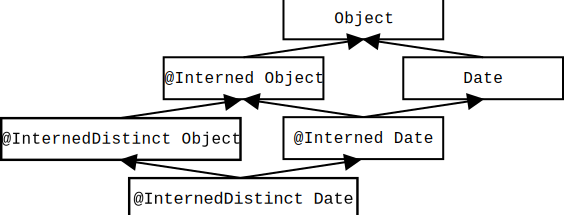
\includegraphics{figures/interning}}
\end{center}
%BEGIN LATEX
\vspace{-1.5\baselineskip}
%END LATEX
\caption{Type hierarchy for the Interning type system.}
\label{fig:interning-hierarchy}
\end{figure}

In order to perform checking, you must annotate your code with the \code{@\refclass{interning/quals}{Interned}}
type annotation, which indicates a type for the canonical representation of an
object:

\begin{Verbatim}
            String s1 = ...;  // type is (uninterned) "String"
  @Interned String s2 = ...;  // Java type is "String", but checker treats it as "Interned String"
\end{Verbatim}

The type system enforced by the checker plugin ensures that only interned
values can be assigned to \code{s2}.

To specify that \emph{all} objects of a given type are interned, annotate the
class declaration:

\begin{Verbatim}
  public @Interned class MyInternedClass { ... }
\end{Verbatim}

This is equivalent to annotating every use of \code{MyInternedClass}, in a
declaration or elsewhere.  For example, \code{enum} classes are implicitly
so annotated.


\subsection{Implicit qualifiers\label{interning-implicit-qualifiers}}

As described in Section~\ref{effective-qualifier}, the Interning checker
adds implicit qualifiers, reducing the number of annotations that must
appear in your code.
For example, String literals and the null literal are always considered interned, and
object creation expressions (using \code{new}) are never considered
\code{@\refclass{interning/quals}{Interned}} unless they are annotated as such, as in

%BEGIN LATEX
\begin{smaller}
%END LATEX
\begin{Verbatim}
@Interned Double internedDoubleZero = new @Interned Double(0); // canonical representation for Double zero
\end{Verbatim}
%BEGIN LATEX
\end{smaller}
%END LATEX

For a complete description of all implicit interning qualifiers, see the
Javadoc for \refclass{interning}{InterningAnnotatedTypeFactory}.


\section{What the Interning checker checks\label{interning-checks}}

Objects of an \code{@\refclass{interning/quals}{Interned}} type may be safely compared using the ``\code{==}''
operator.

The checker issues a warning in two cases:

\begin{enumerate}

\item
  When a reference (in)equality operator (``\code{==}'' or ``\code{!=}'')
  has an operand of non-\code{@\refclass{interning/quals}{Interned}} type.

\item
  When a non-\code{@\refclass{interning/quals}{Interned}} type is used where an \code{@\refclass{interning/quals}{Interned}} type
  is expected.

\end{enumerate}

This example shows both sorts of problems:

\begin{Verbatim}
            Object  obj;
  @Interned Object iobj;
  ...
  if (obj == iobj) { ... }  // checker warning: reference equality test is unsafe
  iobj = obj;               // checker warning: iobj's referent may no longer be interned
\end{Verbatim}

\label{lint-dotequals}

The checker also issues a warning when \code{.equals} is used where
\code{==} could be safely used.  You can disable this behavior via the
javac \code{-Alint} command-line option, like so: \code{-Alint=-dotequals}.

For a complete description of all checks performed by
  the checker, see the Javadoc for
  \refclass{interning}{InterningVisitor}.


\section{Examples\label{interning-example}}

To try the Interning checker on a source file that uses the \code{@\refclass{interning/quals}{Interned}} qualifier,
use the following command (where \code{javac} is the JSR 308 compiler that
is distributed with the Checker Framework):

\begin{Verbatim}
  javac -processor checkers.interning.InterningChecker examples/InterningExample.java
\end{Verbatim}

\noindent
Compilation will complete without warnings.

To see the checker warn about incorrect usage of annotations, use the following
command:

\begin{Verbatim}
  javac -processor checkers.interning.InterningChecker examples/InterningExampleWithWarnings.java
\end{Verbatim}

\noindent
The compiler will issue a warning regarding violation of the semantics of
\code{@\refclass{interning/quals}{Interned}}.
% in the \code{InterningExampleWithWarnings.java} file.


The Daikon invariant detector
(\myurl{http://groups.csail.mit.edu/pag/daikon/}) is also annotated with
\code{@\refclass{interning/quals}{Interned}}.  From directory \code{java},
run \code{make check-interning}.



% LocalWords:  plugin MyInternedClass enum InterningExampleWithWarnings java
% LocalWords:  PolyInterned Alint dotequals quals InterningAnnotatedTypeFactory
% LocalWords:  javac InterningVisitor

\htmlhr
\section{Lock checker\label{lock-checker}}

The Lock checker prevents certain kinds of concurrency errors.  If the Lock
checker issues no warnings for a given program, then the program holds the
appropriate lock every time that it accesses a variable.

Note:  This does \emph{not} mean that your program has no concurrency
errors.  (You might have forgotten to annotate that a particular variable
should only be accessed when a lock is held.  You might released and
re-acquire the lock, when correctness requires you to hold it throughout a
computation.  And, there are other concurrency errors that cannot, or
should not, be solved with locks.)  However, ensuring that your program
program obeys its locking discipline is an easy and effective way to
eliminate a common and important class of errors.


\subsection{Lock annotations\label{lock-annotations}}

The Lock checker uses two annotations.  One is a type qualifier, and the
other is a method annotation.

\begin{description}

\item[\code{@\refclass{lock/quals}{GuardedBy}}]
  indicates a type whose value may be accessed only when the given lock is
  held.  See the Javadoc for an explanation of the argument.  The lock
  acquisition and the field access may be arbitrarily far in the future.

\item[\code{@\refclass{lock/quals}{Holding}}]
  is a method annotation (not a type) qualifier.  It indicates that when
  the method is called, the given lock must be held by the caller.

\end{description}


A programmer may use the \code{@Holding} method annotation in two different ways.
\begin{itemize}
\item
  as specifying a higher-level synchronization protocol
\item
  as being a method summary that simplifies reasoning
\end{itemize}
\noindent
Both of these are useful, and the Lock checker supports both.
The latter (``summary'') use doesn't necessarily introduce a new
correctness constraint ``must hold this lock when accessing''.  Rather,
it expresses a fact about execution --- when execution reaches this
point, the following locks are held --- that enables people and tools to
reason intra- rather than inter-procedurally.  The point at which the
lock must be held for correctness may come later in the body of the
method or in a method it calls.


\subsubsection{Relationship to annotations in \emph{Java Concurrency in Practice}\label{jcip-annotations}}

The book \ahref{http://jcip.net/}{\emph{Java Concurrency in Practice}}~\cite{Goetz2006} defines a
\ahref{http://jcip.net/annotations/doc/net/jcip/annotations/GuardedBy.html}{\code{@GuardedBy}} annotation that is the inspiration for ours.  The book's
\code{@GuardedBy} serves two related purposes:

\begin{itemize}
\item
  When applied to a field, it means that the given lock must be held when
  accessing the field.  The lock acquisition and the field access may be
  arbitrarily far in the future.
\item
  When applied to a method, it means that the given lock must be held by
  the caller at the time that the method is called --- in other words, at
  the time that execution passes the \code{@GuardedBy} annotation.
\end{itemize}

One rationale for reusing the annotation name for both purposes in JCIP is
simplicity:  there are fewer annotations to learn.  Another rationale is
that both variables and methods are ``members'' that can be ``accessed'';
variables can be accessed by reading or writing them (putfield, getfield),
and methods can be accessed by calling them (invokevirtual,
invokeinterface).  In both cases,
\code{@GuardedBy} creates preconditions for accessing so-annotated members.

The Lock checker renames the method annotation to
\code{@\refclass{lock/quals}{Holding}}, and it generalizes the 
\code{@\refclass{lock/quals}{GuardedBy}} annotation into a type qualifier
that can apply not just to a field but to an arbitrary type (including the
type of a parameter, return value, local variable, generic type parameter,
etc.).  This makes the annotations more expressive and also more amenable
to automated checking.  It also accommodates the distinct (though related)
meaning of the two annotations.

% It would not work to retain the name \code{@GuardedBy} but put it on the
% receiver; an annotation on the receiver indicates what lock must be held
% when it is accessed in the future, not what must have already been held
% when the method was called.



% LocalWords:  quals GuardedBy JCIP putfield getfield invokevirtual
% LocalWords:  invokeinterface

%\htmlhr
\chapter{Index Checker for array bounds\label{index-checker}}

The Index Checker warns about unsafe array accesses.  It protects
against Java's
\sunjavadoc{java/lang/ArrayIndexOutOfBoundsException.html}{ArrayIndexOutOfBoundsException}. A
class checked by the
Index Checker  will not throw an ArrayIndexOutOfBoundException unless the
index has overflowed or underflowed. The Index Checker maintains information
for each sequence-like data structure and will report unsafe accesses to each.
It is designed primarily for arrays and Lists.

The Index Checker maintains an estimate of the range of values for each
index expression.  There are two ways an expression can fail to be safe for use as an
index: either it can be too low or it can be too high. The Index
Checker will warn about both types of dangerous accesses, and will
issue different warnings for the two.

Typically, programmers need to write only a few annotations to use the
Index Checker. The Index Checker will infer properties of indexes from
the code around them. For example, it will infer that \<x> is positive
within the then block of an \code{if (x > 0)} statement. However, the
Index Checker does not infer method pre-conditions or post-conditions,
which the programmer needs to write as annotations. For instance,
if an integer that is passed into a method is guaranteed to be a safe
index for the array ''myArray'', the programmer might need to
write an @IndexFor(''myArray'') annotation.


\section{Running the Index Checker\label{index-running}}

To run the Index Checker, run the command

\begin{alltt}
  javac -processor index \emph{MyJavaFile}.java
\end{alltt}

The Index Checker is a composition of several other checkers: the Lower
Bound Checker (section~\ref{index-lowerbound}), which checks whether potential accesses may be too low;
the Upper Bound Checker (section~\ref{index-upperbound}), which checks whether potential accesses
may be too high; the MinLen Checker (section~\ref{index-minlen}), which estimates the minimum
length of each sequence; and the SameLen Checker (section~\ref{index-samelen}), which finds arrays of equal length. All of the qualifiers of these subcheckers are considered ''index'' annotation (and warnings from any of them can be suppressed with @SuppressWarnings(''index''). In addition, the Index Checker maintains some qualifiers of its own, each of which is the combination of at least two qualifiers from different index subcheckers.

The Index annotations are:
\begin{description}
\item[\refqualclasswithparams{checker/index/qual}{IndexFor}{String[] names}]
  The value is a valid index for the named arrays. This type is the combination
  of the Lower Bound Checker's
  \refqualclass{checker/lowerbound/qual}{NonNegative} and the Upper Bound
  Checker's \refqualclasswithparams{checker/upperbound/qual}{LTLengthOf}{String[] names}.
 \item[\refqualclasswithparams{checker/index/qual}{IndexOrHigh}{String[] names}]
   The value is either a valid index for each named array, or equal to the
   length of one or more of the named arrays, and a valid index for the
   others. This type is the combination of the Lower Bound Checker's
  \refqualclass{checker/lowerbound/qual}{NonNegative} and the Upper Bound
  Checker's
  \refqualclasswithparams{checker/upperbound/qual}{LTEqLengthOf}{String[] names}.
\end{description}

\section{The Lower Bound Checker\label{index-lowerbound}}

The Lower Bound Checker warns about indices that might be
too low to access a zero-indexed sequence. The
Lower Bound Checker's type system uses the following qualifiers.

\begin{description}
\item[\refqualclass{checker/lowerbound/qual}{Positive}]
  The value is 1 or greater, so it is not too low to be used as an index.
\item[\refqualclass{checker/lowerbound/qual}{NonNegative}]
  The value is 0 or greater, so it is not too low to be used as an index.
\item[\refqualclass{checker/lowerbound/qual}{GTENegativeOne}]
  The value is -1 or greater.
  It may not be used as an index for a sequence, because it might be too low.
\item[\refqualclass{checker/lowerbound/qual}{LowerBoundUnknown}]
  There is no information about the value.
  It may not be used as an index for a sequence, because it might be too low.
\end{description}

\begin{figure}
  \includeimage{lowerbound}{7cm}
  \caption{The type hierarchy used by the Lower Bound Checker.}
  \label{fig-lowerbound-types}
\end{figure}

Typically, a programmer only needs to write these annotations on
fields and method signatures, because the Lower Bound Checker infers
qualifiers within method bodies.
In general, the Lower Bound Checker attempts to infer as much information
as possible from the source code.
Detailed documentation about the inferences performed can be found
in the Javadoc comments in its source code.


\section{The Upper Bound Checker\label{index-upperbound}}

The Upper Bound Checker warns about accesses to sequences with indexes that might be
too high.
The Upper Bound Checker's type system uses the following qualifiers.

\begin{description}
\item[\refqualclasswithparams{checker/upperbound/qual}{LTLengthOf}{String[] names}]
  An expression with this type
  has value less than the length of each sequence listed in \<names>.
  The expression may be used as an index into any of those sequences.
  \code{@LTLengthOf({"a", "b"})} is a subtype of both
  \code{@LTLengthOf("a")} and \code{@LTLengthOf("b")}.
\item[\refqualclasswithparams{checker/upperbound/qual}{LTEqLengthOf}{String[] names}]
  An expression with this type
  has value less than or equal to the length of each sequence listed in \<names>.
  It may not be used as an index for a sequence, because it might be too high.
  \code{@LTEqLengthOf({"a", "b"})} is a subtype of both
  \code{@LTEqLengthOf("a")} and \code{@LTEqLengthOf("b")}.
\item[\refqualclasswithparams{checker/upperbound/qual}{LTOMLengthOf}{String[] names}]
  An expression with this type
  has value less than one less than the length of each sequence listed in \<names>. This type exists to allow the checker to infer the safety of loops of
  the form:
\begin{Verbatim}
  for (int i = 0; i < array.length - 1; ++i) {
    arr[i] = arr[i+1];
  }
\end{Verbatim}
It may always used as an index for a sequence listed in \<names>, but
should rarely (if ever) be written by the programmer; usually
\refqualclasswithparams{checker/upperbound/qual}{LTLengthOf}{String[] names}
should be written instead.
  \code{@LTOMLengthOf({"a", "b"})} is a subtype of both
  \code{@LTOMLengthOf("a")} and \code{@LTOMLengthOf("b")}.
\item[\refqualclass{checker/upperbound/qual}{UpperBoundUnknown}]
  There is no information about the value of an expression with this type.
  It may not be used as an index for a sequence, because it might be too high.
  This type is the top type, and should never need to be written by the
  programmer.
\item[\refqualclass{checker/upperbound/qual}{UpperBoundBottom}]
  This is the bottom type for the Upper Bound type system. It should
  never need to be written by the programmer.
  \end{description}

\begin{figure}
  \includeimage{upperbound}{7cm}
  \caption{The type hierarchy used by the Upper Bound Checker.}
  \label{fig-upperbound-types}
\end{figure}

% Like the Lower Bound checker, the Upper Bound checker relies on both the Constant
% Value Checker and the MinLen checker. It uses the Constant Value Checker to determine
% precisely the value of particular indexes, and uses the MinLen checker both in the way
% described above (for constant indexes) and to determine when potential indexes should
% be assigned
% \refqualclasswithparams{checker/upperbound/qual}{LTLengthOf}{String[] names}] or
% \refqualclasswithparams{checker/upperbound/qual}{LTEqLengthOf}{String[] names}].

Typically, a programmer only needs to write these annotations on
fields and method signatures, because the Upper Bound Checker infers
qualifiers within method bodies.

\section{The MinLen Checker\label{index-minlen}}

The MinLen Checker estimates, for each sequence expression, how long its value
might be at run time.  The MinLen Checker computes a minimum length that
the sequence is guaranteed to have.

The main reason for the MinLen Checker is to handle fixed-length arrays
that are indexed by a compile-time constant.
There are two different situations when \<arr[i]> is legal because \<i> is
not too large:
\begin{itemize}
\item
  when \<i> is known to be less than the length of \<arr> independent of the length of
  \<arr>.  This fact is represented by giving \<i> the type \refqualclasswithparams{checker/upperbound/qual}{LTLengthOf}{"arr"}.
\item
  when \<i> is a compile-time constant but the length of \<arr> is known to
  be greater.  For example, consider the following code:
\end{itemize}

\begin{Verbatim}
  String getSecondElement(String[] arr) {
    return arr[1];
  }
\end{Verbatim}
  This is legal if \<arr> has at least two elements, which can be indicated
  in this way:
\begin{Verbatim}
  String getSecondElement(String @MinLen(2) [] arr) {
    return arr[1];
  }
\end{Verbatim}

The MinLen Checker uses the following type hierarchy:

\begin{description}
\item[\refqualclasswithparams{checker/minlen/qual}{MinLen}{int value}]
  An expression with this type represents a sequential structure
  with at least \code{value} elements.  The default annotation is
  \code{@MinLen(0)}, since an arbitrary object has at least 0 elements.
  In general, \code{@MinLen(x)} is a subtype of \code{@MinLen(x-1)}.
\item[\refqualclass{checker/minlen/qual}{MinLenBottom}]
  This is the bottom type for the MinLen type system.
  Programmers should rarely need to write it.
  \code{null} has this type.
  \end{description}

\begin{figure}
  \includeimage{minlen}{7cm}
  \caption{The type hierarchy used by the MinLen Checker.}
  \label{fig-minlen-types}
\end{figure}

\section{The SameLen Checker\label{index-samelen}}

The SameLen Checker determines whether sequences have the same length.

The main reason for the SameLen Checker is to handle cases where two
arrays are known to be the same length, and one is accessed using a
valid index for the other.

The SameLen Checker uses the following type hierarchy:

\begin{description}
  \item[\refqualclass{checker/samelen/qual}{SameLenUnknown}]
  This is the top type for the SameLen type system.
  Programmers should never need to write it, since it
  is automatically inferred for any expression that does
  not have a more specific type.
\item[\refqualclasswithparams{checker/samelen/qual}{SameLen}{String[] names}]
  An expression with this type represents a sequence that has the
  same length as the other sequences named in \<names>. In general,
  \code{@SameLen} types that have non-intersecting lists of names
  are \textit{not} subtypes of each other. However, if at least one
  sequence is named by both types, the types are actually the same,
  because all the named sequences must have the same length.
\item[\refqualclass{checker/samelen/qual}{SameLenBottom}]
  This is the bottom type for the SameLen type system.
  Programmers should rarely need to write it.
  \code{null} has this type.
  \end{description}

\begin{figure}
  \includeimage{samelen}{7cm}
  \caption{The type hierarchy used by the SameLen Checker.}
  \label{fig-samelen-types}
\end{figure}

\htmlhr
\chapterAndLabel{Called Methods Checker}{called-methods-checker}

The Called Methods Checker tracks the names of methods that have definitely been called
on each object in a program. This checker is useful for checking any property of the form
"call method A before method B." The Called Methods Checker provides built-in support for one
such property: that clients of classes that use the builder pattern for object construction
always provide all required arguments before calling \<build()>.

The builder pattern is a flexible and readable way to construct objects, but it is error-prone.
For example, failing to provide a required argument causes a run-time error that manifests during testing
or in the field, instead of at compile time as for regular Java constructors.

The Called Methods Checker verifies at compile time that your code correctly uses the builder pattern,
never omitting a required argument. The checker has built-in support for \href{https://projectlombok.org/}{Lombok}
(see the caveats about Lombok in \chapterpageref{called-methods-lombok}) and
\href{https://github.com/google/auto/blob/master/value/userguide/index.md}{AutoValue}.
Programmers can extend it to other builders by writing method specifications.

The Called Methods Checker can also be used to verify other properties of the form "foo() must be called
before bar()" if the user writes a custom specification; builders are a common example.
\chapterpageref{called-methods-other} describes another example related to a security property.

The checker performs verification rather than bug-finding.  The checker
might yield a false positive warning when your code is too tricky for it to
verify (please submit an
\href{https://github.com/typetools/checker-framework/issues}{issue} and mention the Called Methods Checker if
you discover this).  However, if the checker issues no warnings, then you
have a guarantee that your code supplies all the required information to
the builder.

\sectionAndLabel{How to run the Called Methods Checker}{called-methods-run-checker}

\begin{Verbatim}
javac -processor CalledMethods MyFile.java ...
\end{Verbatim}

\sectionAndLabel{For Lombok users}{called-methods-lombok}

The Called Methods Checker supports projects that use Lombok via
the \href{https://plugins.gradle.org/plugin/io.freefair.lombok}{io.freefair.lombok} Gradle plugin automatically.
However, note that the checker's error messages refer to Lombok's output, which is a variant of your source code
that appears in a \<delombok> directory.
To fix issues, you should edit your original source code, \textbf{not} the files in the checker's error messages.

If you use Lombok with a build system other than Gradle, you must configure it to do two tasks.
If either of these are not done, the checker will not issue any errors on Lombok code.
\begin{itemize}
\item set Lombok configuration option \<lombok.addLombokGeneratedAnnotation = true>
\item delombok the code before passing it to the checker
\end{itemize}

\sectionAndLabel{Specifying your code}{called-methods-spec}

The Called Methods Checker reads method specifications or contracts:  what a method requires when it is called.
It warns if method arguments do not satisfy the method's specification.

If you use AutoValue or Lombok, most specifications are automatically
inferred by the Called Methods Checker, from field annotations such as
\<@Nullable> and field types such as \<Optional>. See the
section on defaulting rules for Lombok and AutoValue for more details
(\chapterpageref{called-methods-framework-details}).

In some cases, you may need to specify your code. You do so by writing one of the following type
annotations:
\begin{description}
\item[\refqualclasswithparams{checker/CalledMethods/qual}{CalledMethods}{String[] methodNames}]
  The annotated type represents values on which all the given method were definitely called.
  (Other methods might also have been called.) \<@CalledMethods()> is the default annotation.

  Suppose that the method \<build> is annotated as

  \begin{Verbatim}
  class MyObjectBuilder {
    MyObject build(@CalledMethods({"setX", "setY"}) MyObjectBuilder this) { ... }
  }
  \end{Verbatim}

  Then the receiver for any call to \<build()> must have had \<setX()> and \<setY()> called on it.

\item[\refqualclasswithparams{checker/CalledMethods/qual}{CalledMethodsPredicate}{String expression}]
  The annotated type specifies the required method calls using a Java boolean syntax that supports
  disjunction (\<||>), conjunction (\<\&\&>), parentheses, and not (\<!>).

  For example, the annotation \<@CalledMethodsPredicate("x \&\& y || z")> on a type represents
  objects such that either both the  \<x()> and \<y()> methods have been called on the object, \textbf{or}
  the \<z()> method has been called on the object.

  A note on the not operator (\<!?>): the annotation \<@CalledMethodsPredicate("!x")> means: "it is not true x was
  definitely called", equivalently "there is some path on which x was not called".
  The annotation \<@CalledMethodsPredicate("!x")> does \emph{not} mean "x was not called".

  The Called Methods Checker does not have a way of expressing that a
  method must never be called.  You can do unsound bug-finding for such a
  property by using the `!` operator.  The Called Methods Checker will
  detect if the method was always called, but will silently approve the code
  if the method is called on some but not all paths.

\item[\refqualclass{checker/CalledMethods/qual}{EnsuresCalledMethods}]
  This declaration annotation specifies a post-condition on a method, indicating the methods it
  guarantees to be called on some input expression.

  For example, this specification:

  \begin{Verbatim}
    @EnsuresCalledMethods(value = "#1", methods = {"x","y"})
    void m(Param p) { ... }
  \end{Verbatim}

  guarantees that \<p.x()> and \<p.y()> will always be called before \<m> returns.
  The body of \<m> must satisfy that property, and clients of \<m> can depend on the property.

\item[\refqualclass{common/returnsreceiver/qual}{This}]
  \<@This> may only be written on a method return type, and means that the method returns its receiver.
  This is helpful when type-checking fluent APIs. This annotation is defined by the
  Returns Receiver Checker (\chapterpageref{returns-receiver-checker}), but is particularly useful
  for the Called Methods Checker because many builders are fluent APIs.

\end{description}

\sectionAndLabel{Default handling for Lombok and AutoValue}{called-methods-framework-details}

This section gives detailed rules on how the Called Methods Checker infers types for the Lombok
and AutoValue frameworks. Most readers can skip these details.

The Called Methods Checker automatically assumes default annotations for code that uses builders generated
by Lombok and AutoValue. There are three places annotations are usually assumed:
\begin{itemize}
\item An \<@CalledMethods> annotation is placed on the receiver of the \<build()> method, capturing the
setter methods that must be invoked on the builder before calling \<build()>. For Lombok,
this annotation's argument is the set of \<@lombok.NonNull> fields that do not have default values.
For AutoValue, it is the set of fields that are not \<@Nullable>, \<Optional>, or a Guava Immutable
Collection.
\item If the object has a \<toBuilder()> method (for example, if the \<toBuilder = true> option is
passed to Lombok's \<@Builder> annotation), then the return type of that method is annotated with
the same \<@CalledMethods> annotation as the receiver of \<build()>, using the same rules as above.
\item An \<@This> annotation is placed on the return type of each setter in the builder's implementation.
\end{itemize}

You can disable the framework supports by specifying them in a comma-separated list to the
command-line flag \<disableFrameworkSupports>.  For example, to disable both Lombok and AutoValue supports,
use \<-ACalledMethodsChecker_disableFrameworkSupports=AutoValue,Lombok>.

If you overwrite the definition of any of these methods (for example, by adding your own setters to
a Lombok builder), you may need to write the annotations manually.

Minor notes/caveats on these rules:
\begin{itemize}
\item Lombok fields annotated with \<@Singular> will be treated as defaulted (i.e. not required), because
Lombok will set them to empty collections if the appropriate setter is not called.
\item If you manually provide defaults to a Lombok builder (for example, by defining the builder yourself
and assigning a default value to the builder's field), the checker will treat that field as defaulted
\emph{most} of the time. In particular, it will not treat it as defaulted if it is defined in bytecode rather
than in source code.
\end{itemize}

\sectionAndLabel{Using the Called Methods Checker for properties unrelated to builders}{called-methods-other}

The Called Methods Checker can be used to verify any property of the form "always call A before B", even
if the property is unrelated to builders. For example, consider the AWS EC2 \<describeImages> API, which
clients use during the process of initializing a new cloud instance.
\href{https://cve.mitre.org/cgi-bin/cvename.cgi?name=CVE-2018-15869}{CVE-2018-15869} describes how an
improperly-configured request to this API can make the requesting client vulnerable to a "machine-image sniping"
attack that would allow a malicious third-party to control the operating system image used to initialize the
machine. To prevent this attack, clients must specify some trusted source for the image by calling the
\<withOwners> or \<withImageIds> methods on the request prior to sending it to AWS. Using a stub file for the
\<describeImages> API
(\href{https://github.com/typetools/checker-framework/blob/master/checker/src/main/java/org/checkerframework/calledmethods/DescribeImages.astub}{DescribeImages.astub}),
the Called Methods Checker can prove that a client is not vulnerable to such an attack. To improve precision,
the \<-ACalledMethodsChecker\_useValueChecker> command-line option to treat provably-safe calls to the \<withFilters>
method of a \<DescribeImagesRequest> as equivalent to the \<withOwners> or \<withImageIds> methods.

\htmlhr
\chapter{Fake Enum Checker for fake enumerations\label{fenum-checker}}

The Fake Enum Checker, or Fenum Checker, enables you to define a type alias
or typedef, in which two different sets of values have the same
representation (the same Java type) but are not allowed to be used
interchangeably.  It is also possible to create a typedef using the
Subtyping Checker (\chapterpageref{subtyping-checker}), and that approach
is sometimes more appropriate.

One common use for the Fake Enum Checker is the
\emph{fake enumeration pattern} (Section~\ref{fenum-pattern}).  For
example, consider this code adapted from Android's
\href{https://developer.android.com/reference/android/support/annotation/IntDef.html}{\code{IntDef}}
documentation:

\begin{Verbatim}
@NavigationMode int NAVIGATION_MODE_STANDARD = 0;
@NavigationMode int NAVIGATION_MODE_LIST = 1;
@NavigationMode int NAVIGATION_MODE_TABS = 2;

@NavigationMode int getNavigationMode();

void setNavigationMode(@NavigationMode int mode);
\end{Verbatim}

The Fake Enum Checker can issue a compile-time warning if the programmer
ever tries to call \<setNavigationMode> with an \<int> that is not a
\<@NavigationMode int>.

The Fake Enum Checker gives the same safety guarantees as a true enumeration
type or typedef, but retaining backward-compatibility with interfaces that
use existing Java types.  You can apply fenum annotations to any Java type,
including all primitive types and also reference types.  Thus, you could
use it (for example) to represent floating-point values between 0 and 1, or
\<String>s with some particular characteristic.
(Note that the Fake Enum Checker does not let you create a shorter alias
for a long type name, as a real typedef would if Java supported it.)

As explained in Section~\ref{fenum-annotations}, you can either define your
own fenum annotations, such as \<@NavigationMode> above, or you can use the
existing \refqualclass{checker/fenum/qual}{Fenum} with a string argument.
Figure~\ref{fig-fenum-hierarchy} shows part of the type hierarchy for the
Fenum type system.

\begin{figure}
\includeimage{fenum}{3.2cm}
\caption{Partial type hierarchy for the Fenum type system.
There are two forms of fake enumeration annotations --- above, illustrated
by \code{@Fenum("A")} and \code{@FenumC}.
See Section~\ref{fenum-annotations} for descriptions of how to
introduce both types of fenums. The type qualifiers in gray
(\code{@FenumTop}, \code{@FenumUnqualified}, and \code{@FenumBottom})
should never be written in
source code; they are used internally by the type system.
\<@FenumUnqualified> is the default qualifier for unannotated types, except
for upper bounds which default to \<@FenumTop>.
}
\label{fig-fenum-hierarchy}
\end{figure}

\section{Fake enum annotations\label{fenum-annotations}}

The Fake Enum Checker supports two ways to introduce a new fake enum (fenum):

\begin{enumerate}
\item Introduce your own specialized fenum annotation with code like this in
file \code{\emph{MyFenum}.java}:

\begin{alltt}
package \textit{myPackage}.qual;

import java.lang.annotation.Documented;
import java.lang.annotation.ElementType;
import java.lang.annotation.Retention;
import java.lang.annotation.RetentionPolicy;
import java.lang.annotation.Target;
import org.checkerframework.checker.fenum.qual.FenumTop;
import org.checkerframework.framework.qual.SubtypeOf;

@Documented
@Retention(RetentionPolicy.RUNTIME)
@Target(\ttlcb{}ElementType.TYPE_USE, ElementType.TYPE_PARAMETER\ttrcb)
@SubtypeOf(FenumTop.class)
public @interface \textit{MyFenum} \ttlcb\ttrcb
\end{alltt}

You only need to adapt the italicized package, annotation, and file names in the example.

Note that all custom annotations must have the
\<@Target(\ttlcb ElementType.TYPE\_USE\ttrcb)> meta-annotation. See section
\ref{creating-define-type-qualifiers}.

\item Use the provided \refqualclass{checker/fenum/qual}{Fenum} annotation, which takes a
\code{String} argument to distinguish different fenums or type aliases.
For example, \code{@Fenum("A")} and \code{@Fenum("B")} are two distinct
type qualifiers.
\end{enumerate}


The first approach allows you to define a short, meaningful name suitable for
your project, whereas the second approach allows quick prototyping.



\section{What the Fenum Checker checks\label{fenum-checks}}

The Fenum Checker ensures that unrelated types are not mixed.
All types with a particular fenum annotation, or \code{@Fenum(...)} with a
particular \code{String} argument, are
disjoint from all unannotated types and from all types with a different fenum
annotation or \code{String} argument.

The checker ensures that
only compatible fenum types are used in comparisons and arithmetic operations
(if applicable to the annotated type).

It is the programmer's responsibility to ensure that fields with a fenum type
are properly initialized before use.  Otherwise, one might observe a \code{null}
reference or zero value in the field of a fenum type.  (The Nullness Checker
(\chapterpageref{nullness-checker}) can prevent failure to initialize a
reference variable.)


\section{Running the Fenum Checker\label{fenum-running}}

The Fenum Checker can be invoked by running the following commands.

\begin{itemize}
  \item
If you define your own annotation(s), provide the name(s) of the annotation(s)
through the \code{-Aquals} option, using a comma-no-space-separated notation:

\begin{alltt}
  javac -classpath \textit{/full/path/to/myProject/bin}:\textit{/full/path/to/myLibrary/bin} \ttbs
        -processor org.checkerframework.checker.fenum.FenumChecker \ttbs
        -Aquals=\textit{myPackage.qual.MyFenum} MyFile.java ...
\end{alltt}

The annotations listed in \code{-Aquals} must be accessible to
the compiler during compilation in the classpath.  In other words, they must
already be compiled (and, typically, be on the javac classpath)
before you run the Fenum Checker with \code{javac}.  It
is not sufficient to supply their source files on the command line.

You can also provide the fully-qualified paths to a set of directories
that contain the annotations through the \code{-AqualDirs} option,
using a colon-no-space-separated notation. For example:

\begin{alltt}
  javac -classpath \textit{/full/path/to/myProject/bin}:\textit{/full/path/to/myLibrary/bin} \ttbs
        -processor org.checkerframework.checker.fenum.FenumChecker \ttbs
        -AqualDirs=\textit{/full/path/to/myProject/bin}:\textit{/full/path/to/myLibrary/bin} MyFile.java ...
\end{alltt}

Note that in these two examples, the compiled class file of the
\<myPackage.qual.MyFenum> annotation must exist in either the \<myProject/bin>
directory or the \<myLibrary/bin> directory. The following placement of
the class file will work with the above commands:

\begin{alltt}
  .../myProject/bin/myPackage/qual/MyFenum.class
\end{alltt}

The two options can be used at the same time to provide groups of annotations
from directories, and individually named annotations.

\item
If your code uses the \refqualclass{checker/fenum/qual}{Fenum} annotation, you do
not need the \code{-Aquals} or \code{-AqualDirs} option:

\begin{Verbatim}
  javac -processor org.checkerframework.checker.fenum.FenumChecker MyFile.java ...
\end{Verbatim}

\end{itemize}

For an example of running the Fake Enum Checker on Android code, see
\url{https://github.com/karlicoss/checker-fenum-android-demo}.


\section{Suppressing warnings\label{fenum-suppressing}}

One example of when you need to suppress warnings is when you initialize the
fenum constants to literal values.
To remove this warning message, add a \code{@SuppressWarnings} annotation to either
the field or class declaration, for example:

\begin{Verbatim}
@SuppressWarnings("fenum:assignment.type.incompatible") // initialization of fake enums
class MyConsts {
  public static final @Fenum("A") int ACONST1 = 1;
  public static final @Fenum("A") int ACONST2 = 2;
}
\end{Verbatim}



\section{Example\label{fenum-example}}

The following example introduces two fenums in class \code{TestStatic}
and then performs a few typical operations.

\begin{Verbatim}
@SuppressWarnings("fenum:assignment.type.incompatible")   // initialization of fake enums
public class TestStatic {
  public static final @Fenum("A") int ACONST1 = 1;
  public static final @Fenum("A") int ACONST2 = 2;

  public static final @Fenum("B") int BCONST1 = 4;
  public static final @Fenum("B") int BCONST2 = 5;
}

class FenumUser {
  @Fenum("A") int state1 = TestStatic.ACONST1;     // ok
  @Fenum("B") int state2 = TestStatic.ACONST1;     // Incompatible fenums forbidden!

  void fenumArg(@Fenum("A") int p) {}

  void foo() {
    state1 = 4;                     // Direct use of value forbidden!
    state1 = TestStatic.BCONST1;    // Incompatible fenums forbidden!
    state1 = TestStatic.ACONST2;    // ok

    fenumArg(5);                    // Direct use of value forbidden!
    fenumArg(TestStatic.BCONST1);   // Incompatible fenums forbidden!
    fenumArg(TestStatic.ACONST1);   // ok
  }
 }
\end{Verbatim}

Also, see the example project in the \<docs/examples/fenum-extension> directory.


\section{The fake enumeration pattern\label{fenum-pattern}}

Java's
\href{https://docs.oracle.com/javase/specs/jls/se8/html/jls-8.html#jls-8.9}{\code{enum}}
keyword lets you define an enumeration type: a finite set of distinct values
that are related to one another but are disjoint from all other
types, including other enumerations.
Before enums were added to Java, there were two ways to encode an
enumeration, both of which are error-prone:

\begin{description}
\item[the fake enum pattern]  a set of \code{int} or \code{String}
  constants (as often found in older C code).

\item[the \href{http://www.oracle.com/technetwork/java/page1-139488.html}{typesafe
enum pattern}]  a class with private constructor.
% This requires
% \href{http://www.javaworld.com/javaworld/javatips/jw-javatip122.html}{careful development}.
\end{description}

Sometimes you need to use the fake enum pattern,
rather than a real enum or the typesafe enum pattern.
%
One reason is backward-compatibility.  A public API that predates Java's
enum keyword may use \code{int} constants; it cannot be changed, because
doing so would break existing clients.  For example, Java's JDK still uses
\code{int} constants in the AWT and Swing frameworks, and Android also uses
\code{int} constants rather than Java enums.
%
Another reason is performance, especially in environments with limited
resources.  Use of an int instead of an object can
reduce code size, memory requirements, and run time.
% Android no longer recommends use of ints instead of enums:  see
% http://stackoverflow.com/questions/5143256/why-was-avoid-enums-where-you-only-need-ints-removed-from-androids-performanc

In cases when code has to use the fake enum pattern, the Fake Enum Checker,
or Fenum Checker, gives the same safety guarantees as a true enumeration type.
The developer can introduce new types that are distinct from all values of the
base type and from all other fake enums. Fenums can be introduced for
primitive types as well as for reference types.


\section{References\label{fenum-references}}

\begin{itemize}
\item Case studies of the Fake Enum Checker:\\
  ``Building and using pluggable type-checkers''~\cite{DietlDEMS2011}
  (ICSE 2011, \url{http://homes.cs.washington.edu/~mernst/pubs/pluggable-checkers-icse2011.pdf#page=3})

\item Java Language Specification on enums:\\
  \url{https://docs.oracle.com/javase/specs/jls/se8/html/jls-8.html#jls-8.9}

\item Tutorial trail on enums:\\
  \url{https://docs.oracle.com/javase/tutorial/java/javaOO/enum.html}

\item Typesafe enum pattern:\\
  \url{http://www.oracle.com/technetwork/java/page1-139488.html}

\item Java Tip 122: Beware of Java typesafe enumerations:\\
  \url{http://www.javaworld.com/article/2077487/core-java/java-tip-122--beware-of-java-typesafe-enumerations.html}

\end{itemize}

% LocalWords:  enums typesafe Fenum Fenums fenum MyFenum quals fenums Aquals
% LocalWords:  TestStatic FenumC FenumD myPackage RetentionPolicy IntDef
% LocalWords:  SubtypeOf FenumTop MyFile Enum enum AWT java jls qual
%  LocalWords:  FenumUnqualified FenumBottom ElementType classpath
%%  LocalWords:  bootclasspath AqualDirs myProject myLibrary
%  LocalWords:  setNavigationMode NavigationMode

\htmlhr
\chapter{Tainting checker\label{tainting-checker}}

The tainting checker prevents certain kinds of trust errors.
A \emph{tainted}, or untrusted, value is one that comes from an arbitrary,
possibly malicious source, such as user input or unvalidated data.
Using a tainted value in certain parts of your application can compromise
its integrity, causing it to crash, corrupt data, leak private data, etc.

% Ought to have many more examples

For example, a user-supplied pointer, handle, or map key should be
validated before being dereferenced.
As another example, user-supplied strings should not be concatenated into a
SQL query, program be subject to a 
\ahref{http://en.wikipedia.org/wiki/Sql_injection}{SQL injection} attack.
A location in your program where malicious data could do damage is
called a \emph{sensitive sink}.

A program can ``sanitize'' or ``untaint'' a value in two ways:  by checking
that it is innocuous/legal (e.g., it contains no characters that can be
interpreted as SQL commands when pasted into a string context), or by
transforming the value to be legal (e.g., quoting all the characters that
can be interpreted as SQL commands).  A correct program must use one of
these two techniques so that tainted values never flow to a sensitive sink.
The Tainting Checker ensures that your program does so.

If the Tainting Checker issues no warning for a given program, then no
tainted value ever flows to a sensitive sink.  However, your program is not
necessarily free from all trust errors.  As a simple example, you might
have forgotten to annotate a sensitive sink as requiring an untainted type.


\section{Tainting annotations\label{tainting-annotations}}

% TODO: add both qualifiers explicitly, and then describe their relationship.

The Tainting type system uses one annotation:
\code{@\refclass{tainting/quals}{Untainted}}.  The annotation indicates
a type that includes only untainted, trusted values.

Any type not marked as \code{Untainted} is treated as tainted, or untrusted.


\section{Writing \code{@Untainted} annotations\label{writing-untainted}}

In order to use the tainting checker, you must annotate your code with
\code{@\refclass{tainting/quals}{Untainted}} type annotation, to mark
operations that require trusted operations.

It is helpful to start annotating the secure kernel boundary entry
points.  To secure against SQL injection attacks, it is useful to
start annotating the \sunjavadoc{java/sql/Statement.html}{Statement}
class; the execute operations may only operate on untainted queries
(Chapter~\ref{annotating-libraries} describes how you can annotate
external libraries)

\begin{Verbatim}
  public boolean execute(@Untainted String sql) throws SQLException;
  public boolean executeUpdate(@Untainted String sql) throws SQLException; 
\end{Verbatim}

The Tainting checker, in turn, will verify that no untainted value may flow into
any of these methods.

% LocalWords:  quals untaint


% These are focused on strings:
\htmlhr
\chapter{Regex checker for regular expression syntax\label{regex-checker}}

The Regex Checker prevents, at compile-time, use of syntactically invalid
regular expressions.

A regular expression, or regex, is a pattern for matching certain strings
of text.  In Java, a programmer writes a regular expression as a string.
At run time, the string is ``compiled'' into an efficient internal form
(\sunjavadoc{java/util/regex/Pattern.html}{Pattern}) that is used for
text-matching.

The syntax of regular expressions is complex, so it is easy to make a
mistake.  It is also easy to accidentally use a regex feature from another
language that is not supported by Java (see section ``Comparison to Perl
5'' in the \sunjavadoc{java/util/regex/Pattern.html}{Pattern} Javadoc).
Ordinarily, the programmer does not learn of these errors until run time.
The Regex checker warns about these problems at compile time.

To run the Regex Checker, supply the \code{-processor
  checkers.regex.RegexChecker} command-line option to javac.


\section{Regex annotations\label{regex-annotations}}

The Regex Checker uses one annotation only:
\code{@\refclass{regex/quals}{Regex}}, to indicate valid regular
expression \code{String}s.

The checker implicitly adds the \code{Regex} qualifier to any
\code{String} literal that is a valid regex.


% LocalWords:  Regex regex quals

\htmlhr
\chapter{Format String Checker\label{formatter-checker}}

% VERIFICATION
The Format String Checker detects and prevents use of incorrect format strings
in format methods such as 
\sunjavadoc{java/io/PrintStream.html#printf(java.lang.String,java.lang.Object...)}{System.out.printf}
and \sunjavadoc{java/lang/String.html#format(java.lang.String, java.lang.Object...)}{String.format}.
% BUG FINDER
% The Format String Checker helps to prevent bugs that are the result of an
% incorrect use of format methods such as 
% \sunjavadoc{java/io/PrintStream.html#printf(java.lang.String,java.lang.Object...)}{System.out.printf}.

% VERIFICATION

% BUG FINDER
% The Format String Checker helps to prevent bugs in two ways: 
% 
% \begin{itemize}
% \item An error is issued if a format method would fail to execute at
%     runtime.  For example, if an invalid format string is passed.  
% \item A warning is issued for possibly legal but likely unintended uses of a
%     format method. For example, if unused format arguments are passed. 
% \end{itemize}
%
% \noindent
Following are examples of common errors that the Format String Checker detects at
compile time, more details are provided in Section~\ref{formatter-bugs}.

\begin{Verbatim}
    String.format("%d", "String");  // invalid argument for %d
    String.format("%y", 7);         // invalid format string
    String.format("{0}", "String"); // unused argument, {0} is wrong syntax
    String.format("%d", 7, 3);      // unused argument 3
    String.format("%d %s", 7);      // missing argument for %s
\end{Verbatim}

The Format String Checker's most important annotation is
\code{@\refclass{checker/quals}{Format}}. Yet, it is rare that this annotation
has to be written, as it is inferred if a string literal is directly passed as
a format method's first parameter. The Format String Checker's annotations are
explained in Section~\ref{formatter-annotations}.

To run the Format String Checker, supply the \code{-processor
checkers.formatter.FormatterChecker} command-line option to javac. 

\section{Format String Checker annotations\label{formatter-annotations}}

Printf-style formatting is the process of replacing \emph{format specifiers} in
a \emph{format string}. The replacements are taken from a \emph{format argument}
list, and the format specifier determines how the format argument is converted to a
string. The Java standard library provides printf-style formatting in \emph{format methods} such as
\sunjavadoc{java/lang/String.html#format(java.lang.String, java.lang.Object...)}{String.format}
and 
\sunjavadoc{java/io/PrintStream.html#printf(java.lang.String,java.lang.Object...)}{System.out.printf}.
Format specifiers are introduced by a \code{\%} character. For example,
\code{String.format("\%s \%d","str",1)} yields \code{"str 1"}.  \code{"\%s \%d"} is
the format string, \code{"\%s"} and \code{"\%d"} are the format specifiers;
\code{"str"} and \code{1} are format arguments.  All of Java's format
methods use the \sunjavadoc{java/util/Formatter.html}{Formatter} class internally.

The Formatter Checker assigns a qualifier to every term, in addition to the
regular Java type. These qualifiers make up the Format String type system.

The \code{@\refclass{formatter/quals}{Format}} qualifier indicates a
\emph{valid} format string. A format string \code{s} is valid if there exists a
list of format arguments \code{l}, such that \code{String.format(s,l)}
does not throw an exception. 

Passing a valid format string to a format method does not guarantee that the 
invocation will succeed. The format method invocation \code{String.format("\%d","String")}
for example, will fail despite the fact that \code{"\%d"} is valid. Passing
a valid format string to a format method with all format arguments being \code{null}, will
never throw an exception.

The \code{@\refclass{formatter/quals}{Format}} qualifier is parameterized with
a list of conversion categories that impose restricts on the format arguments.
Conversion categories are explained in more detail in
Section~\ref{formatter-categories}.  The type qualifier for \code{"\%d \%f"} is
for example \code{@Format(\{INT, FLOAT\})}.

The following example shows how to use the \code{@Format} annotation to
enforces that the function's parameter is a format string that, when
passed to a format method, requires the first format argument to be ``float like'',
and the second format argument to be ``integer like'':

\begin{Verbatim}
    void print(@Format({FLOAT, INT}) format) {
        System.out.printf(format, 7.8, 7);
    } 

    print("Float %f, Number %d");  // ok
    print("Float %f");             // error
\end{Verbatim}

\noindent All other annotations in the Format String type system are only used
internally and cannot be written in your code.
\code{@\refclass{formatter/quals}{InvalidFormat}} indicates an invalid format
string. The annotation is attached to \code{"\%y"}
for example.  \code{@\refclass{formatter/quals}{FormatBottom}} is assigned to the
\code{null} literal. All other terms are assigned the
\code{@\refclass{formatter/quals}{Unqualified}} qualifier.

\subsection{Conversion Categories\label{formatter-categories}}

A format specifier's conversion component consists of its last, or the last two,
characters. The conversion component of \code{"\%d"} is for example \code{d}.

The format argument used to replace a format specifier, may be restricted 
by the format specifier's conversion component. In the following example, the
format specifier's conversion component \code{d} restricts the first format argument
to be ``integer like'':

\begin{Verbatim}
    String.format("%d", 5);         // ok
    String.format("%d", "String");  // warning
\end{Verbatim}

\noindent Many conversion components enforce the same restrictions. We represent
these restrictions as a set of allowed values called \emph{conversion
category}. The ``integer like'' restriction is for example the conversion
category INT.  The following conversion categories are defined in the
\code{\refclass{formatter/quals}{ConversionCategory}} enumeration:

\begin{description}
\item{GENERAL} imposes no restrictions on a format argument's type. Applicable for
    conversions b, B, h, H, s, S.

\item{CHAR} requires that a format argument represents a Unicode character.
    Specifically, \code{char}, \code{Character}, \code{byte},
    \code{Byte}, \code{short}, and \code{Short} are allowed.
    \code{int} or \code{Integer} are allowed if
    \code{Character.isValidCodePoint(argument)} would return \code{true}
    for the format argument. Applicable for conversions c, C.

\item{INT} requires that a format argument represents an integral type. Specifically,
    \code{byte}, \code{Byte}, \code{short}, \code{Short},
    \code{int} and \code{Integer}, \code{long},
    \code{Long}, and \code{BigInteger} are allowed. Applicable for
    conversions d, o, x, X.  

\item{FLOAT} requires that a format argument represents a floating-point type.  Specifically,
    \code{float}, \code{Float}, \code{double},
    \code{Double}, and \code{BigDecimal} are allowed. Surprisingly, integer
    values are not allowed. Applicable for
    conversions e, E, f, g, G, a, A.
 
\item{TIME} requires that a format argument represents a date or time.
    Specifically, \code{long}, \code{Long}, \code{Calendar}, and
    \code{Date} are allowed.  Applicable for conversions t, T.

\item{UNUSED} imposes no restrictions on a format argument. This is the case if a
    format argument is not used as replacement for any format specifier.
    \code{"\%2\$s"} for example ignores the first format argument. 
    % This conversion category is similar to GENERAL, but does allow objects that
    % throw exceptions in \code{toString} and \code{formatTo}.
\end{description}

\noindent Further, all conversion categories accept \code{null}.
% MAKES SENSE, BUT IS CONFUSING AND NOT REALLY RELEVEVANT
% Unless otherwise noted, do not allow objects whose \code{toString} method throws an exception.
% Objects that implement the \code{Formattable} interface and throw an
% exception in \code{formatTo} are also not allowed.

Until now, we have assumed that the format specifiers simply consume format arguments left to right.
But there are two other ways for a format specifier to select a format argument:

\begin{itemize}
\item One can specify a one-based \emph{index} before a \code{\$} sign. In the
    format string \code{"\%2\$s"} for example, the format specifier selects the
    second format argument.  
\item One can pass the \code{<} \emph{flag} to reference the format argument
    that was used by the previous format specifier. In the format string
    \code{"\%d \%<d"} for example, both format specifiers select the first
    format argument.
\end{itemize}

\noindent The same format argument may serve as replacement for multiple format specifiers. In
this case, the format argument is restricted by multiple conversions, and is therefore the
\emph{intersection} of the associated conversion categories. 

In the following example, the format argument is restricted by CHAR and
INT.  The format argument must therefore be compatible with both conversion
categories, and can therefore neither be a \code{Character} nor \code{Long}.
This particular intersection of conversion categories is called
\code{CHAR\_AND\_INT}:

\begin{Verbatim}
    format("Char %1$c, Int %1$d", (int)42);   // ok
    format("Char %1$c, Int %1$d", (long)42);  // error
\end{Verbatim}
 
\noindent Many of these intersections lead to already existing conversion categories,
for example \code{GENERAL} $\cap$ \code{CHAR} $=$ \code{CHAR} and 
\code{UNUSED} $\cap$ \code{GENERAL} $=$ \code{GENERAL}. But some do not:

\begin{description}
\item{NULL} is used if no object of any type can be
    passed as parameter. In this case, the only legal value is \code{null}.
    The format string \code{"\%1\$f \%1\$c"}, for example requires that the first
    format argument be \code{null}.  Passing a value such as \code{4} or
    \code{4.2} would lead to an exception.
\item{CHAR\_AND\_INT} is used if a format argument is restricted by a \code{CHAR} and \code{INT} conversion category (\code{CHAR} $\cap$ \code{INT}).
\item{INT\_AND\_TIME} is used if a format argument is restricted by an \code{INT} and \code{TIME} conversion category (\code{INT} $\cap$ \code{TIME}).
\end{description}

\noindent All intersections of more than two conversion categories lead to an already
existing conversion category. Figure~\ref{fig:formatter-cat} summarizes the subset 
relationship among all conversion categories.

\begin{figure}[thbp]
    \includeimage{formatter-categories}{2.5cm}
    \caption{The subset relationship among conversion categories.}
    \label{fig:formatter-cat}
\end{figure}

\subsection{Type Hierarchy}

\begin{figure}[thbp]
\includeimage{formatter-hierarchy}{2.5cm}
\caption{The Format String Checker type hierarchy.}
\label{fig:formatter-th}
\end{figure}

\noindent Figure~\ref{fig:formatter-th} summarizes the subtype relation among all type
qualifiers.  

% THIS SHOULD BE IN A MORE GENERAL DESCRIPTION OF THE FRAMEWORK
% \code{@Unqualified} is at the top of the hierarchy, which reduces
% false positives. Among other things, it allows you to pass format strings into
% functions that require a simple String without any qualifiers. The \code{null}
% value is assigned bottom for similar reasons. In the following example, this
% enables us to know that no matter the qualifier of \code{T}, \code{null} can
% always be assigned to it:
% 
% \begin{Verbatim}
%     <T> T f() {
%         return null;
%     }
% \end{Verbatim}

Not shown in the figure are the subtyping rules among \code{@Format} qualifiers
with different conversion categories. It is legal to:

\begin{itemize}
\item use a format string with a weaker (less restrictive) conversion category than required.
\item use a format string with less format specifiers than required, but a warning is issued. 
\end{itemize}

The following example shows the subtyping rules in action:

\begin{Verbatim}
    @Format({FLOAT, INT}) 
    String f;

    f = "%f %d";       // ok
    f = "%s %d";       // ok, %s weaker than %f
    f = "%f";          // warning, last argument ignored
    f = "%f %d %s";    // error, too many arguments
    f = "%d %d";       // error, %d not weaker than %f

    String.format(f, 0.8, 42);
\end{Verbatim}

\section{What does the Format String Checker check\label{formatter-bugs}}

% VERIFICATION
If the Format String Checker issues no errors, it provides the following guarantees:

\noindent I.) The following guarantees hold for every format method invocation:

\begin{enumerate} 
    \item The format method's first parameter (or second if a \sunjavadoc{java/util/Locale}{Locale} is provided) is a valid 
        format string (or \code{null}).
    \item A warning is issued if one of the format string's conversion categories is \code{UNUSED}.
    \item None of the format string's conversion categories is \code{NULL}.
\end{enumerate} 

\noindent II.) If the format arguments are passed to the format method as varargs, the
Format String Checker guarantees the following additional properties:

\begin{enumerate} 
\item No fewer format arguments are passed than required by the format string.
\item A warning is issued, if more format arguments are passed than required by the format string.
\item Every format argument's type satisfies its conversion category's restrictions.
\end{enumerate}

\noindent III.) If the format arguments are passed to the format method as array, 
an warning is issued by the Format String Checker.

\noindent Following are examples for every guarantee:

\begin{Verbatim}
    String.format("%d", 42);                     // ok
    String.format(Locale.GERMAN, "%d", 42);      // ok
    String.format(new Object());                 // error (I 1)
    String.format("%y");                         // error (I 1)
    String.format("%2$s","unused","used");       // warning (I 2)
    String.format("%1$d %1$f", 5.5);             // error (I 3)
    String.format("%1$d %1$f %d", null, 6);      // error (I 3)
    String.format("%s");                         // error (II 1)
    String.format("%s","used","ignored");        // warning (II 2)
    String.format("%c",4.2);                     // error (II 3)
    String.format("%c",(String)null);            // error (II 3)
    String.format("%1$d %1$f",new Object[]{1});  // warning (III)
    String.format("%s",new Object[]{"String"});  // warning (III)
\end{Verbatim}

Unused format arguments issue a warning, as we found them to be a very common source of bugs.
Use a \code{@SuppressWarnings} annotation if you are intentionally ignoring format arguments.

Format arguments that can only be \code{null} issue an error. This means that it
may be impossible to pass a valid format string to a format method without an
error being issued. For example \code{String.format("\%1\$d \%1\$f",null)}. 
If you should ever run into this problem, simply replace the problematic format 
specifier with \code{"null"}. In the example above, this would result in
\code{String.format("null null")}.


% BUG FINDER
% Whenever a format method invocation is found in your code, the Format String
% Checker performs certain checks. If it issues an \emph{error}, the invocation
% will definitely fail at runtime. If a \emph{warning} is issued, the Format
% String Checker detected a common source for errors, and it is very likely that
% the invocation contains a bug. 
% 
% \noindent I.) The following checks are run for every format method invocation. The checks:
% 
% \begin{enumerate} 
% \item Issue an \emph{error}, if the format method's first format argument (or
%     second if a \sunjavadoc{java/util/Locale}{Locale} is provided) is not a
%     \code{String} annotated with the \code{@Format} qualifier. 
% \item Issue a \emph{warning}, if any of the \code{@Format} string's 
%     conversion categories is \code{UNUSED}.
% \end{enumerate} 
% 
% \noindent II.) If the format arguments are passed to the format method as varargs, the
% Format String Checker performs the following additional checks, that:
% 
% \begin{enumerate} 
% \item Issue an \emph{error}, if fewer format arguments are passed than required
%     by the \code{@Format} qualifier.
% \item Issue a \emph{warning}, if more format arguments are passed than required
%     by the \code{@Format} qualifier.
% \item The following checks are performed for every format argument (unless the
%     format argument is the \code{null} literal) and the associated conversion category
%     from the \code{@Format} qualifier. The checks:
%     \begin{enumerate}
%         \item Issue a \emph{warning}, if the conversion category is \code{NULL}.
%         \item Issue a \emph{warning}, if the format argument's type does not satisfy
%             the conversion category's restrictions.
%     \end{enumerate}
% \end{enumerate}
% 
% \noindent III.) If the format arguments are passed to the format method as array, the
% Format String Checker performs the following checks instead, that:
% 
% \begin{enumerate} 
% \item Issue a \emph{warning}, if any of the \code{@Format} string's 
%     conversion categories is \code{NULL} (unless the array is the
%     null-array literal \code{(Object[])null}).
% \end{enumerate} 
% 
% \noindent Following are examples for every check:
% 
% \begin{Verbatim}
%     String.format("%d", 42);                     // ok
%     String.format(Locale.GERMAN, "%d", 42);      // ok (I 1)
%     String.format(new Object());                 // error (I 1)
%     String.format("%y");                         // error (I 1)
%     String.format("%2$s","unused","used");       // warning (I 2)
%     String.format("%s");                         // error (II 1)
%     String.format("%s","used","ignored");        // warning (II 2)
%     String.format("%1$d %1$f", null);            // ok (II 3)
%     String.format("%d", null);                   // ok (II 3)
%     String.format("%1$d %1$f", 4);               // warning (II 3 a)
%     String.format("%c",4.2);                     // warning (II 3 b)
%     String.format("%1$d %1$f",new Object[]{1});  // warning (III 1)
% \end{Verbatim}

\subsection{Limitations}

The Format String Checker helps prevent bugs by detecting, at compile time,
which invocations of format methods will fail. While the Format String Checker
finds most of these invocations, there are cases in which a format method call
will fail even though the Format String Checker issued neither errors nor
warnings. These cases are:

\begin{enumerate}
\item The format string is \code{null}. Use the Nullness Checker to prevent this.
\item A format argument's toString methods throws an exception.
\item A format argument implements the \code{Formattable} interface and throws an
    exception in the \code{formatTo} method.
\item A format argument's conversion category is \code{CHAR} or \code{CHAR\_AND\_INT},
    and the passed value is an \code{int} or \code{Integer}, and 
    \code{Character.isValidCodePoint(argument)} returns \code{false}.
% VERIFICATION
% BUG FINDER
% \item Illegal format arguments are passed as an array (instead of varargs).
\end{enumerate}

\noindent The following examples illustrate these limitations:

% VERIFICATION
\begin{Verbatim}
    class A {
        public String toString() {
            throw new Error();
        }
    }

    class B implements Formattable {
        public void formatTo(Formatter fmt, int f, 
                int width, int precision) {
            throw new Error();
        }
    }

    // the checker issues no errors or warnings for the
    // following illegal invocations of format methods
    String.format(null);          // NullPointerException (1)
    String.format("%s", new A()); // Error (2)
    String.format("%s", new B()); // Error (3)
    String.format("%c", (int)-1); // IllegalFormatCodePointException (4)
\end{Verbatim}

% BUG FINDER
% \begin{Verbatim}
%     class A {
%         public String toString() {
%             throw new Error();
%         }
%     }
% 
%     class B implements Formattable {
%         public void formatTo(Formatter fmt, int f, 
%                 int width, int precision) {
%             throw new Error();
%         }
%     }
% 
%     // the checker issues no errors or warnings for the
%     // following illegal invocations of format methods
%     String.format(null);          // NullPointerException (1)
%     String.format("%s", new A()); // Error (2)
%     String.format("%s", new B()); // Error (3)
%     String.format("%d", new Object[]{4.2}); // IllegalFormatConversionException (4)
%     String.format("%c", (int)-1); // IllegalFormatCodePointException (5)
% \end{Verbatim} 


\section{Implicit qualifiers}

As described in Section~\ref{effective-qualifier}, the Format String Checker adds implicit
qualifiers, reducing the number of annotations that must appear in your code.
The checker implicitly adds the \code{@Format} qualifier with the correct
conversion categories to any String literal that is a valid format string.

\section{Testing if a format string is valid}

% Copied from the Regex Checker

Sometimes, the Format String Checker cannot infer whether a particular
expression is a valid format string. In these cases, you can call the
\refmethod{checker/formatter}{FormatterUtil}{asFormat} 
method to check if the format string is valid, and whether the
format string's format specifiers match certain conversion categories.
If this is not the case, an exception is raised.

The following code, for example, does not type check:

\begin{Verbatim}
    Scanner s = new Scanner(System.in);    
    String format = s.next();
    // ... much later in the code
    System.out.printf(format,"String",1337); 
\end{Verbatim}

\noindent Change it to the following to make it work:

\begin{Verbatim}
    Scanner s = new Scanner(System.in);
    String format = s.next()
    try {
        format = FormatterUtil.asFormat(format,GENERAL,INT); 
    } catch(IllegalFormatException e) {
        System.err.println("The user entered the following invalid format string: "+format);
        return
    }
    // ... much later in the code
    System.out.printf(format,"String",1337); 
\end{Verbatim}

\noindent A potential disadvantage of using the \code{FormatterUtil} class is that your code becomes
dependent on the Checker Framework at run time as well as at compile time. You
can avoid this by adding the Checker Framework to your project, or by copying
the \code{FormatterUtil} class into your own code.

\htmlhr
\chapterAndLabel{Internationalization Format String Checker (I18n Format String Checker)}{i18n-formatter-checker}

The Internationalization Format String Checker, or I18n Format String Checker,
prevents use of incorrect i18n format strings.

If the I18n Format String Checker issues no warnings or errors, then
\sunjavadoc{java/text/MessageFormat.html\#format-java.lang.String-java.lang.Object...-}{MessageFormat.format}
will raise no error at run time.
``I18n'' is short for
``internationalization'' because there are 18 characters between the ``i'' and
the ``n''.

Here are the examples of errors that the
I18n Format Checker
detects at compile time.

\begin{Verbatim}
  // Warning: the second argument is missing.
  MessageFormat.format("{0} {1}", 3.1415);
  // String argument cannot be formatted as Time type.
  MessageFormat.format("{0, time}", "my string");
  // Invalid format string: unknown format type: thyme.
  MessageFormat.format("{0, thyme}", new Date());
  // Invalid format string: missing the right brace.
  MessageFormat.format("{0", new Date());
  // Invalid format string: the argument index is not an integer.
  MessageFormat.format("{0.2, time}", new Date());
  // Invalid format string: "#.#.#" subformat is invalid.
  MessageFormat.format("{0, number, #.#.#}", 3.1415);
\end{Verbatim}

For instructions on how to run the Internationalization Format String
Checker, see Section~\ref{i18n-format-running}.

The Internationalization Checker or I18n Checker (\chapterpageref{i18n-checker})
has a different purpose.  It verifies that your code is properly
internationalized: any user-visible text should be obtained from a
localization resource and all keys exist in that resource.


\sectionAndLabel{Internationalization Format String Checker annotations}{i18n-format-annotation}


\begin{figure}
\includeimage{i18n-format-type-hierarchy}{3cm}
\caption{The
  Internationalization
  Format String Checker type qualifier hierarchy.
  The type qualifiers are applicable te \<CharSequence> and its subtypes.
  The figure does not show the subtyping rules among different
  \refqualclass{checker/i18nformatter/qual}{I18nFormat}\code{(...)}
  qualifiers; see
  Section~\ref{i18n-format-conversion-catgeories}.
  All \refqualclass{checker/i18nformatter/qual}{I18nFormatFor} annotations are unrelated by subtyping.
  The qualifiers in gray are used internally by
  the checker and should never be written by a programmer.
}
\label{i18n-format-type-hierarchy}
\end{figure}

The \sunjavadoc{java/text/MessageFormat.html}{MessageFormat} documentation
specifies the syntax of the i18n format string.

These are the qualifiers that make up the I18n Format String type system.
Figure~\ref{i18n-format-type-hierarchy} shows their subtyping relationships.

\begin{description}

\item[\refqualclass{checker/i18nformatter/qual}{I18nFormat}]
  represents a valid i18n format string. For example,
  \code{@I18nFormat(\{GENERAL, NUMBER, UNUSED, DATE\})} is a legal type for
  \code{"\{0\}\{1, number\} \{3, date\}"}, indicating that when the format
  string is used,
  the first argument should be of \code{GENERAL} conversion category,
  the second argument should be of \code{NUMBER} conversion category, and so on.
  Conversion categories such as \code{GENERAL} are described in
  Section~\ref{i18n-format-conversion-catgeories}.

\item[\refqualclass{checker/i18nformatter/qual}{I18nFormatFor}]
  indicates that the qualified type is a valid i18n format string for use
  with some array of values.  For example,
  \code{@I18nFormatFor("\#2")} indicates that the string can be used to
  format the contents of the second parameter array.
  The argument is a Java expression whose syntax
  is explained in Section~\ref{java-expressions-as-arguments}.
  An example of its use is:

\begin{Verbatim}
  static void method(@I18nFormatFor("#2") String format, Object... args) {
    // the body may use the parameters like this:
    MessageFormat.format(format, args);
  }

  method("{0, number} {1}", 3.1415, "A string");  // OK
  // error: The string "hello" cannot be formatted as a Number.
  method("{0, number} {1}", "hello", "goodbye");
\end{Verbatim}

\item[\refqualclass{checker/i18nformatter/qual}{I18nInvalidFormat}]
  represents an invalid i18n format string. Programmers are not allowed to
  write this annotation. It is only used internally by the type checker.

\item[\refqualclass{checker/i18nformatter/qual}{I18nUnknownFormat}]
  represents any string.  The string might or might not be a valid i18n
  format string.  Programmers are not allowed to write this annotation.

\item[\refqualclass{checker/i18nformatter/qual}{I18nFormatBottom}]
  indicates that the value is definitely \<null>. Programmers are not allowed
  to write this annotation.
\end{description}

\sectionAndLabel{Conversion categories}{i18n-format-conversion-catgeories}

In a message string, the optional second element within the curly braces is
called a \emph{format type} and must be one of \<number>, \<date>,
\<time>, and \<choice>. These four format types correspoond to different
conversion categories. \<date> and \<time> correspond to \emph{DATE} in the
conversion categories figure. \<choice> corresponds to \emph{NUMBER}.
The format type restricts what arguments are legal.
For example, a date argument is not compatible with
the \<number> format type, i.e., \code{MessageFormat.format("\{0, number\}",
new Date())} will throw an exception.

The I18n Checker represents the possible arguments via \emph{conversion
  categories}.  A conversion category defines a set of restrictions or a
subtyping rule.

Figure~\ref{i18n-format-category} summarizes the subset
relationship among all conversion categories.

\begin{figure}
    \includeimage{i18n-format-category}{5cm}
    \caption{The subset relationship among
        i18n
        conversion categories.}
    \label{i18n-format-category}
\end{figure}


\sectionAndLabel{Subtyping rules for \<@I18nFormat>}{i18n-formatter-format-subtyping}

Here are the subtyping rules among different
\code{@I18nFormat}
qualifiers.
It is legal to:

\begin{itemize}
\item use a format string with a weaker (less restrictive) conversion category than required.
\item use a format string with fewer format specifiers than required.
  Although this is legal a warning is issued because most occurrences of
  this are due to programmer error.
\end{itemize}

The following example shows the subtyping rules in action:

\begin{Verbatim}
  @I18nFormat({NUMBER, DATE}) String f;

  f = "{0, number, #.#} {1, date}"; // OK
  f = "{0, number} {1}";            // OK, GENERAL is weaker (less restrictive) than DATE
  f = "{0} {1, date}";              // OK, GENERAL is weaker (less restrictive) than NUMBER
  f = "{0, number}";                // warning: last argument is ignored
  f = "{0}";                        // warning: last argument is ignored
  f = "{0, number} {1, number}";    // error: NUMBER is stronger (more restrictive) than DATE
  f = "{0} {1} {2}";                // error: too many arguments
\end{Verbatim}

The conversion categories are:

\begin{description}

\item[\refenum{checker/i18nformatter/qual}{I18nConversionCategory}{UNUSED}{}]
indicates an unused argument. For example, in
\code{MessageFormat.format("\{0, number\} \{2, number\}", 3.14, "Hello", 2.718)}
, the second argument \code{Hello} is unused. Thus, the conversion
categories for the format, \code{{0, number} {2, number}}, is
\code{(NUMBER, UNUSED, NUMBER)}.

\item[\refenum{checker/i18nformatter/qual}{I18nConversionCategory}{GENERAL}{}]
means that any value can be supplied as an argument.

\item[\refenum{checker/i18nformatter/qual}{I18nConversionCategory}{DATE}{}]
is applicable for date, time, and number types. An argument needs to be
of \sunjavadoc{java/sql/Date.html}{Date}, \sunjavadoc{java/sql/Time.html}{Time}, or \sunjavadoc{java/lang/Number.html}{Number} type or a subclass of them,
including \sunjavadoc{java/sql/Timestamp.html}{Timestamp} and the classes
listed immediately below.

\item[\refenum{checker/i18nformatter/qual}{I18nConversionCategory}{NUMBER}{}]
means that the argument needs to be of \code{Number}
type or a subclass:
\sunjavadoc{java/lang/Number.html}{Number},
\sunjavadoc{java/util/concurrent/atomic/AtomicInteger.html}{AtomicInteger},
\sunjavadoc{java/util/concurrent/atomic/AtomicLong.html}{AtomicLong},
\sunjavadoc{java/math/BigDecimal.html}{BigDecimal},
\sunjavadoc{java/math/BigInteger.html}{BigInteger},
\sunjavadoc{java/lang/Byte.html}{Byte},
\sunjavadoc{java/lang/Double.html}{Double},
\sunjavadoc{java/lang/Float.html}{Float},
\sunjavadoc{java/lang/Integer.html}{Integer},
\sunjavadoc{java/lang/Long.html}{Long},
\sunjavadoc{java/lang/Short.html}{Short}.

\end{description}

\sectionAndLabel{What the Internationalization Format String Checker checks}{i18n-format-checks}

The Internationalization Format String Checker checks calls to the i18n
formatting method \sunjavadoc{java/text/MessageFormat.html\#format-java.lang.String-java.lang.Object...-}{MessageFormat.format}
and guarantees the following:

\begin{enumerate}
  \item{The checker issues a warning for the following cases:}
    \begin{enumerate}
      \item There are missing arguments from what is required by the format string.

      \code{MessageFormat.format("\{0, number\} \{1, number\}", 3.14); // Output: 3.14 \{1\}}

      \item More arguments are passed than what is required by the format string.

      \code{MessageFormat.format("\{0, number\}", 1, new Date());}

      \code{MessageFormat.format("\{0, number\} \{0, number\}", 3.14, 3.14);}

      This does not cause an error at run time, but it often indicates a
      programmer mistake.  If it is intentional, then you should suppress
      the warning (see Chapter~\ref{suppressing-warnings}).

      \item Some argument is an array of objects.

      \code{MessageFormat.format("\{0, number\} \{1\}", array);}

      The checker cannot verify whether the format string is valid, so
      the checker conservatively issues a warning.  This is a limitation of
      the Internationalization Format String Checker.

    \end{enumerate}
  \item The checker issues an error for the following cases:
    \begin{enumerate}
      \item The format string is invalid.

        \begin{itemize}
          \item Unmatched braces.

          \code{MessageFormat.format("\{0, time", new Date());}

          \item The argument index is not an integer or is negative.

          \code{MessageFormat.format("\{0.2, time\}", new Date());}

          \code{MessageFormat.format("\{-1, time\}", new Date());}

          \item Unknown format type.

          \code{MessageFormat.format("\{0, foo\}", 3.14);}

          \item Missing a format style required for \<choice> format.

          \code{MessageFormat.format("\{0, choice\}", 3.14);}

          \item Wrong format style.

          \code{MessageFormat.format("\{0, time, number\}", 3.14);}

          \item Invalid subformats.

          \code{MessageFormat.format("\{0, number, \#.\#.\#\}", 3.14)}
        \end{itemize}

      \item Some argument's type doesn't satisfy its conversion category.

      \code{MessageFormat.format("\{0, number\}", new Date());}
    \end{enumerate}
\end{enumerate}

The Checker also detects illegal assignments: assigning a non-format-string
or an incompatible format string to a variable declared as containing a
specific type of format string. For example,

\begin{Verbatim}
  @I18nFormat({GENERAL, NUMBER}) String format;
  // OK.
  format = "{0} {1, number}";
  // OK, GENERAL is weaker (less restrictive) than NUMBER.
  format = "{0} {1}";
  // OK, it is legal to have fewer arguments than required (less restrictive).
  // But the warning will be issued instead.
  format = "{0}";

  // Error, the format string is stronger (more restrictive) than the specifiers.
  format = "{0} {1} {2}";
  // Error, the format string is more restrictive. NUMBER is a subtype of GENERAL.
  format = "{0, number} {1, number}";
\end{Verbatim}

\sectionAndLabel{Resource files}{i18n-format-resource-files}

A programmer rarely writes an i18n format string literally. (The examples
in this chapter show that for simplicity.) Rather, the i18n format strings are
read from a resource file.  The program chooses a resource file at run time
depending on the locale (for example, different resource files for English
and Spanish users).

\noindent For example, suppose that the \<resource1.properties> file contains

\begin{Verbatim}
  key1 = The number is {0, number}.
\end{Verbatim}

\noindent Then code such as the following:

\begin{Verbatim}
  String formatPattern = ResourceBundle.getBundle("resource1").getString("key1");
  System.out.println(MessageFormat.format(formatPattern, 2.2361));
\end{Verbatim}

\noindent will output ``The number is 2.2361.''  A different resource file would contain
\code{key1 = El n\'{u}mero es \{0, number\}.}

When you run the I18n Format String Checker, you need to indicate which resource file it
should check. If you change the resource file or use a different resource
file, you should re-run the checker
to ensure that you did not make an error. The I18n Format String Checker supports two types of
resource files: ResourceBundles and property files. The example above shows use of
resource bundles.
For more about checking property files, see \chapterpageref{propkey-checker}.


\sectionAndLabel{Running the Internationalization Format Checker}{i18n-format-running}

The checker can be invoked by running one of the following commands (with
the whole command on one line).

\begin{itemize}
  \item Using ResourceBundles:

    \begin{smaller}
    \code{javac -processor
      org.checkerframework.checker.i18nformatter.I18nFormatterChecker
    -Abundlenames=MyResource MyFile.java}
    \end{smaller}

  \item Using property files:

    \begin{smaller}
    \code{javac -processor
      org.checkerframework.checker.i18nformatter.I18nFormatterChecker
    -Apropfiles=MyResource.properties MyFile.java}
    \end{smaller}

  \item Not using a property file.  Use this if the programmer hard-coded the
  format patterns without loading them from a property file.

    \begin{smaller}
    \code{javac -processor
      org.checkerframework.checker.i18nformatter.I18nFormatterChecker MyFile.java}
    \end{smaller}
\end{itemize}


\sectionAndLabel{Testing whether a string has an i18n format type}{i18n-format-testing}

In the case that the checker cannot infer the i18n format type of a string,
you can use the \refmethod{checker/i18nformatter}{I18nFormatUtil}{hasFormat}{-java.lang.String-org.checkerframework.checker.i18nformatter.qual.I18nConversionCategory...-}
method to define the type of the string in the scope of a conditional statement.

\begin{description}

\item[\refmethod{checker/i18nformatter}{I18nFormatUtil}{hasFormat}{-java.lang.String-org.checkerframework.checker.i18nformatter.qual.I18nConversionCategory...-}]
  returns \<true> if the given string has the given i18n format type.

\end{description}

\noindent For an example, see Section~\ref{i18n-format-examples}.


\sectionAndLabel{Examples of using the Internationalization Format Checker}{i18n-format-examples}

\begin{itemize}
  \item Using \sunjavadoc{java/text/MessageFormat.html\#format-java.lang.String-java.lang.Object...-}{MessageFormat.format}.
\begin{Verbatim}
      // suppose the bundle "MyResource" contains:  key1={0, number} {1, date}
      String value = ResourceBundle.getBundle("MyResource").getString("key1");
      MessageFormat.format(value, 3.14, new Date());  // OK
      // error: incompatible types in argument; found String, expected number
      MessageFormat.format(value, "Text", new Date());
\end{Verbatim}
  \item Using the
    \refmethod{checker/i18nformatter}{I18nFormatUtil}{hasFormat}{-java.lang.String-org.checkerframework.checker.i18nformatter.qual.I18nConversionCategory...-}
    method to check whether a format
    string has particular conversion categories.
\begin{Verbatim}
      void test1(String format) {
        if (I18nFormatUtil.hasFormat(format, I18nConversionCategory.GENERAL,
                                             I18nConversionCategory.NUMBER)) {
          MessageFormat.format(format, "Hello", 3.14);  // OK
          // error: incompatible types in argument; found String, expected number
          MessageFormat.format(format, "Hello", "Bye");
          // error: missing arguments; expected 2 but 1 given
          MessageFormat.format(format, "Bye");
          // error: too many arguments; expected 2 but 3 given
          MessageFormat.format(format, "A String", 3.14, 3.14);
        }
      }
\end{Verbatim}
  \item Using \refqualclass{checker/i18nformatter/qual}{I18nFormatFor}
    to ensure that an argument is a particular type of format string.
\begin{Verbatim}
      static void method(@I18nFormatFor("#2") String f, Object... args) {...}

      // OK, MessageFormat.format(...) would return "3.14 Hello greater than one"
      method("{0, number} {1} {2, choice,0#zero|1#one|1<greater than one}",
             3.14, "Hello", 100);

      // error: incompatible types in argument; found String, expected number
      method("{0, number} {1}", "Bye", "Bye");
\end{Verbatim}
  \item Annotating a string with
    \refqualclass{checker/i18nformatter/qual}{I18nFormat}.
\begin{Verbatim}
      @I18nFormat({I18nConversionCategory.DATE}) String;
      s1 = "{0}";
      s1 = "{0, number}";        // error: incompatible types in assignment
\end{Verbatim}
\end{itemize}

%%  LocalWords:  I18n i18n java MessageFormat I18nFormat I18nFormatFor
%%  LocalWords:  arg I18nInvalid I18nUnknownFormat I18nFormatBottom
%%  LocalWords:  Timestamp AtomicInteger AtomicLong BigDecimal BigInteger
%%  LocalWords:  number' foo subformats resource1 key1 mero Abundlenames
%%  LocalWords:  ResourceBundles MyResource MyFile Apropfiles hasFormat
%%  LocalWords:  I18nFormatUtil

\htmlhr
\chapter{Property file checker\label{propkey-checker}}

The property file checker ensures that a property file or resource bundle is
accessed with valid keys.
The checker is useful by itself to check whether the used keys are found in the
corresponding property file or resource bundle. We describe this generic checker
in Section \refwithpage{genpropkey-checker}.

We also provide two specialized checkers:
an internationalization checker (Section \refwithpage{i18n-checker}) used to
verify that code is properly internationalized and
a compiler message key checker (Section \refwithpage{compilermsgs-checker}) used
to ensure that the compiler message keys used in the Checker Framework are
declared in a property file.

It is very easy to reuse the property key checker for other related purposes.
Take a look at the source code of the compiler message key checker and adapt it for
your purposes.



\section{Generic property file checker\label{genpropkey-checker}}

The generic property file checker ensures that a resource key is located
in the corresponding property file or resource bundle.


It uses only the annotation \code{@\refclass{propkey/quals}{PropertyKey}}
to indicate that the qualified \code{String} is a valid key
found in the property file or resource bundle.

We provide the following annotations for the JDK:

% keep synced with propkey/jdk.astub.
\begin{Verbatim}
package java.util;

class Properties {
  String getProperty(@PropertyKey String key);
  String getProperty(@PropertyKey String key, String defaultValue);
  Object setProperty(@PropertyKey String key, String value); 
}

class ResourceBundle {
  Object getObject(@PropertyKey String key);
  String getString(@PropertyKey String key);
  String[] getStringArray(@PropertyKey String key);
  Set<@PropertyKey String> keySet();
}
\end{Verbatim}


If you directly use \code{String} literals in your calls to these methods,
you do not need to add annotations of your own.
The checker ensures that every \code{String} literal occurs in a
property file or resource bundle.

If you pass a \code{String} variable to be eventually used as a key, you
also need to annotate all these variables with \code{@PropertyKey}.


The checker can be invoked by running the following
command:

\begin{Verbatim}
  javac -processor checkers.propkey.PropertyKeyChecker
        -Abundlename=MyResource MyFile.java ...
\end{Verbatim}

You must specify the resource, which maps keys to strings.
The checker supports two types of resource:
a ResourceBundle or property files.  You should specify just one of the
following two command-line options:

\begin{enumerate}

\item \code{-Abundlename=\emph{resource\_name}}

  \emph{resource\_name} is the name of the resource to be used with
  \sunjavadoc{java/util/ResourceBundle.html#getBundle(java.lang.String, java.util.Locale, java.lang.ClassLoader)}{ResourceBundle.getBundle()}.
  The checker uses the default \code{Locale} and \code{ClassLoader} in the
  compilation system.
  (For a tutorial about \code{ResourceBundle}s, see
  \myurl{http://java.sun.com/developer/technicalArticles/Intl/ResourceBundles/}.)

\item \code{-Apropfiles=\emph{prop\_file}}

  \emph{prop\_file} is the name of a properties file that maps
  keys to messages.  The file format is described in
  the Javadoc for 
  \sunjavadoc{java/util/Properties.html#load(java.io.Reader)}{Properties.load()}.
  Multiple files are separated by colons \code{:}.

\end{enumerate}





\section{Internationalization checker\label{i18n-checker}}

The Internationalization Checker verifies that your code is properly
internationalized.  Internationalization is the process of adapting
software to different languages and locales.  Internationalization is
sometimes called localization (though the terms are not identical), and is
sometimes called i18n (because the word starts with ``i'', ends with ``n'',
and has 18 characters in between).

The checker focuses on one aspect of localization:  user-visible strings
should be presented in the user's own language, such as English, French, or
German.  This is achieved by looking up keys in a localization resource,
which maps keys to user-visible strings.  For instance, one version of a
resource might map \code{"CANCEL\_STRING"} to
\code{"Cancel"}, and another version of the same resource might map
\code{"CANCEL\_STRING"} to \code{"Abbrechen"}.

There are other aspects to localization, such as formatting of dates (3/5
vs.~5/3 for March 5), that the checker does not check.

The Internationalization Checker verifies these two properties:

\begin{enumerate}

\item
  Any user-visible text should be obtained from a localization resource.
  For example, \code{String} literals should not be output to the user.

\item
  When looking up keys in a localization resource, the key should exist in
  that resource.  This check catches incorrect or misspelled localization
  keys.

\end{enumerate}


\subsection{Internationalization annotations\label{i18n-annotations}}

The Internationalization Checker supports two annotations:

\begin{enumerate}
\item \code{@\refclass{i18n/quals}{Localized}}: indicates that the qualified
\code{String} is a message that has been localized and/or formatted with
respect to the used locale.

\item \code{@\refclass{i18n/quals}{LocalizableKey}}: indicates that the
qualified \code{String} or \code{Object} is a valid key found in the
localization resource.
This annotation is a specialization of the \code{@PropertyKey} annotation, that
gets checked by the generic property key checker.
\end{enumerate}

You may need to add the \code{@Localized} annotation to more methods in the
JDK or other libraries, or in your own code.


\subsection{Running the Internationalization Checker\label{i18n-running}}

The Internationalization Checker can be invoked by running the following
command:

\begin{Verbatim}
  javac -processor checkers.i18n.I18nChecker -Abundlename=MyResource MyFile.java ...
\end{Verbatim}

You must specify the localization resource, which maps keys to user-visible
strings.  Like the generic property key checker, the internationalization checker
supports two types of localization resource:
a ResourceBundle using the 
\code{-Abundlename=\emph{resource\_name}} option
or property files using the
\code{-Apropfiles=\emph{prop\_file}} option.



\section{Compiler Message Key checker\label{compilermsgs-checker}}

The Checker Framework uses compiler message keys to output error messages.
These keys are substituted by localized strings for user-visible error messages.
We use the compiler message key checker to ensure that all internal keys are
correctly localized.
Instead of using the internationalization checker, we use a specialized checker,
giving us more precise documentation of the intended use of \code{String}s.

The single annotation used by this checker is 
\code{@\refclass{compilermsgs/quals}{CompilerMessageKey}}.
For most users of the Checker Framework there will be no need to annotate any
\code{String}s, as we completely annotated the Checker Framework.
For example, class \code{checkers.source.Result} uses \code{@CompilerMessageKey}
in methods \code{failure} and \code{warning}.

The compiler message key checker can be invoked by running the following
command:

\begin{Verbatim}
  javac -processor checkers.compilermsgs.CompilerMessagesChecker
        -Apropfiles=messages.properties MyFile.java ...
\end{Verbatim}

You must specify the resource, which maps compiler message keys to user-visible
strings.  The checker supports the same options as the generic property key checker.
Within the Checker Framework, we only use property files called \code{messages.properties},
so the \code{-Apropfiles=\emph{prop\_file}} option should be used.

~

It is easy to specialize the generic property key checker to particular uses!
Let us know of your use case and we can integrate a checker for it.

\htmlhr
\chapter{Signature Checker for string representations of types\label{signature-checker}}

The Signature String Checker, or Signature Checker for short, verifies that
string representations of types and signatures are used correctly.

Java defines multiple different string representations for types (see
Section~\ref{signature-annotations}), and it is easy to
misuse them or to miss bugs during testing.  Using the wrong string format
leads to a run-time exception or an incorrect result.  This is a particular
problem for fully qualified and binary names, which are nearly the same ---
they differ only for nested classes and arrays.


\section{Signature annotations\label{signature-annotations}}

Java defines four main formats for the string representation of a type.
There is an annotation for each of these representations.
Figure~\ref{fig-signature-hierarchy} shows how they are related.

\begin{figure}
\includeimage{signature-types}{7.5cm}
\caption{Partial type hierarchy for the Signature type system, showing
  string representations of a Java type.  Programmers only need to write
  the boldfaced qualifiers, in the second row; qualifiers below those are
  included to improve the internal handling of String literals.}
\label{fig-signature-hierarchy}
\end{figure}

\begin{description}

\item[\refqualclass{checker/signature/qual}{FullyQualifiedName}]
  A \emph{fully qualified name} (\href{https://docs.oracle.com/javase/specs/jls/se8/html/jls-6.html#jls-6.7}{JLS \S
    6.7}), such as
  \<package.Outer.Inner>, is used in Java code and in messages to
  the user.

\item[\refqualclass{checker/signature/qual}{BinaryName}]
  A \emph{binary name} (\href{https://docs.oracle.com/javase/specs/jls/se8/html/jls-13.html#jls-13.1}{JLS \S 13.1}), such as
  \<package.Outer\$Inner>, is
  the representation of a type in its own \<.class> file.

\item[\refqualclass{checker/signature/qual}{FieldDescriptor}]
  A \emph{field descriptor} (\href{https://docs.oracle.com/javase/specs/jvms/se8/html/jvms-4.html#jvms-4.3.2}{JVMS \S 4.3.2}), such as
  \<Lpackage/Outer\$Inner;>, is used in a \<.class> file's constant pool,
  for example to refer to other types; it abbreviates primitives and
  arrays, and uses internal form (\href{https://docs.oracle.com/javase/specs/jvms/se8/html/jvms-4.html#jvms-4.2.1}{JVMS \S 4.2}) for class names.

\item[\refqualclass{checker/signature/qual}{ClassGetName}]
\begin{sloppypar}
  The type representation used by the
  \sunjavadoc{java/lang/Class.html\#getName--}{\code{Class.getName()}}, \<Class.forName(String)>,
  and \<Class.forName(String, boolean, ClassLoader)> methods.  This format
  is:  for any non-array type, the binary name; and for any array type, a
  format like the \href{https://docs.oracle.com/javase/specs/jvms/se8/html/jvms-4.html#jvms-4.3.2}{FieldDescriptor field descriptor}, but using
  ``\<.>''~where the field descriptor uses ``\</>''.
\end{sloppypar}

\item[\refqualclass{checker/signature/qual}{SourceName}]
  A source name is a string that is a valid fully qualified name \emph{and}
  a valid binary name.  A programmer should never or rarely use this --- you should
  know how you intend to use a given variable.  The checker infers it for
  literal strings such as \<"package.MyClass"> that are valid in both
  formats, and you might occasionally see it in an error message.
  Likewise, you might see other types such as \<SourceNameForNonArray>,
  \<BinaryNameForNonArray>, and \<FieldDescriptorForArray>, but you
  generally should not use them either.

\end{description}

Java also defines other string formats for a type: simple
names (JLS \S 6.2), qualified names (JLS \S 6.2), and canonical
names (JLS \S 6.7).  The Signature Checker does not include annotations
for these.

Here are examples of the supported formats:

\begin{center}
\begin{tabular}{|l|l|l|l|}
\hline
\multicolumn{1}{|c|}{fully-qualified name} & \multicolumn{1}{c|}{binary name} & \multicolumn{1}{c|}{Class.getName} & \multicolumn{1}{c|}{field descriptor} \\ \hline
int &                   int &                    int &                     I \\
int[][] &               int[][] &                [[I &                     [[I \\
MyClass &               MyClass &                MyClass &                 LMyClass; \\
MyClass[] &             MyClass[] &              [LMyClass; &              [LMyClass; \\
java.lang.Integer &     java.lang.Integer &      java.lang.Integer &       Ljava/lang/Integer; \\
java.lang.Integer[] &   java.lang.Integer[] &    [Ljava.lang.Integer; &    [Ljava/lang/Integer; \\
package.Outer.Inner &   package.Outer\$Inner &   package.Outer\$Inner &   Lpackage/Outer\$Inner; \\
package.Outer.Inner[] & package.Outer\$Inner[] & [Lpackage.Outer\$Inner; & [Lpackage/Outer\$Inner; \\
\hline
\end{tabular}
\end{center}

Java defines one format for the string representation of a method signature:

\begin{description}

\item[\refqualclass{checker/signature/qual}{MethodDescriptor}]
  A \emph{method descriptor} (\href{https://docs.oracle.com/javase/specs/jvms/se8/html/jvms-4.html#jvms-4.3.3}{JVMS \S
    4.3.3}) identifies a method's signature (its parameter and return
  types), just as a field descriptor identifies a 
  type.   The method descriptor for the method
\begin{Verbatim}
    Object mymethod(int i, double d, Thread t)
\end{Verbatim}
\noindent is
\begin{Verbatim}
    (IDLjava/lang/Thread;)Ljava/lang/Object;
\end{Verbatim}

\end{description}


\section{What the Signature Checker checks\label{signature-checks}}

Certain methods in the JDK, such as \<Class.forName>, are annotated
indicating the type they require.  The Signature Checker ensures that
clients call them with the proper arguments.  The Signature Checker does
not reason about string operations such as concatenation, substring,
parsing, etc.

To run the Signature Checker, supply the
\code{-processor org.checkerframework.checker.signature.SignatureChecker}
command-line option to javac.


% LocalWords:  Regex regex quals FullyQualifiedName BinaryName FieldDescriptor
% LocalWords:  Lpackage SourceName MyClass MethodDescriptor forName substring
%  LocalWords:  5cm jls getName ClassGetName ClassLoader LMyClass Ljava
%  LocalWords:  SourceNameForNonArray BinaryNameForNonArray
%  LocalWords:  FieldDescriptorForArray

\htmlhr
\chapter{GUI Effect Checker\label{guieffect-checker}}

One of the most prevalent GUI-related bugs is \emph{invalid UI update} or \emph{invalid thread access}:  accessing the UI directly from a
background thread.


% For performance reasons, most applications with a graphical user interface (GUI) use multiple
% threads.

Most GUI frameworks (including Android, AWT, Swing, and SWT) create
a single distinguished thread --- the UI event thread
--- that handles all GUI events and updates.
% Every UI event (mouse click, key press,
% etc.) is dispatched to that thread.
To keep the interface responsive, any expensive computation should be
offloaded to \emph{background threads} (also called \emph{worker threads}).
If a background thread accesses a UI
element such as a JPanel (by calling a JPanel method or reading/writing a
field of JPanel),
the GUI framework raises an exception that terminates the program.
To fix the bug, the background thread should send a request to the
UI thread to perform the access on its behalf.

It is difficult for a programmer to remember which methods may be called on
which thread(s).
The GUI Effect Checker solves this problem.
The programmer annotates each method to indicate whether:
\begin{itemize}
\item
  It accesses no UI elements (and may run on any thread);
  such a method is said to have the ``safe effect''.
\item
  It may access UI elements (and must run on the UI thread);
  such a method is said to have the ``UI effect''.
\end{itemize}


%% True and interesting, but not relevant to people who are reading this
%% section of the manual.
% The GUI Effect Checker prevents this problem by using an \emph{effect
% system}, also known as a type-and-effect system.
% An \emph{effect} is a property of a \emph{computation}.
% A well-known example of an effect system is Java's checked exception mechanism.  When Java's
% type system says a method may throw exceptions \code{A} or \code{B} (the method type-checks with a
% \code{throws A, B} clause), this makes two important statements about the behavior of the method at
% run time.  First, running the method in question may result in one of the specified exceptions being
% thrown.  Second, if an exception is thrown by the method, then the exception must be an \code{A} or
% \code{B}.  So an effect for a method (or any other block of code) is an upper bound on a certain
% class of behaviors.  In general, a block of code with a given effect (upper bound on behavior) may
% call methods with the same, or weaker effects (e.g., no throws clause), because this will not
% violate the assumed upper bound.  Calling a method with an incompatible effect (e.g., calling a
% \code{throws C} method) would be a compile-time error.  For reasoning about effects to be sound, the
% effects must interact with inheritance: method overrides must have the same (or lower) upper bound
% on behavior as the method being overridden.  For checked exceptions, this means the method override
% cannot throw any exceptions not permitted by the parent class implementation's \code{throws} clause.

The GUI Effect Checker verifies these effects and statically enforces that UI methods are only
called from the correct thread.  A method with the safe effect is prohibited from calling a method
with the UI effect.
% All UI element methods have the ``UI effect.''

For example, the effect system can reason about when method calls must be dispatched to the UI
thread via a message such as \<Display.syncExec>.
\begin{alltt}
@SafeEffect
public void calledFromBackgroundThreads(JLabel l) \{
    l.setText("Foo");       // Error: calling a @UIEffect method from a @SafeEffect method
    Display.syncExec(new Runnable \{
        @UIEffect // inferred by default
        public void run() \{
            l.setText("Bar");  // OK: accessing JLabel from code run on the UI thread
        \}
    \});

\}
\end{alltt}

%% True, but why tip off readers that this is complex?  They might read it
%% and just understand it...
% The bulk of the GUI Effect Checker's complexity comes from handling interactions between effects and
% inheritance, and from \emph{effect polymorphism} (code that can work as either safe or UI code).

The GUI Effect Checker's annotations fall into three categories:

\begin{itemize}
\item
  effect annotations on methods (Section~\ref{guieffect-annotations}),
\item
 class or package annotations controlling the default effect (Section~\ref{guieffect-defaults}), and
\item
  \emph{effect-polymorphism}:  code that works for both the safe effect and
  the UI effect (Section~\ref{guieffect-polymorphism}).
\end{itemize}


\section{GUI effect annotations\label{guieffect-annotations}}

There are two primary GUI effect annotations:
\begin{itemize}
\item
  \refqualclass{checker/guieffect/qual}{SafeEffect}
  is a method annotation marking code that must not
  access UI objects.
\item
  \refqualclass{checker/guieffect/qual}{UIEffect}
  is a method annotation marking code that may access
  UI objects.  Most UI object methods (e.g., methods of \<JPanel>) are
  annotated as \code{@UIEffect}.
\end{itemize}

\code{@SafeEffect} is a sub-effect of \code{@UIEffect}, in that it is always safe to
call a \code{@SafeEffect} method anywhere it is permitted to call a
\code{@UIEffect} method.  We write this relationship as

\centerline{\code{@SafeEffect} $\prec$ \code{@UIEffect}}


\section{What the GUI Effect Checker checks\label{guieffect-checks}}

The GUI Effect Checker ensures that only the UI thread accesses UI objects.
This prevents GUI errors such
as invalid UI update and invalid thread access.

The GUI Effect Checker issues errors in the following cases:

%% TODO: Is this exhaustive?  Read the code to find out.

\begin{itemize}
\item
  A \<@UIEffect> method is invoked by a \<@SafeEffect> method.

\item
  Method declarations violate subtyping restrictions:  a supertype declares
  a \code{@SafeEffect} method, and a subtype annotates an overriding
  version as \code{@UIEffect}.

\end{itemize}

Additionally, if a method implements or overrides a method in two
supertypes (two interfaces, or an interface and parent class), and those
supertypes give different effects for the methods, the GUI Effect Checker
issues a warning (not an error).



% It checks this by attaching to each method in the program an effect, which is an upper bound on
% which objects it may touch: the \code{@UIEffect} effect (and method annotation) marks code that may
% access UI elements, and therefore must execute only on the distinguished UI event thread; the
% \code{@SafeEffect} effect and method annotation marks code that must not directly access UI
% elements, and is therefore safe to call from any thread.
%
% Polymorphic effects are used for classes and interfaces which are used in both ways, for example the
% \code{java.util.Runnable} interface, containing one method, which is used for tasks including
% starting new background threads (in which case the code must have the \code{@SafeEffect}) and
% dispatching code to run on the UI thread (in which case the code may have the \code{@UIEffect}).


\section{Running the GUI Effect Checker\label{guieffect-running}}

The GUI Effect Checker can be invoked by running the following command:
\begin{Verbatim}
  javac -processor org.checkerframework.checker.guieffect.GuiEffectChecker MyFile.java ...
\end{Verbatim}


\section{Annotation defaults\label{guieffect-defaults}}

The default method annotation is \code{@SafeEffect}, since most code in most programs is not related
to the UI\@.  This also means that typically, code that is unrelated to the UI need not be annotated
at all.

The GUI Effect Checker provides three primary ways to change the default method effect for a class
or package:
\begin{itemize}
\item
  \refqualclass{checker/guieffect/qual}{UIType}
  is a class annotation that makes the effect for unannotated methods in that
class default to
\code{@UIEffect}.  (See also \code{@UI} in Section~\ref{guieffect-polymorphism-using}.)
\item
  \refqualclass{checker/guieffect/qual}{UIPackage}
  is a \emph{package} annotation, that makes the effect for unannotated
methods in that package default to \code{@UIEffect}.  It is not transitive; a package nested inside
a package marked \code{@UIPackage} does not inherit the changed default.
\item
  \refqualclass{checker/guieffect/qual}{SafeType} is a class annotation that makes the effect for unannotated methods in that
class default to \code{@SafeEffect}.  Because \code{@SafeEffect} is already the default
effect, \code{@SafeType} is only useful for class types inside a package marked \code{@UIPackage}.
\end{itemize}

There is one other place where the default annotation is not automatically \code{@SafeEffect}:
anonymous inner classes.  Since anonymous inner classes exist primarily for brevity, it would be
unfortunate to spoil that brevity with extra annotations.  By default, an anonymous inner class
method that overrides or implements a method of the parent type inherits that method's effect.
For example, an anonymous inner class implementing an interface with method \code{@UIEffect void
m()} need not explicitly annotate its implementation of \code{m()}; the implementation will inherit
the parent's effect.  Methods of the anonymous inner class that are not inherited from a parent type
follow the standard defaulting rules.


\section{Polymorphic effects\label{guieffect-polymorphism}}

Sometimes a type is reused for both UI-specific and background-thread work.  A good example is the
\code{Runnable} interface, which is used both for creating new background threads (in which case the
\code{run()} method must have the \code{@SafeEffect}) and for sending code to the UI thread to
execute (in which case the \code{run()} method may have the
\code{@UIEffect}).  But the declaration of
\code{Runnable.run()} may have only one effect annotation in the source code.
How do we reconcile these
conflicting use cases?

\emph{Effect-polymorphism} permits a type to be used for both UI and non-UI
purposes.  It is similar to Java's generics in that you define, then use, the
effect-polymorphic type.
Recall that to \emph{define} a generic type, you write a type parameter such as
\code{<T>} and use it in the body of the type definition; for example,
 \code{class List<T> \ttlcb\ ...\ \ T get() \ttlcb...\ttrcb\ \ ...\ \ \ttrcb}.
To \emph{instantiate} a generic type, you write its name along with a type
argument; for example, \code{List<Date> myDates;}.


\subsection{Defining an effect-polymorphic type\label{guieffect-polymorphism-defining}}

To declare that a class is effect-polymorphic, annotate its definition with
\refqualclass{checker/guieffect/qual}{PolyUIType}.
To use the effect variable in the class body, annotate a method with \refqualclass{checker/guieffect/qual}{PolyUIEffect}.
It is an error to use \code{@PolyUIEffect} in a class that is not
effect-polymorphic.


Consider the following example:

\begin{alltt}
@PolyUIType
public interface Runnable \{
    @PolyUIEffect
    void run();
\}
\end{alltt}

\noindent
This declares that class \<Runnable> is parameterized over one
generic effect, and that when \<Runnable> is instantiated, the effect
argument will be used as the effect for the \<run> method.


\subsection{Using an effect-polymorphic type\label{guieffect-polymorphism-using}}

To instantiate an effect-polymorphic type, write one of these three type
qualifiers before a use of the type:
\begin{itemize}
\item
  \refqualclass{checker/guieffect/qual}{AlwaysSafe}
  instantiates the type's effect to \code{@SafeEffect}.
\item
  \refqualclass{checker/guieffect/qual}{UI}
  instantiates the type's effect to \code{@UIEffect}.
  \emph{Additionally}, it changes the
  default method effect for the class to \code{@UIEffect}.
\item
  \refqualclass{checker/guieffect/qual}{PolyUI} instantiates the type's
  effect to \code{@PolyUIEffect} for the same instantiation as the current
  (containing) class.  For example, this is the qualifier of the receiver
  \code{this} inside a method of a \code{@PolyUIType} class, which is how
  one method of an effect-polymorphic class may call an effect-polymorphic
  method of the same class.
\end{itemize}

As an example:

\begin{alltt}
@AlwaysSafe Runnable s = ...;    s.run();    // s.run() is @SafeEffect
@PolyUI Runnable p = ...;        p.run();    // p.run() is @PolyUIEffect (context-dependent)
@UI Runnable u = ...;            u.run();    // u.run() is @UIEffect
\end{alltt}

It is an error to apply an effect instantiation qualifier to a type that is not effect-polymorphic.

Note that no annotation is required on the anonymous class declaration itself (e.g. \code{new Runnable()\{...\}}
does not require a type use annotation, although the variable, field, or argument it ends up being assigned to might).
Instead, the GUI Effect Checker will infer the effect qualifier based on the method being called from within the
members of that specific anonymous class.

\subsection{Subclassing a specific instantiation of an effect-polymorphic type\label{guieffect-subclassing}}

Sometimes you may wish to subclass a specific instantiation of an effect-polymorphic type, just as
you may extend \code{List<String>}.

To do this, simply place the effect instantiation qualifier by the name of the type you are
defining, e.g.:

\begin{alltt}
@UI
public class UIRunnable extends Runnable \{...\}
@AlwaysSafe
public class SafeRunnable extends Runnable \{...\}
\end{alltt}
The GUI Effect Checker will automatically apply the qualifier to all classes and interfaces the class
being defined extends or implements.  (This means you cannot write a class that is a subtype of a
\code{@AlwaysSafe Foo} and a \code{@UI Bar}, but this has not been a problem in our experience.)


\subsection{Subtyping with polymorphic effects\label{guieffect-subtyping}}

With three effect annotations, we must extend the static sub-effecting relationship:

\centerline{\code{@SafeEffect} $\prec$ \code{@PolyUIEffect} $\prec$ \code{@UIEffect}}

\noindent
This is the correct sub-effecting relation because it is always safe to
call a \code{@SafeEffect}
method (whether from an effect-polymorphic method or a UI method), and a \code{@UIEffect} method
may safely call any other method.
% (since the instantiation of \code{@PolyUIEffect} may be at most
% \code{@UIEffect} itself).

This induces a subtyping hierarchy on type qualifiers:

\centerline{\code{@AlwaysSafe} $\prec$ \code{@PolyUI} $\prec$ \code{@UI}}

\noindent
This is sound because a method instantiated according to any qualifier will always be
safe to call in place of a method instantiated according to one of its super-qualifiers.
This allows clients to pass ``safer'' instances of some object type to a given method.


\subsubsection{Effect polymorphism and arguments\label{guieffect-overrides}}

Sometimes it is useful to have \code{@PolyUI} parameters on a method.  As a trivial example, this
permits us to specify an identity method that works for both \code{@UI Runnable} and
\code{@AlwaysSafe Runnable}:

\begin{alltt}
public @PolyUI Runnable id(@PolyUI Runnable r) \{
    return r;
\}
\end{alltt}

\noindent
This use of \code{@PolyUI} will be handled as is standard for polymorphic qualifiers in the Checker
Framework (see Section \ref{qualifier-polymorphism}).

\code{@PolyUIEffect} methods should generally not use \code{@PolyUI} arguments: it is permitted by
the framework, but its interaction with inheritance is subtle, and may not behave as you would
hope.

The shortest explanation is this: \code{@PolyUI} arguments may only be overridden by \code{@PolyUI}
arguments, even though the implicitly \code{@PolyUI} \emph{receiver} may be overridden with a
\code{@AlwaysSafe} receiver.

As noted earlier (Section \ref{covariant-type-parameters}), Java's generics are invariant ---
\code{A<X>} is a subtype of \code{B<Y>} only if \code{X} is identical to \code{Y}.
Class-level use of \code{@PolyUI} behaves slightly differently.
Marking a type declaration \code{@PolyUIType} is conceptually
equivalent to parameterizing the type by some \code{E extends Effect}.  But in this view,
\code{Runnable<SafeEffect>} (really \code{@AlwaysSafe Runnable}) would be considered a subtype of
\code{Runnable<UIEffect>} (really \code{@UI Runnable}), as explained earlier in this section.  Java's
generics do not permit this, which is called \emph{covariant} subtyping in the effect parameter.
Permitting it for all generics leads to problems where a type system can miss errors.  Java solves
this by making all generics invariant, which rejects more programs than strictly necessary, but
leads to an easy-to-explain limitation.  For this checker, covariant subtyping of effect parameters
is very important: being able to pass an \code{@AlwaysSafe
Runnable} in place of a \code{@UI Runnable} is extremely useful.  Since we need to allow some
cases for flexibility, but need to reject other cases to avoid missing errors, the distinction is a
bit more subtle for this checker.

Consider this small example (warning: the following is rejected by the GUI Effect Checker):

\begin{alltt}
@PolyUIType
public interface Dispatcher \{
    @PolyUIEffect
    void dispatch(@PolyUI Runnable toRun);
\}
@SafeType
public class SafeDispatcher implements Dispatcher \{
    @Override
    public void dispatch(@AlwaysSafe Runnable toRun) \{
        runOnBackgroundThread(toRun);
    \}
\}
\end{alltt}

This may initially seem like harmless code to write, which simply specializes the implicit effect
parameter from \code{Dispatcher} in the \code{SafeDispatcher} implementation.  However, the way
method effect polymorphism is implemented is by implicitly making the receiver of a
\code{@PolyUIEffect} method --- the object on which the method is invoked --- \code{@PolyUI}.  So
if the definitions above were permitted, the following client code would be possible:

\begin{alltt}
@AlwaysSafe SafeDispatcher s = ...;
@UI Runnable uitask = ...;
s.dispatch(uitask);
\end{alltt}

At the call to \code{dispatch}, the Checker Framework is free to consider \code{s} as its
supertype, \code{@UI SafeDispatcher}.  This permits the framework to choose the same qualifier for
both the (implicit) receiver use of \code{@PolyUI} and the \code{toRun} argument to
\code{Dispatcher.dispatch}, passing the checker.  But this code would then pass a UI-thread-only
task to a method which should only accept background thread tasks --- exactly what the checker
should prevent!

To resolve this, the GUI Effect Checker rejects the definitions above, specifically the
\code{@AlwaysSafe} on \code{SafeDispatcher.dispatch}'s parameter, which would need to remain
\code{@PolyUI}.

A subtlety of the code above is that the receiver for \code{SafeDispatcher.dispatch} is also
overridden, switching from a \code{@PolyUI} receiver to a \code{@Safe} receiver.  That change is
permissible.  But when that is done, the polymorphic arguments may no longer be interchangeable
with the receiver.


\section{References\label{guieffect-references}}

The ECOOP 2013 paper ``JavaUI: Effects for Controlling UI Object Access''
    includes some case
    studies on the checker's efficacy, including descriptions of the relatively few false warnings
    we encountered.
    It also contains a more formal description of the effect system.
    You can obtain the paper at: \\
  \myurl{https://homes.cs.washington.edu/~mernst/pubs/gui-thread-ecoop2013-abstract.html}


%  LocalWords:  SafeEffect calledFromBackgroundThreads JLabel setText AWT
%  LocalWords:  UIEffect syncExec Runnable UIType UIPackage SafeType SWT
%  LocalWords:  PolyUIType PolyUIEffect PolyUI UIRunnable SafeRunnable Foo
%  LocalWords:  JavaUI JPanel myDates AlwaysSafe toRun SafeDispatcher
%%  LocalWords:  runOnBackgroundThread uitask

\htmlhr
\chapter{Units Checker\label{units-checker}}

For many applications, it is important to use the correct units of
measurement for primitive types; for example, an application that
deals with speed computations needs to ensure consistent usage of
distance and time values and that speeds are calculated by divisions
of distances and times.

The \emph{Units Checker} ensures consistent usage of units.
For example, consider the following code:

\begin{alltt}
@m int meters = 5 * UnitsTools.m;
@s int secs = 2 * UnitsTools.s;
@mPERs int speed = meters / secs;
\end{alltt}

The variables \code{meters} and \code{secs} are guaranteed to contain
only values with meters and seconds as units of measurement.
Utility class \code{UnitsTools} provides constants with which
unqualified integer are multiplied to get values of the corresponding unit.
The assignment of an unqualified value to \code{meters}, as in
\code{meters = 99}, will be flagged as an error by the Units Checker.

The division \code{meters/secs} takes the types of the two operands
into account and determines that the result is of type
meters per second, signified by the \code{@mPERs} qualifier.
We provide an extensible framework to define the result of operations
on units.


\section{Units annotations\label{units-annotations}}

The checker currently supports two kinds of units annotations:
kind annotations (\code{@Length}, \code{@Mass}, \dots) and
the SI units (\code{@m}, \code{@kg}, \dots).


Kind annotations can be used to declare what the expected unit of
measurement is, without fixing the particular unit used.
For example, one could write a method taking a \code{@Length} value,
without specifying whether it will take meters or kilometers.
We currently provide the following kind annotations:

\begin{description}
\item[\code{@Area}]

\item[\code{@Current}]

\item[\code{@Length}]

\item[\code{@Luminance}]

\item[\code{@Mass}]

\item[\code{@Speed}]

\item[\code{@Substance}]

\item[\code{@Temperature}]

\item[\code{@Time}]
\end{description}

\medskip


For each kind of unit, we provide the corresponding SI unit of
measurement.
We currently provide:

\begin{enumerate}
\item For \code{@Area}:
  the derived units
  square millimeters \code{@mm2},
  square meters \code{@m2}, and
  square kilometers \code{@km2}

\item For \code{@Current}:
  Ampere \code{@A}

\item For \code{@Length}:
  Meters \code{@m}
  and the derived units
  millimeters \code{@mm} and
  kilometers \code{@km}

\item For \code{@Luminance.java}:
  Candela \code{@cd}

\item For \code{@Mass.java}:
  kilograms \code{@kg}
  and the derived unit
  grams \code{@g}

\item For \code{@Speed.java}:
  meters per second \code{@mPERs} and
  kilometers per hour \code{@kmPERh}

\item For \code{@Substance.java}:
  Mole \code{@mol}

\item For \code{@Temperature.java}:
  Kelvin \code{@K}
  and the derived unit
  Celsius \code{@C}

\item For \code{@Time.java}:
  seconds \code{@s}
  and the derived units
  minutes \code{@min} and
  hours \code{@h}
\end{enumerate}


It is easy to specify SI unit prefixes.
Enumeration \code{Prefix} specifies all possible SI prefixes.
The basic SI units
(\code{@s}, \code{@m}, \code{@g}, \code{@A}, \code{@K},
 \code{@mol}, \code{@cd})
take an optional \code{Prefix} enum as argument.
For example, to use nano seconds as unit, one could use
\code{@s\ttlcb{}Prefix.nano\ttrcb{}} as unit type.

Class \code{UnitsTools} contains a constant for each SI unit.
To create a value of the particular unit, multiply an unqualified
value with one of these constants.
By using static imports, this allows very natural notation; for
example, after statically importing \code{UnitsTools.m},
the expression \code{5 * m} represents five meters.
As all these unit constants are public, static, and final with value
one, the compiler will optimize away these multiplications.


\section{Extending the Units Checker}

It is easy to extend and adapt the Units Checker to the particular
needs of a project.


To use nano seconds as unit, one could use
\code{@s\ttlcb{}Prefix.nano\ttrcb{}} as unit type.
However, there is a nicer way to introduce nano seconds: add an
additional qualifier.
This can be done purely declaratively:

\begin{alltt}
@Documented
@Retention(RetentionPolicy.RUNTIME)
@TypeQualifier
@SubtypeOf( \ttlcb{} Time.class \ttrcb{} )
@UnitsMultiple(quantity=s.class, prefix=Prefix.nano)
public @interface ns \ttlcb{}\ttrcb{}
\end{alltt}

The \code{@SubtypeOf} annotation specifies that this annotation
introduces an additional unit of time.
The \code{@UnitsMultiple} annotation specifies that this annotation
should be a nano multiple of the basic unit \code{@s}.
With this additional annotation, \code{@ns} and
\code{@s\ttlcb{}Prefix.nano\ttrcb{}}
behave equivalently and interchangeably.


It is also easy to introduce additional kinds of units by copying and
adapting one of the existing kinds.

To take full advantage of the additional unit qualifier, one needs to
do two additional steps:
(1)~provide a constant to convert from unqualified types to types that use
the new unit and
(2)~put the new unit in relation to existing units.

It is very easy to provide a constant to convert
unqualified types to types that use the new units,
simply by suppressing the warnings in these few locations;
see class \code{UnitsTools} for examples.

To put different units into a relationship, one provides an
implementation of the \code{UnitsRelations} interface as a
meta-annotation to one of the units.

See demonstration \code{demos/units-extension/} for an example
extension.



\section{What the Units Checker checks\label{units-checks}}

The Units Checker ensures that unrelated types are not mixed. 

All types with a particular unit annotation are
disjoint from all unannotated types, from all types with a different unit
annotation, and from all types with the same unit annotation but a
different prefix.

Subtyping between the units and the unit kinds is taken into account,
as is the \code{@UnitsMultiple} meta-annotation.

Multiplying a scalar with a unit type results in the same unit type.

The division of a unit type by the same unit type
results in the unqualified type.

Multiplying or dividing different unit types, for which no unit
relation is known to the system, will result in a \code{MixedUnits}
type, which is separate from all other units.
If you encounter a \code{MixedUnits} annotation in an error message,
ensure that your operations are performed on correct units or refine
your \code{UnitsRelations} implementation.



\section{Running the Units Checker\label{units-running}}

The Units Checker can be invoked by running the following commands.

\begin{itemize}
\item
If your code uses only the SI units that are provided by the
framework, simply invoke the checker:

\begin{Verbatim}
  javac -processor checkers.units.UnitsChecker MyFile.java ...
\end{Verbatim}

\item 
If you define your own units, provide the name of the annotations using the
\code{-Aunits} option:

\begin{alltt}
  javac -processor checkers.units.UnitsChecker
        \textit{-Aunits=myproject.quals.MyUnit} MyFile.java ...
\end{alltt}
\end{itemize}



\section{Suppressing warnings\label{units-suppressing}}

One example of when you need to suppress warnings is when you
initialize a variable with a unit type by a literal value.
To remove this warning message, it is best to introduce a
constant that represents the unit and to
add a \code{@SuppressWarnings}
annotation to that constant.
For examples, see class \code{UnitsTools}.


\section{References\label{units-references}}

\begin{itemize}
\item The GNU Units tool provides a comprehensive list of units:\\
  \ahrefurl{http://www.gnu.org/software/units/}

\item The F\# units of measurement system provided some ideas for
simplifications in our checker:\\
  \ahrefurl{http://en.wikibooks.org/wiki/F\_Sharp\_Programming/Units\_of\_Measure}

\end{itemize}


% These are focused on ints:
\htmlhr
\chapter{Signedness Checker\label{signedness-checker}}

The Signedness Checker guarantees that signed and unsigned values are not mixed
together in a computation. In addition, it prohibits meaningless operations, such
as division on an unsigned value.


\section{Annotations\label{signedness-checker-annotations}}

The Signedness Checker uses type annotations to indicate the signedness that the programmer intends an expression to have.

\begin{figure}
\includeimage{signedness}{3.5cm}
\caption{The type qualifier hierarchy of the signedness annotations.
Qualifiers in gray are used internally by the type system but should never be written by a programmer.}
\label{fig-signedness-hierarchy}
\end{figure}

These are the qualifiers in the signedness type system:

\begin{description}

\item[\refqualclass{checker/signedness/qual}{Unsigned}]
    indicates that the programmer intends the value to be
    interpreted as unsigned.
    That is, if the most significant bit in the bitwise representation is
    set, then the bits should be interpreted as a large positive value.

\item[\refqualclass{checker/signedness/qual}{Signed}]
    indicates that the programmer intends the value to be
    interpreted as signed.
    That is, if the most significant bit in the bitwise representation is
    set, then the bits should be interpreted as a negative value.
    This is the default annotation.

\item[\refqualclass{checker/signedness/qual}{Constant}]
    indicates that a value is a compile-time constant and could be
    interpreted as unsigned or signed.
    This annotation is used internally, and should not
    be written by the programmer.

\item[\refqualclass{checker/signedness/qual}{UnknownSignedness}]
    indicates that a value's type is not relevant or known to this checker.
    This annotation is used internally, and should not be
    written by the programmer.

\item[\refqualclass{checker/signedness/qual}{SignednessBottom}]
  indicates that the value is \<null>.
    This annotation is used internally, and should not
    be written by the programmer.

\end{description}

Signedness is primarily about how the bits of the representation are
interpreted, not about the values that it can represent.  An unsigned value
is always positive, but just because a variable's value is positive does
not mean that it should be marked as \<@Unsigned>.  If variable $v$ will be
compared to a signed value, or used in arithmetic operations with a signed
value, then $v$ should have signed type.


\subsection{Default qualifiers\label{signedness-checker-annotations-default-qualifiers}}

The only type qualifier that the programmer should need to write is
\refqualclass{checker/signedness/qual}{Unsigned}.
When a programmer leaves an expression unannotated, the
Signedness Checker treats it in one of the following ways:

\begin{itemize}

    \item
    All \code{byte}, \code{short}, \code{int}, and \code{long} literals default
    to \refqualclass{checker/signedness/qual}{Constant}.
    \item
    All \code{byte}, \code{short}, \code{int}, and \code{long} variables default
    to \refqualclass{checker/signedness/qual}{Signed}.
    \item
    All other expressions default to \refqualclass{checker/signedness/qual}{UnknownSignedness}.

\end{itemize}


\section{Prohibited operations\label{signedness-checker-prohibited-operations}}

The Signedness Checker prohibits the following uses of operators:

\begin{itemize}

    \item
    Division (\code{/}) or modulus (\code{\%}) with an \code{@Unsigned}
    operand.
    \item
    Signed right shift (\verb|>>|) with an \code{@Unsigned} left operand.
    \item
    Unsigned right shift (\verb|>>>|) with a \code{@Signed} left operand.
    \item
    Greater/less than (or equal) comparators
    (\code{<}, \code{<=}, \code{>}, \code{>=}) with an \code{@Unsigned}
    operand.
    \item
    Any other binary operator with one \code{@Unsigned} operand and one
    \code{@Signed} operand, with the exception of left shift (\verb|<<|).

\end{itemize}

Like every type-checker built with the Checker Framework, the Signedness
Checker ensures that assignments and pseudo-assignments have consistent types.
For example, it is not permitted to assign a \code{@Signed} expression to an
\code{@Unsigned} variable or vice versa.


\section{Rationale\label{signedness-checker-rationale}}

The Signedness Checker prevents misuse of unsigned values in Java code.
Most Java operations interpret operands as signed.  If applied to unsigned
values, those operations would produce unexpected, incorrect results.

Consider the following Java code:

\begin{Verbatim}
  int s1 = -1;
  int s2 = -2;

  @Unsigned int u1 = 0xFFFFFFFF;  // unsigned: 2^32 - 1, signed: -1
  @Unsigned int u2 = 0xFFFFFFFE;  // unsigned: 2^32 - 2, signed: -2

  int result;

  result = s2 / s1;   // OK: result is 2, which is correct for -2 / -1
  result = u2 / u1;   // ERROR: result is 2, which is incorrect for (2^32 - 1) / (2^32 - 2)

  int s3 = -1;
  int s4 = 5;

  @Unsigned int u3 = 0xFFFFFFFF;    // unsigned: 2^32 - 1, signed: -1
  @Unsigned int u4 = 5;

  result = s3 % s4;    // OK: result is 4, which is correct for -2 % 5
  result = u3 % u4;    // ERROR: result is 4, which is incorrect for (2^32 - 1) % 5
\end{Verbatim}

These examples illustrate why division and modulus with an unsigned operand
are illegal.  Other uses of operators are prohibited for similar reasons.


\section{Utility routines for manipulating unsigned values\label{signedness-utilities}}

Class \refclass{checker/signedness}{SignednessUtil} provides static
utility methods for working with unsigned values.  Some of these
re-implement functionality in JDK 8, making it available in earlier
versions of Java.  Others provide new functionality.  All of them are
properly annotated with \refqualclass{checker/signedness/qual}{Unsigned}
where appropriate, so using them may reduce the number of annotations that
you need to write.

Class \refclass{checker/signedness}{SignednessUtilExtra} contains more utility
methods that reference packages not included in Android.  This class is not
included in \code{checker-qual.jar}, so you may want to copy the methods to your code.


% Checkers that tend to be used as components of other checkers rather
% than used for their own sake:
\htmlhr
\chapterAndLabel{Purity Checker}{purity-checker}

The Purity Checker identifies methods that have no side effects, that
return the same value each time they are called on the same argument, or both.

Purity analysis aids type refinement (Section~\ref{type-refinement}).

All checkers utilize purity annotations on called methods.
You do not need to run the Purity Checker directly.
However you may run just the Purity Checker by
supplying the following command-line options to javac:
\code{-processor org.checkerframework.framework.util.PurityChecker}.


\sectionAndLabel{Purity annotations}{purity-annotations}

\begin{description}

\item[\refqualclass{dataflow/qual}{SideEffectFree}]
  indicates that the method has no externally-visible side effects.

\item[\refqualclass{dataflow/qual}{Deterministic}]
  indicates that if the method is called multiple times with identical
  arguments, then it returns the identical result according to \<==>
  (not just according to \<equals()>).

\item[\refqualclass{dataflow/qual}{Pure}]
  indicates that the method is both \<@SideEffectFree> and \<@Deterministic>.

\end{description}

If you supply the command-line option \<-AsuggestPureMethods>, then the
Checker Framework will suggest methods that can be marked as
\<@SideEffectFree>, \<@Deterministic>, or \<@Pure>.


\sectionAndLabel{Purity annotations are trusted}{purity-trusted}

By default, purity annotations are trusted.  Purity annotations on called
methods affect type-checking of client code.  However, you can make a
mistake by writing \<@SideEffectFree> on the declaration of a method that
is not actually side-effect-free or by writing \<@Deterministic> on the
declaration of a method that is not actually deterministic.

To enable
checking of the annotations, supply the command-line option
\<-AcheckPurityAnnotations>.  It is not enabled by default because of a high false
positive rate.  In the future, after a new purity-checking analysis is
implemented, the Checker Framework will default to checking purity
annotations.


\sectionAndLabel{Overriding methods must respect specifications in superclasses}{purity-override}

If a method in a superclass has a purity annotation, then every overriding
definition must also have that purity annotation (or a stronger one).

Here is an example error if this requirement is violated:

\begin{mysmall}
\begin{Verbatim}
MyClass.java:1465: error: int hashCode() in MyClass cannot override int hashCode(Object this) in java.lang.Object;
attempting to use an incompatible purity declaration
    public int hashCode() {
               ^
  found   : []
  required: [SIDE_EFFECT_FREE, DETERMINISTIC]
\end{Verbatim}
\end{mysmall}

\noindent
The reason for the error is that the \<Object> class is annotated as:

\begin{Verbatim}
class Object {
  ...
  @Pure int hashCode() { ... }
}
\end{Verbatim}

\noindent
(where \refqualclass{dataflow/qual}{Pure} means both
\refqualclass{dataflow/qual}{SideEffectFree} and
\refqualclass{dataflow/qual}{Deterministic}).  Every overriding
definition, including those in your program, must use be at least as strong
a specification.  For \<hashCode>, every overriding definition must be
annotated as \<@Pure>.

You can fix the definition by adding \<@Pure> to your method definition.
Alternately, you can suppress the warning.
You can suppress each such warning individually using
\<@SuppressWarnings("purity.overriding")>,
or you can use the \<-AsuppressWarnings=purity.overriding>
command-line argument to suppress all such warnings.
% The \<-AassumeSideEffectFree> command-line argument suppresses the
% warning, but it does more too; don't mention it here.
In the future, the Checker Framework will support inheriting annotations
from superclass definitions.


\sectionAndLabel{Suppressing warnings}{purity-suppress-warnings}

The command-line options \<-AassumeSideEffectFree>,
\<-AassumeDeterministic>, \<-AassumePure> make the Checker Framework unsoundly
assume that \emph{every} called method is side-effect-free, is
deterministic, or is both, respectively.  This can make
flow-sensitive type refinement much more effective, since method calls will
not cause the analysis to discard information that it has learned.
However, this option can mask real errors.  It is most appropriate when you
are starting out annotating a project, or if you are using the Checker
Framework to find some bugs but not to give a guarantee that no more errors
exist of the given type.

%%  LocalWords:  AsuggestPureMethods AcheckPurityAnnotations
%%  LocalWords:  AsuppressWarnings AassumeSideEffectFree

\htmlhr
\chapter{Constant Value Checker\label{constant-value-checker}}

The Constant Value Checker is a constant propagation analysis: for
each variable, it determines whether that variable's value can be
known at compile time.

There are two ways to run the Constant Value Checker.
Typically, it is automatically run by another type checker.
When using the Constant Value Checker as part of another checker, the
\code{statically-executable.astub} file in the Constant Value Checker directory must
be passed as a stub file for the checker.

Alternately, it is also possible to run just the Value Checker, by
supplying the following command-line option to javac:
\code{-processor org.checkerframework.checker.value.ValueChecker -Astubs=statically-executable.astub} 

\section{Annotations\label{constant-value-checker-annotations}}

The Constant Value Checker uses type annotations to indicate the value of
an expression (Section~\ref{constant-value-checker-type-annotations}), and
it uses method annotations to indicate methods that the Constant Value
Checker can execute at compile time
(Section~\ref{staticallyexecutable-annotation}).


\subsection{Type Annotations\label{constant-value-checker-type-annotations}}

Typically, the programmer does not write any type annotations.  Rather, the
type annotations are inferred by the Constant Value Checker.
It is also permitted to write type annotations.  This is only necessary in
locations where the Constant Value Checker does not infer annotations:  on fields
and method signatures.

The type annotations are
\refqualclass{checker/value/qual}{BoolVal},
\refqualclass{checker/value/qual}{IntVal},
\refqualclass{checker/value/qual}{DoubleVal}, and
\refqualclass{checker/value/qual}{StringVal}.

Each type annotation takes as an argument a set of values, and its meaning
is that at run time, the expression evaluates to one of the values.  For
example, an expression of type
\<\refqualclass{checker/value/qual}{StringVal}("a", "b")> evaluates to
one of the values \<"a">, \<"b">, or \<null>.
The set is limited to 10 entries; if a variable
could be more than 10 different values, the Constant Value
Checker gives up and its type becomes
\refqualclass{checker/value/qual}{UnknownVal} instead.

% \refqualclass{checker/value/qual}{BottomVal}, meaning that the expression
% is dead or always has the value \<null>.

Figure~\ref{fig-value-hierarchy} shows the 
subtyping relationship among the type annotations.
For two annotations of the same type, subtypes have a smaller set of
possible values, as also shown in the figure.
Because \<int> can be casted to \<double>, an \<@IntVal> annotation is a
subtype of a \<@DoubleVal> annotation with the same values.

\begin{figure}
\begin{center}
\includeimagenocentering{value-hierarchy}{3cm}
\qquad\qquad
\includeimagenocentering{value-subtyping}{2.75cm}
\end{center}
\caption{The type qualifier hierarchy of the Constant Value Checker
annotations. Qualifiers in gray are used
internally by the type system but should never be written by a
programmer.  On the right are examples of additional subtyping
relationships that depend on the annotations' arguments.}
\label{fig-value-hierarchy}
\end{figure}

Figure~\ref{fig-value-multivalue} shows how the Constant Value Checker
infers type annotations.

\begin{figure}
\begin{Verbatim}
public void foo(boolean b) {
    int i = 1;     // i has type:  @IntVal({1}) int
    if (b) {  
        i = 2;     // i now has type:  @IntVal({2}) int
    }        
                   // i now has type:  @IntVal({1,2}) int
    i = i + 1;     // i now has type:  @IntVal({2,3}) int
}
\end{Verbatim}
\caption{The Constant Value Checker infers different types
  for a variable on different lines of the program.}
\label{fig-value-multivalue}
\end{figure}


\subsection{Compile-time execution of expressions\label{staticallyexecutable-annotation}}

Whenever all the operands of an expression are compile-time constants (that
is, their types have constant-value type annotations), the Constant Value
Checker attempts to execute the expression.  This is independent of any
optimizations performed by the compiler and does not affect the code that
is generated.

The Constant Value Checker statically executes operators that do
not throw exceptions (e.g., \<+>, \<->, \code{<\relax<}, \<!=>), and also
calls to methods annotated with
\refqualclass{checker/value/qual}{StaticallyExecutable}.

\begin{figure}
\begin{Verbatim}
@StaticallyExecutable @Pure
public int foo(int a, int b) {
    return a + b;
}

public void bar() {
    int a = 5;          // a has type:  @IntVal({5}) int
    int b = 4;          // b has type:  @IntVal({4}) int
    int c = foo(a, b);  // c has type:  @IntVal({9}) int
}
\end{Verbatim}
\caption{The 
  \refqualclass{checker/value/qual}{StaticallyExecutable} annotation enables
  constant propagation through method calls.}
\label{fig-staticallyexecutable}
\end{figure}

A \<@StaticallyExecutable> method must
be \refqualclass{dataflow/qual}{Pure} (side-effect-free and
deterministic).
Additionally, a \<@StaticallyExecutable> method and any method it calls must be on
the classpath for the compiler because they are reflectively called at
compile-time to perform the constant value analysis. Any standard
library methods (such as those annotated as @StaticallyExecutable in
statically-executable.astub) will already be on the
classpath.
To use @StaticallyExecutable on methods in your own code, you should
first compile the code without the Constant Value Checker and then add
the location of the resulting \code{.class} files to the
classpath. This can be done by either adding the destination path to
your environment variable \code{\$CLASSPATH} or by passing the
argument \code{-classpath path/to/class/files} to the call. The latter
would look similar to:
\code{-processor org.checkerframework.checker.value.ValueChecker
-Astubs=statically-executable.astub -classpath \$CLASSPATH:\$MY\_PROJECT/build/} 



\section{Warnings\label{value-checker-warnings}}

The Constant Value Checker issues a warning if it cannot load and run, at
compile time, a method marked as \<@StaticallyExecutable>.  If it issues
such a warning, then the return value of the method will be \<@UnknownVal>
instead of being able to be resolved to a specific value annotation.
Some examples of these:

\begin{itemize}
\item \code{``Test.java:11: warning: [class.find.failed] Failed to find
  class named Test.}  means the checker could not find the class
  specified for resolving a @StaticallyExecutable method. Typically
  this is caused by not providing the path of a class-file needed to
  the classpath.
\item \code{``Test.java:11: warning: [method.find.failed] Failed to find
  a method named foo with argument types [@IntVal(3) int] in class
  null. Treating result as @UnknownVal''}: means the checker could not
  find the method \code{foo(int)} specified for resolving a @StaticallyExecutable
  method, but could find the class. This is usually due to providing
  an out-dated version of the class-file that does not contain the
  @StaticallyExecutable method.
\item \code{``Test.java:12: warning: [method.evaluation.exception]
  Failed to evaluate method public static int Test.foo(int) because it
  threw an exception: java.lang.ArithmeticException: / by
  zero. Treating result as @UnknownVal''} means an exception was thrown
  when trying to statically execute the method. In this case it was a
  divide-by-zero exception. If the arguments to the method each only
  had one value in their annotations then this exception will always
  occur when the program is actually run as well. If there are
  multiple possible values then this warning may indicate a
  false-positive because the exception is not actually thrown at
  run-time.

\end{itemize}


%%  LocalWords:  9cm UnknownVal 5cm StringValue BottomVal 9cm 5cm astub
%  LocalWords:  StaticallyExecutable BoolVal IntVal DoubleVal StringVal
%%  LocalWords:  3cm 75cm classpath

\htmlhr
\chapterAndLabel{Returns Receiver Checker}{returns-receiver-checker}

The Returns Receiver Checker enables documenting and checking that a method
returns its receiver (i.e., the \<this> parameter).

There are two ways to run the Returns Receiver Checker.
\begin{itemize}
\item
Typically, it is automatically run by another checker.
\item
Alternately, you can run just the Returns Receiver Checker, by
supplying the following command-line options to javac:
\code{-processor org.checkerframework.common.returnsreceiver.ReturnsReceiverChecker}
\end{itemize}


\sectionAndLabel{Annotations}{returns-receiver-checker-annotations}

The qualifier \refqualclass{common/returnsreceiver/qual}{This} on the return
type of a method indicates that the method returns its receiver.  Methods
that return their receiver are common in so-called ``fluent'' APIs.  Here
is an example:

\begin{Verbatim}
class MyBuilder {
  @This MyBuilder setName(String name) {
    this.name = name;
    return this;
  }
}
\end{Verbatim}

An \refqualclass{common/returnsreceiver/qual}{This} annotation can only be
written on a return type, a receiver type, or in a downcast.

As is standard, the Returns Receiver Checker has a top qualifier,
\refqualclass{common/returnsreceiver/qual}{UnknownThis}, and a bottom qualifier,
\refqualclass{common/returnsreceiver/qual}{BottomThis}.
Programmers rarely need to write these annotations.

Here are additional details.  \refqualclass{common/returnsreceiver/qual}{This}
is a polymorphic qualifier rather than a regular type qualifier ((see
Section~\ref{method-qualifier-polymorphism}). Conceptually, a receiver type always has
an \refqualclass{common/returnsreceiver/qual}{This} qualifier. When a method
return type also has an \refqualclass{common/returnsreceiver/qual}{This}
qualifier, the presence of the polymorphic annotation on both the method's
return and receiver type forces their type qualifiers to be \emph{equal}. Hence,
the method will only pass the type checker if it returns its receiver argument,
achieving the desired checking.


\sectionAndLabel{AutoValue and Lombok Support}{returns-receiver-checker-autovalue-lombok-support}

\begin{figure}
\begin{Verbatim}
@AutoValue
abstract class Animal {
  abstract String name();
  abstract int numberOfLegs();
  static Builder builder() {
    return new AutoValue_Animal.Builder();
  }
  @AutoValue.Builder
  abstract static class Builder {
    abstract Builder setName(String value);       // @This is automatically added here
    abstract Builder setNumberOfLegs(int value);  // @This is automatically added here
    abstract Animal build();
  }
}
\end{Verbatim}
    \caption{User-written code that uses the \<@AutoValue.Builder> annotation.
      Given this code,
      (1) AutoValue automatically generates a concrete subclass of
      \<Animal.Builder>, see Figure~\ref{fig-autovalue-builder-generated}, and
      (2) the Returns Receiver Checker automatically adds \<@This> annotations
      on setters in both user-written and automatically-generated code.}
    \label{fig-autovalue-builder}
\end{figure}

\begin{figure}
    \begin{Verbatim}
    class AutoValue_Animal {
      static final class Builder extends Animal.Builder {
        private String name;
        private Integer numberOfLegs;
        @This Animal.Builder setName(String name) {
          this.name = name;
          return this;
        }
        @This Animal.Builder setNumberOfLegs(int numberOfLegs) {
          this.numberOfLegs = numberOfLegs;
          return this;
        }
        @Override
        Animal build() {
          return new AutoValue_Animal(this.name, this.numberOfLegs);
        }
      }
    }
    \end{Verbatim}
    \caption{Code generated by AutoValue for the example of
    Figure~\ref{fig-autovalue-builder}, including the \<@This> annotations added
    by the Returns Receiver Checker.}
    \label{fig-autovalue-builder-generated}
\end{figure}

The \href{https://github.com/google/auto/tree/master/value}{AutoValue} and
\href{https://projectlombok.org/}{Lombok} projects both support automatic
generation of builder classes, which enable flexible object construction.
For code using these two frameworks, the Returns Receiver Checker
automatically adds \<@This> annotations to setter methods in builder
classes.  All the \<@This> annotations in
Figures~\ref{fig-autovalue-builder}
and~\ref{fig-autovalue-builder-generated} are automatically added by the
Returns Receiver Checker.

% LocalWords:  UnknownThis BottomThis AutoValue autovalue lombok

\htmlhr

% Arguments are: class name, formal parameter list
\def\reflectionAnno#1#2{\refqualclass{common/reflection/qual}{#1}\code{#2}}


\chapterAndLabel{Reflection resolution}{reflection-resolution}

A call to
\sunjavadoc{java.base/java/lang/reflect/Method.html\#invoke(java.lang.Object,java.lang.Object...)}{Method.invoke}
might reflectively invoke any method.  That method might place requirements
on its formal parameters, and it might return any value.  To reflect these
facts, the annotated JDK contains
conservative annotations for \<Method.invoke>.
These conservative library annotations often cause a checker to issue false
positive warnings when type-checking code that uses reflection.

If you supply the \<-AresolveReflection> command-line option, the Checker
Framework attempts to resolve reflection.  At each call to \<Method.invoke>
or \<Constructor.newInstance>, the Checker Framework first soundly estimates
which methods might be invoked at run time.  When type-checking the call, the
Checker Framework uses the library annotations for the possibly-invoked
methods, rather than the imprecise one for \<Method.invoke>.

If the estimate of invoked methods is small,
the checker issues fewer false positive warnings.
If the estimate of invoked methods is large, these types may be no better than the
conservative library annotations.

Reflection resolution is disabled by default, because it increases the time
to type-check a program.
% TODO: By how much, and how and when was that computed?
You should enable reflection resolution with the \<-AresolveReflection>
command-line option if, for some call site of \<Method.invoke> or
\<Constructor.newInstance> in your program:
\begin{enumerate}
\item
  the conservative library annotations on \<Method.invoke> or
  \<Constructor.newInstance> cause false positive warnings,
\item
  the set of possibly-invoked methods or constructors can be known at
  compile time,
  and
\item
  the reflectively invoked methods/constructors are on the class path at
  compile time.
\end{enumerate}

Reflection resolution does not change your source code or generated code.
In particular, it does not replace the \<Method.invoke> or
\<Constructor.newInstance> calls.

The command-line option \<-AresolveReflection=debug> outputs verbose
information about the reflection resolution process, which may be useful
for debugging.

Section~\ref{reflection-examples} gives an example of reflection resolution.
Then,
Section~\ref{methodval-and-classval-checkers} describes the MethodVal
and ClassVal Checkers, which reflection resolution uses internally.


%%%%%%%%%%%%%%%%%%%%%%%%%%%%%%%%%%%%%%%%%%%%%%%%%%%%%%%%%%%%%%%%%%%%%%%%%%%%%%%%
\sectionAndLabel{Reflection resolution example}{reflection-examples}

Consider the following example, in which the Nullness Checker employs
reflection resolution to avoid issuing a false positive warning.

\begin{Verbatim}
public class LocationInfo {
    @NonNull Location getCurrentLocation() {  ...  }
}

public class Example {
    LocationInfo privateLocation = ... ;
    String getCurrentCity() throws Exception {
        Method getCurrentLocationObj = LocationInfo.class.getMethod("getCurrentLocation");
        Location currentLocation = (Location) getCurrentLocationObj.invoke(privateLocation);
        return currentLocation.nameOfCity();
    }
}
\end{Verbatim}

When reflection resolution is not enabled, the Nullness Checker uses conservative
annotations on the \<Method.invoke> method signature:

\quad \<{\bfseries @Nullable} Object invoke({\bfseries @NonNull} Object recv, {\bfseries @NonNull} Object ... args)>


This causes the Nullness Checker to issue the following warning even though
\<currentLocation> cannot be null.

\begin{Verbatim}
error: [dereference.of.nullable] dereference of possibly-null reference currentLocation
        return currentLocation.nameOfCity();
               ^
1 error
\end{Verbatim}

\begin{sloppypar}
When reflection resolution is enabled, the MethodVal Checker infers that the \<@MethodVal> annotation for \<getCurrentLocationObj>  is:
\end{sloppypar}

\quad \<@MethodVal(className="LocationInfo", methodName="getCurrentLocation", params=0)>

Based on this \<@MethodVal> annotation, the reflection resolver determines that
the reflective method call represents a call to \<getCurrentLocation> in class
\<LocationInfo>.
The reflection resolver uses this information to provide the
following precise procedure summary to the Nullness Checker, for this
call site only:

\quad \<{\bfseries @NonNull} Object invoke({\bfseries @NonNull} Object recv, {\bfseries @Nullable} Object ... args)>

Using this more precise signature, the Nullness Checker does not issue the false positive warning shown above.


\sectionAndLabel{MethodVal and ClassVal Checkers}{methodval-and-classval-checkers}

The implementation of reflection resolution internally uses the ClassVal
Checker (Section~\ref{classval-checker}) and the MethodVal Checker
(Section~\ref{methodval-checker}).  They are similar to the Constant
Value Checker (Section~\ref{constant-value-checker}) in that their
annotations estimate the run-time value of an expression.

In some cases, you may need to write annotations such as
\refqualclass{common/reflection/qual}{ClassVal},
\refqualclass{common/reflection/qual}{MethodVal},
\refqualclass{common/value/qual}{StringVal}, and
\refqualclass{common/value/qual}{ArrayLen} to aid in reflection
resolution.
Often, though, these annotations can be inferred
(Section~\ref{methodval-and-classval-inference}).


\subsectionAndLabel{ClassVal Checker}{classval-checker}

The ClassVal Checker defines the following annotations:

\begin{description}
\item[\reflectionAnno{ClassVal}{(String[] value)}]
If an expression has \<@ClassVal> type with a single argument,
then its exact run-time value is known at compile time.
For example, \<@ClassVal("java.util.HashMap")>
indicates that the \<Class> object represents the \<java.util.HashMap> class.

If multiple arguments are given, then the expression's run-time value is
known to be in that set.

Each argument is a ``fully-qualified binary name''
(\refqualclass{checker/signature/qual}{FqBinaryName}):  a primitive or binary name
(\href{https://docs.oracle.com/javase/specs/jls/se11/html/jls-13.html#jls-13.1}{JLS
  \S 13.1}), possibly followed by array brackets.

\item[\reflectionAnno{ClassBound}{(String[] value)}]
If an expression has \<@ClassBound> type, then its run-time value is known
to be upper-bounded by that type.
For example,
\<@ClassBound("java.util.HashMap")> indicates that the \<Class> object
represents \<java.util.HashMap> or a subclass of it.

If multiple arguments are given, then the run-time value is equal to or a
subclass of some class in that set.

Each argument is a ``fully-qualified binary name''
(\refqualclass{checker/signature/qual}{FqBinaryName}):  a primitive or binary name
(\href{https://docs.oracle.com/javase/specs/jls/se11/html/jls-13.html#jls-13.1}{JLS
  \S 13.1}), possibly followed by array brackets.

\item[\reflectionAnno{UnknownClass}{}] Indicates that there is no
  compile-time information about the run-time value of the class --- or
  that the Java type is not \<Class>.
  This is the default qualifier, and it may not be written in source code.

\item[\reflectionAnno{ClassValBottom}{}] Type given to the \<null> literal.
  It may not be written in source code.
\end{description}
\begin{figure}
\includeimage{classval}{6cm}
\caption{Partial type hierarchy for the ClassVal type system. The type qualifiers in gray (\<@UnknownClass>
and \<@ClassValBottom>) should never be written in source code; they are used internally by the type system.}
\label{fig-classval-hierarchy}
\end{figure}

\subsubsectionAndLabel{Subtyping rules}{classval-subtyping-rules}
Figure~\ref{fig-classval-hierarchy} shows part of the type hierarchy of  the
ClassVal type system.
\<@ClassVal(A)> is a subtype of \<@ClassVal(B)> if A is a subset of B.
\<@ClassBound(A)> is a subtype of \<@ClassBound(B)> if A is a subset of B.
\<@ClassVal(A)> is a subtype of \<@ClassBound(B)> if A is a subset of B.


\subsectionAndLabel{MethodVal Checker}{methodval-checker}

The MethodVal Checker defines the following annotations:

\begin{description}
\item[\reflectionAnno{MethodVal}{(String[] className, String[] methodName, int[] params)}]
Indicates that an expression of type \<Method> or \<Constructor> has a
run-time value in a given set.  If the set has size $n$, then each of
\<@MethodVal>'s arguments is an array of size $n$, and the $i$th method in the set is
represented by \{ className[i], methodName[i], params[i] \}.
For a constructor, the method name is ``\code{<init>}''.
% to avoid an additional annotation for constructors.

Consider the following example:

\begin{Verbatim}
@MethodVal(className={"java.util.HashMap", "java.util.HashMap"},
           methodName={"containsKey", "containsValue"},
           params={1, 1})
\end{Verbatim}

\noindent
This \<@MethodVal> annotation indicates that the \<Method>
is either \<HashMap.containsKey> with 1 formal parameter or
\<HashMap.containsValue> with 1 formal parameter.

The \<@MethodVal> type qualifier indicates the number of
parameters that the method takes, but not their type.  This means that the
Checker Framework's reflection resolution cannot distinguish among
overloaded methods.

\item[\reflectionAnno{UnknownMethod}{}] Indicates that there is no
  compile-time information about the run-time value of the method --- or
  that the Java type is not \<Method> or \<Constructor>.
  This is the default qualifier, and it may not be written in source code.

\item[\reflectionAnno{MethodValBottom}{}] Type given to the \<null> literal.
  It may not be written in source code.
\end{description}

\begin{figure}
\includeimage{methodval}{3.5cm}
\caption{Partial type hierarchy for the MethodVal type system. The type qualifiers in gray (\<@UnknownMethod>
and \<@MethodValBottom>) should never be written in source code; they are used internally by the type system.}
\label{fig-methodval-hierarchy}
\end{figure}

\subsubsectionAndLabel{Subtyping rules}{methodval-subtyping-rules}
Figure~\ref{fig-methodval-hierarchy} shows part of the type hierarchy of  the
MethodVal type system.  \<@MethodVal(classname=CA, methodname=MA, params=PA)> is a subtype of
\<@MethodVal(classname=CB, methodname=MB, params=PB)> if

\[\forall \textrm{indexes} i \exists \textrm{an index} j:  CA[i] = CB[j], MA[i] = MA[j], and PA[i] = PB[j]\]

\noindent
where CA, MA, and PA are lists of equal size and CB, MB, and PB are lists of equal size.



\subsectionAndLabel{MethodVal and ClassVal inference}{methodval-and-classval-inference}

The developer rarely has to write \<@ClassVal> or \<@MethodVal>
annotations, because the Checker Framework infers them according to
Figure~\ref{fig:reflection-inference}.  Most readers can skip this
section, which explains the inference rules.

\begin{figure}[t!]

% Column definitions to control alignment and width
%\newcolumntype{L}[1]{>{\raggedright\let\newline\\\arraybackslash\hspace{0pt}}m{#1}}
%\newcolumntype{C}[1]{>{\centering\let\newline\\\arraybackslash\hspace{0pt}}m{#1}}

\begin{center}
\begin{small}
%BEGIN IMAGE
\def\ruleHeader#1{\framebox[.4\linewidth]{#1}}
\def\text#1{\textrm{#1}}
\def\sym#1{\textit{#1}}
\newcommand{\inferred}[2][\relax]{\textbf{#2\<(>}#1\textbf{\<)>}}
\newcommand{\breakabledot}{\discretionary{}{.}{.}}

\newcommand{\const}{\text{ is a compile-time constant string }}
\newcommand{\condspace}{\quad}
\newcommand{\halfcondspace}{\ }

\def\forName{\<Class.forName>}
\def\loadClass{\<ClassLoader.loadClass>}

\begin{tabular}{c}
%\ruleHeader{Inference of \textbf{\<@ClassVal>}} \\[\gap]
\infer{\<C.class> : \inferred[bn]{\<@ClassVal>}}
      {\sym{bn}\text{ is the binary name of }\<C>} \\
\\
\infer{\<Class.forName(>s\<)>: \inferred[\nu]{\<@ClassVal>}}
      {s: \<@StringVal(>\nu\<)>} \\
\\[4pt]
%\ruleHeader{Inference of \textbf{\<@ClassBound>}}\\[\gap]
\infer{e\<.getClass()> : \inferred[bn]{\<@ClassBound>}}
      {e: \tau \condspace \sym{bn}\text{ is the binary name of }\tau} \\
\\[4pt]
%\ruleHeader{Inference of \textbf{\<@MethodVal>}} \\[\gap]
\infer{e\<.getMethod(>s\<,>p\<)> : \inferred[\<cn=>\nu\<,mn=>\mu\<,np=>\pi]{\<@MethodVal>}}
      {(e: \<@ClassBound(>\nu\<)> \halfcondspace \vee \halfcondspace e: \<@ClassVal(>\nu\<)>)
        \\ s:\<@StringVal(>\mu\<)> \condspace p: \<@ArrayLen(>\pi\<)>} \\
\\
\infer{e\<.getConstructor(>p\<)> : \inferred[\<cn=>\nu,mn=\code{"<init>"},np=\pi]{\<@MethodVal>}}
      {e: \<@ClassVal(>\nu\<)> \condspace p: \<@ArrayLen(>\pi\<)>} \\

\end{tabular}
%END IMAGE
%HEVEA\imageflush
\end{small}
\end{center}
\caption{\label{fig:reflection-inference}%
Example inference rules for @ClassVal, @ClassBound, and @MethodVal.
Additional rules exist for expressions with similar semantics but that call
methods with different names or signatures.
%\todo{I added more examples and a more detailed description to the section, so
%    this does not seem to be necessary here: (e.g., @ClassVal is also inferred for
%calls to \<ClassLoader.loadClass>).}
}
\end{figure}


The ClassVal Checker infers the exact class name (\<@ClassVal>) for a
\<Class> literal (\<C.class>), and for a static method call (e.g.,
\<Class.forName(arg)>, \<ClassLoader.loadClass(arg)>, ...) if the argument is a
statically computable expression.  In contrast, it infers an upper bound
(\<@ClassBound>) for instance method calls (e.g., \<obj.getClass()>).

The MethodVal Checker infers \<@MethodVal> annotations for \<Method> and
\<Constructor> types that have been created using a method call to Java's Reflection
API\@:
\begin{itemize}
    \item \code{Class.getMethod(String name, Class<?>...~paramTypes)}
    \item \code{Class.getConstructor(Class<?>...~paramTypes)}
\end{itemize}

Note that an exact class name is necessary to precisely resolve
reflectively-invoked constructors since a constructor in a subclass does not
override a constructor in its superclass. This means that the MethodVal Checker
does not infer a \<@MethodVal> annotation for \<Class.getConstructor> if the
type of that class is \<@ClassBound>. In contrast, either an exact class name or a bound
is adequate to resolve reflectively-invoked methods because of the subtyping
rules for overridden methods.


%%  LocalWords:  java AresolveReflection newInstance MethodVal ClassVal
%%  LocalWords:  StringVal ArrayLen jls ClassBound UnknownClass params
%%  LocalWords:  ClassValBottom className methodName init containsKey arg
%%  LocalWords:  containsValue UnknownMethod MethodValBottom classname
%%  LocalWords:  methodname forName ClassLoader loadClass getClass recv
%%  LocalWords:  getMethod paramTypes getConstructor args currentLocation
%%  LocalWords:  getCurrentLocationObj LocationInfo getCurrentLocation
%%  LocalWords:  methodval classval

\htmlhr
\chapterAndLabel{Initialized Fields Checker}{initialized-fields-checker}

The Initialized Fields Checker warns if a constructor does not initialize a
field.
If you run it together with other checkers (by supplying multiple checkers
to the \<-processor> command-line option), then warnings are issued only if
the default value assigned by Java (0, true, or null) is not consistent
with the field's annotation, for the other type systems.

An example invocation is

\begin{Verbatim}
javac -processor ValueChecker,InitializedFieldsChecker MyFile.java
\end{Verbatim}


\sectionAndLabel{Example}{initialized-fields-example}

As an example, consider the following code:

\begin{Verbatim}
import org.checkerframework.checker.index.qual.Positive;

public class ManualConstructor {

  @Positive int x;
  @Positive int y;
  int z;

  // Warning: field y is not initialized
  ManualConstructor() {
    x = 1;
  }
}
\end{Verbatim}

When run together with the Index Checker, the Initialized Fields Checker
warns that field \<y> is not set.  It does not warn about field \<z>,
because its default value (0) is consistent with its annotations.

To warn about the lack of initialization of both field \<y> and field \<z>,
run only the Initialized Fields Checker.


\sectionAndLabel{Annotations}{initialized-fields-annotations}

The Initialized Fields type system uses the following type annotations:
\begin{description}
\item[\refqualclass{checker/initializedfields/qual}{InitializedFields}]
  indicates which fields have definitely been initialized so far.
\item[\refqualclass{checker/initializedfields/qual}{InitializedFieldsBottom}]
  is the type of \<null>.  Programmers rarely write this type.
\item[\refqualclass{checker/initializedfields/qual}{PolyInitializedFields}]
  is a qualifier that is polymorphic over field initialization (see
  Section~\ref{method-qualifier-polymorphism}).
\end{description}

% TODO: draw a diagram of the type hierarchy.

There is also a method declaration annotation:

\begin{description}
\item[\refqualclass{checker/initializedfields/qual}{EnsuresInitializedFields}]
  indicates which fields the method sets.  Use this for helper methods that
  are called from a constructor.
\end{description}


\sectionAndLabel{Comparison to the Initialization Checker}{initialized-fields-vs-initialization}

The Initialized Fields Checker is a lightweight version of the  Initialization Checker
(Section~\ref{initialization-checker}).  Here is a comparison between them.

\noindent
\begin{small}
\begin{tabular}{| l | l | l |}
 \hline
 & Initialization Checker & Initialized Fields Checker
 \\ \hline
 superclasses
 & tracks initialization of supertype fields
 & checks one class at a time
 \\
 partial initialization
 & changes the types of fields that are not initialized
 & unsound treatment of partially-initialized objects
 \\
 type systems
 & works only with the Nullness Checker (*)
 & works for any type system
 \\
 disabling
 & always runs with the Nullness Checker
 & can be enabled/disabled per run
 \\
 \hline
\end{tabular}

\noindent
* The Initialization Checker could be made to work with any type system, but
doing so would require changing the implementation of both the type system and
the Initialization Checker.
\end{small}


% LocalWords:  InitializedFields
% LocalWords:  InitializedFieldsBottom PolyInitializedFields
% LocalWords:  EnsuresInitializedFields

\htmlhr
\chapter{Aliasing Checker\label{aliasing-checker}}

The Aliasing Checker identifies expressions that definitely have no
aliases.

Two expressions are aliased when they have the same non-primitive value;
that is, they are references to the identical Java object
in the heap. Another way of saying this is that two expressions,
$\mathit{exprA}$ and $\mathit{exprB}$, are aliases of each other when
$\mathit{exprA} \<==> \mathit{exprB}$ at the same program point.

Assigning to a variable or field typically creates an alias.  For example,
after the statement \<a = b;>, the variables \<a> and \<b> are aliased.

Knowing that an expression is not aliased permits more accurate reasoning
about how side effects modify the expression's value.

To run the Aliasing Checker, supply the
\code{-processor org.checkerframework.common.aliasing.AliasingChecker}
command-line option to javac.
However, a user rarely runs the Aliasing Checker directly.
This type system is mainly intended to be used together with other type systems.
For example, the SPARTA information flow type-checker
(Section~\ref{sparta-checker}) uses the Aliasing Checker to improve its
type refinement --- if an expression has no aliases, a more refined type
can often be inferred, otherwise the type-checker makes conservative
assumptions.

\section{Aliasing annotations\label{aliasing-annotations}}

\begin{figure}
\includeimage{aliasing}{2cm}
\caption{Type hierarchy for the Aliasing type system.}
\label{fig-aliasing-hierarchy}
\end{figure}

There are two possible types for an expression:

\begin{description}

\item[\refqualclass{common/aliasing/qual}{MaybeAliased}]
is the type of an expression that might have an alias.
This is the default, so every unannotated type is
\code{@MaybeAliased}. (This includes the type of \code{null}.)

\item[\refqualclass{common/aliasing/qual}{Unique}]
is the type of an expression that has no aliases.

The \code{@Unique} annotation is only allowed at local variables, method
parameters, constructor results, and method returns.
A constructor's result should be annotated with \code{@Unique} only if the
constructor's body does not creates an alias to the constructed object.

\end{description}

There are also two annotations, which are currently trusted instead of verified,
that can be used on formal parameters (including
the receiver parameter, \<this>):

\begin{description}

\item[\refqualclass{common/aliasing/qual}{NonLeaked}]
identifies a formal parameter that is not leaked nor
returned by the method body.
For example, the formal parameter of the String copy constructor,
\code{String(String s)}, is \code{@NonLeaked} because the body of the method
only makes a copy of the parameter.

\item[\refqualclass{common/aliasing/qual}{LeakedToResult}]
is used when the parameter may be returned, but it is not
otherwise leaked.
For example, the receiver parameter of \code{StringBuffer.append(StringBuffer
this, String s)} is
\code{@LeakedToResult}, because the method returns the updated receiver.

\end{description}

\section{Leaking contexts\label{aliasing-leaking-contexts}}
This section lists the expressions that create aliases.  These are also
called ``leaking contexts''.

\begin{description}
\item[Assignments]
After an assignment, the left-hand side and the right-hand side are
typically aliased.  (The only counterexample is when the right-hand side is
a fresh expression; see Section~\ref{aliasing-refinement}.)

\begin{Verbatim}
  @Unique Object u = ...;
  Object o = u;                    // (not.unique) type-checking error!
\end{Verbatim}

If this example type-checked, then \<u> and \<o> would be aliased.
For this example to type-check, either the \<@Unique> annotation on the
type of \<u>, or the \<o = u;> assignment, must be removed.

\item[Method calls and returns (pseudo-assignments)]
Passing an argument to a method is a ``pseudo-assignment'' because it effectively
assigns the argument to the formal parameter.  Return statements are also
pseudo-assignments.
As with assignments, the left-hand side and right-hand side of
pseudo-assignments are typically aliased.

Here is an example for argument-passing:

\begin{Verbatim}
  void foo(Object o) { ... }

  @Unique Object u = ...;
  foo(u);   // type-checking error, because foo may create an alias of the passed argument
\end{Verbatim}

Passing a non-aliased
reference to a method does not necessarily create an alias.
However, the body of the method might create an alias or leak the
reference.  Thus, the Aliasing Checker always treats a method call as
creating aliases for each argument unless the corresponding formal
parameter is marked as
@\refqualclass{common/aliasing/qual}{NonLeaked} or
@\refqualclass{common/aliasing/qual}{LeakedToResult}.

Here is an example for a return statement:

\begin{Verbatim}
Object id(@Unique Object p) {
    return p;     // (not.unique) type-checking error!
}
\end{Verbatim}

If this code type-checked, then it would be possible for clients to write
code like this:

\begin{Verbatim}
@Unique Object u = ...;
Object o = id(u);
\end{Verbatim}

\noindent
after which there is an alias to \<u> even though it is declared as \<@Unique>.

However, it is permitted to write

\begin{Verbatim}
Object id(@LeakedToResult Object p) {
    return p;
}
\end{Verbatim}

\noindent
after which the following code type-checks:

\begin{Verbatim}
@Unique Object u = ...;
id(u);                   // method call result is not used
Object o1 = ...;
Object o2 = id(o1);      // argument is not @Unique
\end{Verbatim}



\item[Throws]
A thrown exception can be captured by a catch block, which creates an
alias of the thrown exception.

\begin{Verbatim}
void foo() {
    @Unique Exception uex = new Exception();
    try {
        throw uex;    // (not.unique) type-checking error!
    } catch (Exception ex) {
        // uex and ex refer to the same object here.
    }
}
\end{Verbatim}

\item[Array initializers]

Array initializers assign the elements in the initializers to corresponding
indexes in the array, therefore expressions in an array initializer are leaked.

\begin{Verbatim}
void foo() {
    @Unique Object o = new Object();
    Object[] ar = new Object[] { o };  // (not.unique) type-checking error!
    // The expressions o and ar[0] are now aliased.
}
\end{Verbatim}

%Remember to add enhanced for statement if support to type variables is added.

\end{description}


\section{Restrictions on where \<@Unique> may be written\label{aliasing-unique-restrictions}}

The \<@Unique> qualifier may not be written on locations such as fields,
array elements, and type parameters.

As an example of why \<@Unique> may not be written on a field's type,
consider the following code:

\begin{Verbatim}
class MyClass {
    @Unique Object field;
    void foo() {
        MyClass myClass2 = this;
        // this.field is now an alias of myClass2.field
    }
}
\end{Verbatim}

That code must not type-check, because \<field> is declared as \<@Unique>
but has an alias.  The Aliasing Checker solves the problem by forbidding
the \<@Unique> qualifier on subcomponents of a structure, such as fields.
Other solutions might be possible; they would be more complicated but would
permit more code to type-check.

\<@Unique> may not be written on a type parameter for similar reasons.
The assignment

\begin{Verbatim}
List<@Unique Object> l1 = ...;
List<@Unique Object> l2 = l1;
\end{Verbatim}

\noindent
must be forbidden because it would alias \<l1.get(0)> with \<l2.get(0)>
even though both have type \<@Unique>.  The Aliasing Checker forbids this
code by rejecting the type \code{List<@Unique Object>}.


\section{Aliasing type refinement\label{aliasing-refinement}}

Type refinement enables a type checker to treat an expression as a subtype
of its declared type.  For example, even if you declare a local variable as
\<@MaybeAliased> (or don't write anything, since \<@MaybeAliased> is the
default), sometimes the Aliasing Checker can determine that it is actually
\<@Unique>.
% This prevents the type checker from issuing false positive warnings.
For more details, see Section~\ref{type-refinement}.

The Aliasing Checker treats type refinement in the usual way,
except that at (pseudo-)assignments
the right-hand-side (RHS) may lose its type refinement, before the
left-hand-side (LHS) is type-refined.
The RHS always loses its type refinement (it is widened to
\code{@MaybeAliased}, and its declared type must have been
\code{@MaybeAliased}) except in the following cases:

\begin{itemize}
\item
The RHS is a fresh expression --- an expression that returns a different value
each time it is evaluated. In practice, this is only method/constructor calls
with \code{@Unique} return type. A variable/field is not fresh because it can
return the same value when evaluated twice.
\item
The LHS is a \code{@NonLeaked} formal parameter and the RHS is an argument in a
method call or constructor invocation.
\item
The LHS is a \code{@LeakedToResult} formal parameter, the RHS is an argument in
a method call or constructor invocation, and the method's return value is
discarded --- that is, the method call or constructor invocation is written
syntactically as a statement rather than as a part of a larger expression or
statement.
\end{itemize}
%(Notice that the last two rules above are restricted to pseudo-assignments.)

A consequence of the above rules is that most method calls are treated conservatively.
If a variable with declared type \code{@MaybeAliased} has been refined
to \code{@Unique} and is used as an argument of a method call, it usually loses its
\code{@Unique} refined type.


Figure~\ref{fig-aliasing-refinement-example} gives an example of the Aliasing Checker's
type refinement rules.

\begin{figure}
%BEGIN LATEX
\begin{smaller}
%END LATEX
\begin{Verbatim}
// Annotations on the StringBuffer class, used in the examples below.
// class StringBuffer {
//  @Unique StringBuffer();
//  StringBuffer append(@LeakedToResult StringBuffer this, @NonLeaked String s);
// }

void foo() {
    StringBuffer sb = new StringBuffer();    // sb is refined to @Unique.

    StringBuffer sb2 = sb;                   // sb loses its refinement.
    // Both sb and sb2 have aliases and because of that have type @MaybeAliased.
}

void bar() {
    StringBuffer sb = new StringBuffer();     // sb is refined to @Unique.

    sb.append("someString");
    // sb stays @Unique, as no aliases are created.

    StringBuffer sb2 = sb.append("someString");
    // sb is leaked and becomes @MaybeAliased.

    // Both sb and sb2 have aliases and because of that have type @MaybeAliased.
}

\end{Verbatim}
%BEGIN LATEX
\end{smaller}
%END LATEX
\caption{Example of Aliasing Checker's type refinement rules.}
\label{fig-aliasing-refinement-example}
\end{figure}

%%  LocalWords:  MaybeAliased NonLeaked LeakedToResult l1 l2 RHS LHS
%%  LocalWords:  subcomponents

\htmlhr
\chapterAndLabel{Must Call Checker}{must-call-checker}

The Must Call Checker conservatively over-approximates
the set of methods that an object should call before it is de-allocated.
It is intended to be run as a subchecker of another checker: on its own, it does not
enforce any rules other than subtyping.

For example, consider a \<java.io.OutputStream>.  This \<OutputStream>
might have an obligation to call the \<close()> method, to release an
underlying file resource. The type of this \<OutputStream> is
\<@MustCall(\{"close"\})>.  Or, the \<OutputStream> might not have such an
obligation, if the underlying resource is a byte array. The type of this
\<OutputStream> is \<@MustCall(\{\})>.  For an arbitrary \<OutputStream>,
the Must Call Checker over-approximates the methods that it should call
by assigning it the type \<@MustCall(\{"close"\}) OutputStream>, which can
be read as ``an OutputStream that might need to call \<close()> (but no
other methods) before it is de-allocated''.

\sectionAndLabel{Must Call annotations}{must-call-annotations}

The Must Call Checker supports these type qualifiers:

\begin{description}

\item[\refqualclasswithparams{checker/mustcall/qual}{MustCall}{String[] value}]
  gives a superset of the methods that
  must be called before the expression's value is de-allocated.
  The default type qualifier for an unannotated type is \<@MustCall(\{\})>.

\item[\refqualclass{checker/mustcall/qual}{MustCallUnknown}]
  represents a value with an unknown or infinite set of must-call obligations.
  It is used internally by the type system but should never be written by a
  programmer.

\item[\refqualclass{checker/mustcall/qual}{PolyMustCall}]
  is the polymorphic annotation for the Must Call type system.
  For a description of polymorphic qualifiers, see
  Section~\ref{method-qualifier-polymorphism}.

\item[\refqualclasswithparams{checker/mustcall/qual}{InheritableMustCall}{String[] value}]
  is an alias of \<@MustCall> that can only be written on a class declaration.
  It applies both to the class declaration on which it is written and also to all subclasses.
  This frees the user of the need to write the \<@MustCall> annotation on every subclass.
  See Section~\ref{must-call-on-class} for details.

\end{description}

\begin{figure}
\includeimage{mustcall}{5cm}
\caption{Part of the Must Call Checker's type
qualifier hierarchy.  The full hierarchy contains one \<@MustCall> annotation
for every combination of methods.
Qualifiers in gray are used internally by the type system but should
never be written by a programmer.}
\label{fig-must-call-hierarchy}
\end{figure}

Here are some facts about the type qualifier hierarchy, which is shown in
Figure~\ref{fig-must-call-hierarchy}.
Any expression of type \<@MustCall(\{\}) Object> also has type
\<@MustCall(\{"foo"\}) Object>.
The type \<@MustCall(\{"foo"\}) Object>
contains objects that need to call \<foo> and objects that need to call
nothing, but the type does not contain an
object that needs to call \<bar> (or both \<foo> and \<bar>) is not permitted.
\<@MustCall(\{"foo", "bar"\}) Object> represents all objects that need to
call \<foo>, \<bar>, both, or neither; it cannot not represent an object that needs
to call some other method.

The default type in unannotated code is \<@MustCall(\{\})>.
A completely unannotated program will always type-check without warnings (so long as it
does not use any classes in the annotated JDK, such as those that implement \<java.io.Closeable>).


\sectionAndLabel{Writing \<@MustCall>/\<@InheritableMustCall> on a class}{must-call-on-class}

As explained in Section~\ref{upper-bound-for-use}, a type
annotation on a type declaration means that every use of the type has that
annotation by default. \<@MustCall> annotations on a class declaration should
usually also be shared by subclasses. To do so, a programmer can either write
an \<@MustCall> annotation on every subclass, or can write \<@InheritableMustCall>
on only the class, which will cause the checker to treat every subclass as if
they had an identical \<@MustCall> annotation.  The latter is the preferred style.

For example, given the following class annotation:
\begin{Verbatim}
    package java.net;

    import org.checkerframework.checker.mustcall.qual.InheritableMustCall;

    @InheritableMustCall({"close"}) class Socket { }
\end{Verbatim}
any use of \<Socket> or a subclass of \<Socket> defaults to \<@MustCall(\{"close"\}) Socket>.

The \<@InheritableMustCall> annotation is necessary because type
annotations cannot be made inheritable.  \<@InheritableMustCall> is
a declaration annotation.


%% \sectionAndLabel{Lightweight ownership annotations}{must-call-ownership-annos}

%% TODO: this explanation feels...lacking to me. It doesn't make that much sense IMO
%% without explaining the must-call consistency checker's usage of Owning/NotOwning.
%% It's therefore been commented out here. Some version of this needs to appear, either
%% here or in the documentation of the consistency checker, when that is merged. For now,
%% this manual page doesn't list @Owning or @NotOwning at all, because they can't be explained
%% without context - so we've decided to treat them as if they don't exist, for now.

%% In many programs, aliasing creates two or more program elements that represent the same
%% underlying object on which some methods might need to be called (i.e. whose type has a non-empty
%% \<@MustCall> qualifier). For example, an \<OutputStream> might be stored in both
%% a local variable and a field. Typically, the Must Call Checker will over-approximate both
%% the local variable and the field (and any other pointers to the object) as \<@MustCall(\{"close"\})>:
%% that is, because all \<OutputStream> objects might need to be closed, each pointer to an
%% \<OutputStream> might need to be closed, too. In practice, however, some of these pointers can be
%% ignored: they are \emph{non-owning}. In the example of an \<OutputStream> that is stored in both
%% a local variable and a field, for instance, it may be the case that the field is non-owning (such
%% as a cache) and the local is owning; or, it might be the case that the field is owning (an open connection,
%% for example, that will be closed later), and the local is non-owning.

%% The Must Call Checker supplies two annotations to support this concept: \<@Owning> and \<@NotOwning>.
%% The Must Call Checker's support for these annotations is limited: method parameters annotated as
%% \<@NotOwning> are treated as bottom (i.e. \<@MustCall(\{\})>) within the method bodies in which they
%% appear. A client analysis of the Must Call Checker can use these annotations as a guide for which
%% pointer to a given object is intended by the programmer as the pointer through which the must-call obligations
%% of the object are satisfied, but these annotations are only hints.

%% This feature can be disabled by passing the \<-AnoLightweightOwnership> command-line parameter to the Must
%% Call Checker.

\sectionAndLabel{Assumptions about reflection}{must-call-reflection}

The Must Call Checker is unsound with respect to reflection: it assumes
that objects instantiated reflectively do not have must-call obligations (i.e. that their
type is \<@MustCall({})>. If the checker is run with \<-AresolveReflection>, then
this assumption applies only to types that cannot be resolved.

\sectionAndLabel{Type parameter bounds often need to be annotated}{must-call-type-params}

In an unannotated program, there may be mismatches between defaulted type
qualifiers that lead to type-checking errors.  That is, the defaulted
annotations at two different locations may be different and in conflict.  A
specific example is in code that contains a mix of explicit upper bounds
with an \<extends> clause and implicit upper bounds without an \<extends>
clause.

For example, consider the following example (from
\href{https://github.com/plume-lib/plume-util}{plume-lib/plume-util}) of an
interface with explicit upper bounds and a client with implicit upper
bounds:
\begin{Verbatim}
  interface Partition<ELEMENT extends @Nullable Object, CLASS extends @Nullable Object> {}

  class MultiRandSelector<T> {
    private Partition<T, T> eq;
  }
\end{Verbatim}

The code contains no \<@MustCall> annotations.
Running the Must Call Checker on this code produces an error at each use
of \<T> in \<MultiRandSelector>:

\begin{smaller}
\begin{Verbatim}
error: [type.argument] incompatible type argument for type parameter ELEMENT of Partitioner.
        private Partitioner<T, T> eq;
                            ^
  found   : T extends @MustCallUnknown Object
  required: @MustCall Object
error: [type.argument] incompatible type argument for type parameter CLASS of Partitioner.
        private Partitioner<T, T> eq;
                               ^
  found   : T extends @MustCallUnknown Object
  required: @MustCall Object
\end{Verbatim}
\end{smaller}

The defaulted Must Call annotations differ.
\<Partitioner> has an explicit bound, which uses the usual default of \<@MustCall(\{\})>.
\<MultiRandSelector> has an implicit bound, which defaults to top (that is,
\<@MustCallUnknown>), as explained in Section~\ref{climb-to-top}.

Sometimes you may want to explicitly write annotations.
In many cases, including this one, you can eliminate the false positive
warning without writing any \<@MustCall> annotations.
You can either:
\begin{itemize}
\item
  adding an explicit bound to \<MultiRandSelector>, changing its declaration to
  \code{class MultiRandSelector<T extends Object>}, or
\item removing the explicit bound from \<Partition>, changing its declaration to
  \code{interface Partition<ELEMENT, CLASS>}.
\end{itemize}

\noindent
These two changes are semantically equivalent.  In this case, we preferred
the former, since the latter would remove the explicit \<@Nullable>
annotations on \<ELEMENT> and \<CLASS>.


% LocalWords:  de subchecker OutputStream MustCall MustCallUnknown
% LocalWords:  PolyMustCall InheritableMustCall MultiRandSelector
% LocalWords:  Partitioner


% Special subtyping checker and external checkers:
\htmlhr
\chapter{Subtyping Checker\label{subtyping-checker}}

The Subtyping Checker enforces only subtyping rules.  It operates over
annotations specified by a user on the command line.  Thus, users can
create a simple type-checker without writing any code beyond definitions of
the type qualifier annotations.

The Subtyping Checker can accommodate all of the type system enhancements that
can be declaratively specified (see Chapter~\ref{writing-a-checker}).
This includes type introduction rules (implicit
annotations, e.g., literals are implicitly considered \refqualclass{checker/nullness/qual}{NonNull}) via
the \refqualclass{framework/qual}{ImplicitFor} meta-annotation, and other features such as
flow-sensitive type qualifier inference (Section~\ref{type-refinement}) and
qualifier polymorphism (Section~\ref{qualifier-polymorphism}).

The Subtyping Checker is also useful to type system designers who wish to
experiment with a checker before writing code; the Subtyping Checker
demonstrates the functionality that a checker inherits from the Checker
Framework.

If you need typestate analysis, then you can extend a typestate checker,
much as you would extend the Subtyping Checker if you do not need typestate
analysis.  For more details (including a definition of ``typestate''), see
Chapter~\ref{typestate-checker}.
See Section~\ref{faq-typestate} for a simpler alternative.

For type systems that require special checks (e.g., warning about
dereferences of possibly-null values), you will need to write code and
extend the framework as discussed in Chapter~\ref{writing-a-checker}.


\section{Using the Subtyping Checker\label{subtyping-using}}

\begin{sloppypar}
The Subtyping Checker is used in the same way as other checkers (using the
\code{-processor org.checkerframework.common.subtyping.SubtypingChecker} option; see Chapter~\ref{using-a-checker}), except that it
requires an additional annotation processor argument via the standard
``\code{-A}'' switch. One of the two following arguments must be used with the
Subtyping Checker:
\end{sloppypar}

\begin{itemize}

\item
Provide the fully-qualified class name(s) of the annotation(s) in the custom
type system through the \code{-Aquals} option, using a comma-no-space-separated
notation:

\begin{alltt}
  javac -classpath \textit{/full/path/to/myProject/bin}:\textit{/full/path/to/myLibrary/bin} \ttbs
        -processor org.checkerframework.common.subtyping.SubtypingChecker \ttbs
        -Aquals=\textit{myModule.qual.MyQual},\textit{myModule.qual.OtherQual} MyFile.java ...
\end{alltt}

The annotations listed in \code{-Aquals} must be accessible to
the compiler during compilation in the classpath.  In other words, they must
already be compiled (and, typically, be on the javac classpath)
before you run the Subtyping Checker with \code{javac}.  It
is not sufficient to supply their source files on the command line.

\item
Provide the fully-qualified paths to a set of directories that contain the
annotations in the custom type system through the \code{-AqualDirs} option,
using a colon-no-space-separated notation. For example:

\begin{alltt}
  javac -classpath \textit{/full/path/to/myProject/bin}:\textit{/full/path/to/myLibrary/bin} \ttbs
        -processor org.checkerframework.common.subtyping.SubtypingChecker \ttbs
        -AqualDirs=\textit{/full/path/to/myProject/bin}:\textit{/full/path/to/myLibrary/bin} MyFile.java
\end{alltt}

Note that in these two examples, the compiled class file of the
\<myModule.qual.MyQual> and \<myModule.qual.OtherQual> annotations must exist
in either the \<myProject/bin> directory or the \<myLibrary/bin> directory. The
following placement of the class files will work with the above commands:

\begin{alltt}
  .../myProject/bin/myModule/qual/MyQual.class
  .../myLibrary/bin/myModule/qual/OtherQual.class
\end{alltt}

The two options can be used at the same time to provide groups of annotations
from directories, and individually named annotations.

\end{itemize}

To suppress a warning issued by the Subtyping Checker, use a
\sunjavadocanno{java/lang/SuppressWarnings.html}{SuppressWarnings}
annotation, with the argument being the unqualified, uncapitalized name of
any of the annotations passed to \code{-Aquals}.  This will suppress all
warnings, regardless of which of the annotations is involved in the
warning.  (As a matter of style, you should choose one of the annotations
as your \code{@SuppressWarnings} key and stick with it for that entire type
hierarchy.)


\section{Subtyping Checker example\label{subtyping-example}\label{encrypted-example}}

Consider a hypothetical \code{Encrypted} type qualifier, which denotes that the
representation of an object (such as a \code{String}, \code{CharSequence}, or
\code{byte[]}) is encrypted. To use the Subtyping Checker for the \code{Encrypted}
type system, follow three steps.

\begin{enumerate}
\item
Define two annotations for the \code{Encrypted} and \code{PossiblyUnencrypted} qualifiers:

% alltt because it uses \textit
\begin{alltt}
package \textit{myModule}.qual;

import java.lang.annotation.ElementType;
import java.lang.annotation.Target;

/**
 * Denotes that the representation of an object is encrypted.
 */
@SubtypeOf(PossiblyUnencrypted.class)
@ImplicitFor(literal=\{LiteralKind.NULL\})
@DefaultFor(\{TypeUseLocation.LOWER_BOUND\})
@Target(\{ElementType.TYPE_USE, ElementType.TYPE_PARAMETER\})
public @interface Encrypted \{\}
\end{alltt}

% alltt because it uses \textit
\begin{alltt}
package \textit{myModule}.qual;

import org.checkerframework.framework.qual.DefaultQualifierInHierarchy;
import org.checkerframework.framework.qual.SubtypeOf;
import java.lang.annotation.ElementType;
import java.lang.annotation.Target;

/**
 * Denotes that the representation of an object might not be encrypted.
 */
@DefaultQualifierInHierarchy
@SubtypeOf(\{\})
@Target(\{ElementType.TYPE_USE, ElementType.TYPE_PARAMETER\})
public @interface PossiblyUnencrypted \{\}
\end{alltt}

Note that all custom annotations must have the
\<@Target({ElementType.TYPE\_USE})> meta-annotation.
See Section~\ref{define-type-qualifiers}.

Don't forget to compile these classes:

\begin{Verbatim}
$ javac myModule/qual/Encrypted.java myModule/qual/PossiblyUnencrypted.java
\end{Verbatim}

The resulting \<.class> files should either be on your classpath, or on the
processor path (set via the \<-processorpath> command-line option to javac).

\item
  Write \code{@Encrypted} annotations in your program (say, in file
  \code{YourProgram.java}):

\begin{alltt}
import \textit{myModule}.qual.Encrypted;

...

public @Encrypted String encrypt(String text) \{
    // ...
\}

// Only send encrypted data!
public void sendOverInternet(@Encrypted String msg) \{
    // ...
\}

void sendText() \{
    // ...
    @Encrypted String ciphertext = encrypt(plaintext);
    sendOverInternet(ciphertext);
    // ...
\}

void sendPassword() \{
    String password = getUserPassword();
    sendOverInternet(password);
\}
\end{alltt}

You may also need to add \code{@SuppressWarnings} annotations to the
\code{encrypt} and \code{decrypt} methods.  Analyzing them is beyond the
capability of any realistic type system.

\item
  Invoke the compiler with the Subtyping Checker, specifying the
  \code{@Encrypted} annotation using the \code{-Aquals} option.
  You should add the \code{Encrypted} classfile to the processor classpath:

\begin{alltt}
  javac -processorpath \textit{myqualpath} -processor org.checkerframework.common.subtyping.SubtypingChecker \
        -Aquals=\textit{myModule.qual.Encrypted},\textit{myModule.qual.PossiblyUnencrypted} YourProgram.java

YourProgram.java:42: incompatible types.
found   : @myModule.qual.PossiblyUnencrypted java.lang.String
required: @myModule.qual.Encrypted java.lang.String
    sendOverInternet(password);
                     ^
\end{alltt}

\item
You can also provide the fully-qualified paths to a set of directories
that contain the qualifiers using the \code{-AqualDirs} option, and add
the directories to the boot classpath, for example:

\begin{alltt}
  javac -classpath \textit{/full/path/to/myProject/bin}:\textit{/full/path/to/myLibrary/bin} \ttbs
        -processor org.checkerframework.common.subtyping.SubtypingChecker \ttbs
        -AqualDirs=\textit{/full/path/to/myProject/bin}:\textit{/full/path/to/myLibrary/bin} YourProgram.java
\end{alltt}

\begin{sloppypar}
Note that in these two examples, the compiled class file of the
\<myModule.qual.Encrypted> and \<myModule.qual.PossiblyUnencrypted> annotations
must exist in either the \<myProject/bin> directory or the \<myLibrary/bin>
directory. The following placement of the class files will work with the above
commands:
\end{sloppypar}

\begin{alltt}
  .../myProject/bin/myModule/qual/Encrypted.class
  .../myProject/bin/myModule/qual/PossiblyUnencrypted.class
\end{alltt}

\end{enumerate}

Also, see the example project in the \<checker/examples/subtyping-extension> directory.


% LocalWords:  TODO ImplicitFor Aquals sourcepath java NonNull AqualDirs
% LocalWords:  CharSequence classpath nullness quals SuppressWarnings classfile
% LocalWords:  uncapitalized processorpath Warski MyFile YourProgram
%%  LocalWords:  bootclasspath PossiblyUnencrypted myProject myLibrary
%%  LocalWords:  ElementType myqualpath sendOverInternet

\htmlhr
\chapterAndLabel{Third-party checkers\label{external-checkers}}{third-party-checkers}

The Checker Framework has been used to build other checkers that are not
distributed together with the framework.  This chapter gives an \emph{incomplete}
list of them.  (If you know of others, or
if you want this chapter to reference your checker,
please send us a link and a short description.)
The publications in Section~\ref{publications} give others.

These tools are externally-maintained, so if you have problems or questions, you
should contact their maintainers rather than the Checker Framework
maintainers.

This list is in reverse chronological order; newer tools appear
first and older ones appear last.


% Note to maintainers:
% Sections are added to this chapter in reverse chronological order, at the top.


\sectionAndLabel{Determinism checker}{deteriminism-checker}

The
\href{https://github.com/t-rasmud/checker-framework/tree/nondet-checker}{Determinism
  Checker} ensures that a program is deterministic across executions.  A
determinismic program is easier to test, and it is easier to debug (such as
comparing executions).

The Determinism Checker focuses on sequential programs.  It detects
determinism due to the iteration order of a hash table (or on any other
property of hash codes), default formatting (such as Java's
\<Object.toString()>, which includes a memory address), \<random>,
date-and-time functions, and accessing system properties such as the file
system or environment variables.


\sectionAndLabel{NullAway}{nullaway-checker}

\ahref{https://github.com/uber/NullAway}{NullAway} is a fast type-checker
for only nullness properties.  It is built on top of Error Prone and the
Checker Framework's Dataflow Framework.  See Section~\ref{faq-nullaway} for
a comparison between NullAway and the Nullness Checker.


\sectionAndLabel{AWS crypto policy compliance checker}{crypto-policy-compliance-checker}

The
\href{https://github.com/awslabs/aws-crypto-policy-compliance-checker}{AWS
  crypto policy compliance checker} checks that no weak cipher algorithms
are used with the Java crypto API\@.

The paper ``Continuous Compliance'' (ASE 2020,
\myurl{https://homes.cs.washington.edu/~mernst/pubs/continuous-compliance-ase2020-abstract.html})
describes several custom Checker Framework checkers in the context of a compliance regime at Amazon Web Services.


\sectionAndLabel{AWS KMS compliance checker}{kms-compliance-checker}

The \href{https://github.com/awslabs/aws-kms-compliance-checker}{AWS KMS
  compliance checker} extends the Constant Value Checker (see
\chapterpageref{constant-value-checker}) to enforce that calls to Amazon
Web Services' Key Management System only request 256-bit (or longer) data
keys.  This checker can be used to help enforce a compliance requirement
(such as from SOC or PCI-DSS) that customer data is always encrypted with
256-bit keys.

The KMS compliance checker is available in Maven Central.  To use it in
\<build.gradle>, add the following dependency:

\begin{Verbatim}
compile group: 'software.amazon.checkerframework', name: 'aws-kms-compliance-checker', version: '1.0.2'
\end{Verbatim}

\ahref{https://mvnrepository.com/artifact/software.amazon.checkerframework/aws-kms-compliance-checker/1.0.2}{Other build systems} are similar.

The paper ``Continuous Compliance'' (ASE 2020,
\myurl{https://homes.cs.washington.edu/~mernst/pubs/continuous-compliance-ase2020-abstract.html})
describes several custom Checker Framework checkers in the context of a compliance regime at Amazon Web Services.


\sectionAndLabel{UI Thread Checker for ReactiveX}{rx-thread-checker}

The \href{https://www.bennostein.org/ase18.pdf}{Rx Thread \& Effect Checker}~\cite{SteinCSC2018} enforces
UI Thread safety properties for stream-based Android applications and is available at
\url{https://github.com/uber-research/RxThreadEffectChecker}.


\sectionAndLabel{Glacier:  Class immutability}{glacier-immutability-checker}

\href{http://mcoblenz.github.io/Glacier/}{Glacier}~\cite{CoblenzNAMS2017}
enforces transitive class immutability in Java.  According to its webpage:

\begin{itemize}
\item
  Transitive: if a class is immutable, then every field must be
  immutable. This means that all reachable state from an immutable object's
  fields is immutable.
\item
  Class: the immutability of an object depends only on its class's
  immutability declaration.
\item
  Immutability: state in an object is not changable through any reference to
  the object.
\end{itemize}


\sectionAndLabel{SQL checker that supports multiple dialects}{sql-schecker}

\href{http://www.jooq.org/}{jOOQ} is a database API that lets you build
typesafe SQL queries.  jOOQ version 3.0.9 and later ships with a SQL
checker that provides even more safety:  it ensures that you don't
use SQL features that are not supported by your database
implementation.  You can learn about the SQL checker at
\url{https://blog.jooq.org/2016/05/09/jsr-308-and-the-checker-framework-add-even-more-typesafety-to-jooq-3-9/}.


\sectionAndLabel{Read Checker for CERT FIO08-J}{read-checker}

CERT
rule \href{https://www.securecoding.cert.org/confluence/display/java/FIO08-J.+Distinguish+between+characters+or+bytes+read+from+a+stream+and+-1}{FIO08-J}
describes a rule for the correct handling of characters/bytes read
from a stream.

The Read Checker enforces this rule.
It is available from
\url{https://github.com/opprop/ReadChecker}.


\sectionAndLabel{Nullness Rawness Checker}{initialization-rawness-checker}

The Nullness Rawness Checker is a nullness checker that uses a different type system for initialization.
It was distributed with the Checker Framework through release 2.9.0 (dated 3 July 2019). If you wish
to use them, install \href{https://checkerframework.org/releases/2.9.0/}{Checker Framework version 2.9.0}.

The paper ``Inference of field initialization'' (ICSE 2011, \myurl{https://homes.cs.washington.edu/~mernst/pubs/initialization-icse2011-abstract.html})~\cite{SpotoE2011}
describes inference for the Rawness Initialization Checker.


\sectionAndLabel{Immutability checkers:  IGJ, OIGJ, and Javari\label{javari-checker}}{igj-checker}

Javari~\cite{TschantzE2005}, IGJ~\cite{ZibinPAAKE2007}, and
OIGJ~\cite{ZibinPLAE2010} are type systems that enforce immutability
constraints.  Type-checkers for all three type systems were distributed
with the Checker Framework through release 1.9.13 (dated 1 April 2016).
If you wish to use them, install
\href{https://checkerframework.org/releases/1.9.13/}{Checker
  Framework version 1.9.13}.

They were removed from the main distribution on June 1, 2016 because the
implementations were not being maintained as the Checker Framework evolved.
The type systems are valuable, and some people found the type-checkers
useful.  However,
% the type-checkers should be rewritten from scratch and
we wanted
to focus on distributing checkers that are currently being maintained.

The papers
``Object and reference immutability using Java generics''~\cite{ZibinPAAKE2007} (ESEC/FSE 2007, \myurl{https://homes.cs.washington.edu/~mernst/pubs/immutability-generics-fse2007-abstract.html})
and
``Ownership and immutability in generic Java''~\cite{ZibinPLAE2010} (OOPSLA 2010, \myurl{https://homes.cs.washington.edu/~mernst/pubs/ownership-immutability-oopsla2010-abstract.html})
            describe the IGJ and OIGJ immutability type systems.
The paper
``Javari: Adding reference immutability to Java''~\cite{TschantzE2005} (OOPSLA 2005, \myurl{https://homes.cs.washington.edu/~mernst/pubs/ref-immutability-oopsla2005-abstract.html})
            describes the Javari type system.
For inference, see
``Inference of reference immutability''~\cite{QuinonezTE2008} (ECOOP 2008, \myurl{https://homes.cs.washington.edu/~mernst/pubs/infer-refimmutability-ecoop2008-abstract.html})
and
``Parameter reference immutability: Formal definition, inference tool, and comparison''~\cite{ArtziQKE2009} (J.ASE 2009, \myurl{https://homes.cs.washington.edu/~mernst/pubs/mutability-jase2009-abstract.html}).
The paper
``Practical pluggable types for Java''~\cite{PapiACPE2008}
(ISSTA 2008, \myurl{https://homes.cs.washington.edu/~mernst/pubs/pluggable-checkers-issta2008.pdf})
describes case
studies in which the Javari and IGJ Checkers found
previously-unknown errors in real software.


\sectionAndLabel{Error Prone}{error-prone-checker}

% Has used the Dataflow Framework since summer 2014.

\ahref{https://errorprone.info/}{Error Prone} is a linter or bug detector
for Java.  It reports violations of style rules.  It is built on top of the
Checker Framework's Dataflow Framework.  See
Section~\ref{faq-type-checking-vs-bug-detectors} for a comparison between
Error Prone and the Nullness Checker.


\sectionAndLabel{SPARTA information flow type-checker for Android}{sparta-checker}

SPARTA is a security toolset aimed at preventing malware from appearing in
an app store.  SPARTA provides an information-flow type-checker that is
customized to Android but can also be applied to other domains.
The SPARTA toolset is available from
\url{https://checkerframework.org/sparta/}.
The paper ``Collaborative verification of information flow for a
high-assurance app store''~\cite{ErnstJMDPRKBBHVW2014} (CCS 2014,
\myurl{https://homes.cs.washington.edu/~mernst/pubs/infoflow-ccs2014.pdf})
describes the SPARTA toolset and information flow type-checker.


\sectionAndLabel{CheckLT taint checker}{checklt-checker}

CheckLT uses taint tracking to detect illegal information flows, such as
unsanitized data that could result in a SQL injection attack.
CheckLT is available from \url{http://checklt.github.io/}.


\sectionAndLabel{EnerJ checker}{enerj-checker}

A checker for EnerJ~\cite{SampsonDFGCG2011}, an extension to Java that exposes hardware faults
in a safe, principled manner to save energy with only
slight sacrifices to the quality of service, is available from
\url{http://sampa.cs.washington.edu/research/approximation/enerj.html}.
More details appear in th paper ``EnerJ: Approximate Data Types for Safe and General Low-Power Computation''~\cite{SampsonDFGCG2011} (PLDI 2011, \myurl{https://homes.cs.washington.edu/~luisceze/publications/Enerj-pldi2011.pdf})


\sectionAndLabel{Generic Universe Types checker}{gut-checker}

A checker for Generic Universe Types~\cite{DietlEM2011}, a lightweight ownership type
system, is available from
\url{https://ece.uwaterloo.ca/~wdietl/ownership/}.

The paper ``Tunable static inference for Generic Universe Types'' (ECOOP 2011, \myurl{https://homes.cs.washington.edu/~mernst/pubs/tunable-typeinf-ecoop2011-abstract.html})
            describes inference for the Generic Universe Types type system.
Another implementation of Universe Types and \href{http://www.cs.rpi.edu/~huangw5/cf-inference/}{ownership types} is  described in
``Inference and checking of object ownership''~\cite{HuangDME2012} (ECOOP 2012, \myurl{https://homes.cs.washington.edu/~mernst/pubs/infer-ownership-ecoop2012-abstract.html}).


\sectionAndLabel{Safety-Critical Java checker}{safety-critical-java-checker}

A checker for Safety-Critical Java (SCJ, JSR 302)~\cite{TangPJ2010} is available at
\url{https://sss.cs.purdue.edu/projects/oscj/checker/checker.html}.
Developer resources are available at the project page
\url{https://code.google.com/archive/p/scj-jsr302/}.


% In a mail from Aleš Plšek <aplsek@gmail.com> on 29.03.2011:

% Name: SCJ Checker
% WWW: https://sss.cs.purdue.edu/projects/oscj/checker/checker.html
% Source-Code Repository: http://code.google.com/p/scj-jsr302/

% Description: The SCJ Checker implements verification of a set of
% annotations defined by the Safety-Critical Java standard (JSR-302).
% The checker mainly focuses on proving memory safety of Java programs
% that use a region-based memory management.

% Publications: Static checking of safety critical Java annotations:
% http://portal.acm.org/citation.cfm?doid=1850771.1850792


\sectionAndLabel{Thread locality checker}{loci-thread-locality-checker}

Loci, a checker for thread locality, is available at
\url{http://www.it.uu.se/research/upmarc/loci/}.
%% This URL is broken as of
% Developer resources are available at the project page
% \url{http://java.net/projects/loci/}.
For more details, see the paper
``Loci: Simple thread-locality for Java''~\cite{WrigstadPMZV2009} (ECOOP 2009,
\myurl{http://janvitek.org/pubs/ecoop09.pdf}).

% A paper was publishd in ECOOP 2009, release 0.1 was made in March 2011,
% but as of October 2013 and June 2017 the manual is still listed as "forthcoming".
%
% In a mail from Amanj Mahmud <amanjpro@gmail.com> on 28 March 2011:
% The plugin name:
% ``Loci: A Pluggable Type Checker for Expressing Thread Locality in Java''
% Project homepage: http://www.it.uu.se/research/upmarc/loci
% Project's developer's page: http://java.net/projects/loci


\sectionAndLabel{Units and dimensions checker}{units-and-dimensions-checker}

A checker for units and dimensions is available at
\url{https://www.lexspoon.org/expannots/}.

Unlike the Units Checker that is distributed with the Checker Framework
(see Section~\ref{units-checker}), this checker includes dynamic checks and
permits annotation arguments that are Java expressions.  This added
flexibility, however, requires that you use a special version both of the
Checker Framework and of the javac compiler.


\sectionAndLabel{Typestate checkers}{typestate-checker}

In a regular type system, a variable has the same type throughout its
scope.
In a typestate system, a variable's type can change as operations
are performed on it.

The most common example of typestate is for a \<File> object.  Assume a file
can be in two states, \<@Open> and \<@Closed>.  Calling the \<close()> method
changes the file's state.  Any subsequent attempt to read, write, or close
the file will lead to a run-time error.  It would be better for the type
system to warn about such problems, or guarantee their absence, at compile
time.

Just as you can extend the Subtyping Checker to create a type-checker, you can
extend a typestate checker to create a type-checker that supports typestate
analysis.  An extensible typestate analysis by Adam Warski that builds on
the Checker Framework is available at
\myurl{http://www.warski.org/typestate.html}.


\subsectionAndLabel{Comparison to flow-sensitive type refinement}{typestate-vs-type-refinement}

The Checker Framework's flow-sensitive type refinement
(Section~\ref{type-refinement}) implements a form of typestate analysis.
For example, after code that tests a variable against null, the Nullness
Checker (Chapter~\ref{nullness-checker}) treats the variable's type as
\<@NonNull \emph{T}>, for some \<\emph{T}>\@.

For many type systems, flow-sensitive type refinement is sufficient.  But
sometimes, you need full typestate analysis.  This section compares the
two.
% (Dependent types and unused variables
(Unused variables
% (Section~\ref{unused-fields-and-dependent-types})
(Section~\ref{unused-fields})
also have similarities
with typestate analysis and can occasionally substitute for it.  For
brevity, this discussion omits them.)

A typestate analysis is easier for a user to create or extend.
Flow-sensitive type refinement is built into the Checker Framework and is
optionally extended by each checker.  Modifying the rules requires writing
Java code in your checker.  By contrast, it is possible to write a simple
typestate checker declaratively, by writing annotations on the methods
(such as \<close()>) that change a reference's typestate.

A typestate analysis can change a reference's type to something that is not
consistent with its original definition.  For example, suppose that a
programmer decides that the \<@Open> and \<@Closed> qualifiers are
incomparable --- neither is a subtype of the other.  A typestate analysis
can specify that the \<close()> operation converts an \<@Open File> into a
\<@Closed File>.  By contrast, flow-sensitive type refinement can only give
a new type that is a subtype of the declared type --- for flow-sensitive
type refinement to be effective, \<@Closed> would need to be a child of
\<@Open> in the qualifier hierarchy (and \<close()> would need to be
treated specially by the checker).



%%% *****
%%% DO NOT EDIT HERE!
%%% New sections go at the top of the file, not the bottom.
%%% *****



% LocalWords:  SCJ EnerJ CheckLT unsanitized JavaUI CCS IGJ OIGJ FIO08
%%  LocalWords:  jOOQ typesafe


%% Advanced material

% qualifier parameter syntax
%BEGIN LATEX
% This definition for LaTeX is a bit gross.  The MnSymbol package defines
% \llangle and \rrangle but also changes other things.  unicode-math gives
% \lAngle, but I have not tried it.
\newcommand{\qp}[1]{\ensuremath{\langle\!\!\langle}#1\ensuremath{\rangle\!\!\rangle}}
%END LATEX
%HEVEA \newcommand{\qp}[1]{\@print@u{X27EA}#1\@print@u{X27EB}}

\htmlhr
\chapter{Generics and polymorphism\label{polymorphism}}

This chapter describes support for Java generics (also known as
``parametric polymorphism'') and polymorphism over type qualifiers.

The Checker Framework currently supports two schemes for polymorphism over
type qualifiers.

Section~\ref{qualifier-polymorphism} describes the
original scheme, which uses method-based annotations that are meta-annotated
with \refclass{framework/qual}{PolymorphicQualifier}.

Section~\ref{qualifier-parameters} describes the qualifier parameters
scheme, in which qualifier parameters are specified for classes and methods
similarly to Java generics.
The qualifier
parameter scheme is more powerful than the original approach, but is
currently (as of February 2015)
experimental and incurs a
%% Note: The 50% performance penalty was measured by
%% comparing the classic regex checker vs the qualifier parameter
%% checker on daikon, chuckwa, and solr.
50\% performance penalty.
Currently, % February 2015
only the Tainting Checker
(Chapter~\ref{tainting-checker}) and the Regex Checker
(Chapter~\ref{regex-checker}) support qualifier parameters.


\section{Generics (parametric polymorphism or type polymorphism)\label{generics}}

The Checker Framework fully supports
type-qualified Java generic types and methods (also known in the research literature as ``parametric
polymorphism'').
When instantiating a generic type,
clients supply the qualifier along with the type argument, as in
\code{List<@NonNull String>}.


\subsection{Raw types\label{generics-raw-types}}

Before running any pluggable type-checker, we recommend that you eliminate
raw types from your code (e.g., your code should use \code{List<...>} as
opposed to \code{List}).
Your code should compile without warnings when using the standard Java
compiler and the \<-Xlint:unchecked -Xlint:rawtypes> command-line options.
Using generics helps prevent type errors just as using a pluggable
type-checker does, and makes the Checker Framework's warnings easier to
understand.

If your code uses raw types, then the Checker Framework will do its best to
infer the Java type parameters and the type qualifiers.  If it infers
imprecise types that lead to type-checking warnings elsewhere, then you have
two options.  You can convert the raw types such as \code{List} to
parameterized types such as \code{List<String>}, or you can supply the
\<-AignoreRawTypeArguments> command-line option.  That option causes the
Checker Framework to ignore all subtype tests for type arguments that
were inferred for a raw type.


\subsection{Restricting instantiation of a generic class\label{generics-instantiation}}

When you define a generic class in Java, the \<extends> clause
of the generic type parameter (known as the ``upper bound'') requires that
the corresponding type argument must be a subtype of the bound.
For example, given the definition
\verb|class G<T extends Number> {...}|,
the upper bound is \<Number>
and a client can instantiate it as \code{G<Number>} or \code{G<Integer>}
but not \code{G<Date>}.

You can write a type qualifier on the \<extends> clause to make the upper
bound a qualified type.  For example, you can declare that a generic list class can hold only non-null values:
% Similarly, a generic map
% class might indicate it requires an immutable key type, but that it
% supports both nullable and non-null value types.

\begin{Verbatim}
  class MyList<T extends @NonNull Object> {...}

  MyList<@NonNull String> m1;       // OK
  MyList<@Nullable String> m2;      // error
\end{Verbatim}

That is, in the above example, all
arguments that replace \code{T} in \code{MyList<T>} must be subtypes of
\code{@NonNull Object}.

Conceptually, each generic type parameter has two bounds --- a lower bound
and an upper bound --- and at instantiation, the type argument must be
within the bounds.  Java only allows you to specify the upper bound; the
lower bound is implicitly the bottom type \<void>.  The Checker Framework
gives you more power:  you can specify both an upper and lower bound for
type parameters and wildcards.  For the upper bound, write a type qualifier
on the \<extends> clause, and for the lower bound, write a type qualifier
on the type variable.

\begin{Verbatim}
  class MyList<@LowerBound T extends @UpperBound Object> { ... }
\end{Verbatim}

For a concrete example, recall the type system of the Regex Checker (see
Figure~\refwithpage{regex-checker}) in which
 \<@Regex(0)> :>
 \<@Regex(1)> :>
 \<@Regex(2)> :>
 \<@Regex(3)> :> \ldots.

\begin{Verbatim}
  class MyRegexes<@Regex(5) T extends @Regex(1) String> { ... }

  MyRegexes<@Regex(0) String> mu;   // error - @Regex(0) is not a subtype of @Regex(1)
  MyRegexes<@Regex(1) String> m1;   // OK
  MyRegexes<@Regex(3) String> m3;   // OK
  MyRegexes<@Regex(5) String> m5;   // OK
  MyRegexes<@Regex(6) String> m6;   // error - @Regex(6) is not a supertype of @Regex(5)
\end{Verbatim}

The above declaration states that the upper bound of the type variable
is \<@Regex(1) String> and the lower bound is \<@Regex(5) void>.  That is,
arguments that replace \code{T} in \code{MyList<T>} must be subtypes of
\code{@Regex(1) String} and supertypes of \code{@Regex(5) void}.
Since \<void> cannot be used to instantiate a generic class, \<MyList> may
be instantiated with \<@Regex(1) String> through \<@Regex(5) String>.


To specify an exact bound, place the same annotation on both bounds.  For example:

\begin{Verbatim}
  class MyListOfNonNulls<@NonNull T extends @NonNull Object> { ... }
  class MyListOfNullables<@Nullable T extends @Nullable Object> { ... }

  MyListOfNonNulls<@NonNull Number> v1;      // OK
  MyListOfNonNulls<@Nullable Number> v2;     // error
  MyListOfNullables<@NonNull Number> v4;     // error
  MyListOfNullables<@Nullable Number> v3;    // OK
\end{Verbatim}

It is an error if the lower bound is not a subtype of the upper bound.

\begin{Verbatim}
  class MyClass<@Nullable T extends @NonNull Object>  // error @Nullable is not a supertype of @NonNull
\end{Verbatim}


\subsubsection{Defaults\label{generics-defaults}}
If the \<extends> clause is omitted,
then the upper bound defaults to \<@\emph{TopType} Object>.
If no type annotation is written on the type parameter name,
then the lower bound defaults to \<@\emph{BottomType} void>.
If the \<extends> clause is written but contains no type qualifier,
then the normal defaulting rules apply to the type in the \<extends>
clause (see Section~\ref{climb-to-top}).

These rules mean that even though in Java the following two declarations
are equivalent:

\begin{Verbatim}
  class MyClass<T>
  class MyClass<T extends Object>
\end{Verbatim}

\noindent
they may specify different type qualifiers on the upper bound, depending on
the type system's defaulting rules.
% Cross-reference to the justification for this?

%% Mike is concerned that an exhaustive example here would take too
%% much space for not enough benefit.


\subsection{Type annotations on a use of a generic type variable\label{type-variable-use}}

A type annotation on a use of a generic type variable overrides/ignores any type
qualifier (in the same type hierarchy) on the corresponding actual type
argument.  For example, suppose that \code{T} is a formal type parameter.
Then using \code{@Nullable T} within the scope of \code{T} applies the type
qualifier \code{@Nullable} to the (unqualified) Java type of \code{T}\@.
This feature is only rarely used.

Here is an example of applying a type annotation to a generic type
variable:

\begin{Verbatim}
  class MyClass2<T> {
    ...
    @Nullable T myField = null;
    ...
  }
\end{Verbatim}

\noindent
The type annotation does not restrict how \code{MyClass2} may be
instantiated.  In other words, both
\code{MyClass2<@NonNull String>} and \code{MyClass2<@Nullable String>} are
legal, and in both cases \code{@Nullable T} means \code{@Nullable String}.
In \code{MyClass2<@Interned String>},
\code{@Nullable T} means \code{@Nullable @Interned String}.

% Note that a type annotation on a generic type variable does not act like
% other type qualifiers.  In both cases the type annotation acts as a type
% constructor, but as noted above they act slightly differently.


% %% This isn't quite right because a type qualifier is itself a type
% %% constructor.
% More formally, a type annotation on a generic type variable acts as a type
% constructor rather than a type qualifier.  Another example of a type
% constructor is \code{[]}.  Just as \code{T[]} is not the same type as
% \code{T}, \code{@Nullable T} is not (necessarily) the same type as
% \code{T}.


\subsection{Annotations on wildcards\label{annotations-on-wildcards}}

At an instantiation of a generic type, a Java wildcard indicates that some
constraints are known on the type argument, but the type argument is not known
exactly.
For example, you can indicate that the type parameter for variable \<ls> is
some unknown subtype of \<CharSequence>:

\begin{Verbatim}
  List<? extends CharSequence> ls;
  ls = new ArrayList<String>();      // OK
  ls = new ArrayList<Integer>();     // error - Integer is not a subtype of CharSequence
\end{Verbatim}

For more details about wildcards, see the
\href{https://docs.oracle.com/javase/tutorial/java/generics/wildcards.html}{Java
  tutorial on wildcards} or
\href{https://docs.oracle.com/javase/specs/jls/se8/html/jls-4.html#jls-4.5.1}{JLS
  \S 4.5.1}.

You can write a type annotation on the bound of a wildcard:

\begin{Verbatim}
  List<? extends @NonNull CharSequence> ls;
  ls = new ArrayList<@NonNull String>();      // OK
  ls = new ArrayList<@Nullable String>();     // error - @Nullable is not a subtype of @NonNull
\end{Verbatim}

Conceptually, every wildcard has two bounds --- an upper bound and a lower
bound.  Java only permits you to write the upper bound (with
\code{<?\ extends SomeType>}) or the lower bound (with \code{<?\ super
  OtherType>}), but not both; the unspecified bound is implicitly the
top type
\<Object> or the bottom type \<void>.  The Checker Framework is more
flexible:  it lets you simultaneously write annotations on both the top and
the bottom type.  To annotate the implicit bound, write the type annotation
before the \<?>.  For example:

\begin{Verbatim}
  List<@LowerBound ? extends @UpperBound CharSequence> lo;
  List<@UpperBound ? super @NonNull Number> ls;
\end{Verbatim}

For an unbounded wildcard (\code{<?>}, with neither
bound specified), the annotation in front of a wildcard applies
to both bounds.  The following three declarations are equivalent (except
that you cannot write the bottom type \<void>; note that
\sunjavadoc{java/lang/Void.html}{Void} does not denote the bottom type):

\begin{Verbatim}
  List<@NonNull ?> lnn;
  List<@NonNull ? extends @NonNull Object> lnn;
  List<@NonNull ? super @NonNull void> lnn;
\end{Verbatim}

\noindent
Note that the annotation in front of a type parameter always applies to its
lower bound, because type parameters can only be written with \<extends>
and never \<super>.


% Defaults are as for type variables (see Section~\ref{generics-defaults}),
% with one exception.

The defaulting rules for
wildcards also differ from those of type parameters (see
Section~\ref{inherited-wildcard-annotations}).


%% Mike isn't sure that this section pulls its weight, especially since it
%% doesn't justify why it is desirable to be able to constrain both the
%% upper and the lower bound of a type.  If readers believe that, they will
%% be OK with the syntax.
% \subsubsection{Type parameter declaration annotation rationale\label{type-parameter-rationale}}
%
% It is desirable to be able to constrain both the upper and the lower bound
% of a type, as in
%
% \begin{Verbatim}
%   class MyClass<T extends @C MyUpperBound super @D void> { ... }
% \end{Verbatim}
%
% However, doing so is not possible due to two limitations of Java's syntax.
% First, it is illegal to specify both the upper and the lower bound of a
% type parameter or wildcard.
% Second, it is impossible to specify a type annotation for a lower
% bound without also specifying a type (use of \<void> is illegal).
%
% Thus, when you wish to specify both bounds, you write one of them
% explicitly, and you write the other one in front of the type variable name
% or \<?>.  When you wish to specify two identical bounds, you write a
% single annotation in front of the type variable name or \<?>.


\subsection{Examples of qualifiers on a type parameter\label{type-parameter-qualifier-examples}}

Recall that \<@Nullable \emph{X}> is a supertype of \<@NonNull \emph{X}>,
for any \emph{X}\@.
Most of of the following types mean different things:

\begin{Verbatim}
  class MyList1<@Nullable T> { ... }
  class MyList1a<@Nullable T extends @Nullable Object> { ... } // same as MyList1
  class MyList2<@NonNull T extends @NonNull Object> { ... }
  class MyList2a<T extends @NonNull Object> { ... } // same as MyList2
  class MyList3<T extends @Nullable Object> { ... }
\end{Verbatim}

\<MyList1> and \<MyList1a> must be instantiated with a nullable type.
The implementation of \<MyList1> must be able to consume (store) a null
value and produce (retrieve) a null value.

\<MyList2> and \<MyList2a> must be instantiated with non-null type.
The implementation of \<MyList2> has to account for only non-null values --- it
does not have to account for consuming or producing null.

\<MyList3> may be instantiated either way:
with a nullable type or a non-null type.  The implementation of \<MyList3> must consider
that it may be instantiated either way --- flexible enough to support either
instantiation, yet rigorous enough to impose the correct constraints of the
specific instantiation.  It must also itself comply with the constraints of
the potential instantiations.

One way to express the difference among \<MyList1>, \<MyList2>, and
\<MyList3> is by comparing what expressions are legal in the implementation
of the list --- that is, what expressions may appear in the ellipsis in the
declarations above, such as inside a method's body.  Suppose each class
has, in the ellipsis, these declarations:

\begin{Verbatim}
  T t;
  @Nullable T nble;      // Section "Type annotations on a use of a generic type variable", below,
  @NonNull T nn;         // further explains the meaning of "@Nullable T" and "@NonNull T".
  void add(T arg) { }
  T get(int i) { }
\end{Verbatim}

\noindent
Then the following expressions would be legal, inside a given
implementation --- that is, also within the ellipses.
(Compilable source code appears as file
\<checker-framework/checker/tests/nullness/generics/GenericsExample.java>.)

\begin{tabular}{|l|c|c|c|c|c|} \hline
                        & MyList1 & MyList2 & MyList3 \\ \hline
  t = null;             & OK      & error   & error   \\ \hline
  t = nble;             & OK      & error   & error   \\ \hline
  nble = null;          & OK      & OK      & OK      \\ \hline
  nn = null;            & error   & error   & error   \\ \hline
  t = this.get(0);      & OK      & OK      & OK      \\ \hline
  nble = this.get(0);   & OK      & OK      & OK      \\ \hline
  nn = this.get(0);     & error   & OK      & error   \\ \hline
  this.add(t);          & OK      & OK      & OK      \\ \hline
  this.add(nble);       & OK      & error   & error   \\ \hline
  this.add(nn);         & OK      & OK      & OK      \\ \hline
\end{tabular}


%% This text is not very helpful.
% The
% implementation of \code{MyList2} may only place non-null objects in the
% list and may assume that retrieved elements are non-null.  The
% implementation of \code{MyList3} is similar in that it may only place
% non-null objects in the list, because it might be instantiated as, say,
% \code{MyList3<@NonNull Date>}.  When retrieving elements from the list,
% the implementation of \code{MyList3} must account for the fact that
% elements of \code{MyList3} may be null, because it might be instantiated
% as, say, \code{MyList3<@Nullable Date>}.
The differences are more
significant when the qualifier hierarchy is more complicated than just
\<@Nullable> and \<@NonNull>.

\subsection{Covariant type parameters\label{covariant-type-parameters}}

Java types are \emph{invariant} in their type parameter.  This means that
\code{A<X>} is a subtype of \code{B<Y>} only if \<X> is identical to \<Y>.  For
example, \code{ArrayList<Number>} is a subtype of \code{List<Number>}, but
neither \code{ArrayList<Integer>} nor \code{List<Integer>} is a subtype of
\code{List<Number>}.  (If they were, there would be a type hole in the Java
type system.)  For the same reason, type parameter annotations are treated
invariantly.  For example, \code{List<@Nullable String>} is not a subtype
of \code{List<String>}.

When a type parameter is used in a read-only way --- that is, when values
of that type are read but are never assigned --- then it is safe for the
type to be \emph{covariant} in the type parameter.  Use the \refqualclass{checker/nullness/qual}{Covariant} annotation to indicate
this.
When a type parameter is covariant, two instantiations of the class with
different type arguments have the same subtyping relationship as the type
arguments do.

For example, consider \<Iterator>.  Its elements can be read but not
written, so \code{Iterator<@Nullable String>} can be a subtype of
\code{Iterator<String>} without introducing a hole in the type system.
Therefore, its type parameter is annotated with \<@Covariant>.
The first type parameter of \<Map.Entry> is also covariant.
Another example would be the type parameter of a hypothetical class
\<ImmutableList>.

The \<@Covariant> annotation is trusted but not checked.
If you incorrectly specify as covariant a type parameter that that can be
written (say, the class performs a
\<set> operation or some other mutation on an object of that type), then
you have created an unsoundness in the type system.
For example, it would be incorrect to annotate the type parameter of
\<ListIterator> as covariant, because \<ListIterator> supports a \<set>
operation.


\subsection{Method type argument inference and type qualifiers\label{infer-method-type-qualifiers}}

Sometimes method type argument inference does not interact well with
type qualifiers. In such situations, you might need to provide
explicit method type arguments, for which the syntax is as follows:

\begin{alltt}
    Collections.</*@MyTypeAnnotation*/ Object>sort(l, c);
\end{alltt}

\noindent
This uses Java's existing syntax for specifying a method call's type arguments.



\section{Qualifier polymorphism\label{qualifier-polymorphism}}

This section describes the original Checker Framework scheme for qualifier
polymorphism.  Section~\ref{qualifier-parameters} describes an alternative
scheme that uses qualifier parameters.

The Checker Framework supports type \emph{qualifier} polymorphism for
methods, which permits a single method to have multiple different qualified
type signatures.  This is similar to Java's generics, but is used in
situations where you cannot use Java generics.  If you can use generics,
you typically do not need to use a polymorphic qualifier such as \<@PolyNull>.

To \emph{use} a polymorphic qualifier, just write it on a type.
For example, you can write \<@PolyNull> anywhere in a method that you would write
\<@NonNull> or \<@Nullable>.
A polymorphic qualifier can be used on a method signature or body.
It may not be used on a class or field.

A method written using a polymorphic qualifier conceptually has multiple
versions, somewhat like a template in C++ or the generics feature of Java.
In each version, each instance of the polymorphic qualifier has been
replaced by the same other qualifier from the hierarchy.  See the examples
below in Section~\ref{qualifier-polymorphism-examples}.

The method body must type-check with all signatures.  A method call is
type-correct if it type-checks under any one of the signatures.  If a call
matches multiple signatures, then the compiler uses the most specific
matching signature for the purpose of type-checking.  This is the same as
Java's rule for resolving overloaded methods.

To \emph{define} a polymorphic qualifier, mark the definition with
\refqualclass{framework/qual}{PolymorphicQualifier}.  For example,
\refqualclass{checker/nullness/qual}{PolyNull} is a polymorphic type
qualifier for the Nullness type system:

\begin{Verbatim}
  @PolymorphicQualifier
  @Target({ElementType.TYPE_USE, ElementType.TYPE_PARAMETER})
  public @interface PolyNull { }
\end{Verbatim}

\noindent
See Section~\ref{polyall} for a way you can sometimes avoid defining a new
polymorphic qualifier.


\subsection{Examples of using polymorphic qualifiers\label{qualifier-polymorphism-examples}}

As an example of the use of \<@PolyNull>, method
\sunjavadoc{java/lang/Class.html\#cast-java.lang.Object-}{Class.cast}
returns null if and only if its argument is \<null>:

\begin{Verbatim}
  @PolyNull T cast(@PolyNull Object obj) { ... }
\end{Verbatim}

\noindent
This is like writing:

\begin{Verbatim}
   @NonNull T cast( @NonNull Object obj) { ... }
  @Nullable T cast(@Nullable Object obj) { ... }
\end{Verbatim}

\noindent
except that the latter is not legal Java, since it defines two
methods with the same Java signature.


As another example, consider

\begin{Verbatim}
  // Returns null if either argument is null.
  @PolyNull T max(@PolyNull T x, @PolyNull T y);
\end{Verbatim}

\noindent
which is like writing

\begin{Verbatim}
   @NonNull T max( @NonNull T x,  @NonNull T y);
  @Nullable T max(@Nullable T x, @Nullable T y);
\end{Verbatim}

\noindent
At a call site, the most specific applicable signature is selected.

Another way of thinking about which one of the two \code{max} variants is
selected is that the nullness annotations of (the declared types of) both
arguments are \emph{unified} to a type that is a supertype of both, also
known as the \emph{least upper bound} or lub.  If both
arguments are \code{@NonNull}, their unification (lub) is \<@NonNull>, and the
method return type is \<@NonNull>.  But if even one of the arguments is \<@Nullable>,
then the unification (lub) is \<@Nullable>, and so is the return type.



\subsection{Relationship to subtyping and generics\label{qualifier-polymorhism-vs-subtyping}}

Qualifier polymorphism has the same purpose and plays the same role as
Java's generics.  If a method is written using generics, it usually does
not need qualifier polymorphism.  If you have legacy code that is not
written generically, and you cannot change it to use generics, then you can
use qualifier polymorphism to achieve a similar effect, with respect to
type qualifiers only.  The base Java types are still treated non-generically.

Why not use ordinary subtyping to handle qualifier polymorphism?
Ordinarily, when you want a method to work on multiple types, you can just
use Java's subtyping.  For example, the \<equals> method is declared to
take an \<Object> as its first formal parameter, but it can be called on a
\<String> or a \<Date> because those are subtypes of \<Object>.

In most cases, the same subtyping mechanism works with type qualifiers.
\<String> is a supertype of \<@Interned String>, so a method \<toUpperCase>
that is declared to take a \<String> parameter can also be called on a
\<@Interned String> argument.

You use qualifier polymorphism in the same cases when you would use Java's
generics.  (If you can use Java's generics, then that is often better and
you don't also need to use qualifier polymorphism.)  One example is when
you want a method to operate on collections with different types of
elements.  Another example is when you want two different formal parameters
to be of the same type, without constraining them to be one specific type.


\subsection{Using multiple polymorphic qualifiers in a method signature\label{qualifier-polymorphism-multiple-qualifiers}}

%% I can't think of a non-clumsy way to say this.
% Each method containing a polymorphic qualifier is (conceptually) expanded
% into multiple versions completely independently.

Usually, it does not make sense to write only a single instance of a polymorphic
qualifier in a method definition:  if you write one instance of (say)
\<@PolyNull>, then you should use at least two.  (An exception is a
polymorphic qualifier on an array element type; this section ignores that
case, but see below for further details.)

For example, there is no point to writing

\begin{Verbatim}
  void m(@PolyNull Object obj)
\end{Verbatim}

\noindent
which expands to

\begin{Verbatim}
  void m(@NonNull Object obj)
  void m(@Nullable Object obj)
\end{Verbatim}

This is no different (in terms of which calls to the method will
type-check) than writing just

\begin{Verbatim}
  void m(@Nullable Object obj)
\end{Verbatim}

The benefit of polymorphic qualifiers comes when one is used multiple times
in a method, since then each instance turns into the same type qualifier.
Most frequently, the polymorphic qualifier appears on at least one formal
parameter and also on the return type.  It can also be useful to have
polymorphic qualifiers on (only) multiple formal parameters, especially if
the method side-effects one of its arguments.
For example, consider

\begin{Verbatim}
void moveBetweenStacks(Stack<@PolyNull Object> s1, Stack<@PolyNull Object> s2) {
  s1.push(s2.pop());
}
\end{Verbatim}

\noindent
In this example, if it is acceptable to rewrite your code to use Java
generics, the code can be even cleaner:

\begin{Verbatim}
<T> void moveBetweenStacks(Stack<T> s1, Stack<T> s2) {
  s1.push(s2.pop());
}
\end{Verbatim}


%% It would be nice to give an example that isn't too contrived.


\subsection{Using a single polymorphic qualifier on an element type\label{qualifier-polymorphism-element-types}}

There is an exception to the general rule that a polymorphic qualifier
should be used multiple times in a signature.  It can make sense to use a
polymorphic qualifier just once, if it is on an array or generic element
type.

For example, consider a routine that returns the index, in an array, of a
given element:

\begin{Verbatim}
  public static int indexOf(@PolyNull Object[] a, @Nullable Object elt) { ... }
\end{Verbatim}

If \<@PolyNull> were replaced with either \<@Nullable> or \<@NonNull>, then
one of these safe client calls would be rejected:

\begin{Verbatim}
  @Nullable Object[] a1;
  @NonNull Object[] a2;

  indexOf(a1, someObject);
  indexOf(a2, someObject);
\end{Verbatim}

Of course, it would be better style to use a generic method, as in either
of these signatures:

\begin{Verbatim}
 public static <T extends @Nullable Object> int indexOf(T[] a, @Nullable Object elt) { ... }
 public static <T extends @Nullable Object> int indexOf(T[] a, T elt) { ... }
\end{Verbatim}

The examples in this section use arrays, but analogous collection examples exist.

These examples show that use of a single polymorphic qualifier may be
necessary in legacy code, but can often be avoided by use of better code
style.


\subsection{The \code{@PolyAll} qualifier applies to every type system\label{polyall}}

Ordinarily, you have to create a new polymorphic type qualifier for each
type system you write.  This can be tedious.  More seriously, it can lead
to an explosion in the number of type annotations, if some method is
qualifier-polymorphic over every type qualifier hierarchy.

For example, a method that only performs \<==> on array elements will work
no matter what the array's element types are:

\begin{Verbatim}
  /** Searches for the first occurrence of the given element in the array,
   *  testing for equality using == (not the equals method). */
  public static int indexOfEq(@PolyAll Object[] a, @Nullable Object elt) {
    for (int i=0; i<a.length; i++)
      if (elt == a[i])
        return i;
    return -1;
  }
\end{Verbatim}

% TODO: As of June 2015, @PolyAll does not take an optional argument.

The \refqualclass{framework/qual}{PolyAll} qualifier takes an optional argument so that you can
specify multiple, independent polymorphic type qualifiers.  For example,
the method also works no matter what the type argument on the second
argument is.  This signature is overly restrictive:

\begin{Verbatim}
  /** Returns true if the arrays are elementwise equal,
   *  testing for equality using == (not the equals method). */
  public static int eltwiseEqualUsingEq(@PolyAll Object[] a, @PolyAll Object elt) {
    for (int i=0; i<a.length; i++)
      if (elt != a[i])
        return false;
    return true;
  }
\end{Verbatim}

\noindent
That signature requires the element type annotation to be identical for the
two arguments.  For example, it forbids this invocation:

\begin{Verbatim}
    @Mutable Object[] x;
  @Immutable Object   y;
  ... indexOf(x, y) ...
\end{Verbatim}

\noindent
A better signature lets the two arrays' element types vary independently:

\begin{Verbatim}
  public static int eltwiseEqualUsingEq(@PolyAll(1) Object[] a, @PolyAll(2) Object elt)
\end{Verbatim}

\noindent
Note that in this case, the \<@Nullable> annotation on \<elt>'s type is no
longer necessary, since it is subsumed by \<@PolyAll>.

The \<@PolyAll> annotation applies to every type qualifier hierarchy for
which no explicit qualifier is written.  For example, a declaration like
\<@PolyAll @NonNull Object elt> is polymorphic over every type system
\emph{except} the nullness type system, for which the type is fixed at
\<@NonNull>.  That would be the proper declaration for \<elt> if the body
had used \<elt.equals(a[i])> instead of \<elt == a[i]>.


% Suppose that some type system has two qualifiers, such as
% \<@Nullable> and \<@NonNull>.  When a polymorphic type qualifier such
% as \<@PolyNull> is used in a method, then the method conceptually
% has two different versions:  one in which every instance of
% \<@PolyNull> has been replaced by \<@NonNull> and one in
% which every instance of \<@PolyNull> has been replaced by
% \<@Nullable>.


\section{Qualifier parameters\label{qualifier-parameters}}

This section describes qualifier parameters which is the new, more-powerful
qualifier polymorphism scheme.  As of February 2015, only the
Tainting Checker (Chapter~\ref{tainting-checker}) and the Regex Checker
(Chapter~\ref{regex-checker}) support qualifier parameters.
Other checkers with
qualifier polymorphism support use the original qualifier polymorphism scheme
(Section~\ref{qualifier-polymorphism}).

Qualifier parameters provide a way for you to re-use the same code with
different type qualifiers in a type-safe manner.

Qualifier parameters are very similar to Java generics, so if you understand the
benefits of generics and how to use them, you will find qualifier
parameters natural.  Both mechanisms are
used on classes and methods where different instances of the class have different
types.  Without generics or qualifier parameters, the types of the members would have
to be overly general, which would cause information loss, compiler
warnings, the need for casts, and potentially run-time errors.
Generics parameterize a class or method with
a \emph{type}, so that a client can specialize the definition with a type
as in \code{List<Integer>} or \code{List<String>}.  By contrast, qualifier parameters
enable a client to specialize the definition with just a \emph{qualifier}
as in
\code{MyClass\qp{@Regex}} or \code{MyClass\qp{@NonNull}}.


\subsection{Motivation for qualifier parameters\label{qualifier-parameters-motivation}}

As an example of a problem that qualifier parameters solve, consider
the \<Holder> class below.  In some uses of \<Holder>, the \<item> field
holds a \code{@Tainted String} value, and in other uses of \<Holder>, the \<item>
field holds an \code{@Untainted String} value.  The only declaration of \<item>
that is consistent with all uses is \code{@Tainted String}, which is a supertype
of \<@Untainted String>.  When an \code{@Untainted String} value is put in a \code{Holder},
a cast is required when the value is later retrieved.

%BEGIN LATEX
\begin{smaller}
%END LATEX
\begin{Verbatim}
    class Holder {
        @Tainted String item;   // overly-general declaration, leads to casts
    }

    // taintedHolder can hold both @Tainted and @Untainted values
    Holder taintedHolder = new Holder();
    taintedHolder.item = getTaintedValue();
    @Tainted String taintedString = taintedHolder.item;  // OK; type-checks with the Tainting Checker.

    // The programmer intends untaintedHolder to hold only @Untainted values
    Holder untaintedHolder = new Holder();
    untaintedHolder.item = getUntaintedValue();
    @Untainted String untaintedString = untaintedHolder.item;  // safe code, but Tainting Checker compile-time error.
    // A cast makes the assignment type-check, but casts are unsound and error-prone.
    String untaintedString = (@Untainted untaintedString) untaintedHolder.item;
    taintedHolder.item = getTaintedValue(); // An error that we would like the type sysetm to catch
\end{Verbatim}
%BEGIN LATEX
\end{smaller}
%END LATEX

Qualifier parameters allow sound type-checking of this
code without the use of casts.


\subsection{Overview of qualifier parameters\label{qualifier-parameters-overview}}

These following examples add qualifier parameters to
\code{Holder} from Section~\ref{qualifier-parameters-motivation} to allow
sound type-checking.

For clarity, this section displays qualifier parameters using an idealized
syntax using double angle brackets, \code{\qp{...}}.
Note that this is not the actual
syntax you will use in source code, which is described in
Section~\ref{qualifier-parameters-syntax}.

In the qualifier parameter system, a class can declared to have one or more
qualifier parameters. For example, a qualifier parameter can be added to the
\code{Holder} class:

\begin{alltt}
    class Holder \qp{Q} \{

    \}
\end{alltt}

\noindent
This declares that \code{Holder} takes one qualifier parameter, named
\code{Q}.

\code{Q} can be referenced inside the \code{Holder} class. In the
following, \code{item} will have the same qualifier that \code{Holder} is
instantiated with:

\begin{alltt}
    class Holder \qp{Q} \{
        @Q String item;
    \}
\end{alltt}

References and instantiations of \code{Holder} specify a qualifier
argument for its parameter \code{Q}.

\begin{alltt}
    Holder\qp{Q=@Tainted} taintedHolder;
    Holder\qp{Q=@Untainted} untaintedHolder;
\end{alltt}

Qualifier parameters permit instantiating a class with the appropriate type
qualifier rather than relying on an overly-general declaration.  Therefore,
the following code type-checks without casts:

\begin{alltt}
    Holder\qp{Q=@Tainted} taintedHolder = new Holder\qp{Q=@Tainted}();
    @Tainted String s = holder.item;

    Holder\qp{Q=@Untainted} untaintedHolder = new Holder\qp{Q=@Untainted}();
    @Untainted String s = holder.item;
\end{alltt}

Like generics, two classes with different
qualifier parameters have no subtyping relationship:

\begin{alltt}
    taintedHolder = untaintedHolder;     // Error: not a subtype
    untaintedHolder = taintedHolder;     // Error: not a subtype
    Holder\qp{Q=@Tainted} taintedHolder2;
    taintedHolder = taintedHolder2;      // OK:  the qualifier argument is the same for both
\end{alltt}



\subsection{Qualifier parameter wildcards\label{qualifier-parameters-wildcards}}

As with Java generics, wildcard extends and super bounds may
be used. Wildcards create a subtyping relationship between classes with
qualifier parameters. See the Java tutorial at
\url{http://docs.oracle.com/javase/tutorial/java/generics/subtyping.html}
for more information on subtyping relationships with wildcards.

\begin{alltt}
    Holder\qp{Q=@Tainted} holder;
    Holder\qp{Q=? extends @Tainted} holderExtends;
    Holder\qp{Q=? super @Tainted} holderSuper;

    holder = holderExtends;    // Error: not a subtype
    holderExtends = holder;    // OK

    holder = holderSuper;    // Error: not a subtype
    holderSuper = holder;    // OK
\end{alltt}

For soundness, when a class is parameterized with a
wildcard, members of a qualified class that use the parameter as their type
have restrictions on their use, just as in Java.
In particular, a member of a qualified class with an extends-bounded wildcard
may only be set to \code{null}. A member of a qualified class with a
super-bounded wildcard will always have the top type when accessed.

\begin{alltt}
    Holder\qp{Q=? extends @Untainted} holderExtends;
    @Untainted String s1 = holderExtends.item;  // OK
    holderExtends.item = getTaintedString();    // Error: only null can be assigned to item

    Holder\qp{Q=? super @Untainted} holderSuper;
    @Untainted String s2 = holderSuper.item;    // Error: item has the top type
    holderSuper.item = getUntaintedString();    // OK
\end{alltt}

\subsection{Syntax of qualifier parameters\label{qualifier-parameters-syntax}}

The examples in
Sections~\ref{qualifier-parameters-overview}--\ref{qualifier-parameters-wildcards}
used double angle brackets, \code{\qp{...}}, for qualifier
parameter declarations and qualifier arguments.
In real source code, qualifier parameter declarations and uses, and qualifier
arguments, are specified via Java annotations.

\begin{itemize}
\item
To declare a qualifier parameter, use \<@Class\emph{Typesystem}Param> or
\<@Method\emph{Typesystem}Param> and give a name for the parameter, as in
\<@ClassTaintingParam("main")>.
\item
To use a qualifier parameter, write \<@Var> and indicate the parameter
being used, as in \<@Var(arg="main")>.
\item
To supply a qualifier argument,
write the argument annotation (e.g., \<@Tainted>),
but supply a \<param> argument, as in \<@Tainted("main")> which means that
\<@Tainted> is the argument to the parameter named \<main>.
\end{itemize}

These annotations are summarized in
Figure~\ref{fig-qualifier-parameter-syntax}
and are more fully explained below.

Each type system that supports qualifier parameters has its own copy of
these annotations. The functionality of the annotations is the same, but since
a java file might be annotated with annotations for multiple type systems, i.e.
have annotations for both the Regex and the Tainting checker, there must be a
different copy of each annotation so that the Checker Framework can determine
the checker that an annotation belongs to.

\begin{figure}
\begin{smaller}
%BEGIN LATEX
\setlength{\tabcolsep}{.5\tabcolsep}
\begin{smaller}
\begin{smaller}
%END LATEX
\begin{tabular}{|l|c|c|c|c|} \hline
                        & Generic Equivalent & Idealized Syntax
                        & Actual Syntax \\ \hline

  Declare a class parameter
  &
  \code{class Holder<T> \{\} }
  &
  \code{class Holder\qp{Q} \{\} }
  &
  \code{@ClassTaintingParam("Q") class Holder \{\}}
  \\ \hline

  Declare a method parameter
  &
  \code{<T> void do() \{\} }
  &
  \code{\qp{V} void do() \{\} }
  &
  \code{@MethodTaintingParam("V") void do() \{\}}
  \\ \hline

  Instantiate (supply an argument)
  &
  \code{Holder<String>}
  &
  \code{Holder\qp{Q=@Tainted}}
  &
  \code{@Tainted(param="Q") Holder}
  \\ \hline

  Use a parameter
  &
  \code{<T> void do(T t) \{\} }
  &
  \code{\qp{V} void do(@V Object o) \{\} }
  &
  \code{@MethodTaintingParam("V") void do(@Var(arg="V") Object o) \{\}}
  \\ \hline

  Use a parameter as an argument
  &
  \code{<T> void do(List<T> t) \{\} }
  &
  \code{\qp{V} void do(Holder\qp{Q=@V} h) \{\} }
  &
  \code{@MethodTaintingParam("V") void do(@Var(arg="V" param="Q") Holder o) \{\}}
  \\ \hline

  Instantiate without constraints
  &
  \code{Holder<?>}
  &
  \code{Holder\qp{Q=?}}
  &
  \code{@Wild(param="Q") Holder}
  \\ \hline

  Instantiate with upper bound
  &
  \code{Holder<?\ extends Object>}
  &
  \code{Holder\qp{Q=?\ extends @Tainted}}
  &
  \code{@Tainted(param="Q", wildcard=Wildcard.EXTENDS) Holder}
  \\ \hline

  Instantiate with lower bound
  &
  \code{Holder<?\ super Object>}
  &
  \code{Holder\qp{Q=?\ super @Tainted}}
  &
  \code{@Tainted(param="Q", wildcard=Wildcard.SUPER) Holder}
  \\ \hline

\end{tabular}
%BEGIN LATEX
\end{smaller}
\end{smaller}
%END LATEX
\end{smaller}
\caption{Comparison of the syntax of Java generics, the idealized syntax
  used in
  Sections~\ref{qualifier-parameters-overview}--\ref{qualifier-parameters-wildcards},
  and the actual syntax used in Java source code.
}
\label{fig-qualifier-parameter-syntax}
\end{figure}


\begin{description}
\item[\refqualclass{checker/tainting/qual}{ClassTaintingParam}]
Declares a qualifier parameter for a class.

\begin{alltt}

  // Equivalent to
  class Holder \qp{Q} \{

  \}

  // Declare a parameter "main"
  @ClassTaintingParam("main")
  class Holder \{

  \}

  // The parameter "main" can now be set
  @Tainted(param="main") Holder h;

\end{alltt}

\item[\refqualclass{checker/tainting/qual}{MethodTaintingParam}]
Declares a qualifier parameter for a method.

Qualifier arguments to a method are never specified explicitly; they are
inferred by the Checker Framework based on the parameters passed to the method
invocation. Unlike Java generics, there is no way to explicitly specify
method qualifier parameters on an invocation.

\begin{alltt}

  class Util \{

    // Declare a method parameter.
    @MethodTaintingParam("meth")
    public static @Var("meth") String id(@Var("meth") String in) \{
        return in;
    \}
  \}

  // Qualifier arguments are inferred.
  @Untainted String untainted = Util.id(getUntaintedString());

\end{alltt}

\item[\refqualclass{checker/tainting/qual}{Var}] Declares a use
of a qualifier parameter. The \code{arg} field
specifies which qualifier parameter in the surrounding scope the type should
get its value from. For example:

\begin{alltt}

  // Equivalent to
  class Holder \qp{Q} \{
    @Q String item;
  \}

  // Declare a parameter
  @ClassTaintingParam ("main")
  class Holder \{
    // item will have the qualifier that Holder is instantiated with
    @Var(arg="main") String item;
  \}

  @Tainted(param="main") Holder h1 = new @Tainted(param="main") Holder();
  @Tainted String value1 = h1.item;

  @Untainted(param="main") Holder h2 = new @Untainted(param="main") Holder();
  @Untainted String value1 = h2.item;

\end{alltt}

The \code{"param"} field specifies that the value of the
qualifier parameter specified by \code{"arg"} should be used as the parameter
to another qualifier type. For example:

\begin{alltt}

  // Equivalent to
  class Holder \qp{Q} \{
    @Q String item;
    Holder\qp{Q=@Q} nestedHolder;
  \}

  @ClassTaintingParam ("main")
  class Holder \{
    // item will have the qualifier that Holder is instantiated with
    @Var(arg="main") String item;

    // nestedHolder will be instantiated with the same qualifier as the
    // enclosing "main" parameter
    @Var(arg="main", param="main") Holder nestedHolder;
  \}

  @Tainted(param="main") Holder h1 = new @Tainted(param="main") Holder();
  @Tainted(param="main") Holder nestedHolder = h1;
  @Tainted String value1 = h1.nestedHolder.item;

  @Untainted(param="main") Holder h2 = new @Untainted(param="main") Holder();
  @Untainted(param="main") Holder nestedHolder2 = h2;
  @Untainted String value1 = h2.nestedHolder.item;

\end{alltt}

\item[\refqualclass{checker/tainting/qual}{Tainted}]
When the \code{param} field is not set, this annotation behaves as described in
Chapter~\ref{tainting-checker} and indicates that the value is tainted.
For example:

\begin{alltt}
  // The value should be considered tainted
  @Tainted String tainted  = getTaintedString();
\end{alltt}

When the \code{param} param field is set, the annotation indicates that the
value of the \code{@Tainted} qualifier should be used as the qualifier
argument to the class that it annotates. For example:

\begin{alltt}

  // Equivalent to Holder\qp{@Tainted} holder

  // This declares a Holder object, whose Tainting qualifier parameter is set to @Tainted.
  // Holder must have been declared to have a Tainting qualifier parameter
  // by using the @ClassTaintingParam annotation.
  @Tainted(param="main") Holder holder;
\end{alltt}

The \code{wildcard} field can be set to a
\refclass{qualframework/poly/qual}{Wildcard} value. This allows qualifier
parameters to act like wildcards.

\begin{alltt}

  // Equivalent to Holder\qp{? extends @Untainted}

  // Instantiate Holder with a wildcard parameter.
  @Untainted(param="main", wildcard=Wildcard.EXTENDS) Holder extends;

  // OK because of the extends bound
  extendsHolder = new @Untainted(param="main") Holder();
  // Error: the new Holder is not a subtype of extendsHolder
  extendsHolder = new @Untainted(param="main") Holder();

\end{alltt}

\item[\refqualclass{checker/tainting/qual}{Untainted}]
\code{@Untainted} behaves the same as \code{@Tainted} but for untainted values.

\item[\refqualclass{checker/tainting/qual}{Wild}] Declares
that a class has an unknown qualifier parameter. This is useful in cases
where the qualifier parameter in the class is not used or is used in very
limited ways.

\begin{alltt}

  // Equivalent to
  Holder\qp{?} h1 = new Holder\qp{@Untainted}();

  @Wild(param="main") Holder h1 = new @Untainted(param="main") Holder;

  // Error: item is not guaranteed to be an @Untainted value.
  @Untainted String s1 = h1.item;

\end{alltt}

\item[\refqualclass{checker/tainting/qual}{PolyTainted}]
Enables method qualifier polymorphism. When the field \code{param} is not set,
\code{@PolyTainted} behaves as described
Section~\ref{qualifier-polymorphism}. For example:

\begin{alltt}

  class Util \{
    static @PolyTainted String id(@PolyTainted String in) \{
        return in;
    \}
  \}

  @Untainted String s = Util.id(getUntaintedString());  // OK
\end{alltt}

The field \code{param} can be used to specify that the inferred qualifier
parameter should be used as an argument to another parameterized type. In
this mode \code{@PolyTainted} is a shorthand for a combination of
\code{@MethodTaintingParam} and \code{@Var}. For example:

\begin{alltt}

  class Util \{
    static @PolyTainted(param="main") Holder id(@PolyTainted(param="main") Holder in) \{
        return in;
    \}
  \}

  // Equivalent to this code
  @MethodTaintingParam("meth")
  public static @Var(arg="meth", param="main") Holder id(@Var(arg="meth", param="main) Holder in) \{
      return in;
  \}

\end{alltt}
\end{description}


\subsection{Primary qualifiers\label{primary-qualifiers}}


Type system specific annotations, like \code{@Tainted} or \code{@Regex}, have
dual uses in the qualifier parameter system. When their \code{"param"} field
is set, they are used as a argument to a qualifier parameter.

When their \code{"param"} field
is not set, they apply directly to a type and not to any qualifier
parameters of the type. We call the qualifier that applies directly to a
type the primary qualifier. For example an \code{@Tainted String}
is a String with a tainted value and its primary qualifier is \code{@Tainted}.

\code{@Var} can also be used to set primary qualifiers by omitting the
\code{"param"} field on the annotation.


% LocalWords:  nullable MyList nble nn Nullness DefaultQualifier MyClass quals
% LocalWords:  DefaultLocation subtype's ImmutableList ListIterator nullness
% LocalWords:  PolymorphicQualifier PolyNull java lub invariantly supertype's
% LocalWords:  MyList1 MyList2 MyList4 MyList3 MyClass2 toUpperCase elt
% LocalWords:  PolyAll arrays' Xlint rawtypes AignoreRawTypeArguments s1
% LocalWords:  call's Regex taintedHolder untaintedHolder taintedHolder2
% LocalWords:  wildcards holderExtends holderSuper getTaintedString s2 JLS
% LocalWords:  getUntaintedString Typesystem Param ClassTaintingParam h1
% LocalWords:  arg param MethodTaintingParam Util meth value1 h2 TopType
% LocalWords:  nestedHolder nestedHolder2 extendsHolder PolyTainted
%%  LocalWords:  BottomType CharSequence SomeType OtherType MyList1a
%%  LocalWords:  MyList2a

\htmlhr
\chapter{Advanced type system features\label{advanced-type-system-features}}

This chapter describes features that are automatically supported by every
checker written with the Checker Framework.
You may wish to skim or skip this chapter on first reading.  After you have
used a checker for a little while and want to be able to express more
sophisticated and useful types, or to understand more about how the Checker
Framework works, you can return to it.


\section{Invariant array types\label{invariant-arrays}}

Java's type system is unsound with respect to arrays.  That is, the Java
type-checker approves code that is unsafe and will cause a run-time crash.
Technically, the problem is that Java has ``covariant array types'', such
as treating \<String[]> as a subtype of \<Object[]>.  Consider the
following example:

\begin{Verbatim}
  String[] strings = new String[] {"hello"};
  Object[] objects = strings;
  objects[0] = new Object();
  String myString = strs[0];
\end{Verbatim}

\noindent
The above code puts an \<Object> in the array \<strings> and thence in
\<myString>, even though \<myString = new Object()> should be, and is,
rejected by the Java type system.  Java prevents corruption of the JVM by
doing a costly run-time check at every array assignment; nonetheless, it is
undesirable to learn about a type error only via a run-time crash rather
than at compile time.

When you pass the \<-AinvariantArrays> command-line option,
the Checker Framework is stricter than Java, in the sense that it treats
arrays invariantly rather than covariantly.  This means that a type system
built upon the Checker Framework is sound:  you get a compile-time
guarantee without the need for any run-time checks.  But it also means that
the Checker Framework rejects code that is similar to what Java unsoundly
accepts.  The guarantee and the compile-time checks are about your
extended type system.  The Checker Framework does not reject the example
code above, which contains no type annotations.

Java's covariant array typing is sound if the array is used in a read-only
fashion:  that is, if the array's elements are accessed but the array is
not modified.  However, facts about read-only usage are not built into any of
the type-checkers.  Therefore, when using type systems
along with \<-AinvariantArrays>, you will need to suppress any warnings that
are false positives because the array is treated in a read-only way.


\section{Context-sensitive type inference for array constructors\label{array-context-sensitive}}

When you write an expression, the Checker Framework gives it the most
precise possible type, depending on the particular expression or value.
For example, when using the Regex Checker (\chapterpageref{regex-checker}),
the string \<"hello"> is given type \<@Regex String> because it is a legal
regular expression (whether it is meant to be used as one or not) and the
string \<"(foo"> is given the type \<@Unqualified String> because it is not
a legal regular expression.

Array constructors work differently.  When you create an array with the
array constructor syntax, such as the right-hand side of this assignment:

\begin{Verbatim}
String[] myStrings = {"hello"};
\end{Verbatim}

\noindent
then the expression does not get the most precise possible type, because
doing so could cause inconvenience.  Rather, its type is determined by the
context in which it is used:  the left-hand side if it is in an assignment,
the declared formal parameter type if it is in a method call, etc.

In particular, if the expression \verb|{"hello"}| were given the type
\<@Regex String[]>, then the assignment would be illegal!  But the Checker
Framework gives the type \<String[]> based on the assignment context, so the code
type-checks.

If you prefer a specific type for a constructed array, you can indicate
that either in the context (change the declaration of \<myStrings>) or in a
\<new> construct (change the expression to \<new @Regex String[] >\verb|{"hello"}|).


\section{The effective qualifier on a type (defaults and inference)\label{effective-qualifier}}

A checker sometimes treats a type as having a slightly different qualifier
than what is written on the type --- especially if the programmer wrote no
qualifier at all.
Most readers can skip this section on first reading, because you will
probably find the system simply ``does what you mean'', without forcing
you to write too many qualifiers in your program.
In particular, qualifiers in method bodies are extremely rare.

Most of this section is applicable only to source code that is being
checked by a checker.
%
When the compiler reads a \<.class> file that was checked by a
checker, the \<.class> file contains the explicit or defaulted
annotations from the source code and no defaulting is necessary.
%
When the compiler reads a \<.class> file that was not checked by a
checker, the \<.class> file contains only explicit annotations and
defaulting might be necessary; see Section~\ref{defaults-classfile}
for these rules.

  The following steps determine the effective
qualifier on a type --- the qualifier that the checkers treat as being present.

\begin{enumerate}
\item
  If a type qualifier is present in the source code, that qualifier is used.

\item
  The type system adds implicit qualifiers.  This happens whether or not
  the programmer has written an explicit type qualifier.

  Here are some examples of implicit qualifiers:

\begin{itemize}
\item
  In the Nullness type system (see \chapterpageref{nullness-checker}),
  \<enum> values, string literals, and method receivers are always non-null.
\item
  In the Interning type system (see \chapterpageref{interning-checker}),
  string literals and \<enum> values are always interned.
\end{itemize}

  If the type has an implicit qualifier, then it is an error to write an
  explicit qualifier that is equal to (redundant with) or a supertype of
  (weaker than) the implicit qualifier.  A programmer may strengthen
  (write a subtype of) an implicit qualifier, however.

  Implicit qualifiers arise from two sources:
\begin{description}
\item[built-in]
  Implicit qualifiers can be
  built into a type system (Section~\ref{creating-type-introduction}), in
  which case the type system's documentation explains all of the type
  system's implicit qualifiers.  Both of the above examples are built into
  the Nullness type system.
\item[programmer-declared]
  A programmer may introduce an implicit annotation on each use of class
  $C$ by writing a qualifier on the declaration of class $C$.  If \<MyClass>
  is declared as \<class @MyAnno MyClass \ttlcb...\ttrcb>, then each occurrence of
  \<MyClass> in the source code is treated as if it were \<@MyAnno
  MyClass>.
\end{description}



\item
  If there is no explicit or implicit qualifier on a type, then a default
  qualifier
  % except for type parameters, but don't clutter this text with that detail
  is applied; see Section~\ref{defaults}.

%BEGIN LATEX
  % This looks bad in HTML.
  \smallskip
%END LATEX

  At this point (after step 3), every type has a qualifier.

\item
  The type system may refine a qualified type on a local variable --- that
  is, treat it as a subtype of how it was declared or defaulted.  This
  refinement is always sound and has the effect of eliminating false
  positive error messages.  See Section~\ref{type-refinement}.

  % Type
  % qualifier refinement is implemented by the \refclass{framework/flow}{Flow} class.

\end{enumerate}



\subsection{Default qualifier for unannotated types\label{defaults}}

A type system designer, or an end-user programmer, can cause unannotated
references to be treated as if they had a default annotation.

There are several defaulting mechanisms, for convenience and flexibility.
When determining the default qualifier for a use of a type, the following
rules are used in order, until one applies.
\begin{itemize}
\item
  Use the innermost user-written \code{@DefaultQualifier}, as explained in
  this section.
\item
  Use the default specified by the type system designer
  (Section~\ref{creating-typesystem-defaults});
  this is usually CLIMB-to-top (Section~\ref{climb-to-top}).
\item
  Use \refqualclass{framework/qual}{Unqualified}, which the framework
  inserts to avoid ambiguity and simplify the programming interface for
  type system designers.  Users do not have to worry about this detail,
  but type system implementers can rely on the fact that some
  qualifier is present.
\end{itemize}

% (Implementation detail:  setting defaults is implemented by the
% \refclass{framework/util}{QualifierDefaults} class.)


The end-user programmer specifies a default qualifier by writing the \refqualclass{framework/qual}{DefaultQualifier}
annotation on a package, class, method, or variable declaration.  The
argument to \refqualclass{framework/qual}{DefaultQualifier} is the \code{Class}
name of an annotation.
The optional second argument indicates where the default
applies.  If the second argument is omitted, the specified annotation is
the default in all locations.  See the Javadoc of \refclass{framework/qual}{DefaultQualifier} for details.

For example, using the Nullness type system (Chapter~\ref{nullness-checker}):

\begin{Verbatim}
import org.checkerframework.framework.qual.*;        // for DefaultQualifier[s]
import org.checkerframework.checker.nullness.qual.NonNull;

@DefaultQualifier(NonNull.class)
class MyClass {

  public boolean compile(File myFile) { // myFile has type "@NonNull File"
    if (!myFile.exists())          // no warning: myFile is non-null
      return false;
    @Nullable File srcPath = ...;  // must annotate to specify "@Nullable File"
    ...
    if (srcPath.exists())          // warning: srcPath might be null
      ...
  }

  @DefaultQualifier(Tainted.class)
  public boolean isJavaFile(File myfile) {  // myFile has type "@Tainted File"
    ...
  }
}
\end{Verbatim}

If you wish to write multiple
\refqualclass{framework/qual}{DefaultQualifier} annotations at a single location,
use
\refqualclass{framework/qual}{DefaultQualifiers} instead.  For example:

\begin{Verbatim}
@DefaultQualifiers({
  @DefaultQualifier(NonNull.class),
  @DefaultQualifier(Tainted.class)
})
\end{Verbatim}


If \code{@DefaultQualifier}[\code{s}] is placed on a package (via the
\<package-info.java> file), then it applies to the given package \emph{and}
all subpackages.
% This is slightly at odds with Java's treatment of packages of different
% names as essentially unrelated, but is more intuitive and useful.

Recall that an annotation on a class definition indicates an implicit
qualifier (Section~\ref{effective-qualifier}) that can only be
strengthened, not weakened.  This can lead to unexpected results if
the default qualifier applies to a class definition.  Thus, you may want to
put explicit qualifiers on class declarations (which prevents the default
from taking effect), or exclude class declarations from defaulting.


%% Don't even bother to bring this up; it will just sow confusion without
%% being helpful.
% For some type systems, a user may not specify a default qualifier, or doing
% so prevents giving any other qualifier to any reference.  This is a
% consequence of the design of the type system; see
% Section~\ref{bottom-and-top-qualifier}.


When a programmer omits an \<extends> clause at a declaration of a type
parameter, the default still applies to the implicit upper bound.  For
example, consider these two declarations:

\begin{Verbatim}
  class C<T> { ... }
  class C<T extends Object> { ... }  // identical to previous line
\end{Verbatim}

\noindent
The two declarations are treated identically by Java, and the default
qualifier applies to the \<Object> upper bound whether it is implicit or
explicit.  (The @NonNull default annotation applies only to the upper bound
in the \<extends> clause, not to the lower bound in the inexpressible
implicit \<super void> clause.)


\subsection{Defaulting rules and CLIMB-to-top\label{climb-to-top}}

Each type system defines a default qualifier.  For example, the default
qualifier for the Nullness Checker is
\refqualclass{checker/nullness/qual}{NonNull}.  That means that when a user
writes a type such as \<Date>, the Nullness Checker interprets it as
\<@NonNull Date>.

The type system applies that default qualifier to most but
not all types.  In particular, unless otherwise stated, every type system
uses the CLIMB-to-top rule.  This
rule states that the \emph{top} qualifier in the hierarchy is applied to
the CLIMB locations:  \textbf{C}asts, \textbf{L}ocals, \textbf{I}nstanceof,
and (some) i\textbf{M}plicit \textbf{B}ounds.
For example, when the user writes a type such as \<Date> in such a
location, the Nullness Checker interprets it as \<@Nullable Date> (because
\refqualclass{checker/nullness/qual}{Nullable} is the top qualifier in the
hierarchy, see Figure~\ref{fig-nullness-hierarchy}).

% TODO:  Add wildcard bounds to the set of type-refined locations?
% Especially in light of
% https://github.com/typetools/checker-framework/issues/260

The CLIMB-to-top rule is used only for unannotated source code that is
being processed by a checker.  For unannotated libraries (code read by the
compiler in \<.class> or \<.jar> form), the checker uses conservative
defaults (Section~\ref{defaults-classfile}).

The rest of this section explains the rationale and implementation of
CLIMB-to-top.

Here is the rationale for CLIMB-to-top:

\begin{itemize}
\item
Local variables are defaulted to top because type refinement
(Section~\ref{type-refinement}) is applied to local variables.  If a local
variable starts as the top type, then the Checker Framework refines it to
the best (most specific) possible type based on assignments to it.  As a
result, a programmer rarely writes an explicit annotation on any of those
locations.

Variables defaulted to top include local variables, resource variables in the
try-with-resources construct, variables in for statements, and catch
arguments (known as exception parameters in the Java Language Specification).
Exception parameters need to have the top type because
exceptions of arbitrary qualified types can be thrown and the Checker Framework
does not provide runtime checks.

\item
Cast and instanceof types are not really defaulted to top.  Rather, they
are given the same type as their argument, which is the most specific
possible type.  That would also have been the effect if they were given the
top type and then flow-sensitively refined to the type of their argument.

\item
Implicit upper bounds are defaulted to top to allow them to be instantiated
in any way.  If a user declared \code{class C<T> \ttlcb\ ... \ttrcb}, then
we assume that the user intended to allow any instantiation of the class,
and the declaration is interpreted as \code{class C<T extends @Nullable
  Object> \ttlcb\ ... \ttrcb} rather than as \code{class C<T extends
  @NonNull Object> \ttlcb\ ... \ttrcb}.  The latter would forbid
instantiations such as \code{C<@Nullable String>}, or would require
rewriting of code.  On the other hand, if a user writes an explicit bound
such as \code{class C<T extends D> \ttlcb\ ... \ttrcb}, then the user
intends some restriction on instantiation and can write a qualifier on the
upper bound as desired.

This rule means that the upper bound of \code{class C<T>} is defaulted
differently than the upper bound of \code{class C<T extends Object>}.  It
would be more confusing for ``\code{Object}'' to be defaulted differently in \code{class C<T extends Object>} and in an
instantiation \code{C<Object>}, and for the upper bounds to be defaulted
differently in \code{class C<T extends Object>}
and \code{class C<T extends Date>}.

\item
Implicit \emph{lower} bounds are defaulted to the bottom type, again to allow
maximal instantiation.  Note that Java does not allow a programmer to
express both the upper and lower bounds of a type, but the Checker
Framework allows the programmer to specify either or both;
see Section~\ref{generics-defaults}.

\end{itemize}

Here is how the CLIMB-to-top rule is expressed for the Nullness Checker:

\begin{Verbatim}
@DefaultQualifierInHierarchy
@DefaultFor({ TypeUseLocation.EXCEPTION_PARAMETER })
public @interface NonNull { }

public @interface Nullable { }
\end{Verbatim}

\noindent
 As mentioned above, the exception parameters are always non-null, so
\<@DefaultFor(\{ TypeUseLocation.EXCEPTION\_PARAMETER \})> on \<@NonNull> overrides
the CLIMB-to-top rule.

A type system designer can specify defaults that differ from the CLIMB-to-top rule.  In
addition, a user may choose a different rule for defaults using the
\refqualclass{framework/qual}{DefaultQualifier} annotation; see
Section~\ref{defaults}.


\subsection{Inherited defaults\label{inherited-defaults}}

In certain situations, it would be convenient for an annotation on a
superclass member to be automatically inherited by subclasses that override
it.  This feature would reduce both annotation effort and program
comprehensibility.  In general, a program is read more often than it is
edited/annotated, so the Checker Framework does not currently support this
feature.

Currently, a user can determine the annotation on a parameter or return
value by looking at a single file.  If annotations could be inherited from
supertypes, then a user would have to examine all supertypes, and do
computations over them, to understand the meaning of an unannotated type in
a given file.

Computation is necessary because different annotations might be inherited
from a supertype and an interface, or from two interfaces.  For return
types, the inherited type should be the least upper bound of all
annotations on overridden implementations in supertypes.  For method
parameters, the inherited type should be the greatest lower bound of all
annotations on overridden implementations in supertypes.  In each case, an
error would be thrown if no such annotations existed.

In the future, this feature may be added optionally, and each type-checker
implementation can enable it if desired.


\subsection{Inherited wildcard annotations\label{inherited-wildcard-annotations}}

If a wildcard is unbounded and has no annotation (e.g. \code{List<?>}),
the annotations on the wildcard's bounds are copied from the type parameter
to which the wildcard is an argument.

For example, the two wildcards in
the declarations below are equivalent.

\begin{Verbatim}
class MyList<@Nullable T extends @Nullable Object> {}

MyList<?> listOfNullables;
MyList<@Nullable ? extends @Nullable Object> listOfNullables;
\end{Verbatim}

The Checker Framework copies
these annotations because wildcards must be within the bounds of their
corresponding type parameter.
By contrast, if the bounds of a wildcard
were defaulted differently from the bounds of its corresponding type
parameter, then there would be many false positive
\code{type.argument.type.incompatible} warnings

Here is another example of two equivalent wildcard declarations:

\begin{Verbatim}
class MyList<@Regex(5) T extends @Regex(1) Object> {}

MyList<?> listOfRegexes;
MyList<@Regex(5) ? extends @Regex(1) Object> listOfRegexes;
\end{Verbatim}

Note, this copying of annotations for a wildcard's bounds applies only to
unbounded wildcards.  The two wildcards in the
following example are equivalent.

\begin{Verbatim}
class MyList<@NonNull T extends @Nullable Object> {}

MyList<? extends Object> listOfNonNulls;
MyList<@NonNull ? extends @NonNull Object> listOfNonNulls2;
\end{Verbatim}

Note, the upper bound of the wildcard \code{? extends Object} is defaulted to
\code{@NonNull} using the CLIMB-to-top rule (see Section~\ref{climb-to-top}).
Also note that the \code{MyList} class declaration could have been more succinctly
written as: \code{class MyList<T extends @Nullable Object>} where the lower bound
is implicitly the bottom annotation: \code {@NonNull}.

\subsection{Default qualifiers for \<.class> files (conservative library defaults)\label{defaults-classfile}}

(\emph{Note:} Currently, the conservative library defaults presented in this section
are off by default and can be turned on by supplying the \<-AuseDefaultsForUncheckedcode=bytecode>
command-line option.  In a future release, they will be turned on
by default and it will be possible to turn them off by supplying a
\<-AuseDefaultsForUncheckedCode=-bytecode> command-line option.)

The defaulting rules presented so far apply to source code that is read by
the compiler.  When the compiler reads a \<.class> file, different
defaulting rules apply.

If the checker was run during the compiler execution that created the
\<.class> file,
%% This caveat is true, but it's a distraction at this point in the manual.
%% Also, not having a top and a bottom qualifier is an uncommon case.
% (and the qualifier hierarchy has both a top and a bottom
% qualifier, see Section~\ref{bottom-and-top-qualifier}),
then there is no need for
defaults:  the \<.class> file has an explicit qualifier at each type use.
(Furthermore, unless warnings were suppressed, those qualifiers are
guaranteed to be correct.)
When you are performing pluggable type-checking,
it is best to ensure that the compiler only reads such \<.class> files.
Section~\ref{compiling-libraries} discusses how to create annotated
libraries.
%% True, but not relevant to the point of this paragraph.
% , even if the library source code is only partially annotated.

If the checker was not run during the compiler execution that created the
\<.class> file, then the \<.class> file contains only the type qualifiers
that the programmer wrote explicitly.  (Furthermore, there is no guarantee
that these qualifiers are correct, since they have not been checked.)
In this case, each checker decides what qualifier to use for the
locations where the programmer did not write an annotation.  Unless otherwise noted, the
choice is:

\begin{itemize}
\item
  For method parameters and lower bounds, use the bottom qualifier (see
  Section~\ref{creating-bottom-qualifier}).
\item
  For method return values, fields, and upper bounds, use the top qualifier (see
  Section~\ref{creating-top-qualifier}).
\end{itemize}

These choices are conservative.  They are likely to cause many
false-positive type-checking errors, which will help you to know which
library methods need annotations.  You can then write those library
annotations (see Chapter~\ref{annotating-libraries}) or alternately
suppress the warnings (see Chapter~\ref{suppressing-warnings}).

For example, an unannotated method

\begin{Verbatim}
  String concatenate(String p1, String p2)
\end{Verbatim}

\noindent
in a classfile would be interpreted as

\begin{Verbatim}
  @Top String concatenate(@Bottom String p1, @Bottom String p2)
\end{Verbatim}

There is no single possible default that is sound for fields.  In the rare
circumstance that there is a mutable public field in an unannotated
library, the Checker Framework may fail to warn about code that can
misbehave at run time.  The Checker Framework developers are working to
improve handling of mutable public fields in unannotated libraries.

%% TODO: The following rule is preferable to the current safe behavior.
%% However, we have not yet figured out how to implement separate handling
%% for field read vs. write.
% For fields, use the bottom qualifier when writing to the field and the
% top qualifier when reading from the field.

%% TODO: should give rules for other locations, such as type parameters
%% (which should behave like fields), bounds, etc.

% If you supply the command-line option
% \<-AunsafeDefaultsForUnannotatedBytecode>,
% then the checker does defaulting for unannotated bytecode like it does for
% annotated source code.  In other words, when a type use in a \<.class> file
% has no explicit annotation, it is defaulted using the same rules as for the
% corresponding source code location.  You should only use this command-line
% option as temporary measure, because it is unsafe:  the checker might issue
% no warnings even though the code could violate the type guarantee at run
% time.  However, it can be useful when you are first annotating a codebase,
% to help you focus on errors within the codebase before you have annotated
% external libraries.

% TODO: document
% the \refqualclass{framework/qual}{DefaultInUncheckedCodeFor}
% and \refqualclass{framework/qual}{DefaultQualifierInHierarchyInUncheckedCode}
% annotations for type system designers.


\section{Automatic type refinement (flow-sensitive type qualifier inference)\label{type-refinement}}

The
checkers soundly treat local variables and expressions within a method body as having a
subtype of their declared or defaulted (Section~\ref{defaults})
type.
This functionality
reduces your burden of annotating types in your program and
eliminates some false positive warnings, but it
never introduces unsoundness nor causes an error to be missed.
This functionality works within a method, but you still need to
annotate method signatures (parameter and return type) and field types.

By default all checkers
automatically incorporate type refinement.  Most of the time, users don't
have to think about, and may not even notice, type refinement.
(And most readers can skip reading this section of the manual, except
possibly the examples in Section~\ref{type-refinement-examples}.)
The
checkers simply do the right thing even when a programmer omits an
annotation on a local variable, or when a programmer writes an
unnecessarily general type in a declaration.

The functionality has a variety of names:  automatic type refinement,
flow-sensitive type qualifier inference, local type inference, and
sometimes just ``flow''.

If you find examples where you think a value should be inferred to have
(or not have) a
given annotation, but the checker does not do so, please submit a bug
report (see Section~\ref{reporting-bugs}) that includes a small piece of
Java code that reproduces the problem.


\subsection{Type refinement examples\label{type-refinement-examples}}

Suppose you write

\begin{Verbatim}
  @Nullable String myVar;
  ...
  if (myVar != null) {
    myVar.hashCode();
  }
\end{Verbatim}

\noindent
The Nullness Checker issues a warning whenever a method such as
\<hashCode()> is called on a possibly-null value, which  may result in a
null pointer exception.
However, the Nullness Checker does not issue a warning for the call
\<myVar.hashCode()>
in the code above.
Within the body
of the \<if> test, the type of \<myVar> is \<@NonNull String>, even though
\<myVar> is declared as \<@Nullable String>.

Here is another example:

\begin{Verbatim}
  @Nullable String myVar;
  ...                   // myVar has type @Nullable String
  myVar = "hello";
  ...                   // myVar has type @NonNull String
  myVar.hashCode();
  ...
  myVar = myMap.get(someKey);
  ...                   // myVar has type @Nullable String
\end{Verbatim}

\noindent
The Nullness Checker does not issue a warning for
the call \<myVar.hashCode()> above because after the assignment,
the type-checker
treats \<myVar> as having type \<@NonNull String>, which is more precise
than the programmer-written type.


Flow-sensitive type refinement applies to every checker, including new
checkers that you write.  Here is an example for the Regex Checker
(\chapterpageref{regex-checker}):

\begin{Verbatim}
  void m2(@Unannotated String s) {
    s = RegexUtil.asRegex(s, 2);  // asRegex throws error if arg is not a regex
                                  // with the given number of capturing groups
    ...   // s now has type "@Regex(2) String"
  }
\end{Verbatim}


As a further example,
consider this code, along with comments indicating whether the
Nullness Checker (Chapter~\ref{nullness-checker}) issues a warning.  Note that the same expression may yield a
warning or not depending on its context.

\begin{Verbatim}
  // Requires an argument of type @NonNull String
  void parse(@NonNull String toParse) { ... }

  // Argument does NOT have a @NonNull type
  void lex(@Nullable String toLex) {
    parse(toLex);        // warning:  toLex might be null
    if (toLex != null) {
      parse(toLex);      // no warning:  toLex is known to be non-null
    }
    parse(toLex);        // warning:  toLex might be null
    toLex = new String(...);
    parse(toLex);        // no warning:  toLex is known to be non-null
  }
\end{Verbatim}

This example shows the general rules for when
the Nullness Checker (Chapter~\ref{nullness-checker}) can automatically
determine that certain variables are non-null, even if they were explicitly
or by default annotated as nullable.
The checker treats a variable or expression as \refqualclass{checker/nullness/qual}{NonNull}:
\begin{itemize}
\item
starting at the time that it is either
assigned a non-null value or checked against null (e.g., via an assertion,
\code{if} statement, or being dereferenced)
\item
until it might be re-assigned (e.g.,
via an assignment that might affect this variable, or via a method call
that might affect this variable).
\end{itemize}


The inference indicates when a variable can be treated as having a subtype
of its declared type --- for instance, when an otherwise nullable type can be
treated as a \refqualclass{checker/nullness/qual}{NonNull} one.  The inference never treats a variable as
a supertype of its declared type (e.g., an expression with declared type \refqualclass{checker/nullness/qual}{NonNull}
type is never inferred to be treated as possibly-null).



\subsection{Types that are not refined\label{type-refinement-types-that-are-not-refined}}

Array element types and generic arguments are never changed by type
refinement.  Changing these components of a type never yields a subtype of
the declared type.
For example, \code{List<Number>} is \emph{not} a
subtype of \code{List<Object>}.  Similarly, the Checker Framework does not
treat \code{Number[]} as a subtype of
\code{Object[]}.
For details, see Section~\ref{covariant-type-parameters} and
Section~\ref{invariant-arrays}.


\subsection{Run-time tests and type refinement\label{type-refinement-runtime-tests}}

Some type systems support a run-time test that the Checker Framework can
use to refine types within the scope of a conditional such as \<if>, after
an \<assert> statement, etc.

Whether a type system supports such a run-time test depends on whether the
type system is computing properties of data itself, or properties of
provenance (the source of the data).  An example of a property about data is
whether a string is a regular expression.  An example of a property about
provenance is units of measure:  there is no way to look at the
representation of a number and determine whether it is intended to
represent kilometers or miles.

% Keep these lists in sync with the list in introduction.tex

Type systems that support a run-time test are:
\begin{itemize}
\item
  \ahrefloc{nullness-checker}{Nullness Checker} for null pointer errors
  (see \chapterpageref{nullness-checker})
\item
  \ahrefloc{map-key-checker}{Map Key Checker} to track which values are
  keys in a map (see \chapterpageref{map-key-checker})
\item
  \ahrefloc{lock-checker}{Lock Checker} for concurrency and lock errors
  (see \chapterpageref{lock-checker})
%\item
%  \ahrefloc{index-checker}{Index Checker} for array accesses
%  (see \chapterpageref{index-checker})
\item
  \ahrefloc{regex-checker}{Regex Checker} to prevent use of syntactically
  invalid regular expressions (see \chapterpageref{regex-checker})
\item
  \ahrefloc{formatter-checker}{Format String Checker} to ensure that format
  strings have the right number and type of \<\%> directives (see
  \chapterpageref{formatter-checker})
\item
  \ahrefloc{i18n-formatter-checker}{Internationalization Format String Checker}
  to ensure that i18n format strings have the right number and type of
  \<\{\}> directives (see \chapterpageref{i18n-formatter-checker})
\end{itemize}


Type systems that do not currently support a run-time test, but could do so with some
additional implementation work, are

\begin{itemize}
\item
  \ahrefloc{interning-checker}{Interning Checker} for errors in equality
  testing and interning (see \chapterpageref{interning-checker})
\item
  \ahrefloc{propkey-checker}{Property File Checker} to ensure that valid
  keys are used for property files and resource bundles (see
  \chapterpageref{propkey-checker})
\item
  \ahrefloc{i18n-checker}{Internationalization Checker} to
  ensure that code is properly internationalized (see
  \chapterpageref{i18n-checker})
% The Compiler Message Key Checker is neither here nor in the introduction
% chapter because it is really meant for Checker Framework developers and
% as sample code, and is not meant for Checker Framework users at large.
\item
  \ahrefloc{signature-checker}{Signature String Checker} to ensure that the
  string representation of a type is properly used, for example in
  \<Class.forName> (see \chapterpageref{signature-checker}).
\item
  \ahrefloc{constant-value-checker}{Constant Value Checker} to determine
  whether an expression's value can be known at compile time
  (see \chapterpageref{constant-value-checker})
\end{itemize}


Type systems that cannot support a run-time test are:

\begin{itemize}
\item
  \ahrefloc{initialization-checker}{Initialization Checker} to ensure all
  fields are set in the constructor (see
  \chapterpageref{initialization-checker})
\item
  \ahrefloc{fenum-checker}{Fake Enum Checker} to allow type-safe fake enum
  patterns and type aliases or typedefs (see \chapterpageref{fenum-checker})
\item
  \ahrefloc{tainting-checker}{Tainting Checker} for trust and security errors
  (see \chapterpageref{tainting-checker})
\item
  \ahrefloc{guieffect-checker}{GUI Effect Checker} to ensure that non-GUI
  threads do not access the UI, which would crash the application
  (see \chapterpageref{guieffect-checker})
\item
  \ahrefloc{units-checker}{Units Checker} to ensure operations are
  performed on correct units of measurement
  (see \chapterpageref{units-checker})
\item
  \ahrefloc{signedness-checker}{Signedness Checker} to
  ensure unsigned and signed values are not mixed
  (see \chapterpageref{signedness-checker})
\item
  \ahrefloc{aliasing-checker}{Aliasing Checker} to identify whether
  expressions have aliases (see \chapterpageref{aliasing-checker})
\item
  \ahrefloc{linear-checker}{Linear Checker} to control aliasing and prevent
  re-use (see \chapterpageref{linear-checker})
\item
  \ahrefloc{subtyping-checker}{Subtyping Checker} for customized checking without
  writing any code (see \chapterpageref{subtyping-checker})
\end{itemize}



\subsection{Fields and flow-sensitive analysis\label{type-refinement-fields}}

Flow sensitivity analysis infers the type of fields in some restricted cases:

\begin{itemize}

\item
A final initialized field:
Type inference is performed for final fields that are initialized to a
compile-time constant at the declaration site; so the type of \code{protocol}
is \code{@NonNull String} in the following declaration:

\begin{Verbatim}
    public final String protocol = "https";
\end{Verbatim}

Such an inferred type may leak to the public interface of the class.
If you wish to override such behavior, you can explicitly insert the desired
annotation, e.g.,

\begin{Verbatim}
    public final @Nullable String protocol = "https";
\end{Verbatim}

\item
Within method bodies:
Type inference is performed for fields in the context of method bodies,
like local variables.
Consider the following example, where \code{updatedAt} is a nullable
field:

\begin{Verbatim}
class DBObject {
  @Nullable Date updatedAt;

  void m() {
    // updatedAt is @Nullable, so warning about .getTime()
    ... updatedAt.getTime() ... // warning about possible NullPointerException

    if (updatedAt == null) {
      updatedAt = new Date();
    }

    // updatedAt is now @NonNull, so .getTime() call is OK
    ... updatedAt.getTime() ...
  }
}
\end{Verbatim}

Here the call to \code{persistData()} invalidates the inferred non-null type
of \code{updatedAt}.

A method call may invalidate inferences about field types; see
Section~\ref{type-refinement-purity}.

\end{itemize}


\subsection{Side effects, determinism, purity, and flow-sensitive analysis\label{type-refinement-purity}}

Side effect analysis is important for helping a checker reason about the
values of expressions.

As described above, a checker can use a refined type for an expression from
the time when the checker infers that the value has that refined type,
until the checker can no longer support that inference.

\begin{itemize}
\item
  The refined type \emph{begins} at a test (such as \<if (myvar != null)
  ...>) or an assignment.  If the assignment occurs within a method body,
  you can write a postcondition annotation such as
  \refqualclass{checker/nullness/qual}{EnsuresNonNull}.
\item
  The refined type \emph{ends} at an assignment or possible assignment.
  Any method call has the potential to side-effect any field, so calling a
  method typically causes the checker to discard its knowledge of the
  refined type.  This is undesirable if the method doesn't actually
  re-assign the field.
\end{itemize}

There are three annotations, collectively called purity annotations, that
you can use to help express what effects a method call does not have.
Usually, you only need to use \refqualclass{dataflow/qual}{SideEffectFree}.


\begin{description}

\item[\refqualclass{dataflow/qual}{SideEffectFree}]
  indicates that the method has no externally-visible side effects.

\item[\refqualclass{dataflow/qual}{Deterministic}]
  indicates that if the method is called multiple times with identical
  arguments, then it returns the identical result according to \<==>
  (not just according to \<equals()>).

\item[\refqualclass{dataflow/qual}{Pure}]
  indicates that the method is both \<@SideEffectFree> and \<@Deterministic>.

\end{description}

The Javadoc of the annotations describes their semantics and how they are
checked.  This manual section gives examples and supplementary information.

For example, consider the
following declarations and uses:

\begin{Verbatim}
  @Nullable Object myField;

  int computeValue() { ... }

  void m() {
    ...
    if (myField != null) {
      int result = computeValue();
      myField.toString();
    }
  }
\end{Verbatim}

\noindent
Ordinarily, the Nullness Checker would issue a warning regarding the
\code{toString()} call, because the receiver \code{myField} might be
\code{null}, according to the \code{@Nullable} annotation on the
declaration of \code{myField}.  Even though the code checked the value of
\<myField>, the call to \<computeValue> might have re-set \<myField> to null.
If you change the declaration of \code{computeValue} to

\begin{Verbatim}
  @SideEffectFree
  int computeValue() { ... }
\end{Verbatim}

\noindent
then the Nullness Checker issues no warnings, because it can reason that
the second occurrence of \code{myField} has the same (non-null) value as
the one in the test.

As a more complex example, consider the
following declaration and uses:

\begin{Verbatim}
  @Nullable Object getField(Object arg) { ... }

  void m() {
    ...
    if (x.getField(y) != null) {
      x.getField(y).toString();
    }
  }
\end{Verbatim}

Ordinarily, the Nullness Checker would issue a warning regarding the
\code{toString()} call, because the receiver \code{x.getField(y)} might
be \code{null}, according to the \code{@Nullable} annotation in the
declaration of \code{getField}.  If you change the declaration of
\code{getField} to

\begin{Verbatim}
  @Pure
  @Nullable Object getField(Object arg) { ... }
\end{Verbatim}

\noindent
then the Nullness Checker issues no warnings, because it can reason that
the two invocations \code{x.getField(y)} have the same value, and
therefore that \code{x.getField(y)} is non-null within the then branch
of the if statement.


If you supply the command-line option \<-AsuggestPureMethods>, then the
Checker Framework will suggest methods that can be marked as
\<@SideEffectFree>, \<@Deterministic>, or \<@Pure>.

% Maybe this ambiguous option, which enables checking whether method
% bodies are compatible with the method declaration annotation, should be
% renamed, such as to -AcheckPurity.

Currently, purity annotations are trusted.  Purity annotations on called
methods affect type-checking of client code.  However, you can make a
mistake by writing \<@SideEffectFree> on the declaration of a method that
is not actually side-effect-free or by writing \<@Deterministic> on the
declaration of a method that is not actually deterministic.  To enable
checking of the annotations, supply the command-line option
\<-AcheckPurityAnnotations>.  It is not enabled by default because of a high false
positive rate.  In the future, after a new purity-checking analysis is
implemented, the Checker Framework will default to checking purity
annotations.

It can be tedious to annotate library methods with purity annotations such
as \<@SideEffectFree>.  If you supply the command-line option
\<-AassumeSideEffectFree>, then the Checker Framework will unsoundly
assume that every called method is side-effect-free.  This can make
flow-sensitive type refinement much more effective, since method calls will
not cause the analysis to discard information that it has learned.
However, this option can mask real errors.  It is most appropriate when you
are starting out annotating a project, or if you are using the Checker
Framework to find some bugs but not to give a guarantee that no more errors
exist of the given type.

A common error is:

\begin{mysmall}
\begin{Verbatim}
MyClass.java:1465: error: int hashCode() in MyClass cannot override int hashCode(Object this) in java.lang.Object;
attempting to use an incompatible purity declaration
    public int hashCode() {
               ^
  found   : []
  required: [SIDE_EFFECT_FREE, DETERMINISTIC]
\end{Verbatim}
\end{mysmall}

\noindent
The reason for the error is that the \<Object> class is annotated as:

\begin{Verbatim}
class Object {
  ...
  @Pure int hashCode() { ... }
}
\end{Verbatim}

\noindent
(where \refqualclass{dataflow/qual}{Pure} means both
\refqualclass{dataflow/qual}{SideEffectFree} and
\refqualclass{dataflow/qual}{Deterministic}).  Every overriding
definition, including those in your program, must use be at least as strong
a specification; in particular, every overriding definition must be
annotated as \<@Pure>.

You can fix the definition by adding \<@Pure> to your method definition.
Alternately, you can suppress the warning.
You can suppress each such warning individually using
\<@SuppressWarnings("purity.invalid.overriding")>,
or you can use the \<-AsuppressWarnings=purity.invalid.overriding>
command-line argument to suppress all such warnings.
% The \<-AassumeSideEffectFree> command-line argument suppresses the
% warning, but it does more too; don't mention it here.
In the future, the Checker Framework will support inheriting annotations
from superclass definitions.



The \refqualclass{dataflow/qual}{TerminatesExecution} annotation
indicates that a given method never returns.  This can enable the
flow-sensitive type refinement to be more precise.


% This is a slightly funny place for this section, but I cannot decide on a
% better one.
\subsection{Assertions\label{type-refinement-assertions}}

If your code contains an \<assert> statement, then your code could behave
in two different ways at run time, depending on whether assertions are
enabled or disabled
via the \<-ea> or \<-da> command-line options to java.

By default, the Checker Framework outputs warnings about any error that
could happen at run time, whether assertions are enabled or disabled.

If you supply the \<-AassumeAssertionsAreEnabled> command-line option, then
the Checker Framework assumes assertions are enabled.  If you supply the
\<-AassumeAssertionsAreDisabled> command-line option, then the Checker
Framework assumes assertions are disabled.  You may not supply both
command-line options.  It is uncommon to supply either one.

These command-line arguments have no effect on processing of \<assert>
statements whose message contains the text \<@AssumeAssertion>; see
Section~\ref{assumeassertion}.


% If you add a Javadoc link to this location, also add the qualifier to the
% list below.
\section{Writing Java expressions as annotation arguments\label{java-expressions-as-arguments}}

Sometimes, it is necessary to write a Java expression as the argument to an
annotation.  The annotations that take a Java
expression as an argument include:

% TODO: Need to periodically check/update this list.
\begin{itemize}
\item \refqualclass{framework/qual}{RequiresQualifier}
\item \refqualclass{framework/qual}{EnsuresQualifier}
\item \refqualclass{framework/qual}{EnsuresQualifierIf}
\item \refqualclass{checker/nullness/qual}{RequiresNonNull}
\item \refqualclass{checker/nullness/qual}{EnsuresNonNull}
\item \refqualclass{checker/nullness/qual}{EnsuresNonNullIf}
% Not implemented: \refqualclass{checker/nullness/qual}{AssertNonNullIfNonNull}
\item \refqualclass{checker/nullness/qual}{KeyFor}
\item \refqualclass{checker/i18nformatter/qual}{I18nFormatFor}
\item \refqualclass{checker/lock/qual}{EnsuresLockHeld}
\item \refqualclass{checker/lock/qual}{EnsuresLockHeldIf}
\item \refqualclass{checker/lock/qual}{GuardedBy}
\item \refqualclass{checker/lock/qual}{Holding}
\end{itemize}

The set of permitted expressions is a subset of all Java expressions:

\begin{itemize}
\item
  the receiver object, \<this>.  You can write \<this> to annotate any
  variable or declaration where you could write \<this> in code.
  Notably, it cannot be used in annotations on declarations of
  static fields or methods.  For a field, \<this> is the field's
  receiver, i.e. its container.  For a local variable, it is the
  method's receiver.

\item
  the receiver object as seen from the superclass, \<super>.  This can be used
  to refer to fields shadowed in the subclass (although shadowing fields is
  discouraged in Java).

\item
  \code{<self>}, i.e. the value of the annotated reference (non-primitive) variable.
  Currently only defined for the \<@GuardedBy> type system.
  For example, \code{@GuardedBy("<self>") Object o} indicates that the value
  referenced by \<o> is guarded by the intrinsic (monitor) lock of the value
  referenced by \<o>.

\item
  a formal parameter, represented as \<\#> followed by the \textbf{one-based} parameter
  index.  For example: \<\#1>, \<\#3>.  It is not permitted to write \<\#0> to
  refer to the receiver object; use \<this> instead.  (A side note:
  The formal parameter syntax \<\#1> is less natural in source code
  than writing the formal parameter name.  This syntax is necessary for
  separate compilation, when an annotated method has already been compiled
  into a \<.class> file and a client of that method is later compiled.
  In the \<.class> file, no formal parameter name information is available,
  so it is necessary to use a number to indicate a formal parameter.)
%% At some point, we will start assuming that the .class file was created
%% by the Checker Framework and this justification, and the #n syntax
%% itself, will not be necessary.
% Running
% the compiler without a checker should create legal annotations in the
% \<.class> file, so we cannot rely on the checker to translate names to
% indices.

\item
  a local variable.  This is not applicable for method annotations, but is
  applicable to type annotations such as
  \refqualclass{checker/nullness/qual}{KeyFor}.  Write the variable name.  For
  example: \<myLocalVar>.

\item
  a static variable.  Write the class name and the variable, as in
  \<System.out>.

\item
  a field of any expression.  For example:  \<next>,
  \<this.next>, \<\#1.next>. %, \<myLocalVar.next>.
  You may optionally omit a leading ``\<this.>'', just as in Java.  Thus,
  \<this.next> and \<next> are equivalent.

\item
  an array access.  For example:  \<this.myArray[i]>, \<vals[\#1]>.

\item literals: string, integer, long, null, class literals.

\item a method invocation on any expression.
  This even works for overloaded methods and methods with type parameters.
  For example:
  \<m1(x, y.z, \#2)>, \<a.m2("hello")>.

  One unusual feature of the Checker Framework's Java expressions is that a
  method call is allowed to have side effects.  Other tools forbid methods
  with side effects (and doing so is necessary if a specification is going
  to be checked at run time via assertions).  The Checker Framework enables
  you to state more facts.  For example, consider the annotation on
  \<java.io.BufferedReader.ready()>:

\begin{Verbatim}
  @EnsuresNonNullIf(expression="readLine()", result=true)
  @Pure public boolean ready() throws IOException { ... }
\end{Verbatim}

  This states that if \<readLine()> is called immediately after \<ready()>
  returns true, then \<readLine()> returns a non-null value.
  Currently, the Checker Framework cannot prove all contracts about method
  calls, so you may need to suppress some warnings.

\end{itemize}

% We want this in the future:
% The expression may refer to private fields and method calls.  The client
% cannot directly make use of these private fields and method calls, but they
% may be useful in establishing a precondition that itself refers to private
% fields or methods.  This exposure of implementation details is unfortunate,
% but it enables more expressive and useful specifications to be written, it does not jeopardize soundness nor let the client manipulate the
% representation, and it is simple
% simpler than defining specification fields or ghost fields
%% TODO: we may eventually have an @SpecField annotation


\textbf{Limitations:}
The following Java expressions may not currently be written:
% The Checker Framework is best at reasoning about Java expressions that
% are variable references, but these expressions are not.
\begin{itemize}
\item Some literals:  floats, doubles, and chars.
\item String concatenation expressions.
\item Mathematical operators (plus, minus, division, ...).
\item Comparisons (equality, less than, etc.).
\end{itemize}

Additionally, it is not possible to write
quantification over all array components (e.g. to express that all
  array elements are non-null).  There is no such Java expression, but it
  would be useful when writing specifications.

\section{Field invariants\label{field-invariants}}

Sometimes a field declared in a superclass has a more precise type in a
subclass.  To express this fact, write
\refqualclass{framework/qual}{FieldInvariant} on the subclass. It specifies
the field's type in the class on which this annotation is written.
The field must be declared in a superclass and
must be final.

% Other possible examples:
% Vehicles have some number of wheels; motorcycles have exactly 2 wheels.
% Sentence: subject (missing for imperative, which would let us use
%   @Unused, but that's not the point here), verb, object (optional,
%   missing for some types of sentences?).
% Book might have an index
% DOM tree might have parent or not.
% Computer might have a sound card or not.

For example,
\begin{Verbatim}
class Person {
  final @Nullable String nickname;
  public Person(@Nullable String nickname) {
    this.nickname = nickname;
  }
}

// A rapper always has a nickname.
@FieldInvariant(qualifier = NonNull.class, field = "nickname")
class Rapper extends Person {
  public Rapper(String nickname) {
    super(nickname);
  }
  void method() {
    ... nickname.length() ...   // legal, nickname is non-null in this class.
  }
}
\end{Verbatim}
 A field invariant annotation can refer to more than one field. For example,
\<@FieldInvariant(qualifier = NonNull.class, field = \{fieldA, fieldB\})> means
that \<fieldA> and \<fieldB> are both non-null in the class upon which the
annotation is written.  A field invariant annotation
can also apply different qualifiers to different fields. For example,
\<@FieldInvariant(qualifier = \{NonNull.class, Untainted.class\}, field =
\{fieldA, fieldB\})> means that \<fieldA> is non-null and \<fieldB> is untainted.

This annotation is inherited:  if a superclass is annotated with
\<@FieldInvariant>, its subclasses have the same annotation. If a subclass has its
own \<@FieldInvariant>, then it must include the fields in the superclass
annotation and those fields' annotations must be a subtype (or equal) to the
annotations for those fields in the the superclass \<@FieldInvariant>.

Currently, the \<@FieldInvariant> annotation is trusted rather than
checked.  In other words, the \<@FieldInvariant> annotation introduces a
loophole in the type system, which requires verification by other means
such as manual examination.


% \section{Unused fields and dependent types\label{unused-fields-and-dependent-types}}
\section{Unused fields\label{unused-fields}}

In an inheritance hierarchy, subclasses often introduce new methods and
fields.  For example, a \<Marsupial> (and its subclasses such as
\<Kangaroo>) might have a variable \<pouchSize> indicating the size of the animal's
pouch.  The field does not exist in superclasses such as
\<Mammal> and \<Animal>, so Java issues a compile-time
error if a program tries to access \<myMammal.pouchSize>.

If you cannot use subtypes in your program, you can enforce similar
requirements using type qualifiers.
For fields, use the \<@Unused> annotation (Section~\ref{unused-annotation}), which enforces that a field or method may only
be accessed from a receiver expression with a given annotation (or one of
its subtypes).
For methods, annotate the receiver parameter \<this>; then a method call
type-checks only if the actual receiver is of the specified type.

% For example, consider the declaration
%   void getChars(@Untainted String this, int srcBegin, int srcEnd, char[] dst,
%   int dstBegin) { ... }
% Now, the invocation
%   myString.getChars(a, b, c, d)
% type-checks only if myString has type @Untainted String.  It does not
% type-check if myString has type @Tainted String.


% Then,
% Section~\ref{dependent-types} describes an even more powerful mechanism, by
% which the qualifier of a field depends on the qualifier of the expression
% from which the field was accessed.

Also see the discussion of typestate checkers, in
Chapter~\ref{typestate-checker}.


% \subsection{Unused fields\label{unused-fields}}
\subsection{\<@Unused> annotation\label{unused-annotation}}

A Java subtype can have more fields than its supertype.  For example:

\begin{Verbatim}
class Animal { }
class Mammal extends Animal { ... }
class Marsupial extends Mammal {
  int pouchSize;  // pouch capacity, in cubic centimeters
  ...
}
\end{Verbatim}

You can simulate
the same effect for type qualifiers:
the \refqualclass{framework/qual}{Unused} annotation
on a field declares that the field may \emph{not} be accessed via a receiver of
the given qualified type (or any \emph{super}type).
% a given field \emph{may not} be accessed via
% a reference with a supertype qualifier, but \emph{may} be accessed via a reference
% with a subtype qualifier.
%% The following is true, but there's no need to distract readers with this detail.
% (It would probably be clearer to replace \<@Unused> by an annotation that
% indicates when the field \emph{may} be used.)
For example:

\begin{Verbatim}
class Animal {
  @Unused(when=Mammal.class)
  int pouchSize;  // pouch capacity, in cubic centimeters
  ...
}
@interface Mammal { }
@interface Marsupial { }

@Marsupial Animal joey = ...;
... joey.pouchSize ...    // OK
@Mammal Animal mae = ...;
... mae.pouchSize ...    // compile-time error
\end{Verbatim}

The above class declaration is like writing

\begin{Verbatim}
class @Mammal-Animal { ... }
class @Marsupial-Animal {
  int pouchSize;  // pouch capacity, in cubic centimeters
  ...
}
\end{Verbatim}


% \subsection{Dependent types\label{dependent-types}}
%
% A variable has a \emph{dependent type} if its type depends on some other
% value or type.
% %  --- the type is dynamically, not statically, determined.
% % (Type-safety can still be statically determined, though.)
%
% The Checker Framework supports a form of dependent types, via the
% \refqualclass{framework/qual}{Dependent} annotation.
% This annotation changes the type of a reference, based on the
% qualified type of the receiver (\code{this}).  This can be viewed as a more
% expressive form of polymorphism (see Section~\ref{polymorphism}).  It can
% also be seen as a way of linking the meanings of two type qualifier
% hierarchies.
%
% When the \refqualclass{framework/qual}{Unused} annotation is sufficient, you
% should use it instead of \code{@Dependent}.
%
% Here is a restatement of the example of Section~\ref{unused-fields}, using
% \refqualclass{framework/qual}{Dependent}:
%
% \begin{Verbatim}
% @interface Mammal { }
% @interface Marsupial { }
% class Animal {
%   // pouch capacity, in cubic centimeters
%   // (non-null if this animal is a marsupial)
%   @Nullable @Dependent(result=NonNull.class, when=Marsupial.class) Integer getPouchSize;
%   ...
% }
%
% @Marsupial Animal joey = ...;
% ... joey.getPouchSize().intValue() ...    // OK
% @Mammal Animal mae = ...;
% ... mae.getPouchSize().intValue() ...    // compile-time error:
%                                          //   dereference of possibly-null mae.getPouchSize()
% \end{Verbatim}
%
% Just as writing \<@Unused> is similar to writing multiple classes (but when
% it is not possible to write real subclasses), \<@Dependent> mimics the
% effect of multiple classes with overriding definitions of some method or
% field.
% The above class declaration is like writing
%
% \begin{Verbatim}
% class @Mammal-Animal {
%   // pouch capacity, in cubic centimeters
%   // (non-null if this animal is a marsupial)
%   @Nullable Integer getPouchSize();
% }
% class @Marsupial-Animal {
%   // pouch capacity, in cubic centimeters
%   @NonNull Integer getPouchSize();
%   ...
% }
% \end{Verbatim}
%
%
% \subsubsection{Limitations of \<@Dependent>\label{dependent-types-limitations}}
%
% It is unsound to write \<@Dependent> on a non-\<final> field.  Consider the
% following:
%
% \begin{Verbatim}
% class MyClass {
%   @Nullable @Dependent(result=NonNull.class, when=Marsupial.class) Integer pouchSize;
% }
% \end{Verbatim}
%
% Then it would be possible to write
%
% \begin{Verbatim}
% @Marsupial Animal a = new @Marsupial Animal();
% @Mammal Animal b = a;
% b.pouchSize = null;
% a.pouchSize.intValue();
% \end{Verbatim}
%
% \noindent
% In the last line of the example, \<a.pouchSize> is null, contradicting its
% declaration and leading to a null pointer exception that would not be
% caught by the type-checker.
%
% In certain circumstances, it may be desirable to write such an annotation
% on a \<private> field anyway, manually check all uses, and then suppress
% the warning.
%
% It is sound to write \<@Dependent> on a \<final> field.  Such a field
% behaves like a getter method, such as \<getPouchSize()> above.



% TO DO:  give an example where @Dependent is actually needed


% LocalWords:  MyClass qual PolymorphicQualifier DefaultQualifier subpackages
% LocalWords:  DefaultQualifiers actuals toArray CollectionToArrayHeuristics nn
% LocalWords:  MyList Nullness DefaultLocation nullness PolyNull util java TODO
% LocalWords:  QualifierDefaults nullable lub persistData updatedAt nble KeyFor
% LocalWords:  subtype's RequiresNonNull EnsuresNonNull EnsuresNonNullIf
% LocalWords:  myLocalVar myClass getPackage getSuperclass myString Regex
% LocalWords:  getComponentType enum implementers dereferenced superclasses
%  LocalWords:  regex myStrings myVar pouchSize myMammal getter foo MyAnno
%  LocalWords:  getPouchSize TerminatesExecution myvar myField getField m1
%  LocalWords:  computeValue AsuggestPureMethods Instanceof
%  LocalWords:  AcheckPurityAnnotations AassumeSideEffectFree iMplicit instanceof m2
%  LocalWords:  AassumeAssertionsAreEnabled myArray vals propkey forName
%  LocalWords:  fenum i18n RequiresQualifier EnsuresQualifier
%  LocalWords:  EnsuresQualifierIf AsuppressWarnings AinvariantArrays asts
%  LocalWords:  formatter ocals nstanceof plicit ounds wildcard's da
%%  LocalWords:  wildcards guieffect AassumeAssertionsAreDisabled
%%  LocalWords:  AssumeAssertion AsafeDefaultsForUnannotatedBytecode
%%  LocalWords:  I18nFormatFor AunsafeDefaultsForUnannotatedBytecode
%%  LocalWords:  AuseDefaultsForUncheckedCode

\htmlhr
\chapter{Handling warnings and legacy code\label{warnings-and-legacy}}

Section~\ref{get-started-with-legacy-code} describes a methodology for
applying annotations to legacy code.  This chapter tells you what to do if,
for some reason, you cannot change your code in such a way as to eliminate
a checker warning.

Also recall that you can convert checker errors into warnings via the
\code{-Awarns} command-line option; see Section~\ref{checker-options}.


\section{Checking partially-annotated programs:  handling unannotated code\label{unannotated-code}}

Sometimes, you wish to type-check only part of your program.
You might focus on the most mission-critical or error-prone part of your
code.  When you start to use a checker, you may not wish to annotate
your entire program right away.
% Not having source code is *not* a reason.
You may not have
enough knowledge to annotate poorly-documented libraries that your program uses.

If annotated code uses unannotated code, then the checker may issue
warnings.  For example, the Nullness checker (Chapter~\ref{nullness-checker}) will
warn whenever an unannotated method result is used in a non-null context:

\begin{Verbatim}
  @NonNull myvar = unannotated_method();   // WARNING: unannotated_method may return null
\end{Verbatim}

If the call \emph{can} return null, you should fix the bug in your program by
removing the \code{@\refclass{nullness/quals}{NonNull}} annotation in your own program.

If the library call \emph{never} returns null,
there are several ways to eliminate the compiler warnings.
\begin{enumerate}
\item Annotate \code{unannotated\_method} in full.  This approach provides
  the strongest guarantees, but may require you to annotate additional
  methods that \code{unannotated\_method} calls.  See
  Chapter~\ref{annotating-libraries} for a discussion of how to annotate
  libraries for which you have no source code.
\item Annotate only the signature of \code{unannotated\_method}, and
  suppress warnings in its body.  Two ways to suppress the warnings are via a
  \code{@SuppressWarnings} annotation or by not running the checker on that
  file (see Section~\ref{suppressing-warnings}).
\item Suppress all warnings related to uses of \code{unannotated\_method}
  via the \code{skipUses} processor option
  (see Section~\ref{suppressing-warnings}).
  Since this can suppress more warnings than you may expect,
  it is usually better to annotate at least the method's signature.  If you
  choose the boundary between the annotated and unannotated code wisely,
  then you only have to annotate the signatures of a limited number of
  classes/methods
  (e.g., the public interface to a library or package).

\end{enumerate}

Chapter~\ref{annotating-libraries} discusses adding annotations to
signatures when you do not have source code available.
Section~\ref{suppressing-warnings} discusses suppressing warnings.


If you annotate a third-party library, please share it with us so that we
can distribute the annotations with the Checker Framework; see
Section~\ref{reporting-bugs}.


\section{Suppressing warnings\label{suppressing-warnings}}

You may wish to suppress checker warnings because of unannotated libraries
or un-annotated portions of your own code, because of application
invariants that are beyond the capabilities of the type system, because of
checker limitations, because you are interested in only some of the
guarantees provided by a checker, or for other reasons.  You can suppress
warnings via
\begin{enumerate}
\item
  the \code{@SuppressWarnings} annotation,
\item
  the \code{-AskipUses} command-line option,
\item
  the \code{-AskipDefs} command-line option,
\item
  the \code{-Alint} command-line option,
\item
  not using the \code{-processor} command-line option, or
\item
  checker-specific mechanisms.
\end{enumerate}

\noindent
We now explain these mechanisms in turn.

% See the @SuppressWarningsKey annotation and the getSuppressWarningsKey method.

\subsection{\code{@SuppressWarnings} annotation\label{suppresswarnings-annotation}}

You can suppress specific errors and warnings by use of the
\code{@SuppressWarnings("\emph{checkername}")} annotation, for example
\code{@SuppressWarnings("interning")} or \code{@SuppressWarnings("nullness")}.
The argument \emph{checkername} is in lower case and is derived from the
way you invoke the checker; for example, if you invoke a checker as
\code{javac -processor MyNiftyChecker ...}, then you would suppress its
error messages with \code{@SuppressWarnings("mynifty")}.  (An exception is
the Basic Checker, for which you use the annotation name; see
Section~\ref{basic-using}).

A \code{@\sunjavadoc{java/lang/SuppressWarnings.html}{SuppressWarnings}}
annotation may be placed on program declarations such as a local
variable declaration, a method, or a class.  It suppresses all warnings
related to the given checker, for that program element.
\<@SuppressWarnings> is a declaration annotation, and it cannot be used on
statements, expressions, or types.

For instance, one common use is
to suppress warnings at a cast that you know is safe.  Here is an example
that uses the Tainting Checker (Section~\ref{tainting-checker}); assume
that \<expr> has type \<@Tainted String>:

\begin{Verbatim}
  @SuppressWarnings("tainting") // Explain why the suppression is sound.
  @Untainted String myvar = expr;
\end{Verbatim}

\noindent
It would have been illegal to write

\begin{Verbatim}
  @Untainted String myvar;
  @SuppressWarnings("tainting") // Explain why the suppression is sound.
  myvar = expr;
\end{Verbatim}

\noindent
because Java does not permit annotations (such as \<@SuppressWarnings> on
assignments or other statements or expressions.


\subsubsection{Good practices when suppressing warnings}

\paragraph{Suppress warnings in the smallest possible scope}

If a particular expression causes a
false positive warning, you should extract that expression into a local variable
and place a \code{@SuppressWarnings} annotation on the variable
declaration, rather than suppressing warnings for a larger expression or an
entire method body.

%% I'm not sure how this is related to the smallest possible scope.
% As another example, if you have annotated the signatures but not the bodies
% of the methods in a class or package, put a \code{@SuppressWarnings}
% annotation on the class declaration or on the package's
% \code{package-info.java} file.

\paragraph{Justify why the warning is a false positive}

An \<@SuppressWarnings> annotation asserts that the code is actually
correct, even though the type system is unable to prove that the code is
correct.

Whenever you write a \<@SuppressWarnings> annotation, you should also
write, typically on the same line or on the previous line, a code comment
explaining why the code is actually correct.  In some cases you might also
justify why the code cannot be rewritten in a simpler way that would be
amenable to type-checking.

This documentation will help you and others to understand the reason for
the \<@SuppressWarnings> annotation.  It will also help if you decide to
audit your code to verify all the warning suppressions.

\paragraph{Use a specific argument to \code{@SuppressWarnings}}

\label{compiler-message-keys}

The \<@SuppressWarnings> argument string can be of the form
\emph{checkername} or
or \emph{checkername:messagekey}.  The \emph{checkername} part is as
described above.  The \emph{messagekey} part suppresses only
errors/warnings relating to the given message key.  For example,
\code{cast.unsafe} is the key for warnings about an unsafe cast, and
\code{cast.redundant} to the key for warnings about a redundant cast.

Thus, the above example could have been written as:

\begin{Verbatim}
  @SuppressWarnings("tainting")              // suppresses all tainting-related warnings
  @SuppressWarnings("tainting:cast.unsafe")  // suppresses tainting warnings about unsafe casts
  @SuppressWarnings("tainting:cast")         // suppresses tainting warnings about casts
\end{Verbatim}

\noindent
For a list of the message keys, 
see the \code{messages.properties} files in 
%BEGIN LATEX
\\
%END LATEX
\code{checker-framework/checkers/src/checkers/\emph{checkername}/messages.properties}.
Each checker is built on the \code{basetype} checker and inherits its
properties.  Thus, to find all the error keys for a checker, you usually
need to examine its own \code{messages.properties} file and that of
\code{basetype}.

If a checker produces a warning/error and you want to determine its message
key, you can re-run the checker, passing the the \code{-Anomsgtext}
command-line option (Section~\ref{debugging-options}).



\subsection{\code{-AskipUses} command-line option\label{askipuses}}

You can suppress all errors and warnings at all \emph{uses} of a given
class (but the class itself is still type-checked, unless you also use
the \code{-AskipDefs} command-line option, see~\ref{askipdefs}).
Set the \code{-AskipUses} command-line option to a
regular expression that matches class names (not file names) for which warnings and errors
should be suppressed.  For example, suppose that you use
``{\codesize\verb|-AskipUses=^java\.|}'' on the command line
(with appropriate quoting) when invoking
\code{javac}.  Then the checkers will suppress all warnings related to
classes whose fully-qualified name starts with \codesize\verb|java.|, such
as all warnings relating to invalid arguments and all warnings relating to
incorrect use of the return value.

To suppress all errors and warnings related to multiple classes, you can use
the regular expression alternative operator ``\code{|}'', as in
``{\codesize\verb+-AskipUses="java\.lang\.|java\.util\."+}'' to suppress
all warnings related to uses of classes belong to the \code{java.lang} or
\code{java.util} packages.


\subsection{\code{-AskipDefs} command-line option\label{askipdefs}}

You can suppress all errors and warnings in the \emph{definition} of a given
class (but uses of the class are still type-checked, unless you also use
the \code{-AskipUses} command-line option, see~\ref{askipuses}).
Set the \code{-AskipDefs} command-line option to a
regular expression that matches class names (not file names) in whose definition warnings and errors
should be suppressed.  For example, if you use
``{\codesize\verb|-AskipDefs=^mypackage\.|}'' on the command line
(with appropriate quoting) when invoking
\code{javac}, then the definitions of 
classes whose fully-qualified name starts with \codesize\verb|mypackage.|
will not be checked.

Another way not to type-check a file is not to pass it on the compiler
command-line:  the Checker Framework type-checks only files that are passed
to the compiler on the command line, and does not type-check any file that
is not passed to the compiler.  The \code{-AskipDefs} command-line option
is intended for situations in which the build system is hard to understand
or change.  In such a situation, a programmer may find it easier to supply
an extra command-line argument, than to change the set of files that is
compiled.


\subsection{\code{-Alint} command-line option\label{alint}}

\label{lint-options}

The \code{-Alint} option enables or disables optional checks, analogously to
javac's \code{-Xlint} option.
Each of the distributed checkers supports at least the following lint options:

\begin{itemize}

\item
  \code{cast:unsafe} (default: on) warn about unsafe casts that are not
  checked at run time, as in \code{((@NonNull String) myref)}.  Such casts
  are generally not necessary when flow-sensitive local type refinement is
  enabled.

\item
  \code{cast:redundant} (default: on) warn about redundant
  casts that are guaranteed to succeed at run time,
  as in \code{((@NonNull String) "m")}.  Such casts are not necessary,
  because the target expression of the cast already has the given type
  qualifier.

\item
  \code{cast} Enable or disable all cast-related warnings.

\item
  \code{all} Enable or disable all lint warnings, including
  checker-specific ones if any.  Examples include \code{nulltest} for the
  Nullness Checker (see Section~\ref{lint-nulltest}) and \<dotequals> for
  the Interning Checker (see Section~\ref{lint-dotequals}).  This option
  does not enable/disable the checker's standard checks, just its optional
  ones.

\item
  \code{none} The inverse of \<all>:  disable or enable all lint warnings,
  including checker-specific ones if any.

\end{itemize}

% This syntax is different from -Xlint that uses a colon instead of an
% equals sign, because javac forces the use of the equals sign.

\noindent
To activate a lint option, write \code{-Alint=} followed by a
comma-delimited list of check names.  If the option is preceded by a
hyphen (\code{-}), the warning is disabled.  For example, to disable all
lint options except redundant casts, you can pass
\code{-Alint=-all,cast:redundant} on the command line.

Only the last \code{-Alint} option is used; all previous \code{-Alint}
options are silently ignored.


\subsection{No \code{-processor} command-line option\label{no-processor}}

You can also compile parts of your code without use of the
\code{-processor} switch to \code{javac}.  No checking is done during
such compilations.

\subsection{Checker-specific mechanisms\label{checker-specific-suppression}}

Finally, some checkers have special rules.  For example, the Nullness
checker (Chapter~\ref{nullness-checker}) uses \code{assert} statements that contain
null checks, and the special \<castNonNull> method, to suppress warnings
(Section~\ref{suppressing-warnings-with-assertions}).
This manual also explains special mechanisms for
suppressing warnings issued by the Fenum checker
(Section~\ref{fenum-suppressing}) and the Units checker
(Section~\ref{units-suppressing}).


\section{Backward compatibility with earlier versions of Java\label{backward-compatibility}}

Sometimes, your code needs to be compiled by people who are not using a
compiler that supports type annotations.
Sections~\ref{annotations-in-comments}--\ref{uncommenting-annotations}
discuss this situation, which you can handle by writing annotations in
comments.

In other cases, your code needs to be run by people who are not using a Java~8
JVM\@.  Section~\ref{java5-class-files} discusses this situation, which
you can handle by passing the \code{-target 5} command-line argument.

(\textbf{Note:} These are features of the Type Annotations compiler that is
distributed along with the Checker Framework.  They are \emph{not}
supported by the mainline OpenJDK compiler.  These features are the key
difference between the Type Annotations compiler and the OpenJDK compiler
on which it is built.)

%   For more details
% about the differences, see file \code{README-jsr308.html} in the Type
% Annotations distribution.


\subsection{Annotations in comments\label{annotations-in-comments}}

A Java 4 compiler does not permit use of
annotations, and a Java 5/6/7 compiler only permits annotations on
declarations (but not on generic arguments, casts, \<extends> clauses, method receiver, etc.).

So that your code can be compiled by any Java compiler (for any version of
the Java language), you may write any single annotation inside a
\code{/*}\ldots\code{*/} Java comment, as in \code{List</*@NonNull*/ String>}.
The Type Annotations compiler treats the code exactly as if you had not written the
\code{/*} and \code{*/}.
In other words, the Type Annotations compiler will recognize the
annotation, but your code will still compile with any other Java compiler.

This feature only works if you provide no \code{-source} command-line
argument to \code{javac}, or if the \code{-source} argument is \code{1.8}
or \code{8}.

In a single program, you may write some annotations in comments, and others
outside of comments.

By default, the compiler ignores any comment that contains spaces at the
beginning or end, or between the \code{@} and the annotation name.
In other words, it reads \code{/*@NonNull*/} as an annotation but ignores
\code{/* @NonNull*/} or \code{/*@ NonNull*/} or \code{/*@NonNull */}.
This
feature enables backward compatibility with code that contains comments
that start with \code{@} but are not annotations.  (The
ESC/Java~\cite{FlanaganLLNSS02}, JML~\cite{LeavensBR2006:JML}, and
Splint~\cite{Evans96} tools all use ``\code{/*@}'' or ``\code{/*~@}'' as a
comment marker.)
Compiler flag
\code{-XDTA:spacesincomments} causes the compiler to parse annotation comments
even when they contain spaces.  You may need to use
\code{-XDTA:spacesincomments} if you use Eclipse's ``Source $>$ Correct
Indentation'' command, since it inserts space in comments.  But the
annotation comments are less readable with spaces, so you may wish to disable
inserting spaces:  in the Formatter preferences, in the Comments tab,
unselect the ``enable block comment formatting'' checkbox.

Compiler flag \code{-XDTA:noannotationsincomments} causes the compiler
to ignore annotation comments.  With this compiler flag the Type
Annotations compiler behaves like a standard Java 8 compiler that does
not support annotations in comments.  If your code already contains
comments of the form \</*@...*/> that look like type annotations, and
you want the Type Annotations compiler not to try to interpret them,
then you can either selectively add spaces to the comments or use
\code{-XDTA:noannotationsincomments} to turn off all annotation
comments.

There is a more powerful mechanism that permits arbitrary code to be
written in a comment that is formatted as ``\code{/*>>>}\ldots\code{*/}'',
with the first three characters of the comment being greater-than signs. As
with annotations in comments, the commented code is ignored by ordinary
compilers but is treated like ordinary code by the UW Type Annotations
compiler.

This mechanism is intended for two purposes.
First, it supports the receiver (\<this> parameter) syntax, as in

\begin{Verbatim}
public boolean getResult(/*>>> @ReadOnly MyClass this*/) { ... }
public boolean getResult(/*>>> @ReadOnly MyClass this, */ String argument) { ... }
\end{Verbatim}

\noindent
for a method that does not modify its receiver.

Second, it can be used for import statements:

\begin{Verbatim}
/*>>>
import checkers.nullness.quals.*;
import checkers.regex.quals.*;
*/
\end{Verbatim}

\noindent
Such a use avoids dependences on qualifiers.  It also eliminates Eclipse
warnings about unused import statements, if all uses of the imported
qualifier are themselves in comments and thus invisible to Eclipse.

A third use is for adding multiple annotations inside one
comment.  However, it is better style to write multiple annotations each
inside its own comment, as in \</*@NonNull*/ /*@Interned*/ String s;>.

It would be possible to abuse the \code{/*>>>...*/} mechanism to inject
code only when using
the Type Annotations compiler.  Doing so is not a sanctioned use of the
mechanism.


\subsection{Implicit import statements\label{implicit-import-statements}}

When writing source code with annotations, it is more convenient to write a
short form such as \code{@NonNull} instead of
\code{@checkers.nullness.quals.NonNull}.  Here are ways to achieve this goal.

\label{jsr308_imports}

\begin{itemize}
\item
The traditional way to do this is to write an import statement like
``\code{import checkers.nullness.quals.*;}''.  This works, but everyone who
compiles the code (no matter what compiler they use, and even if the
annotations are in comments) must have the annotation definitions (e.g.,
the \code{checkers.jar} or \code{checkers-quals.jar} file) on their
classpath.  The reason is that a Java compiler issues an error if an
imported package is not on the classpath.  See Section~\ref{distributing}.

\item
Write an import statement in a comment, just as for annotations in comments:
\begin{Verbatim}
/*>>> import checkers.nullness.quals.*; */
\end{Verbatim}

\item
An alternative is to set the shell environment variable
\code{jsr308\_imports} when you compile the code.
The Type Annotations compiler treats this as if the given packages/classes were
imported, but other compilers
ignore the
\code{jsr308\_imports} environment variable --- they do not need it, since
they do not support annotations in comments.  Thus, your code can compile
whether or not the Type Annotations compiler is being used.

You can specify multiple packages/classes separated by the classpath separator
(same as the file path separator:  \<;> for Windows, and \<:> for Unix and
Mac).  For example, to implicitly import the Nullness and Interning
qualifiers, set \code{jsr308\_imports} to
\code{checkers.nullness.quals.*:checkers.interning.quals.*}.

Three ways to set an environment variable are:
\begin{itemize}
\item
  Set the environment variable in your shell.  For example, in bash, you
  could do \code{export jsr308\_imports='checkers.nullness.quals.*'}.
  This takes effect for all subsequent commands in that shell.  To take
  effect for all shells that you run, put the command in your
  \verb|~/.bashrc| file.
\item
  Set the environment variable for a single command.  For example, in bash
  prefix the \code{javac} command by
  \code{jsr308\_imports='checkers.nullness.quals.*'}.
\item
  Set the environment variable for a single command, via a \code{javac}
  argument.  Use the \code{javac} command-line argument
  \code{-J-Djsr308\_imports='checkers.nullness.quals.*'}.
\end{itemize}

If you issue the javac command from the command line or in a Makefile, you
may need to add quotes (as shown above), to prevent your shell from
expanding the \code{*} character.
If you supply the \code{-J-Djsr308\_imports} argument via an Ant buildfile,
you do not need the extra quoting.

\item
If it is not possible to set the environment variable (for example, Maven
bug \ahref{http://jira.codehaus.org/browse/PLXCOMP-190}{PLXCOMP-190}
makes it impossible to use the \code{-J-Djsr308\_imports} command-line
argument), you can instead use a different javac command-line argument:
\code{-jsr308\_imports ...} or \code{-Djsr308.imports=...} (they have the
same effect).  The same syntax for the packages/classes, and the same
warnings about quoting from the command line, apply as for the
\code{jsr308\_imports} environment variable.

\end{itemize}



\subsection{Migrating away from annotations in comments\label{uncommenting-annotations}}

Suppose that your codebase currently uses annotations in comments, but you
wish to remove the comment characters around your annotations, because in
the future you will use only compilers that support type annotations.
This Unix command removes
the comment characters, for all Java files in the current
working directory or any subdirectory.

[TODO: This doesn't handle the >>> comments.  Adapt it to do so.]

\begin{Verbatim}
   find . -type f -name '*.java' -print \
     | xargs grep -l -P '/\*\s*@([^ */]+)\s*\*/' \
     | xargs perl -pi.bak -e 's|/\*\s*@([^ */]+)\s*\*/|@\1|g'
\end{Verbatim}

You can customize this command:
\begin{itemize}
\item
To process comments with embedded spaces and asterisks, change
two instances of ``\verb|[^ */]|'' to ``\verb|[^/]|''.
\item
To ignore comments with leading or trailing spaces, remove the four
instances of ``\verb|\s*|''.
\item
  To not make backups, remove ``\verb|.bak|''.
\end{itemize}


If your code used implicit import statements
(Section~\ref{implicit-import-statements}), then after uncommenting the
annotations, you may also need to introduce
explicit import statements into your code.


\subsection{Annotations in Java 5 \code{.class} files\label{java5-class-files}}

If you supply the \code{-target 5} command-line argument along with no
\code{-source} argument (or \code{-source 8}, which is equivalent), then the
Type Annotations compiler creates a \code{.class} file that can be run on a
Java 5 JVM, but that contains the type annotations.  (It does not matter
whether the type annotations were written in comments or not.)  The fact
that the \code{.class} file contains the type annotations is useful when
type-checking client code.  If you try to type-check client code against a
library that lacks type annotations, then spurious warnings can result.
So, use of \code{-target 5} gives backward compatibility with earlier JVMs
while still permitting pluggable type-checking.

Ordinary Java compilers do not let you use a \code{-target} command-line
argument with a value less than the \code{-source} argument.

Use of the \code{-source 5} command-line argument produces a \code{.class}
file that does not contain type annotations.  One reason you might want to
periodically compile with the \code{-source 5} argument is to ensure that
your code does not use any Java 8 features other than type annotations in
comments.


% LocalWords:  quals skipUses un AskipUses Alint annotationname javac's Awarns
% LocalWords:  Xlint dotequals castNonNull XDTA spacesincomments Formatter jsr
% LocalWords:  unselect checkbox classpath Djsr bak Nullness nullness java lang
% LocalWords:  checkername util myref nulltest html ESC buildfile mynifty Fenum
% LocalWords:  MyNiftyChecker messagekey basetype uncommenting Anomsgtext '
% LocalWords:  AskipDefs mypackage jsr308 Djsr308 Makefile PLXCOMP expr '
%  LocalWords:  TODO

\htmlhr
\chapter{Type inference\label{type-inference}}

There are two different tasks that are commonly called ``type inference'':
\begin{enumerate}
\item
  Type inference during type-checking:
  the type-checker fills in an appropriate type where the programmer didn't
  write one, but never tells the programmer what it was.
  See Section~\ref{type-inference-refinement}.
\item
  Type inference to annotate a program:
  As a separate step before type-checking, a type inference tool
  inserts type qualifiers into the source code.
  See Section~\ref{type-inference-to-annotate}.
\end{enumerate}

Each variety has its own advantages, discussed below.
Advantages of \emph{all} varieties of inference include:
\begin{itemize}
\item
  Less work for the programmer.
\item
  The tool chooses the most general type, whereas a programmer might
  accidentally write a more specific, less generally-useful annotation.
\end{itemize}


\section{Local type inference during type-checking\label{type-inference-refinement}}

During type-checking, if certain variables have no type qualifier, the
type-checker determines whether there is some type qualifier that would
permit the program to type-check.  If so, the type-checker uses that type
qualifier, but never tells the programmer what it was.  Each time the
type-checker runs, it re-infers the type qualifier for that variable.  If
no type qualifier exists that permits the program to type-check, the
type-checker issues a warning.

This variety of type inference is built into the Checker Framework.
Every checker automatically uses it.  As a result, a programmer typically
does not have to write any qualifiers inside the body of a method.
However, it primarily
works within a method, not across method boundaries.  Method
signatures (arguments and return values) and fields must have already been
explicitly annotated.

Advantages of this variety of type inference include:
\begin{itemize}
\item
  If the type qualifier is obvious to the programmer, then omitting it
  can reduce annotation clutter in the program.
\item
  The type inference can take advantage of only the code currently being
  compiled, rather than having to be correct for all possible calls.
  Additionally, if the code changes, then there is no old annotation that
  might need to be updated.
\item
  Within-method type inference occurs automatically.
  The programmer doesn't have to do anything to take advantage of it.
\end{itemize}

For more details about local type inference during type-checking, also
known as ``flow-sensitive local type refinement'', see
Section~\ref{type-refinement}.


\section{Type inference to annotate a program\label{type-inference-to-annotate}}

As a separate step before type-checking, a type inference tool takes the
program as input, and outputs a set of type qualifiers that would
type-check.  These qualifiers are inserted into the source code or the
class file.  They can be viewed and adjusted by the programmer, and can
be used by tools such as the type-checker.

Advantages of this variety of type inference include:
\begin{itemize}
\item
  The inference may be more precise by taking account of the entire program
  rather than just reasoning one method at a time.
\item
  The program source code contains documentation in the form of type
  qualifiers, which can aid programmer understanding.
\item
  Error messages may be more comprehensible.  With type inference
  during type-checking, error messages can be obscure, because the
  compiler has already inferred (possibly incorrect) types for a number
  of variables.
\end{itemize}


\subsection{Type inference tools\label{type-inference-tools}}

This section lists tools that take a program and output a set of
annotations for it.

Every type-checker can infer annotations when you supply the
\<-AuseJaifInference> command-line option.  See Section~\ref{jaif-inference}.

Section~\ref{nullness-inference} lists several tools that infer
annotations for the Nullness Checker.

Section~\ref{javari-inference} lists a tool that infers
annotations for the Javari Checker, which detects mutation errors.

\href{https://github.com/reprogrammer/cascade/}{Cascade}~\cite{VakilianPEJ2014}
is an Eclipse plugin that implements interactive type qualifier inference.
Cascade is interactive rather than fully-automated:  it makes it easier for
a developer to insert annotations.
Cascade starts with an unannotated program and runs a type-checker.  For each
warning it suggests multiple fixes, the developer chooses a fix, and
Cascade applies it.  Cascade works with any checker built on the Checker
Framework.
You can find installation instructions and a video tutorial at \url{https://github.com/reprogrammer/cascade}.


\subsection{Interprocedural type refinement during type-checking\label{jaif-inference}}

Elsewhere in this manual, type refinement (Section~\ref{type-refinement})
has been described as working only within a method.  In fact, it can also
infer types for fields, method parameters, and method return types.  If you
supply the \code{-AuseJaifInference} command-line option to javac, then the
checker outputs \<.jaif> files with refined types for the entire program.
The output .jaif files are located in the folder \code{build/jaif-files},
relative to where you executed the javac command.

You can use the Annotation File Utilities
(\myurl{http://types.cs.washington.edu/annotation-file-utilities/}) to
insert these refined types in your program.  Then, the next time that you
run type-checking, there are likely to be fewer type-checking warnings.

Note that a three-step process is required:
\begin{enumerate}
\item Run the checker with the \<-AuseJaifInference> command-line option to
  produce a \<.jaif> file.  Some type-checking errors may result.
\item Insert the \<.jaif> file's annotations in the program.
\item Run the checker again.  Fewer type-checking errors may result.
\end{enumerate}
\noindent
A good approach is to repeatedly run the above process until there are no
more changes to the inference results (that is, the \<.jaif> file is
unchanged between two runs), before you begin to change annotations in the
program source code.
%[TO DO: Automating this process would be helpful to users.  Could that be
  %done within the Checker Framework, or would it need to iteratively call
  %the Checker Framework?]

This slightly clumsy process is required because type-checking is modular:
it processes each class only once, independently.  This means that it is
possible to run type-checking on only part of your program, and
type-checking is fast.
\begin{itemize}
\item
  The reason that the first run of the type-checker does not take advantage
  of the inference results is that the inference is only complete at the
  end of type-checking, and type-checking does not revisit any
  already-processed classes.
\item
  The reason that multiple executions are required is that revisiting an
  already-processed class may result in a better estimate.
\end{itemize}

As with any type inference tool, it is a good idea to double-check the
results.  In particular, this type inference may yield results that are too
specific.  For example, if a particular method is only called with non-null
arguments, then this process will infer that the method's parameter has
@NonNull type.  If the programmer had intended the method to be able to
take \<null> as an argument and later adds such a call, the type-checker
will issue a warning until you manually change the method parameter's type
annotation.  Another way of saying this is that a method parameter's type
annotation depends on what arguments are passed to it but not on how the
parameter is used within the method body, and that (if the program contains
no errors) the result is a typing that is legal for the program as
currently written but may not be as general as possible and may not
accommodate future program changes.


%[TO DO:  Does .jaif file inference always result in a new type that is a
  %subtype of the declared type, or might it result in a supertype?  For
  %starting from an unannotated program, supertypes could be useful to infer
  %@Nullable which is different from the default which is @NonNull.  Could
  %this be controlled by a command-line option or two?]


\htmlhr
\chapterAndLabel{Annotating libraries}{annotating-libraries}

When your code uses a library that is not currently being compiled,
the Checker Framework looks up the library's annotations in its class files.
Section~\ref{annotated-libraries-using} tells you how to find and use a
version of a library that contains type annotations.

If your code uses a library that does \emph{not} contain type annotations,
then the type-checker has no way to know the library's behavior.
The type-checker
makes conservative assumptions about unannotated bytecode.
% :  it assumes that every method parameter has the bottom type annotation
% and that every method return type has the top type annotation
(See
Section~\ref{defaults-classfile} for details, an example, and how to
override this conservative behavior.)
These conservative library
annotations invariably lead to checker warnings.

This chapter describes how to eliminate
the warnings by adding annotations to the library.
(Alternately, you can instead
suppress all warnings related to an unannotated library, or to part of your
codebase, by use of the
\code{-AskipUses} or \code{-AonlyUses} command-line option; see
Sections~\ref{askipuses}--\ref{askipdefs}.)

You can write annotations for a library, and make them known to a checker, in two ways.

\begin{enumerate}
\item
  Write annotations in a copy of the library's source code (for instance,
  in a fork of the library's GitHub project).  In addition to writing
  annotations, adjust the build system to run pluggable-type-checking when
  compiling (see \chapterpageref{external-tools}).  Now, when you compile
  the library, the resulting \<.jar> file contains type annotations.

  When checking a client of the library,
  put the annotated library's \<.jar> file on the classpath, as explained in
  Section~\ref{annotated-libraries-using}.
  %% You only need to do this if for some reason you don't trust the
  %% artifacts on Maven Central; but don't cater to that level of paranoia
  %% by mentioning it.
  % When \emph{running} your code, you can use either version of the library:  the
  % one you created or the original distributed version.

  %% There is no point to advertising this deprecated workflow.
  % You can insert annotations in the compiled \code{.class} files of the
  % library.  You would express the annotations textually, typically as an
  % annotation index file, and
  % then insert them in the library by using the Annotation File Utilities
  % (\myurl{https://checkerframework.org/annotation-file-utilities/}).
  % See the Annotation File Utilities documentation for full details.

  With this compilation approach, the syntax of the library annotations is
  validated ahead of time.  Thus, this compilation approach is less
  error-prone, and the type-checker runs faster.  You get
  correctness guarantees about the library in addition to your code.

  For instructions, see Section~\ref{annotating-libraries-create}.

\item
  Write annotations in a ``stub file'', if you do not have access to the
  source code.
  %% Leave out this complication.
  % This approach is possible with annotated source code.

  Then, when check a client of the library,
  supply the ``stub file'' textually to the Checker Framework.

  This approach does not require you to compile the library source
  code.
  A stub file is applicable to multiple versions of a library, so
  the stub file does not need to be updated when a new version of the
  library is released, unless the API has changed (such as defining a new
  method).

  For instructions, see Section~\ref{stub}.

\end{enumerate}


If you annotate a new library (either in its source code or in a stub
file), please inform the Checker Framework
developers so that your annotated library can be distributed with the
Checker Framework.
Sharing your annotations is useful even if the library is only partially
annotated.
However, as noted in Sections~\ref{get-started-with-legacy-code} and~\ref{library-tips-fully-annotate}, you
should annotate an entire class at a time.
You may find type inference tools (\chapterpageref{type-inference}) helpful
when getting started, but you should always examine their results.


\sectionAndLabel{Tips for annotating a library}{library-tips}

Section~\ref{tips-about-writing-annotations} gives general tips for writing
annotations.  This section gives tips that are specific to annotating a
third-party library.


\subsectionAndLabel{Don't change the code}{library-tips-dont-change-the-code}

If you annotate a library that you maintain, you can refactor it to improve
its design.

When you annotate a library that you do not maintain, you should only add
annotations and, when necessary, documentation of those annotations.  You
can place the documentation in a Java comment (\<//> or \</*...*/>) or in a
\refqualclass{framework/qual}{CFComment} annotation.

Do not change the library's code, which will change its behavior and make
the annotated version inconsistent with the unannotated version.
(Sometimes it is acceptable to make a refactoring, such as extracting an
expression into a new local variable in order to annotate its type or
suppress a warning.  Perform refactoring only when you cannot use
\<@AssumeAssertion>.)
% (The only time it is acceptable to comment out existing code in the library
% is if the regular Java compiler cannot compile the code; but this should be
% extremely rare.)

Do not change publicly-visible documentation, such as Javadoc comments.
That also makes the annotated version inconsistent with the unannotated
version.

Do not change formatting and whitespace.

All of these changes increase the difference between upstream (the original
version) and your annotated version.  This makes it harder for others to
understand what you have done, and they make it harder to pull changes from
upstream into the annotated library.


\subsectionAndLabel{Library annotations should reflect the specification, not the implementation}{library-tips-specification}

Publicly-visible annotations (including those on public method formal
parameters and return types) should be based on the
documentation, typically the method's Javadoc.
In other words, your annotations should re-state facts that are in the Javadoc
documentation.

Do not add requirements or guarantees beyond what the library author has
already committed to.  If a project's Javadoc says nothing about nullness,
then you should not assume that the specification forbids null, nor that it
permits it.
(If the project's Javadoc explicitly mentions null everywhere it is permitted,
then you can assume it is forbidden elsewhere, where the author omitted those
statements.)

If a fact is not mentioned in the documentation, then it is usually an
implementation detail.  Clients should not depend on implementation
details, which are prone to change without notice.
(In some cases, you can infer some facts from the
implementation, such as that null is permitted for a method's parameter or
return type if the implementation explicitly passes null to the method or
the method implementation returns null.)

If there is a fact that you think should be in the library's documentation
but was unintentionally omitted by its authors, then please submit a bug
report asking them to update the documentation to reflect this fact.  After
they do, you can also express the fact as an annotation.

% If you wish to depend on your assumption that the behavior will never
% change, then you can create a local stub file as a workaround while you
% wait for the library documentation to be updated.


\subsectionAndLabel{Report bugs upstream}{library-tips-report-bugs}

While annotating the library, you may discover bugs or missing/wrong
documentation.  If you have a documentation improvement or a bug fix, then
open a pull request against the upstream version of the library.  This will
benefit all users of the library.  And, once the documentation is updated,
you will be able to add annotations that are consistent with the
documentation.


\subsectionAndLabel{Fully annotate the library, or indicate which parts you did not}{library-tips-fully-annotate}

If you do not annotate all the files in the library, then use
\refqualclass{framework/qual}{AnnotatedFor} to indicate what files you have
annotated.

Whenever you annotate any part of a file, fully annotate the file!  That
is, write annotations for all the methods and fields, based on their
documentation.  Here are reasons for this rule:

\begin{itemize}
\item
  If you annotate just part of the file, then users may be surprised that
  calls to some methods type-check as expected whereas other methods do not
  (because they have not been annotated).
\item
  Annotating one method or field at a time may lead to inconsistencies
  between different parts of the file.  Different people may make different
  assumptions, might write annotations in a way that is locally convenient
  but globally inconsistent, or might not read all the documentation of the
  class to understand how it works.
\item
  It is not much more effort to annotate an entire class versus one method
  or field.  In either case it is usually necessary to understand the entire
  class's design and implementation.  Once you have done that, you might as
  well annotate the whole thing.
\item
  If you fully annotate the file, it is possible to type-check the library to
  verify the annotations.  (Even if you do not do this right now, it eases
  the task in the future.)
\end{itemize}


\subsectionAndLabel{Verify your annotations}{library-tips-verify}

Ideally, after you annotate a file, you should type-check the file to verify
the correctness and completeness of your annotations.

An alternative is to
only annotate method signatures.  The alternative is quicker but more
error-prone.  There is no difference from the point of view of clients,
who can only see annotations on public methods and fields.  When you
compile the library, the type-checker will probably issue warnings; you can
supply \<-Awarns> so that the
compiler will still produce \<.class> files.


\sectionAndLabel{Creating an annotated library}{annotating-libraries-create}

This section describes how to create an annotated library.

\begin{enumerate}
\item See the
  \ahref{https://search.maven.org/search?q=org.checkerframework.annotatedlib}{the
  \<org.checkerframework.annotatedlib> group in the Central Repository}
  to find out whether an annotated version of the library already exists.
%% This adds clutter to the source code, so omit the step from these instructions.
% \item Optionally, run a script that adds
%     \<\refqualclass{framework/qual}{AnnotatedFor}(\ttlcb\ttrcb)>
%     to each class.  [[TODO: say where to find this script.]]
%     This step has no semantic effect.  It only saves you the trouble of
%     typing those 17 characters later.

  \begin{itemize}
  \item
    If it exists, but you want to add annotations for a different checker:

    Clone its repository from \url{https://github.com/typetools/}, and tweak
    its buildfile to run an additional checker.

  \item
    If it does not already exist:

    Fork the project.  (First, verify that its license permits forking.)

    Add a line in its main README to indicate that this is an annotated
    version of the library.  That line should also indicate how to obtain
    the corresponding upstream version (typically a git tag
    \ahref{https://rawgit.com/typetools/checker-framework/master/docs/developer/developer-manual.html#annotated-library-version-numbers}{corresponding
      to a release}), so that others can see exactly what edits you have
    made.

  Adjust the library's
  build process, such as an Ant, Gradle, or Maven buildfile (for guidance,
  see \chapterpageref{external-tools}).
    Every time the build system runs the compiler, it should:
    \begin{itemize}
    \item
      pass the \<-AuseConservativeDefaultsForUncheckedCode=source,bytecode>
      command-line option and
    \item
      run every pluggable type-checker for which any
      annotations exist, using \<-processor
      \emph{TypeSystem1},\emph{TypeSystem2},\emph{TypeSystem3}>
    \end{itemize}

  You are not adding new build targets, but modifying existing targets.
  The reason to run every type-checker is to verify
  the annotations you wrote, and to use appropriate defaults for all
  unannotated type uses.
  \end{itemize}

\item Annotate some files.
%  You can determine which files need to be annotated by using the
%  \<-AprintUnannotatedMethods> command-line argument while type-checking a
%  client of the library.

  % This is a strong recomendation, but not a requirement.  @AnnotatedFor
  % can be written on a method as well.
  When you annotate a file, annotate the whole thing, not just a few of its
  methods.  Add an
  \<\refqualclass{framework/qual}{AnnotatedFor}(\ttlcb"\emph{checkername}"\ttrcb)>
  annotation to each class declaration, or augment an existing \<@AnnotatedFor>
  annotation.

\item
  Build the library.

  Because of the changes that you made in step 1, this will run pluggable
  type-checkers.  If there are any compiler warnings, fix them and re-compile.

  Now you have a \<.jar> file that you can use while type-checking and at
  run time.

\item
  Tell other people about your work so that they can benefit from it.

  \begin{itemize}
  \item
    Please inform the Checker Framework developers
    about your new annotated library by opening a pull request or an issue.
    This will let us add your annotations to a repository in
    \url{https://github.com/typetools/} and upload a compiled artifact to
    the Maven Central Repository.

  \item
    Optionally, encourage the library's maintainers to accept your annotations into its
    main version control repository.  This suggestion will be most
    compelling if you have already reported bugs in the library that were
    revealed by pluggable type-checking.  Once the annotations are in the
    main version control repository, they will be easier
    to maintain, the library will obtain the correctness guarantees of
    pluggable type-checking, and there will be no need
    to distribute an annotated version of the library.

    If the library maintainers do not accept the annotations, then
    periodically, such as when a new version of the library is released,
    pull changes from upstream (the library's main version control system)
    into your fork, add annotations to any newly-added methods in classes
    that are annotated with \<@AnnotatedFor>, rebuild to create an updated
    \<.jar> file, and inform the Checker Framework developers by opening an
    issue or issuing a pull request.
  \end{itemize}

\end{enumerate}


\sectionAndLabel{Creating an annotated JDK}{annotating-jdk}

When you create a new checker, you need to also supply annotations for
parts of the JDK\@.  You can do so either as stub files or in a copy of the
JDK source code, as described in Section~\ref{creating-a-checker-annotated-jdk}.
Section~\ref{reporting-bugs-annotated-libraries} tells how to improve
JDK annotations for an existing type system.


\sectionAndLabel{Compiling partially-annotated libraries}{compiling-libraries}

If you \emph{completely} annotate a library, then you can compile it using a
pluggable type-checker.  You get a guarantee that the library contains no
errors (that is, it is consistent with the specifications you wrote).

The rest of this section tells you how to compile a library if you
\emph{partially} annotate it:  that is, you write annotations for some of its
classes but not others.
(There is another type of partial annotation, which is when you annotate
method signatures but do not type-check the bodies.
See Section~\ref{library-tips}.)

Here are two concerns you may have when partially annotating a library:

\begin{itemize}
\item
  Ignoring type-checking errors in unannotated parts of the library.
  Use the \<-AskipDefs> or \<-AonlyDefs> command-line arguments; see
  Section~\ref{askipdefs}.

\item
  Putting conservative annotations in unannotated parts of the library.
  The checker needs to use normal defaulting rules
  (Section~\ref{climb-to-top}) for code you have annotated and conservative
  defaulting rules (Section~\ref{defaults-classfile}) for code you have not
  yet annotated.  This section describes how to do this.  You use
  \<@AnnotatedFor> to indicate which classes you have annotated.
\end{itemize}



\subsectionAndLabel{The \<-AuseConservativeDefaultsForUncheckedCode=source,bytecode> command-line argument}{AuseConservativeDefaultsForUncheckedCodesource}

\begin{sloppypar}
When compiling a library that is not fully annotated, use command-line
argument \<-AuseConservativeDefaultsForUncheckedCode=source,bytecode>.  This causes
the checker to behave normally for classes with a relevant \<@AnnotatedFor>
annotation.  For classes without \<@AnnotatedFor>, the checker uses
conservative defaults
(see Section~\ref{defaults-classfile}) for any type use with no explicit
user-written annotation, \emph{and} the checker issues no warnings.
\end{sloppypar}

The \refqualclass{framework/qual}{AnnotatedFor} annotation, written on a
class, indicates that the class has been annotated for certain type
systems.  For example, \<@AnnotatedFor(\ttlcb"nullness", "regex"\ttrcb)> means that
the programmer has written annotations for the Nullness and Regular
Expression type systems.  If one of those two type-checkers is run,
the \<-AuseConservativeDefaultsForUncheckedCode=source,bytecode> command-line argument
has no effect and this class is treated normally:
unannotated types are defaulted using normal source-code
defaults and type-checking warnings are issued.
\refqualclass{framework/qual}{AnnotatedFor}'s arguments are any string that
may be passed to the \<-processor> command-line argument:  the
fully-qualified class name for the checker, or a shorthand for built-in
checkers (see Section~\ref{shorthand-for-checkers}).
Writing \<@AnnotatedFor> on a class doesn't necessarily mean that you wrote
any annotations, but that the user examined the source code and verified
that all appropriate annotations are present.

\begin{sloppypar}
Whenever you compile a class using the Checker Framework, including when
using the \<-AuseConservativeDefaultsForUncheckedCode=source,bytecode> command-line
argument, the resulting \<.class> files are fully-annotated; each type use
in the \<.class> file has an explicit type qualifier for any checker that
is run.
\end{sloppypar}


\sectionAndLabel{Using stub classes}{stub}

A ``stub class'' is Java source code that is allowed to omit certain parts,
such as method bodies.  (See Section~\ref{stub-format} for details
about the stub file format.)  You use a stub file to write annotations
for a library, when you cannot edit and recompile the library.  A
checker uses the annotated signatures at compile time, instead of or in
addition to annotations that appear in the library's \<.class> files.

Section~\ref{annotating-jdk} explains how you should choose between
creating stub classes or creating an annotated library.
Section~\ref{stub-creating} describes how to create stub classes.
Section~\ref{stub-using} describes how to use stub classes.
These sections illustrate stub classes via the example of creating a \refqualclass{checker/interning/qual}{Interned}-annotated
version of \code{java.lang.String}.  You don't need to repeat these steps
to handle \code{java.lang.String} for the Interning Checker,
but you might do something similar for a different class and/or checker.


\subsectionAndLabel{Using a stub file}{stub-using}

The \code{-Astubs} argument causes the Checker Framework to read
annotations from annotated stub classes in preference to the unannotated
original library classes.  For example:

\begin{myxsmall}
\begin{Verbatim}
  javac -processor org.checkerframework.checker.interning.InterningChecker \
    -Astubs=path/to/String.astub:stubs MyFile.java MyOtherFile.java ...
\end{Verbatim}
\end{myxsmall}

Each stub path entry is a stub file (ending with \<.astub>), directory, or
\<.jar> file; specifying a directory or \<.jar> file is
equivalent to specifying every file in it whose name ends with
\code{.astub}.  The stub path entries are delimited by
\<File.pathSeparator> (`\<:>' for Linux and Mac, `\<;>' for Windows).

A checker automatically reads some of its own stub files, even without a
\<-Astubs> command-line argument; see
Section~\ref{creating-a-checker-annotated-jdk}.

User-supplied stub files override a checker's built-in stub files and the
annotated JDK\@.


\subsectionAndLabel{Multiple specifications for a method}{stub-multiple-specifications}

There are three possible sources of information for a given
element: source files, stub files, and bytecode files.
Usually source files take precedence over the other two,
and stub files take precedence over bytecode.
In other words:
\begin{itemize}
\item
  If file \<A.java> is being compiled, then by default any stub for class
  \<A> is ignored.  See below for how to change this behavior and respect
  both types of annotations.
\item
  An un-annotated type variable in a stub file is used instead of
  annotations on a type variable in bytecode.
  \\
  Use the \<-AstubWarnIfRedundantWithBytecode> command-line option to get a
  warning whenever a stub file specification is redundant with bytecode
  annotations.
  %% Uncomment when https://tinyurl.com/cfissue/2759 is fixed.
  % Use the \<-AstubWarnIfOverwritesBytecode> command-line option to get a
  % warning whenever a stub file overwrites bytecode annotations.
\item
  If a stub file does not mention a method or field (and no source is
  available), its annotations are taken from bytecode.
\end{itemize}

If a method appears in more than one stub file (or twice in the same
stub file), then, for each type hierarchy, the last annotation read is used.

The annotated JDK is read as a stub file.
You can override JDK annotations by providing your own stub file.

The command-line option \<-AmergeStubsWithSource> tells the checker to use
both source files and stub files.  The checker permits only values that are
permitted by \emph{both} the source and stub annotations.  (This is called
the greatest lower bound, or GLB, of the types.)

As an example of GLB, suppose the source annotation says the value is in
the range [1..20] and the stub file says the value is in the range
[11..30].  Since both sources of information are trusted, the value must be
in the range [11..20].  Equivalently, the GLB of
\refqualclasswithparams{common/value/qual}{IntRange}{from=1, to=20} and
\refqualclasswithparams{common/value/qual}{IntRange}{from=11, to=30} is
\refqualclasswithparams{common/value/qual}{IntRange}{from=11, to=20}.
As another example, the GLB of
\refqualclasswithparams{checker/nullness/qual}{KeyFor}{\{"map1", "map2"\}} and
\refqualclasswithparams{checker/nullness/qual}{KeyFor}{\{"map2", "map3"\}} is
\refqualclasswithparams{checker/nullness/qual}{KeyFor}{\{"map1", "map2", "map3"\}}
since the value is known to be a key for all three maps.


\subsectionAndLabel{Stub file format}{stub-format}

Every Java file is a valid stub file.  However, you can omit information
that is not relevant to pluggable type-checking; this makes the stub file
smaller and easier for people to read and write.
Also note that the stub file's extension must be \<.astub>, not \<.java>.

As an illustration, a stub file for the Interning type system
(Chapter~\ref{interning-checker}) could be:

\begin{Verbatim}
  import org.checkerframework.checker.interning.qual.Interned;
  package java.lang;
  @Interned class Class<T> {}
  class String {
    @Interned String intern();
  }
\end{Verbatim}

The stub file format is allowed to differ from Java source code in the
following ways:
\begin{description}

\item{\textbf{Method bodies:}}
  The stub class does not require method bodies for classes; any method
  body may be replaced by a semicolon (\code{;}), as in an interface or
  abstract method declaration.

\item{\textbf{Method declarations:}}
  You only have to specify the methods that you need to annotate.
  Any method declaration may be omitted, in which case the checker reads
  its annotations from library's \<.class> files.  (If you are using a stub class, then
  typically the library is unannotated.)

\item{\textbf{Declaration specifiers:}}
  Declaration specifiers (e.g., \<public>, \<final>, \<volatile>)
  may be omitted.

\item{\textbf{Return types:}}
  The return type of a method does not need to match the real method.
  In particular, it is valid to use \<java.lang.Object> for every method.
  This simplifies the creation of stub files.

\item{\textbf{Import statements:}}
  Imports may appear at the beginning of the file or after any package declaration.
  The only required import statements are the ones to import type
  annotations.  Import statements for types are optional.

\item{\textbf{Multiple classes and packages:}}
  The stub file format permits having multiple classes and packages.
  The packages are separated by a package statement:
  \<package my.package;>.  Each package declaration may occur only once; in
  other words, all classes from a package must appear together.

\end{description}



\subsectionAndLabel{Creating a stub file}{stub-creating}


\subsubsectionAndLabel{If you have access to the Java source code}{stub-creating-with-source}

Every Java file is a stub file.  If you have access to the Java file,
copy file \<A.java> to \<A.astub>.  You can add
annotations to the signatures, leaving the method bodies unchanged.
The stub file parser silently ignores any annotations that it cannot
resolve to a type, so don't forget the \<import> statement.

Optionally (but highly recommended!), run the type-checker to verify that
your annotations are correct.  When you run the type-checker on your
annotations, there should not be any stub file that also contains
annotations for the class.  In particular, if you are type-checking the JDK
itself, then you should use the \<-Aignorejdkastub> command-line option.

This approach retains the original
documentation and source code, making it easier for a programmer to
double-check the annotations.  It also enables creation of diffs, easing
the process of upgrading when a library adds new methods.  And, the
annotations are in a format that the library maintainers can even
incorporate.

The downside of this approach is that the stub files are larger.  This can
slow down the Checker Framework, because it parses the stub files each time
it runs.
% Furthermore, a programmer must search the stub file
% for a given method rather than just skimming a few pages of method signatures.

Alternatively, you can minimize source files to make them more suitable as stub files.
Use the \<JavaStubifier> to convert, in-place, all \<.java> files in given directories into
minimal stub files.

\begin{Verbatim}
  mkdir project-stubs
  cp -R project/src project-stubs
  java -cp $CHECKERFRAMEWORK/checker/dist/checker.jar org.checkerframework.framework.stub.JavaStubifier project-stubs
  find project-stubs -type f -name "*.java" -exec rename 's/.java$/.astub/' {} \;
\end{Verbatim}

Supply it a list of directories to process. Replacement happens in-place, so make sure to
process a copy of your sources.

You can now provide \<project-stubs> as a stub directory using \<-Astubs=project-stubs> as
an additional command-line option.

If you wish to use a single stub file, rather than a stub directory,
you can concatenate all the minimized \<.java> files into a single \<.astub> file:

\begin{Verbatim}
find project-stubs/ -name "*.java" -type f | xargs cat > project.astub
\end{Verbatim}

% That file will contain many non-unique import statements, but that shouldn't be harmful.


\subsubsectionAndLabel{If you do not have access to the Java source code}{stub-creating-without-source}

If you do not have access to the library source code, then you can create a
stub file from the class file (Section~\ref{stub-creating}),
and then annotate it.  The rest of this section describes this approach.


\begin{enumerate}

\item
  Create a stub file by running the stub class generator.  (\<checker.jar> must be on your classpath.)

\begin{Verbatim}
  cd nullness-stub
  java -cp $CHECKERFRAMEWORK/checker/dist/checker.jar \
    org.checkerframework.framework.stub.StubGenerator java.lang.String > String.astub
\end{Verbatim}

  Supply it with the fully-qualified name of the class for which you wish to
  generate a stub class.  The stub class generator prints the
  stub class to standard out, so you may wish to redirect its output to a
  file.

\item
  Add import statements for the annotations.  So you would need to
add the following import statement at the beginning of the file:

\begin{Verbatim}
  import org.checkerframework.checker.interning.qual.*;
\end{Verbatim}

\noindent
The stub file parser silently ignores any annotations that it cannot
resolve to a type, so don't forget the import statement.
Use the \<-AstubWarnIfNotFound> command-line option to see warnings
if an entry could not be found.

\item
  Add annotations to the stub class.  For example, you might annotate
  the \sunjavadoc{java.base/java/lang/String.html\#intern()}{String.intern()} method as follows:

\begin{Verbatim}
  @Interned String intern();
\end{Verbatim}

  You may also remove irrelevant parts of the stub file; see
  Section~\ref{stub-format}.

\end{enumerate}


\subsectionAndLabel{Distributing stub files}{stub-distributing}

If you are writing stub files but are not writing a checker, you can place
the stub files anywhere that is convenient.  However, please consider
providing your stub files to the checker author, so that other users can
also benefit from the stub files you wrote.

If you are distributing stub files with a checker implementation, you must
configure your build system to copy the stub files into the distributed jar for
your checker.  Here are instructions if you are using the Checker Framework
Gradle plugin:
\begin{itemize}
\item
  If the stub files appear in the same directory as the checker class, which is
  a subtype of \<BaseTypeChecker>, use the following build configuration:
\begin{Verbatim}
  sourceSets {
    main {
        resources {
            srcDirs += ['src/main/java']
        }
    }
  }
\end{Verbatim}
\item
  If the stub files appear under the \<src/main/resources/>
  directory in a sub-directory matching the package of your checker class,
  the default Gradle build configuration is sufficient.
\end{itemize}
In either case, recall that a \refqualclass{framework/qual}{StubFiles}
annotation on the checker class lists stub files that are always used.  For
stub files whose use is optional (for example, because the behavior is
unsound, or unsound except in certain circumstances), users must supply the
\<-Astubs=...> command-line option.


If a stub file contains annotations that are used by the framework rather
than by any specific checker (such as purity annotations), and you wish to
distribute it with the Checker Framework, put the stub file in directory
\<checker/resources/>.  You can also do this if the stub file has
annotations for multiple checkers.  To use a stub file in directory
\<checker/resources/>, users must supply the
\<-Astubs=checker.jar/stub-file-name.astub> command-line option.


\subsectionAndLabel{Troubleshooting stub libraries}{stub-troubleshooting}


\subsubsectionAndLabel{Type-checking does not yield the expected results}{stub-troubleshooting-type-checking-results}

By default, the stub parser silently ignores
annotations on unknown classes and methods.
The stub parser also silently ignores unknown annotations, so don't forget to
\<import> any annotations.
Some command-line options make the stub parser issue more warnings:

\begin{description}
\item[\<-AstubWarnIfNotFound>]
  Warn whenever some element of a stub file cannot be found.
  The \<@NoStubParserWarning> annotation on a package or type in a stub file
  overrides the \<-AstubWarnIfNotFound> command-line option, and no warning
  will be issued.

\item[\<-AstubWarnIfNotFoundIgnoresClasses>]
  Modifies the behavior of \<-AstubWarnIfNotFound>
  to report only missing methods/fields, but ignore missing classes, even if
  other classes from the same package are present.
  Useful if a package spans more than one jar.

%% Uncomment when https://tinyurl.com/cfissue/2759 is fixed.
% \item[\<-AstubWarnIfOverwritesBytecode>]
%   Warn whenever some element of a
%   stub file overwrites annotations contained in bytecode.
\end{description}

Finally,
use command-line option {\bf\<-AstubDebug>} to output debugging messages while
parsing stub files, including about unknown classes, methods, and
annotations.  This overrides the \<@NoAnnotationFileParserWarning> annotation.



\subsubsectionAndLabel{Problems parsing stub libraries}{stub-troubleshooting-parsing}

When using command-line option \<-AstubWarnIfNotFound>,
an error is issued if a stub file has a typo or the API method does not
exist.

Fix an error of the form
\begin{Verbatim}
AnnotationFileParser: Method isLLowerCase(char) not found in type java.lang.Character
\end{Verbatim}

\noindent
by removing the extra ``L'' in the method name.

Fix an error of the form
\begin{Verbatim}
AnnotationFileParser: Method enableForegroundNdefPush(Activity,NdefPushCallback)
      not found in type android.nfc.NfcAdapter
\end{Verbatim}

\noindent
by removing the method \<enableForgroundNdefPush(...)> from
the stub file, because it is not defined in class \<android.nfc.NfcAdapter>
in the version of the library you are using.


\sectionAndLabel{Ajava Files}{ajava-files}

Like stub files, ajava files store annotations that can be read by the
Checker Framework.  Ajava files are mostly used as
the output of whole program inference and not for annotating libraries.


\subsectionAndLabel{Using an Ajava File}{ajava-using}

The \code{-Aajava} command-line argument works like \code{-Astubs} (see
Section~\ref{stub-using}). It takes a colon-separated list of
files and directories containing ajava files, which end in the \code{.ajava}
extension.

For example:

\begin{myxsmall}
\begin{Verbatim}
  javac -processor org.checkerframework.checker.interning.InterningChecker \
    -Aajava=path/to/String.ajava:ajavadir MyFile.java MyOtherFile.java ...
\end{Verbatim}
\end{myxsmall}


\subsectionAndLabel{Contents of an Ajava file}{ajava-contents}

An ajava file must contain valid Java source code. Annotations in that code are
read. When reading an ajava file for a file that also exists as source code, the
ajava file and source file must match exactly with the following exceptions:
\begin{itemize}
  \item The two may differ in annotations.
  \item The ajava file may have explicit receivers where the source file
    doesn't. If a source file has a method declaration \code{myMethod()},
    the ajava file might contain \code{myMethod(MyClass this)}.
  \item The ajava file may have explicit type bounds that are implicit in the source file.
    If a source file has a type argument \<?>,
    the ajava file might contain \code{? extends Object}.
\end{itemize}


\subsectionAndLabel{Annotations in Ajava Files}{ajava-annotations}

Annotations on method parameters, method returns, and fields are read (this
is like stub files).
If there's an annotation in both an ajava file and
a source file, the greatest lower bound is used (as with the
\code{-AmergeStubsWithSource} option).

Ajava files may contain annotations within anonymous classes and local classes.
Annotations in such locations are ignored in stub files.


\sectionAndLabel{Troubleshooting/debugging annotated libraries}{libraries-troubleshooting}

Sometimes, it may seem that a checker is treating a library as unannotated
even though the library has annotations.  The compiler has two flags that
may help you in determining whether library files are read, and if they are
read whether the library's annotations are parsed.

\begin{description}
\item \<-verbose>
  Outputs info about compile phases --- when the compiler
  reads/parses/attributes/writes any file.  Also outputs the classpath and
  sourcepath paths.
\item \<-XDTA:parser> (which is equivalent to \<-XDTA:reader> plus \<-XDTA:writer>)
  Sets the internal \<debugJSR308> flag, which outputs information about
  reading and writing.
\end{description}

A syntax error in a stub file or the annotated JDK can lead to the file
being silently ignored.  A typo in an annotation name, or a missing
\<import> statement, can lead to annotations being silently ignored.


% LocalWords: plugin utils util dist RuntimeException NonNull TODO AFU enum
% LocalWords: sourcepath Nullness javac classpath src quals pathSeparator JDKs
% LocalWords: jdk Astubs skipUses astub AskipUses toArray JDK6 xvzf javax
% LocalWords: CollectionToArrayHeuristics BaseTypeVisitor Xbootclasspath
% LocalWords: Interning's UsesObjectEquals ApermitMissingJdk AonlyUses java pre
% LocalWords: Aignorejdkastub AstubWarnIfNotFound AstubDebug dont local'
% LocalWords: enableForgroundNdefPush XDTA debugJSR308 BCEL getopt jdk8
% LocalWords: NoAnnotationFileParserWarning CHECKERFRAMEWORK AnnotatedFor regex
% LocalWords: AuseConservativeDefaultsForUnannotatedCode buildfile qual
% LocalWords: AprintUnannotatedMethods checkername AskipDefs bcel mkdir
% LocalWords: AuseSafeDefaultsForUnannotatedSourceCode TypeSystem1 cd
% LocalWords: TypeSystem2 TypeSystem3 AuseConservativeDefaultsForUncheckedCode ln
% LocalWords: mychecker DIRS README TypeSystem un debugJSR org boolean
% LocalWords: AstubWarnIfOverwritesBytecode Awarns AssumeAssertion
% LocalWords: Makefile PuseLocalJdk jdkShaHash AonlyDefs
% LocalWords: AuseConservativeDefaultsForUncheckedCodesource
% LocalWords: AstubWarnIfNotFoundIgnoresClasses

\htmlhr
\chapter{How to create a new checker\label{creating-a-checker}}
\label{writing-a-checker} % for old links; don't use any more!

\newcommand{\TreeAPIBase}{https://docs.oracle.com/javase/8/docs/jdk/api/javac/tree/com/sun/source}
\newcommand{\refTreeclass}[2]{\href{\TreeAPIBase{}/#1/#2.html?is-external=true}{\<#2>}}
\newcommand{\ModelAPIBase}{http://docs.oracle.com/javase/8/docs/api/javax/lang/model}
\newcommand{\refModelclass}[2]{\href{\ModelAPIBase{}/#1/#2.html?is-external=true}{\<#2>}}

This chapter describes how to create a checker
--- a type-checking compiler plugin that detects bugs or verifies their
absence.  After a programmer annotates a program,
the checker plugin verifies that the code is consistent
with the annotations.
If you only want to \emph{use} a checker, you do not need to read this
chapter.


Writing a simple checker is easy!  For example, here is a complete, useful
type-checker:

\begin{Verbatim}
@SubtypeOf(Unqualified.class)
@Target({ElementType.TYPE_USE, ElementType.TYPE_PARAMETER})
public @interface Encrypted {}
\end{Verbatim}

This checker is so short because it builds on the Subtyping Checker
(Chapter~\ref{subtyping-checker}).
See Section~\ref{subtyping-example} for more details about this particular checker.
When you wish to create a new checker, it is often easiest to begin by
building it declaratively on top of the Subtyping Checker, and then return to
this chapter when you need more expressiveness or power than the Subtyping
Checker affords.

You can also create your own checker by customizing a different existing
checker.  Specific checkers that are designed for extension include
the Subtyping Checker (\chapterpageref{subtyping-checker}),
the Fake Enumeration Checker (\chapterpageref{fenum-checker}),
the Units Checker (\chapterpageref{units-checker}),
 and a typestate checker (\chapterpageref{typestate-checker}).
Or, you can copy and then modify a different existing checker --- whether
one distributed with the Checker Framework or a third-party one.
(One good choice to copy and modify is the Regex Checker
(\chapterpageref{regex-checker}); a bad choice is the Nullness Checker,
which is more sophisticated than anything you want to start out building.)

\begin{sloppypar}
You can place your checker's source files wherever you like.  When you
compile your checker, \<\$CHECKERFRAMEWORK/framework/dist/framework.jar> and \<\$CHECKERFRAMEWORK/framework/dist/javac.jar>
should be on your classpath.  (If you wish to modify an existing checker in place,
or to place the source code for your new checker in your own private copy of the
Checker Framework source code, then you need to be able to re-compile the
Checker Framework, as described in Section~\ref{build-source}.)
\end{sloppypar}

The rest of this chapter contains many details for people who want to write more powerful
checkers.
You do not need all of the details, at least at first.
In addition to reading this chapter of the manual, you may find it helpful
to examine the implementations of the checkers that are distributed with
the Checker Framework.  You can even create your checker by modifying one
of those.
The Javadoc documentation of the framework and the checkers is in the
distribution and is also available online at
\myurl{https://checkerframework.org/api/}.

If you write a new checker and wish to advertise it to the world, let us
know so we can mention it in the Checker Framework Manual, link to
it from the webpages, or include it in the Checker Framework distribution.
For examples, see \chapterpageref{third-party-checkers}.


\section{How checkers build on the Checker Framework\label{creating-tool-relationships}}

This table shows the relationship among tools that the Checker Framework
builds on or that are built on the Checker Framework.
All of the tools support the Java 8 type annotation syntax.
You use the Checker Framework to build pluggable type systems, and the
Annotation File Utilities to manipulate \code{.java} and \code{.class} files.

\newlength{\bw}
\setlength{\bw}{.5in}

%% Strictly speaking, "Subtyping Checker" should sit on top of Checker
%% Framework and below all the specific checkers.  But omit it for simplicity.

% Unfortunately, Hevea inserts a horizontal line between every pair of rows
% regardless of whether there is a \hline or \cline.  So, make paragraphs.
\begin{center}
\begin{tabular}{|p{\bw}|p{\bw}|p{\bw}|p{\bw}|p{.4\bw}|p{\bw}|p{1.5\bw}|p{1\bw}|}
\cline{1-4} \cline{6-6}
\centering Subtyping \par Checker &
\centering Nullness \par Checker &
\centering Mutation \par Checker &
\centering Tainting \par Checker &
\centering \ldots &
\centering Your \par Checker &
\multicolumn{2}{c}{}
\\ \hline
\multicolumn{6}{|p{6\bw}|}{\centering Base Checker \par (enforces subtyping rules)} &
\centering Type \par inference &
% Adding "\centering" here causes a LaTeX alignment error
Other \par tools
\\ \hline
\multicolumn{6}{|p{6\bw}|}{\centering Checker Framework \par (enables creation of pluggable type-checkers)} &
\multicolumn{2}{p{3\bw}|}{\centering \href{https://checkerframework.org/annotation-file-utilities/}{Annotation File Utilities} \par (\code{.java} $\leftrightarrow$ \code{.class} files)}
\\ \hline
\multicolumn{8}{|p{8.5\bw}|}{\centering
  \href{https://checkerframework.org/jsr308/}{Type Annotations} syntax
  and classfile format (``JSR 308'') \par \centering (no built-in semantics)} \\ \hline
\end{tabular}
\end{center}


The Base Checker
(more precisely, the \refclass{common/basetype}{BaseTypeChecker})
enforces the standard subtyping rules on extended types.
The Subtyping Checker is a simple use of the Base Checker that supports
providing type qualifiers on the command line.
You usually want to build your checker on the Base Checker.


\section{The parts of a checker\label{creating-parts-of-a-checker}}

The Checker Framework provides abstract base classes (default
implementations), and a specific checker overrides as little or as much of
the default implementations as necessary.
%
Sections~\ref{creating-typequals}--\ref{creating-compiler-interface} describe
the components of a type system as written using the Checker Framework:

\begin{description}

\item{\ref{creating-typequals}}
  \textbf{Type qualifiers and hierarchy.}  You define the annotations for
  the type system and the subtyping relationships among qualified types
  (for instance, that \<@NonNull Object> is a subtype of \<@Nullable
  Object>).

\item{\ref{creating-extending-visitor}}
  \textbf{Type rules.}  You specify the type system semantics (type
  rules), violation of which yields a type error.  There are two types of
  rules.
\begin{itemize}
\item
  Subtyping rules related to the type hierarchy, such as that every
  assignment and pseudo-assignment satisfies a subtyping relationship.
  Your checker automatically inherits these subtyping rules from the Base
  Checker (Chapter~\ref{subtyping-checker}), so there is nothing for you to do.
\item
  Additional rules that are specific to your particular checker.  For
  example, in the Nullness type system, only references with a
  \refqualclass{checker/nullness/qual}{NonNull} type may be dereferenced.  You
  write these additional rules yourself.
\end{itemize}

\item{\ref{creating-type-introduction}}
  \textbf{Type introduction rules.}  For some types and
  expressions, a qualifier should be treated as implicitly present even if a
  programmer did not explicitly write it.  For example, in the Nullness
  type system every literal
  other than \<null> has a \refqualclass{checker/nullness/qual}{NonNull} type;
  examples of literals include \code{"some string"} and \<java.util.Date.class>.

\item{\ref{creating-dataflow}}
  \textbf{Dataflow rules.}  These optional rules enhance flow-sensitive
  type qualifier inference (local variable type inference).

\item{\ref{creating-compiler-interface}}
  \textbf{Interface to the compiler.}  The compiler interface indicates
  which annotations are part of the type system, which command-line options
  and \<@SuppressWarnings> annotations the checker recognizes, etc.
\end{description}


\subsection{Tips for creating a checker\label{creating-tips}}

To make your job easier, we recommend that you build your type-checker
incrementally, testing at each phase rather than trying to build the whole
thing at once.

Here is an example of one good way to proceed.

\begin{enumerate}
\item
  Before you start coding, first write the user manual, which explains the
  type system, what it guarantees, how to use it, etc., from the point of
  view of a user.
  This will help you flesh out your goals and the concepts, which are
  easier to understand and change in text than in an implementation.
  Section~\ref{creating-documenting-a-checker} gives a suggested structure for the
  manual chapter, which will help you avoid omitting any parts.

  Once you have designed and documented the parts of your type system, you
  may also want to choose some case studies and play computer to ensure
  that they give the expected results.  During manual checking, ask
  yourself what reasoning you applied, what information you needed, and
  whether your written-down rules were sufficient.

\item
  Implement the type qualifiers and hierarchy
  (Section~\ref{creating-typequals}).

  Write simple test cases to test your type hierarchy.  For instance, if
  your type hierarchy consists of a supertype \<@UnknownSign> and a subtype
  \<@NonNegative>, then you could write a test case such as:

\begin{Verbatim}
  void foo(@UnknownSign int us, @NonNegative int nn) {
    @UnknownSign int a = us;
    @UnknownSign int b = nn;
    @NonNegative int c = us;  // expected error on this line
    @NonNegative int d = nn;
  }
\end{Verbatim}

  Type-check these test files using the Subtyping Checker
  (\chapterpageref{subtyping-checker}).

\item
  Write the checker class itself
  (Section~\ref{creating-compiler-interface}).
  Ensure that you can still type-check your test files and that the results
  are the same.

\item
  Implement type rules, if any (Section~\ref{creating-extending-visitor}).

  Write simple test cases to test the type rules, and ensure that the
  type-checker behaves as expected on those test files.
  For example, if your type system forbids indexing an array by a
  possibly-negative value, then you would write a test case such as:

\begin{Verbatim}
  void foo(String[] myarray, @UnknownSign int us, @NonNegative int nn) {
    myarray[us];  // expected error on this line
    myarray[nn];
  }
\end{Verbatim}

\item
  Implement and test type introduction rules, if any (Section~\ref{creating-type-introduction}).

  For example, if your type system sets the qualifier for manifest literal
  integers and for array lengths, you would write a test case like the following:

\begin{Verbatim}
  void foo(String[] myarray) {
    @NonNegative nn1 = -1;  // expected error on this line
    @NonNegative nn2 = 0;
    @NonNegative nn3 = 1;
    @NonNegative nn4 = myarray.length;
  }
\end{Verbatim}

\item
  Optionally, implement and test dataflow refinement rules
  (Section~\ref{creating-dataflow}).

  For instance, if after an arithmetic comparison, your type system infers
  which expressions are now known to be non-negative, you could write a
  test case such as:

\begin{Verbatim}
  void foo(@UnknownSign int us, @NonNegative int nn) {
    @NonNegative nn2;
    nn2 = us;  // expected error on this line
    if (us > j) {
      nn2 = us;
    }
    if (us >= j) {
      nn2 = us;
    }
    if (j < us) {
      nn2 = us;
    }
    if (j <= us) {
      nn2 = us;
    }
    nn = us;  // expected error on this line
  }
\end{Verbatim}

\end{enumerate}




\section{Annotations: Type qualifiers and hierarchy\label{creating-typequals}}

A type system designer specifies the qualifiers in the type system (Section~\ref{creating-define-type-qualifiers})
and
the type hierarchy that relates them.
The type hierarchy --- the subtyping relationships among the qualifiers ---
can be defined either
declaratively via meta-annotations (Section~\ref{creating-declarative-hierarchy}), or procedurally through
subclassing \refclass{framework/type}{QualifierHierarchy} or
\refclass{framework/type}{TypeHierarchy} (Section~\ref{creating-procedural-hierarchy}).


\subsection{Defining the type qualifiers\label{creating-define-type-qualifiers}}

%% True, but seems irrelevant here, so it detracts from the message.
% Each qualifier restricts the values that
% a type can represent.  For example \<@NonNull String> type can only
% represent non-null values, indicating that the variable may not hold
% \<null> values.

Type qualifiers are defined as Java annotations.  In Java, an
annotation is defined using the Java \code{@interface} keyword.
For example, to define a two-qualifier hierarchy: the \<@Nullable> annotation which is the top
qualifier in its type hierarchy:

\begin{Verbatim}
  import java.lang.annotation.ElementType;
  import java.lang.annotation.Target;
  import org.checkerframework.framework.qual.SubtypeOf;
  import org.checkerframework.framework.qual.DefaultQualifierInHierarchy;
  @DefaultQualifierInHierarchy
  @SubtypeOf({})
  @Target({ElementType.TYPE_USE, ElementType.TYPE_PARAMETER})
  public @interface UnknownSign {}


  import java.lang.annotation.ElementType;
  import java.lang.annotation.Target;
  import org.checkerframework.framework.qual.SubtypeOf;
  @SubtypeOf({UnknownSign.class})
  @Target({ElementType.TYPE_USE, ElementType.TYPE_PARAMETER})
  public @interface NonNegative {}
\end{Verbatim}

The \refqualclass{framework/qual}{SubtypeOf} meta-annotation
indicates the parent in the type hierarchy.

The \sunjavadocanno{java/lang/annotation/Target.html}{Target}
meta-annotation indicates where the annotation
may be written. All type qualifiers that users can write in source code should
have the value \<ElementType.TYPE\_USE> and optionally with the additional value
of \<ElementType.TYPE\_PARAMETER>, but no other \<ElementType> values.
%% This feels like clutter that distracts from the main point of the section.
% (Terminological note:  a \emph{meta-annotation} is an annotation that
% is written on an annotation definition, such as
% \refqualclass{framework/qual}{SubtypeOf} and
% \sunjavadocanno{java/lang/annotation/Target.html}{Target}.)

The annotations should be placed within a directory called \<qual>, and this
directory should be placed in the same directory as your Checker's source file.

For example, the Nullness Checker's source file is located at
\<.../nullness/NullnessChecker.java>. The \<NonNull> qualifier is located in the
directory \<.../nullness/qual>.

The Checker Framework automatically treats any annotation that has this value
and is declared in the qual package as a type qualifier.
(See Section \ref{creating-indicating-supported-annotations} for more details.)

% \noindent
% The \<@Target({ElementType.TYPE\_USE})> meta-annotation
% distinguishes it from an ordinary
% annotation that applies to a declaration (e.g., \<@Deprecated> or
% \<@Override>).
% The framework ignores any annotation whose
% declaration does not bear the \<@Target({ElementType.TYPE\_USE})>
% meta-annotation (with minor
% exceptions, such as \<@SuppressWarnings>).

Your type system should include a top qualifier and a bottom qualifier
(Section~\ref{creating-bottom-and-top-qualifier}).  You should also define a
polymorphic qualifier \<@Poly\emph{MyTypeSystem}>
(Section~\ref{qualifier-polymorphism}).


\subsection{Declaratively defining the qualifier hierarchy\label{creating-declarative-hierarchy}}

Declaratively, the type system designer uses two meta-annotations (written
on the declaration of qualifier annotations) to specify the qualifier
hierarchy.

\begin{itemize}

\item \refqualclass{framework/qual}{SubtypeOf} denotes that a qualifier is a subtype of
  another qualifier or qualifiers, specified as an array of class
  literals.  For example, for any type $T$,
  \refqualclass{checker/nullness/qual}{NonNull} $T$ is a subtype of \refqualclass{checker/nullness/qual}{Nullable} $T$:

  \begin{Verbatim}
    @Target({ElementType.TYPE_USE, ElementType.TYPE_PARAMETER})
    @SubtypeOf( { Nullable.class } )
    public @interface NonNull { }
  \end{Verbatim}

  % (The actual definition of \refclass{checker/nullness/qual}{NonNull} is slightly more complex.)


  %% True, but a distraction.  Move to Javadoc?
  % (It would be more natural to use Java subtyping among the qualifier
  % annotations, but Java forbids annotations from subtyping one another.)
  %
  \refqualclass{framework/qual}{SubtypeOf} accepts multiple annotation classes as an argument,
  permitting the type hierarchy to be an arbitrary DAG\@.

% TODO: describe multiple type hierarchies
% TODO: describe multiple polymorphic qualifiers and PolyAll
% TODO: the code consistently uses "top" for type qualifiers and
%       "root" for ASTs, in particular for CompilationUnitTrees.

  All type qualifiers, except for polymorphic qualifiers (see below and
  also Section~\ref{qualifier-polymorphism}), need to be
  properly annotated with \refclass{framework/qual}{SubtypeOf}.

  The top qualifier is annotated with
  \<@SubtypeOf( \{ \} )>.  The top qualifier is the qualifier that is
  a supertype of all other qualifiers.  For example, \refqualclass{checker/nullness/qual}{Nullable}
  is the top qualifier of the Nullness type system, hence is defined as:

  \begin{Verbatim}
    @Target({ElementType.TYPE_USE, ElementType.TYPE_PARAMETER})
    @SubtypeOf( { } )
    public @interface Nullable { }
  \end{Verbatim}

  \begin{sloppypar}
  If the top qualifier of the hierarchy is the unqualified type, then its children
  will use \code{@SubtypeOf(Unqualified.class)}, but no \code{@SubtypeOf(\{\})} annotation on the top qualifier is necessary.  For an example, see the
  \<Encrypted> type system of Section~\ref{encrypted-example}.
  \end{sloppypar}

\item \refqualclass{framework/qual}{PolymorphicQualifier} denotes that a qualifier is a
  polymorphic qualifier.  For example:

  \begin{Verbatim}
    @Target({ElementType.TYPE_USE, ElementType.TYPE_PARAMETER})
    @PolymorphicQualifier
    public @interface PolyNull { }
  \end{Verbatim}

  For a description of polymorphic qualifiers, see
  Section~\ref{qualifier-polymorphism}.  A polymorphic qualifier needs
  no \refqualclass{framework/qual}{SubtypeOf} meta-annotation and need not be
  mentioned in any other \refqualclass{framework/qual}{SubtypeOf}
  meta-annotation.

\end{itemize}

The declarative and procedural mechanisms for specifying the hierarchy can
be used together.  In particular, when using the \refqualclass{framework/qual}{SubtypeOf}
meta-annotation, further customizations may be
performed procedurally (Section~\ref{creating-procedural-hierarchy})
by overriding the \refmethodterse{framework/util}{GraphQualifierHierarchy}{isSubtype}{-java.util.Collection-java.util.Collection-} method in the checker class
(Section~\ref{creating-compiler-interface}).
However, the declarative mechanism is sufficient for most type systems.


\subsection{Procedurally defining the qualifier hierarchy\label{creating-procedural-hierarchy}}

While the declarative syntax suffices for many cases, more complex
type hierarchies can be expressed by overriding, in your subclass of \refclass{common/basetype}{BaseTypeVisitor},
either \refmethodterse{framework/type}{AnnotatedTypeFactory}{createQualifierHierarchy}{--} or \refmethodterse{framework/type}{AnnotatedTypeFactory}{createTypeHierarchy}{--} (typically
only one of these needs to be overridden).
For more details, see the Javadoc of those methods and of the classes
\refclass{framework/type}{QualifierHierarchy} and \refclass{framework/type}{TypeHierarchy}.

The \refclass{framework/type}{QualifierHierarchy} class represents the qualifier hierarchy (not the
type hierarchy).  A type-system designer may subclass
\refclass{framework/type}{QualifierHierarchy} to express customized qualifier
relationships (e.g., relationships based on annotation
arguments).

The \refclass{framework/type}{TypeHierarchy} class represents the type hierarchy ---
that is, relationships between
annotated types, rather than merely type qualifiers, e.g., \<@NonNull
Date> is a subtype of \<@Nullable Date>.  The default \refclass{framework/type}{TypeHierarchy} uses
\refclass{framework/type}{QualifierHierarchy} to determine all subtyping relationships.
The default \refclass{framework/type}{TypeHierarchy} handles
generic type arguments, array components, type variables, and
wildcards in a similar manner to the Java standard subtype
relationship but with taking qualifiers into consideration.  Some type
systems may need to override that behavior.  For instance, the Java
Language Specification specifies that two generic types are subtypes only
if their type arguments are identical:  for example,
\code{List<Date>} is not a subtype of \code{List<Object>}, or of any other
generic \code{List}.
(In the technical jargon, the generic arguments are ``invariant'' or ``novariant''.)


\subsection{Defining a default annotation\label{creating-typesystem-defaults}}

A type system applies a default qualifier where the user has not written a
qualifier (and no implicit qualifier is applicable), as explained in
Section~\ref{defaults}.

The type system designer may specify a default annotation declaratively,
using the \refqualclass{framework/qual}{DefaultQualifierInHierarchy}
meta-annotation.
Note that the default will apply to any source code that the checker reads,
including stub libraries, but will not apply to compiled \code{.class}
files that the checker reads.

\begin{sloppypar}
Alternately, the type system designer may specify a default procedurally,
by overriding the
\refmethod{framework/type}{GenericAnnotatedTypeFactory}{addCheckedCodeDefaults}{-org.checkerframework.framework.util.defaults.QualifierDefaults-}
method.  You may do this even if you have declaratively defined the
qualifier hierarchy.
\end{sloppypar}

If the default qualifier in the type hierarchy requires a value, there are ways for the type system designer to specify a default value both declaratively and procedurally, as well. To do so declaratively, append the string ``default <value>'' where ``<value>'' is the actual value you want to be the default, after the declaration of the value in the qualifier file. For instance, \code{int value() default 0;} would make \code{value} default to zero. Alternatively, the procedural method described above can be used.


\subsection{Relevant Java types\label{creating-relevant-java-types}}

A checker can use the \refqualclass{framework/qual}{RelevantJavaTypes}
annotation on the checker class to specify which Java types are relevant to the
checker.  All irrelevant types without explicit annotations are defaulted to
the top annotation.


\subsection{Do not re-use type qualifiers\label{creating-do-not-re-use-type-qualifiers}}

Every annotation should belong to only one type system.  No annotation
should be used by multiple type systems.  This is true even of annotations
that are internal to the type system and are not intended to be written by
the programmer.

Suppose that you have two type systems that both use the same type
qualifier \<@A>.  In a client program, a use of type \<T> may require type
qualifier \<@A> for one type system but a different qualifier for the other
type system.  There is no annotation that a programmer can write to make
the program type-check under both type systems.

This also applies to type qualifiers that a programmer does not write,
because the compiler outputs \<.class> files that contain an explicit type
qualifier on every type --- a defaulted or inferred type qualifier if the
programmer didn't write a type qualifier explicitly.


\subsection{Completeness of the type hierarchy\label{creating-bottom-and-top-qualifier}}

When you define a type system, its type hierarchy must be a
complete lattice --- that is, there must be a top type that is a
supertype of all other types, and there must be a bottom type that is a
subtype of all other types.
Furthermore, it is best if the top type and bottom type are defined
explicitly for the type system, rather than (say) reusing a qualifier from the
Checker Framework such as \<@Unqualified>.

It is possible that a single type-checker checks multiple type hierarchies.
An example is the Nullness Checker, which has three separate type
hierarchies, one each for
nullness, initialization, and map keys.  In this case, each type hierarchy
would have its own top qualifier and its own bottom qualifier; they don't
all have to share a single top qualifier or a single bottom qualifier.


\paragraph{Bottom qualifier\label{creating-bottom-qualifier}}
Your type hierarchy must have a bottom qualifier
--- a qualifier that is a (direct or indirect) subtype of every other
qualifier.

Your type system must give \<null> the bottom type.  (The only exception
is if the type system has special treatment for \<null> values, as the
Nullness Checker does.)  This legal code
will not type-check unless \<null> has the bottom type:
\begin{Verbatim}
<T> T f() {
    return null;
}
\end{Verbatim}

% \begin{sloppypar}
% You don't necessarily have to define a new bottom qualifier.  You can
% use \<org.checkerframework.framework.qual.Bottom> if your type system does not already have an
% appropriate bottom qualifier.
% \end{sloppypar}

If your type system has a special bottom type that is used \emph{only} for
the \code{null} value, then users should only write the bottom qualifier
on explicit bounds.  To ensure this, write
\<@TargetLocations(\{ TypeUseLocation.EXPLICIT\_LOWER\_BOUND, TypeUseLocation.EXPLICIT\_UPPER\_BOUND \})>
on the definition of the bottom qualifier.
Furthermore, by convention the name of such a qualifier ends with ``\<Bottom>''.

The hierarchy shown in Figure~\ref{fig-initialization-hierarchy} lacks
a bottom qualifier, but the actual implementation does contain a (non-user-visible) bottom qualifier.


\paragraph{Top qualifier\label{creating-top-qualifier}}
Your type hierarchy must have a top qualifier
--- a qualifier that is a (direct or indirect) supertype of every other
qualifier.
Here is the reason.
The default type for local variables is the top
qualifier (that type is then flow-sensitively
refined depending on what values are stored in the local variable).
If there is no single top qualifier, then there is no
unambiguous choice to make for local variables.

Furthermore, it is most convenient to users if the top qualifier is defined
by the type system.  It is possible to use the framework's
\<@Unqualified> as the top type, but this is poor practice.
Users lose
flexibility in expressing defaults:  there is no
way for a user to change the default qualifier for just that type system.
If a user specifies
\<@DefaultQualifier(Unqualified.class)>,
then the default would apply to every
type system that uses \<@Unqualified>, which is unlikely to be desired.


\subsection{Annotations whose argument is a Java expression (dependent type annotations)\label{dependent-types}}
\label{expression-annotations}

Sometimes, an annotation needs to refer to a Java expression.
Section~\ref{java-expressions-as-arguments} gives examples of such
annotations and also explains what Java expressions can and cannot be
referred to.

This section explains the Checker Framework's functionality to support such
annotations.

A ``dependent type annotation''
must have one attribute, \<value>, that is an
array of strings.  The Checker Framework verifies that the annotation's
arguments are valid expressions according to the rules of
Section~\ref{java-expressions-as-arguments}.  If
the expression is not valid, an error is issued and the string in the
annotation is changed to indicate that the expression is not valid.

The Checker Framework standardizes the expression strings.  For example, a
field \<f> can be referred to as either ``f'' or ``this.f''.  If the
programmer writes ``f'', the the Checker Framework changes it to
``this.f'', as if the programmer had written that.
An advantage of this canonicalization is that
that comparisons, such as \<isSubtype>, can be implemented as string comparisons.

The Checker Framework viewpoint-adapts type annotations on method, constructor,
and field declarations at uses for those methods.  For example, given the
following class

\begin{Verbatim}
class MyClass {
   Object field = ...;
   @Anno("this.field") Object field2 = ...;
}
\end{Verbatim}
and assuming the variable \<myClass> is of type \<MyClass>, then the type of
\<myClass.field> is viewpoint-adapted to \<@Anno("myClass.field")>.

To use this built-in functionality, add a \refqualclass{framework/qual}{JavaExpression} annotation
to any annotation element that should be interpreted as a Java expression.  The type of the
element must be an array of Strings.  If your checker requires special handling of Java expressions,
your checker implementation should override
\refmethod{framework/type}{GenericAnnotatedTypeFactory}{createDependentTypesHelper}{--}
to return a subclass of \<DependentTypesHelper>.

Given a specific expression in the program (of type Tree or Node), a
checker may need to obtain its canonical string representation.  This
enables the checker to create an dependent type annotation that refers to
it, or to compare to the string expression of an existing expression
annotation.
To obtain the string, first create a
\refclass{dataflow/analysis}{FlowExpressions.Receiver} object by calling
\refmethodanchortext{dataflow/analysis}{FlowExpressions}{internalReprOf}{-org.checkerframework.javacutil.AnnotationProvider-com.sun.source.tree.ExpressionTree-}{internalReprOf(AnnotationProvider,
ExpressionTree)} or
\refmethodanchortext{dataflow/analysis}{FlowExpressions}{internalReprOf}{-org.checkerframework.javacutil.AnnotationProvider-org.checkerframework.dataflow.cfg.node.Node-}{internalReprOf(AnnotationProvider,
Node)}.
Then, call \<toString()> on the \<FlowExpressions.Receiver> object.


\section{Visitor: Type rules\label{creating-extending-visitor}}

A type system's rules define which operations on values of a
particular type are forbidden.
These rules must be defined procedurally, not declaratively.

The Checker Framework provides a \textit{base visitor class},
\refclass{common/basetype}{BaseTypeVisitor}, that performs type-checking at each node of a
source file's AST\@.  It uses the visitor design pattern to traverse
Java syntax trees as provided by Oracle's
\href{http://docs.oracle.com/javase/8/docs/jdk/api/javac/tree/}{Tree
API},
and it issues a warning (by calling
\refmethod{framework/source}{SourceChecker}{report}
{-org.checkerframework.framework.source.Result-java.lang.Object-})
whenever the type system is violated.

A checker's visitor overrides one method in the base visitor for each special
rule in the type qualifier system.  Most type-checkers
override only a few methods in \refclass{common/basetype}{BaseTypeVisitor};
the overridden version does its own checks and also invokes the version in
its superclass so that standard checks are also performed.  For example, the
visitor for the Nullness type system of Chapter~\ref{nullness-checker}
contains a single 4-line method that warns if an expression of nullable type
is dereferenced, as in:
\begin{Verbatim}
  myObject.hashCode();  // invalid dereference
\end{Verbatim}



By default, \refclass{common/basetype}{BaseTypeVisitor} performs subtyping checks that are
similar to Java subtype rules, but taking the type qualifiers into account.
\refclass{common/basetype}{BaseTypeVisitor} issues these errors:

\begin{itemize}

\item invalid assignment (type.incompatible) for an assignment from
  an expression type to an incompatible type.  The assignment may be a
  simple assignment, or pseudo-assignment like return expressions or
  argument passing in a method invocation

  In particular, in every assignment and pseudo-assignment, the
  left-hand side of the assignment is a supertype of (or the same type
  as) the right-hand side.  For example, this assignment is not
  permitted:

  \begin{Verbatim}
    @Nullable Object myObject;
    @NonNull Object myNonNullObject;
    ...
    myNonNullObject = myObject;  // invalid assignment
  \end{Verbatim}

\item invalid generic argument (type.argument.type.incompatible) when a type
  is bound to an incompatible generic type variable

\item invalid method invocation (method.invocation.invalid) when a
  method is invoked on an object whose type is incompatible with the
  method receiver type

\item invalid overriding parameter type (override.parameter.invalid)
  when a parameter in a method declaration is incompatible with that
  parameter in the overridden method's declaration

\item invalid overriding return type (override.return.invalid) when a
  parameter in a method declaration is incompatible with that
  parameter in the overridden method's declaration

\item invalid overriding receiver type (override.receiver.invalid)
  when a receiver in a method declaration is incompatible with that
  receiver in the overridden method's declaration

\end{itemize}


\subsection{AST traversal\label{creating-ast-traversal}}

The Checker Framework needs to do its own traversal of the AST even though
it operates as an ordinary annotation processor~\cite{JSR269}.  Annotation
processors can utilize a visitor for Java code, but that visitor only
visits the public elements of Java code, such as classes, fields, methods,
and method arguments --- it does not visit code bodies or various other
locations.  The Checker Framework hardly uses the built-in visitor --- as
soon as the built-in visitor starts to visit a class, then the Checker
Framework's visitor takes over and visits all of the class's source code.

Because there is no standard API for the AST of Java code\footnote{Actually,
there is a standard API for Java ASTs --- JSR 198 (Extension API for
Integrated Development Environments)~\cite{JSR198}.  If tools were to
implement it
(which would just require writing wrappers or adapters), then the Checker
Framework and similar tools could be portable among different compilers and
IDEs.}, the Checker
Framework uses the javac implementation.  This is why the Checker Framework
is not deeply integrated with Eclipse, but runs as an external tool (see
Section~\ref{eclipse}).


\subsection{Avoid hardcoding\label{creating-avoid-hardcoding}}

It may be tempting to write a type-checking rule for method invocation,
where your rule checks the name of the method being called and then treats
the method in a special way.  This is usually the wrong approach.  It
is better to write annotations, in a stub file
(Chapter~\ref{annotating-libraries}), and leave the work to the standard
type-checking rules.


\section{Type factory: Implicit annotations (type introduction rules)\label{creating-type-introduction}}

For some types and expressions, a qualifier should be treated as present
even if a programmer did not explicitly write it.  For example, every
literal (other than \<null>) has a \refqualclass{checker/nullness/qual}{NonNull} type.
Section~\ref{effective-qualifier} explains the meaning of implicit
qualifiers, such as that they cannot be overridden.

The implicit annotations may be specified declaratively
(Section~\ref{creating-declarative-type-introduction}) and/or procedurally
(Section~\ref{creating-procedurally-specifying-implicit-annotations}).
It is easiest to specify them declaratively, when the declarative method is
sufficiently expressive.


\subsection{Declaratively specifying implicit annotations\label{creating-declarative-type-introduction}}

The \refqualclass{framework/qual}{ImplicitFor} meta-annotation indicates
implicit annotations.
When written on a qualifier, \refclass{framework/qual}{ImplicitFor}
specifies the trees (AST nodes) and types for which the framework should
automatically add that qualifier.

In short, the types and trees can be
specified via any combination of four fields in \refclass{framework/qual}{ImplicitFor}.

For example, consider the definitions of the
\refqualclass{checker/nullness/qual}{Nullable} and
\refqualclass{checker/nullness/qual}{NonNull}
type qualifiers:

%BEGIN LATEX
\begin{smaller}
%END LATEX
\begin{Verbatim}
  @SubtypeOf({})
  @ImplicitFor(literals = { LiteralKind.NULL },
               typeNames = { java.lang.Void.class })
  @Target({ElementType.TYPE_USE, ElementType.TYPE_PARAMETER})
  public @interface Nullable { }

  @SubtypeOf( { Nullable.class } )
  @ImplicitFor(types = { TypeKind.PACKAGE,
                         TypeKind.INT, TypeKind.BOOLEAN, TypeKind.CHAR,
                         TypeKind.DOUBLE, TypeKind.FLOAT, TypeKind.LONG,
                         TypeKind.SHORT, TypeKind.BYTE },
      // All literals except NULL_LITERAL:
      literals = { LiteralKind.BOOLEAN, LiteralKind.CHAR, LiteralKind.DOUBLE,
                   LiteralKind.FLOAT, LiteralKind.INT, LiteralKind.LONG,
                   LiteralKind.STRING })
  @Target({ElementType.TYPE_USE, ElementType.TYPE_PARAMETER})
  public @interface NonNull {  }
\end{Verbatim}
%BEGIN LATEX
\end{smaller}
%END LATEX

For more details, see the Javadoc for the \refclass{framework/qual}{ImplicitFor}
annotation, and the Javadoc for the javac classes that are linked from
it.  You only need to understand a small amount about the javac AST, such
as the
\href{\TreeAPIBase{}/tree/Tree.Kind.html?is-external=true}{\code{Tree.Kind}}
and
\refModelclass{type}{TypeKind}
enums.  All the information you need is in the Javadoc, and
Section~\ref{creating-javac-tips} can help you get started.


\subsection{Procedurally specifying implicit annotations\label{creating-procedurally-specifying-implicit-annotations}}

If the \<@ImplicitFor> annotation is not sufficiently expressive, then you
can write code to set implicit annotations.  To do so, create a subclass of
\refclass{framework/type}{AnnotatedTypeFactory} and override its
\<addComputedTypeAnnotations> methods.

\<AnnotatedTypeFactory>, when given a program
expression, returns the expression's type.  This should include not only
the qualifiers that the programmer explicitly wrote in the source code, but
also default and implicit annotations, and flow-sensitive local type
inference (see Section~\ref{effective-qualifier} for explanations of these
concepts).

To add implicit annotations, you should override
\refmethodanchortext{framework/type}{AnnotatedTypeFactory}{addComputedTypeAnnotations}{-com.sun.source.tree.Tree-org.checkerframework.framework.type.AnnotatedTypeMirror-}{addComputedTypeAnnotations(Tree,AnnotatedTypeMirror)}
(or
\refmethodanchortext{framework/type}{GenericAnnotatedTypeFactory}{addComputedTypeAnnotations}{-com.sun.source.tree.Tree-org.checkerframework.framework.type.AnnotatedTypeMirror-boolean-}{addComputedTypeAnnotations(Tree,AnnotatedTypeMirror,boolean)}
if extending \code{GenericAnnotatedTypeFactory})
and
\refmethodanchortext{framework/type}{AnnotatedTypeFactory}{addComputedTypeAnnotations}{-javax.lang.model.element.Element-org.checkerframework.framework.type.AnnotatedTypeMirror-}{addComputedTypeAnnotations(Element,AnnotatedTypeMirror)}.
The methods operate on \refclass{framework/type}{AnnotatedTypeMirror},
which is the Checker Framework's representation of an annotated type.



\section{Dataflow: enhancing flow-sensitive type qualifier inference\label{creating-dataflow}}

By default, every checker performs automatic type refinement, also known as
flow inference, as described
in Section~\ref{type-refinement}.

In the uncommon case that you wish to disable flow inference in your
checker, put the following two lines at the beginning of the constructor
for your subtype of
\refclass{common/basetype}{BaseAnnotatedTypeFactory}:

\begin{Verbatim}
        // use true to enable flow inference, false to disable it
        super(checker, false);
\end{Verbatim}

You can enhance the Checker Framework's built-in flow-sensitive type refinement,
so that it is more powerful and is customized to your type system. In
particular, your enhancement will yield a more refined type for certain
expressions.

Most enhancements to type refinement are based on a
run-time test specific to the type system, and not all type systems have
applicable run-time tests.  See
Section~\refwithpageparen{type-refinement-runtime-tests} to determine whether
run-time tests are applicable to your type system.

The Checker Framework's type refinement is implemented with a dataflow algorithm
which can be customized to enhance the built-in type refinement. The next
sections detail dataflow customization.  It would also be helpful to read the
\href{https://checkerframework.org/manual/checker-framework-dataflow-manual.pdf}
{Dataflow Manual}, which gives a more in-depth description of the Checker
Framework's dataflow framework.

The steps to customizing type refinement are:
\begin{enumerate}
\item{\ref{creating-dataflow-create-classes}} Create required class and configure its
    use
\item{\ref{creating-dataflow-override-methods}} Override methods that handle
    \refclass{dataflow/cfg/node}{Node}s of interest
\item{\ref{creating-dataflow-determine-expressions}} Determine which expressions will be
    refined
\item{\ref{creating-dataflow-implement-refinement}} Implement the refinement
\end{enumerate}

The Regex Checker's dataflow customization for the
\refmethod{checker/regex}{RegexUtil}{asRegex}{-java.lang.String-}
run-time check is used as an example throughout the steps.


\subsection{Create required class and configure its use\label{creating-dataflow-create-classes}}

The following class must be created to customize dataflow. This class must
be included on the classpath like other components of your checker.

\begin{enumerate}
\item \textbf{Create a class that extends
    \refclass{framework/flow}{CFTransfer}}

  \refclass{framework/flow}{CFTransfer} performs the default Checker
  Framework type refinement.  The extended class will add functionality by
  overriding superclass methods.

  The Regex Checker's extended \refclass{framework/flow}{CFTransfer} is
  \refclass{checker/regex}{RegexTransfer}.

\item \textbf{Configure the checker's type factory to use the extended
    \refclass{framework/flow}{CFTransfer}}

If the checker's extended \refclass{framework/flow}{CFTransfer}
starts with the name of the type system, then the type factory will use the
transfer class without further configuration. For example, if the checker
class is \<FooChecker>, then if the transfer class is \<FooTransfer>, then it is
not necessary to configure the type factory
to use \<FooTransfer>.  If some other naming convention is used, then
to configure your checker's type factory to use the new extended
\refclass{framework/flow}{CFTransfer}, override the
\code{createFlowTransferFunction} method in your type factory to return a new instance
of the extended \refclass{framework/flow}{CFTransfer}.

%BEGIN LATEX
\begin{smaller}
%END LATEX
\begin{Verbatim}
  @Override
  public CFTransfer createFlowTransferFunction(
          CFAbstractAnalysis<CFValue, CFStore, CFTransfer> analysis) {
      return new RegexTransfer((CFAnalysis) analysis);
  }
\end{Verbatim}
%BEGIN LATEX
\end{smaller}
%END LATEX

%% The text below is true, but not required.
%\item \textbf{Create a class that extends
%    \refclass{framework/flow}{CFAbstractAnalysis} and uses the extended
%    \refclass{framework/flow}{CFAbstractTransfer}}
%
%  \begin{sloppypar}
%  \refclass{framework/flow}{CFAbstractTransfer} and its superclass,
%  \refclass{dataflow/analysis}{Analysis}, are the central coordinating classes
%  in the Checker Framework's dataflow algorithm. The
%  \code{createTransferFunction} method must be overridden in an extended
%  \refclass{framework/flow}{CFAbstractTransfer} to return a new instance of the
%  extended \refclass{framework/flow}{CFAbstractTransfer}.
%  \end{sloppypar}
%
%  \begin{sloppypar}
%  The Regex Checker's extended \refclass{framework/flow}{CFAbstractAnalysis} is
%  \refclass{checker/regex/classic}{RegexAnalysis}, which overrides the
%  \code{createTransferFunction} to return a new
%  \refclass{checker/regex/classic}{RegexTransfer} instance:
%  \end{sloppypar}
%
%%BEGIN LATEX
%\begin{smaller}
%%END LATEX
%\begin{Verbatim}
%  @Override
%  public RegexTransfer createTransferFunction() {
%      return new RegexTransfer(this);
%  }
%\end{Verbatim}
%%BEGIN LATEX
%\end{smaller}
%%END LATEX
%
%\item \textbf{Configure the checker's type factory to use the extended
%    \refclass{framework/flow}{CFAbstractAnalysis}}
%
%\begin{sloppypar}
%To configure your checker's type factory to use the new extended
%\refclass{framework/flow}{CFAbstractAnalysis}, override the
%\code{createFlowAnalysis} method in your type factory to return a new instance
%of the extended \refclass{framework/flow}{CFAbstractAnalysis}.
%\end{sloppypar}
%
%%BEGIN LATEX
%\begin{smaller}
%%END LATEX
%\begin{Verbatim}
%  @Override
%  protected RegexAnalysis createFlowAnalysis(
%          List<Pair<VariableElement, CFValue>> fieldValues) {
%
%      return new RegexAnalysis(checker, this, fieldValues);
%  }
%\end{Verbatim}
%%BEGIN LATEX
%\end{smaller}
%%END LATEX

\end{enumerate}

\subsection{Override methods that handle Nodes of interest\label{creating-dataflow-override-methods}}

At this point, your checker is configured to use your extended
\refclass{framework/flow}{CFTransfer}, but it uses only the default
behavior. Next, in your extended \refclass{framework/flow}{CFTransfer}
override the visitor method that handles the \refclass{dataflow/cfg/node}{Node}s
relevant to your run-time check or run-time operation can be used to refine
types.

A \refclass{dataflow/cfg/node}{Node} is basically equivalent to a javac compiler
\refTreeclass{tree}{Tree}.  A tree is a node in the abstract syntax tree of the
program being checked. See Section~\ref{creating-javac-tips} for more information about trees.

As an example, for the statement \<String a = "";>, the corresponding
abstract syntax tree structure is:
\begin{Verbatim}
VariableTree:
  name: "a"
  type:
    IdentifierTree
      name: String
  initializer:
    LiteralTree
      value: ""
\end{Verbatim}

A \refclass{dataflow/cfg/node}{Node} generally maps one-to-one with a
\refTreeclass{tree}{Tree}. When dataflow processes a method, it translates
\refTreeclass{tree}{Tree}s into \refclass{dataflow/cfg/node}{Node}s and then
calls the appropriate visit method on
\refclass{framework/flow}{CFAbstractTransfer} which then performs the dataflow
analysis for the passed in \refclass{dataflow/cfg/node}{Node}.

Decide what \refclass{dataflow/cfg/node}{Node} kinds are of interest with
respect to the run-time checks or run-time operations you are trying to support.
The \refclass{dataflow/cfg/node}{Node} subclasses can be found in the
\code{org.checkerframework.dataflow.cfg.node} package.  Some examples are
\refclass{dataflow/cfg/node}{EqualToNode},
\refclass{dataflow/cfg/node}{LeftShiftNode},
\refclass{dataflow/cfg/node}{VariableDeclarationNode}.

The Regex Checker refines the type of a run-time test method call, so
\refclass{checker/regex}{RegexTransfer} overrides the method that handles
\refclass{dataflow/cfg/node}{MethodInvocationNode}s,
\code{visitMethodInvocation}.

%BEGIN LATEX
\begin{smaller}
%END LATEX
\begin{Verbatim}
  public TransferResult<CFValue, CFStore> visitMethodInvocation(
    MethodInvocationNode n, TransferInput<CFValue, CFStore> in)  { ... }
\end{Verbatim}
%BEGIN LATEX
\end{smaller}
%END LATEX

\subsection{Determine the expressions to refine the types of\label{creating-dataflow-determine-expressions}}

There are usually multiple expressions used in a run-time check or run-time
operation; determine which expression the customization will refine.  This is
usually specific to the type system and run-time test.

\begin{sloppypar}
Expressions are refined by modifying the return value of a visitor method in
\refclass{framework/flow}{CFAbstractTransfer}.
\refclass{framework/flow}{CFAbstractTransfer} visitor methods return a
\refclass{dataflow/analysis}{TransferResult}.  The constructor of a
\refclass{dataflow/analysis}{TransferResult} takes two parameters: the resulting
type for the \refclass{dataflow/cfg/node}{Node} being evaluated (the result
type) and a map from expressions in scopes to estimates of their types (a
\refclass{dataflow/analysis}{Store}).
\end{sloppypar}

For the program operation \code{op(a,b)}, an enhancement may improve the Checker
Framework's types in either or both of the following ways:
\begin{enumerate}
\item Changing the resulting type to refine the estimate of the type of entire
    expression \code{op(a,b)}.

As an example (and as the running example of
implementing a dataflow refinement),
the \code{RegexUtil.asRegex} method is declared as:

%BEGIN LATEX
\begin{smaller}
%END LATEX
\begin{Verbatim}
  @Regex(0) String asRegex(String s, int groups) { ... }
\end{Verbatim}
%BEGIN LATEX
\end{smaller}
%END LATEX

\noindent
which means that an expression such as \code{RegexUtil.asRegex(myString, myInt)}
has type \code{@Regex(0) String}. When \code{int} parameter \code{group} is
known or can be inferred at compile time, a better estimate can be given.  For
example, \code{RegexUtil.asRegex(myString, 2)} has type \code{@Regex(2) String}.

\begin{sloppypar}
Changing the \refclass{dataflow/analysis}{TransferResult}'s result type changes
the type that is returned by the \refclass{framework/type}{AnnotatedTypeFactory}
for the tree corresponding to the \refclass{dataflow/cfg/node}{Node} that was
visited.  (Remember that \refclass{common/basetype}{BaseTypeVisitor} uses the
\refclass{framework/type}{AnnotatedTypeFactory} to look up the type of a
\refTreeclass{tree}{Tree}, and then performs checks on types of one or more
\refTreeclass{tree}{Tree}s.)
\end{sloppypar}

When \refclass{checker/regex}{RegexTransfer} evaluates a
\code{RegexUtils.asRegex} invocation, it updates the
\refclass{dataflow/analysis}{TransferResult}'s result type. This changes the
type of the \code{RegexUtils.asRegex} invocation when its
\refTreeclass{tree}{Tree} is looked up by the
\refclass{framework/type}{AnnotatedTypeFactory}.  Regex Checker's
\code{visitMethodInvocation} is shown in more detail in
Section~\ref{creating-dataflow-implement-refinement}.

\item Changing the store to refine the estimate of some other expression, such
    as \code{a} or \code{b}.

As an example, consider an equality test.

\begin{Verbatim}
  @Nullable String s;
    if (s != null) {
    ...
    }
\end{Verbatim}

The type of \<s != null> is always \<@NonNull boolean> (dataflow analysis
does not affect it), but in the true branch, the type of \<s> can be
refined to \<@NonNull String>.


Updating the \refclass{dataflow/analysis}{Store} treats an expression as a
having a refined type for the remainder of the method or conditional block. For
example, when the Nullness Checker's dataflow evaluates \code{myvar != null}, it
updates the \refclass{dataflow/analysis}{Store} to specify that the variable
\code{myvar} should be treated as having type \code{@NonNull} for the rest of the
then conditional block.  Not all kinds of expressions can be refined; currently
method return values, local variables, fields, and array values can be stored in
the \refclass{dataflow/analysis}{Store}.  Other kinds of expressions, like
binary expressions or casts, cannot be stored in the
\refclass{dataflow/analysis}{Store}.

\end{enumerate}


\subsection{Implement the refinement\label{creating-dataflow-implement-refinement}}

\begin{sloppypar}
This section details implementing the visitor method
\code{RegexTransfer.visitMethodInvocation} for the \code{RegexUtil.asRegex}
run-time test.  You can find other examples of visitor methods in
\refclass{checker/lock}{LockTransfer} and
\refclass{checker/formatter}{FormatterTransfer}.
\end{sloppypar}

\begin{enumerate}
\item \textbf{Determine if the visited \refclass{dataflow/cfg/node}{Node} is of
    interest}

The visitor method for a \refclass{dataflow/cfg/node}{Node} is invoked for all
instances of that \refclass{dataflow/cfg/node}{Node} kind in the program, so the
\refclass{dataflow/cfg/node}{Node} must be inspected to determine if it is an
instance of the desired run-time test or operation. For example,
\code{visitMethodInvocation} is called when dataflow processes any method
invocation, but the \refclass{checker/regex}{RegexTransfer} should only refine
the result of \code{RegexUtils.asRegex} invocations:

%BEGIN LATEX
\begin{smaller}
%END LATEX
\begin{Verbatim}
  @Override
  public TransferResult<CFValue, CFStore> visitMethodInvocation(...)
    ...
    MethodAccessNode target = n.getTarget();
    ExecutableElement method = target.getMethod();
    Node receiver = target.getReceiver();
    if (receiver instanceof ClassNameNode) {
      ClassNameNode cn = (ClassNameNode) receiver;
      String receiverName = cn.getElement().toString();

      // Is this a RegexUtil.isRegex(s, groups) method call?
      if (isRegexUtil(receiverName)) {
        if (ElementUtils.matchesElement(method,
          null, IS_REGEX_METHOD_NAME, String.class, int.class)) {
            ...
\end{Verbatim}
%BEGIN LATEX
\end{smaller}
%END LATEX

\item \textbf{Determine the refined type}

Some run-time tests, like the null comparison test, have a deterministic type
refinement, e.g. the Nullness Checker always refines the argument in the
expression to \code{@NonNull}.  However, sometimes the refined type is dependent
on the parts of run-time test or operation itself, such as arguments passed to
it.

For example, the refined type of \code{RegexUtils.asRegex} is dependent on the
integer argument to the method call. The \refclass{checker/regex}{RegexTransfer}
uses this argument to build the resulting type \code{@Regex(i)}, where \code{i}
is the value of the integer argument.  Note that currently this code only uses
the value of the integer argument if the argument was an integer literal.  It
could be extended to use the value of the argument if it was any compile-time
constant or was inferred at compile time by another analysis, such as the
\ref{constant-value-checker}.

%BEGIN LATEX
\begin{smaller}
%END LATEX
  \begin{Verbatim}
  AnnotationMirror regexAnnotation;
  Node count = n.getArgument(1);
  if (count instanceof IntegerLiteralNode) {
    IntegerLiteralNode iln = (IntegerLiteralNode) count;
    Integer groupCount = iln.getValue();
    regexAnnotation = factory.createRegexAnnotation(groupCount);

\end{Verbatim}
%BEGIN LATEX
\end{smaller}
%END LATEX

If the integer argument was not a literal integer, the
\refclass{checker/regex}{RegexTransfer} falls back to refining the type to just
\code{@Regex(0)}.

%BEGIN LATEX
\begin{smaller}
%END LATEX
\begin{Verbatim}
  } else {
    regexAnnotation = AnnotationUtils.fromClass(factory.getElementUtils(), Regex.class);
  }
\end{Verbatim}
%BEGIN LATEX
\end{smaller}
%END LATEX

\item \textbf{Return a \refclass{dataflow/analysis}{TransferResult} with the
    refined types}

As discussed in Section~\ref{creating-dataflow-determine-expressions}, the type of an
expression is refined by modifying the
\refclass{dataflow/analysis}{TransferResult}.  Since the
\refclass{checker/regex}{RegexTransfer} is updating the type of the run-time
test itself, it will update the result type and not the
\refclass{dataflow/analysis}{Store}.

A \refclass{framework/flow}{CFValue} is created to hold the type inferred.
\refclass{framework/flow}{CFValue} is a wrapper class for values being inferred
by dataflow:
%BEGIN LATEX
\begin{smaller}
%END LATEX
\begin{Verbatim}
  CFValue newResultValue = analysis.createSingleAnnotationValue(regexAnnotation,
      result.getResultValue().getType().getUnderlyingType());
\end{Verbatim}
%BEGIN LATEX
\end{smaller}
%END LATEX

Then, RegexTransfer's \code{visitMethodInvocation} creates and returns a
\refclass{dataflow/analysis}{TransferResult} using \code{newResultValue} as the
result type.

%BEGIN LATEX
\begin{smaller}
%END LATEX
\begin{Verbatim}
  return new RegularTransferResult<>(newResultValue, result.getRegularStore());
\end{Verbatim}
%BEGIN LATEX
\end{smaller}
%END LATEX

Finally, when the Regex Checker encounters a \code{RegexUtils.asRegex} method
call, the checker will refine the return type of the method if it can determine
the value of the integer parameter at compile time.

\end{enumerate}


\section{The checker class:  Compiler interface\label{creating-compiler-interface}}

A checker's entry point is a subclass of
\refclass{framework/source}{SourceChecker}, and is usually a direct subclass
of either \refclass{common/basetype}{BaseTypeChecker} or
\refclass{framework/source}{AggregateChecker}.
This entry
point, which we call the checker class, serves two
roles:  an interface to the compiler and a factory for constructing
type-system classes.

Because the Checker Framework provides reasonable defaults, oftentimes the
checker class has no work to do.  Here are the complete definitions of the
checker classes for the Interning Checker and the Nullness Checker:

\begin{Verbatim}
  @SupportedLintOptions({"dotequals"})
  public final class InterningChecker extends BaseTypeChecker { }

  @SupportedLintOptions({"flow", "cast", "cast:redundant"})
  public class NullnessChecker extends BaseTypeChecker { }
\end{Verbatim}

(The \refqualclass{framework/source}{SupportedLintOptions} annotation is
optional, and many checker classes do not have one.)

The checker class bridges between the compiler and the rest of the checker.  It
invokes the type-rule check visitor on every Java source file being
compiled, and provides a simple API,
\refmethod{framework/source}{SourceChecker}{report}
{-org.checkerframework.framework.source.Result-java.lang.Object-}, to issue
errors using the compiler error reporting mechanism.

Also, the checker class follows the factory method pattern to
construct the concrete classes (e.g., visitor, factory) and annotation
hierarchy representation.  It is a convention that, for
a type system named Foo, the compiler
interface (checker), the visitor, and the annotated type factory are
named as \<FooChecker>, \<FooVisitor>, and \<FooAnnotatedTypeFactory>.
\refclass{common/basetype}{BaseTypeChecker} uses the convention to
reflectively construct the components.  Otherwise, the checker writer
must specify the component classes for construction.

\begin{sloppypar}
A checker can customize the default error messages through a
\sunjavadoc{java/util/Properties.html}{Properties}-loadable text file named
\<messages.properties> that appears in the same directory as the checker class.
The property file keys are the strings passed to \refmethodterse{framework/source}{SourceChecker}{report}{-org.checkerframework.framework.source.Result-java.lang.Object-}
(like \code{type.incompatible}) and the values are the strings to be
printed (\code{"cannot assign ..."}).
The \<messages.properties> file only need to mention the new messages that
the checker defines.
It is also allowed to override messages defined in superclasses, but this
is rarely needed.
For more details about message keys, see Section~\refwithpageparen{compiler-message-keys}.
\end{sloppypar}

\subsection{Indicating supported annotations\label{creating-indicating-supported-annotations}}

A checker must indicate the annotations that it supports (make up its type
hierarchy), including whether it supports the polymorphic qualifier
\refqualclass{framework/qual}{PolyAll}.

By default, a checker supports \<PolyAll>, and all annotations located in a
subdirectory called \<qual> that's located in the same directory as the checker.
Note that only annotations defined with the \<@Target(ElementType.TYPE\_USE)>
meta-annotation (and optionally with the additional value of
\<ElementType.TYPE\_PARAMETER>, but no other \<ElementType> values)
are automatically considered as supported annotations.

To indicate support for annotations that are located outside of the \<qual>
subdirectory, annotations that have other \<ElementType> values, or to indicate
whether a checker supports the polymorphic qualifier
\refqualclass{framework/qual}{PolyAll}, checker writers can override the
\refmethodterse{framework/type}{AnnotatedTypeFactory}{createSupportedTypeQualifiers}{--}
method (open the link for details).

An aggregate checker (which extends
\refclass{framework/source}{AggregateChecker}) does not need to specify its
type qualifiers, but each of its component checkers should do so.




\subsection{Bundling multiple checkers\label{creating-bundling-multiple-checkers}}

Sometimes, multiple checkers work together and should always be run
together.  There are two different ways to bundle multiple checkers
together, by creating an ``aggregate checker'' or a ``compound checker''.


\begin{enumerate}
\item
An aggregate checker runs multiple independent, unrelated checkers.  There
is no communication or cooperation among them.

The effect is the same as if a user passes
multiple processors to the \<-processor> command-line option.

For example, instead of a user having to run

\begin{Verbatim}
  javac -processor DistanceUnitChecker,VelocityUnitChecker,MassUnitChecker ... files ...
\end{Verbatim}

\noindent
the user can write

\begin{Verbatim}
  javac -processor MyUnitCheckers ... files ...
\end{Verbatim}

\noindent
if you define an aggregate checker class.  Extend \refclass{framework/source}{AggregateChecker} and override
the \<getSupportedTypeCheckers> method, like the following:

\begin{Verbatim}
  public class MyUnitCheckers extends AggregateChecker {
    protected Collection<Class<? extends SourceChecker>> getSupportedCheckers() {
      return Arrays.asList(DistanceUnitChecker.class,
                           VelocityUnitChecker.class,
                           MassUnitChecker.class);
    }
  }
\end{Verbatim}

% This is the *only* example, as of July 2015.
An example of an aggregate checker is \refclass{checker/i18n}{I18nChecker}
(see \chapterpageref{i18n-checker}), which consists of
\refclass{checker/i18n}{I18nSubchecker} and
\refclass{checker/i18n}{LocalizableKeyChecker}.

\item
Use a compound checker to express dependencies among checkers.  Suppose it
only makes sense to run MyChecker if MyHelperChecker has already been run;
that might be the case if MyHelperChecker computes some information that
MyChecker needs to use.

Override
\<MyChecker.\refmethodterse{common/basetype}{BaseTypeChecker}{getImmediateSubcheckerClasses}{--}>
to return a list of the checkers that MyChecker depends on.  Every one of
them will be run before MyChecker is run.  One of MyChecker's subcheckers
may itself be a compound checker, and multiple checkers may declare a
dependence on the same subchecker.  The Checker Framework will run each
checker once, and in an order consistent with all the dependences.

A checker obtains information from its subcheckers (those that ran before
it) by querying their \refclass{framework/type}{AnnotatedTypeFactory} to
determine the types of variables.

\end{enumerate}



\subsection{Providing command-line options\label{creating-providing-command-line-options}}

A checker can provide two kinds of command-line options:
boolean flags and
named string values (the standard annotation processor
options).

\subsubsection{Boolean flags\label{creating-providing-command-line-options-boolean-flags}}

To specify a simple boolean flag, add:

\begin{alltt}
\refqualclass{framework/source}{SupportedLintOptions}(\{"myflag"\})
\end{alltt}

to your checker subclass.
The value of the flag can be queried using

\begin{Verbatim}
checker.getLintOption("myflag", false)
\end{Verbatim}

The second argument sets the default value that should be returned.

To pass a flag on the command line, call javac as follows:

\begin{Verbatim}
javac -processor MyChecker -Alint=myflag
\end{Verbatim}


\subsubsection{Named string values\label{creating-providing-command-line-options-named-string-values}}

For more complicated options, one can use the standard annotation
processing \code{@SupportedOptions} annotation on the checker, as in:

\begin{alltt}
\refqualclass{framework/source}{SupportedOptions}(\{"myoption"\})
\end{alltt}

The value of the option can be queried using

\begin{Verbatim}
checker.getOption("myoption")
\end{Verbatim}

To pass an option on the command line, call javac as follows:

\begin{Verbatim}
javac -processor MyChecker -Amyoption=p1,p2
\end{Verbatim}

The value is returned as a single string and you have to perform the
required parsing of the option.


% TODO: describe -ANullnessChecker_option=value mechanism.


\section{Annotated JDK\label{creating-a-checker-annotated-jdk}}

You will need to supply annotations for relevant parts of the JDK;
otherwise, your type-checker may produce spurious warnings for code that
uses the JDK.  As described in Section~\ref{annotated-libraries-creating},
there are two general ways to supply an annotated library:  in Java files
that will be compiled to \<.class> files, or as stub files (partial Java source files).

To supply an annotated JDK that will be compiled, see Section~\ref{annotating-jdk}.

To supply an annotated JDK as a stub file, create a file \<jdk.astub> in
the checker's main source directory.  It will be automatically used by the
checker.
You can also supply \<.astub> files in that directory for other libraries.
You should list them in a
\refqualclass{framework/qual}{StubFiles} annotation on the checker's main
class, so that they will also be automatically used.


\section{Testing framework\label{creating-testing-framework}}

\begin{sloppypar}
The Checker Framework provides a convenient way to write tests for your
checker.
% Don't repeat the information here, to prevent them from getting out of sync.
It is extensively documented in file \<checker-framework/checker/tests/README>.
\end{sloppypar}


\section{Debugging options\label{creating-debugging-options}}

The Checker Framework provides debugging options that can be helpful when
writing a checker. These are provided via the standard \code{javac} ``\code{-A}''
switch, which is used to pass options to an annotation processor.


\subsection{Amount of detail in messages\label{creating-debugging-options-detail}}

\begin{itemize}
\item \code{-AprintAllQualifiers}: print all type qualifiers, including
qualifiers like \code{@Unqualified} which are usually not shown.
(Use the \code{@InvisibleQualifier} meta-annotation on a qualifier to hide it.)

\item \code{-AprintVerboseGenerics}: print more information about type
  parameters and wildcards when they appear in warning messages.  This
  produces a subset of the information than \code{-AprintAllQualifiers} does.

\item \code{-Adetailedmsgtext}: Output error/warning messages in a
  stylized format that is easy for tools to parse.  This is useful for
  tools that run the Checker Framework and parse its output, such as IDE
  plugins.  See the source code of \<SourceChecker.java> for details about
  the format.

\item \code{-AprintErrorStack}: print a stack trace whenever an
internal Checker Framework error occurs.

\item \code{-Anomsgtext}: use message keys (such as ``\code{type.invalid}'')
rather than full message text when reporting errors or warnings.  This is
used by the Checker Framework's own tests, so they do not need to be
changed if the English message is updated.

\end{itemize}

\subsection{Stub and JDK libraries\label{creating-debugging-options-libraries}}

\begin{itemize}

\item \code{-Aignorejdkastub}:
  ignore the \<jdk.astub> file in the checker directory. Files passed
  through the \code{-Astubs} option are still processed. This is useful
  when experimenting with an alternative stub file.

\item \code{-Anocheckjdk}:
  don't issue an error if no annotated JDK can be found.

\item \code{-AstubDebug}:
  Print debugging messages while processing stub files.

\end{itemize}

\subsection{Progress tracing\label{creating-debugging-options-progress}}

\begin{itemize}

\item \code{-Afilenames}: print the name of each file before type-checking it.

\item \code{-Ashowchecks}: print debugging information for each
pseudo-assignment check (as performed by
\refclass{common/basetype}{BaseTypeVisitor}; see
Section~\ref{creating-extending-visitor}).

\end{itemize}

\subsection{Saving the command-line arguments to a file\label{creating-debugging-options-output-args}}

\begin{itemize}

\item \code{-AoutputArgsToFile}:
  This saves the final command-line parameters as passed to the compiler in a file.
  This file can be used as a script (if the file is marked as executable on Unix, or
  if it includes a \code{.bat} extension on Windows) to re-execute the same compilation command.
  Note that this argument cannot be included in a file containing command-line arguments
  passed to the compiler using the @argfile syntax.

  Example usage: \code{-AoutputArgsToFile=\$HOME/scriptfile}

\end{itemize}

\subsection{Visualizing the dataflow graph\label{creating-debugging-dataflow-graph}}

\begin{itemize}

\item \code{-Aflowdotdir=\emph{somedir}}:
  Specify directory for \<.dot> files visualizing the CFG\@.
  Shorthand for\\
  \<-Acfgviz=org.checkerframework.dataflow.cfg.DOTCFGVisualizer,outdir=\emph{somedir}>.
  % TODO: create the directory if it doesn't exist.
  The directory must already exist.

\item \code{-Averbosecfg}:
  Enable additional output in the CFG visualization.
  Equivalent to passing \<verbose> to \<cfgviz>, e.g. as in
  \<-Acfgviz=MyVisualizer,verbose>

\item \code{-Acfgviz=\emph{VizClassName}[,\emph{opts},...]}:
  Mechanism to visualize the control flow graph (CFG) of
  all the methods and code fragments
  analyzed by the dataflow analysis (Section~\ref{creating-dataflow}).
  The graph also contains information about flow-sensitively refined
  types of various expressions at many program points.

  The argument is a comma-separated sequence of values or key-value pairs.
  The first argument is the fully-qualified name of the
  \<org.checkerframework.dataflow.cfg.CFGVisualizer> implementation
  that should be used. The remaining values or key-value pairs are
  passed to \<CFGVisualizer.init>.

\end{itemize}

You can visualize \<.dot> graph files with the \ahref{http://www.graphviz.org}{Graphviz} program.  For
example, to convert a \<.dot> file to PDF:

\begin{Verbatim}
dot -Tpdf -o myfile.pdf myfile.dot
\end{Verbatim}

\subsection{Miscellaneous debugging options\label{creating-debugging-options-misc}}

\begin{itemize}

\item \code{-AresourceStats}:
  Whether to output resource statistics at JVM shutdown.

\end{itemize}


\subsection{Examples\label{creating-debugging-options-examples}}

The following example demonstrates how these options are used:

%BEGIN LATEX
\begin{smaller}
%END LATEX
\begin{Verbatim}
$ javac -processor org.checkerframework.checker.interning.InterningChecker \
    docs/examples/InternedExampleWithWarnings.java -Ashowchecks -Anomsgtext -Afilenames

[InterningChecker] InterningExampleWithWarnings.java
 success (line  18): STRING_LITERAL "foo"
     actual: DECLARED @org.checkerframework.checker.interning.qual.Interned java.lang.String
   expected: DECLARED @org.checkerframework.checker.interning.qual.Interned java.lang.String
 success (line  19): NEW_CLASS new String("bar")
     actual: DECLARED java.lang.String
   expected: DECLARED java.lang.String
docs/examples/InterningExampleWithWarnings.java:21: (not.interned)
    if (foo == bar)
            ^
 success (line  22): STRING_LITERAL "foo == bar"
     actual: DECLARED @org.checkerframework.checker.interning.qual.Interned java.lang.String
   expected: DECLARED java.lang.String
1 error
\end{Verbatim}
%BEGIN LATEX
\end{smaller}
%END LATEX

\subsection{Using an external debugger\label{creating-debugging-options-external}}

\begin{sloppypar}
You can use any standard debugger to observe the execution of your checker.
Set the execution main class to \code{com.sun.tools.javac.Main}, and insert
the Checker Framework javac.jar (resides in
\code{\$CHECKERFRAMEWORK/checker/dist/javac.jar}).  If using an IDE, it is
recommended that you add \code{.../jsr308-langtools} as a project, so you
can step into its source code if needed.
\end{sloppypar}

You can also set up remote (or local) debugging using the following command as a template:

\begin{Verbatim}
java -jar "$CHECKERFRAMEWORK/framework/dist/framework.jar" \
    -J-Xdebug -J-Xrunjdwp:transport=dt_socket,server=y,suspend=y,address=5005 \
    -processor org.checkerframework.checker.nullness.NullnessChecker \
    src/sandbox/FileToCheck.java

\end{Verbatim}

% TODO: show example -AprintErrorStack usage. Update text above to
% refer to it.

% $ javac -processor org.checkerframework.checker.fenum.FenumChecker IdentityArrayList.java
% error: GraphQualifierHierarchy found an unqualified type.  Please ensure that your implicit rules cover all cases and/or use a @DefaulQualifierInHierarchy annotation.
% 1 error

% $ javac -processor org.checkerframework.checker.fenum.FenumChecker -AprintErrorStack IdentityArrayList.java
%% error: GraphQualifierHierarchy found an unqualified type.  Please ensure that your implicit rules cover all cases and/or use a @DefaulQualifierInHierarchy annotation.
%%   checkers.util.GraphQualifierHierarchy.checkAnnoInGraph(GraphQualifierHierarchy.java:253)
%%   checkers.util.GraphQualifierHierarchy.isSubtype(GraphQualifierHierarchy.java:243)
%%   checkers.fenum.FenumChecker$FenumQualifierHierarchy.isSubtype(FenumChecker.java:129)
%%   checkers.types.QualifierHierarchy.isSubtype(QualifierHierarchy.java:78)
%%   checkers.types.TypeHierarchy.isSubtypeImpl(TypeHierarchy.java:122)
%%   checkers.types.TypeHierarchy.isSubtype(TypeHierarchy.java:67)
%%   checkers.basetype.BaseTypeChecker.isSubtype(BaseTypeChecker.java:323)
%%   checkers.basetype.BaseTypeVisitor.commonAssignmentCheck(BaseTypeVisitor.java:608)
%%   checkers.basetype.BaseTypeVisitor.checkTypeArguments(BaseTypeVisitor.java:680)
%%   checkers.basetype.BaseTypeVisitor.visitMethodInvocation(BaseTypeVisitor.java:299)
%%   checkers.basetype.BaseTypeVisitor.visitMethodInvocation(BaseTypeVisitor.java:1)
%%   com.sun.tools.javac.tree.JCTree$JCMethodInvocation.accept(JCTree.java:1351)
%%   com.sun.source.util.TreePathScanner.scan(TreePathScanner.java:67)
%%   checkers.basetype.BaseTypeVisitor.scan(BaseTypeVisitor.java:122)
%%   checkers.basetype.BaseTypeVisitor.scan(BaseTypeVisitor.java:1)
%%   com.sun.source.util.TreeScanner.visitExpressionStatement(TreeScanner.java:241)
%%   com.sun.tools.javac.tree.JCTree$JCExpressionStatement.accept(JCTree.java:1176)
%%   com.sun.source.util.TreePathScanner.scan(TreePathScanner.java:67)
%%   checkers.basetype.BaseTypeVisitor.scan(BaseTypeVisitor.java:122)
%%   checkers.basetype.BaseTypeVisitor.scan(BaseTypeVisitor.java:1)
%%   com.sun.source.util.TreeScanner.scan(TreeScanner.java:90)
%%   com.sun.source.util.TreeScanner.visitBlock(TreeScanner.java:160)
%%   com.sun.tools.javac.tree.JCTree$JCBlock.accept(JCTree.java:793)
%%   com.sun.source.util.TreePathScanner.scan(TreePathScanner.java:67)
%%   checkers.basetype.BaseTypeVisitor.scan(BaseTypeVisitor.java:122)
%%   checkers.basetype.BaseTypeVisitor.scan(BaseTypeVisitor.java:1)
%%   com.sun.source.util.TreeScanner.scanAndReduce(TreeScanner.java:80)
%%   com.sun.source.util.TreeScanner.visitMethod(TreeScanner.java:143)
%%   checkers.basetype.BaseTypeVisitor.visitMethod(BaseTypeVisitor.java:218)
%%   checkers.basetype.BaseTypeVisitor.visitMethod(BaseTypeVisitor.java:1)
%%   com.sun.tools.javac.tree.JCTree$JCMethodDecl.accept(JCTree.java:693)
%%   com.sun.source.util.TreePathScanner.scan(TreePathScanner.java:67)
%%   checkers.basetype.BaseTypeVisitor.scan(BaseTypeVisitor.java:122)
%%   checkers.basetype.BaseTypeVisitor.scan(BaseTypeVisitor.java:1)
%%   com.sun.source.util.TreeScanner.scanAndReduce(TreeScanner.java:80)
%%   com.sun.source.util.TreeScanner.scan(TreeScanner.java:90)
%%   com.sun.source.util.TreeScanner.scanAndReduce(TreeScanner.java:98)
%%   com.sun.source.util.TreeScanner.visitClass(TreeScanner.java:132)
%%   checkers.basetype.BaseTypeVisitor.visitClass(BaseTypeVisitor.java:158)
%%   checkers.basetype.BaseTypeVisitor.visitClass(BaseTypeVisitor.java:1)
%%   com.sun.tools.javac.tree.JCTree$JCClassDecl.accept(JCTree.java:617)
%%   com.sun.source.util.TreePathScanner.scan(TreePathScanner.java:49)
%%   checkers.source.SourceChecker.typeProcess(SourceChecker.java:337)
%%   com.sun.source.util.AbstractTypeProcessor$AttributionTaskListener.finished(AbstractTypeProcessor.java:211)
%%   com.sun.tools.javac.main.JavaCompiler.flow(JavaCompiler.java:1272)
%%   com.sun.tools.javac.main.JavaCompiler.flow(JavaCompiler.java:1231)
%%   com.sun.tools.javac.main.JavaCompiler.compile2(JavaCompiler.java:885)
%%   com.sun.tools.javac.main.JavaCompiler.compile(JavaCompiler.java:844)
%%   com.sun.tools.javac.main.Main.compile(Main.java:419)
%%   com.sun.tools.javac.main.Main.compile(Main.java:333)
%%   com.sun.tools.javac.main.Main.compile(Main.java:324)
%%   com.sun.tools.javac.Main.compile(Main.java:76)
%%   com.sun.tools.javac.Main.main(Main.java:61)
%% 1 error



\section{Documenting the checker\label{creating-documenting-a-checker}}

This section describes how to write a chapter for this manual that
describes a new type-checker.  This is a prerequisite to having your
type-checker distributed with the Checker Framework, which is the best way
for users to find it and for it to be kept up to date with Checker
Framework changes.  Even if you do not want your checker distributed with
the Checker Framework, these guidelines may help you write better
documentation.

When writing a chapter about a new type-checker, see the existing chapters
for inspiration.  (But recognize that the existing chapters aren't perfect:
maybe they can be improved too.)

A chapter in the Checker Framework manual should generally have the
following sections:

\begin{description}
\item[Chapter: Belly Rub Checker]
  The text before the first section in the chapter should state the
  guarantee that the checker provides and why it is important.  It should
  give an overview of the concepts.  It should state how to run the checker.
\item[Section: Belly Rub Annotations]
  This section includes descriptions of the annotations with links to the
  Javadoc.  Separate type annotations from declaration annotations, and put
  any type annotations that a programmer may not write (they are only used
  internally by the implementation) last within variety of annotation.

  Draw a diagram of the type hierarchy.  A textual description of
  the hierarchy is not sufficient; the diagram really helps readers to
  understand the system.
  The diagram will appear in directory \<docs/manual/figures/>;
  see its \<README> file for tips.

  The Javadoc for the annotations deserves the same care as the manual
  chapter.  Each annotation's Javadoc comment should use the
  \<@checker\_framework.manual> Javadoc taglet to refer to the chapter that
  describes the checker; see \refclass{javacutil/dist}{ManualTaglet}.
\item[Section: What the Belly Rub Checker checks]
  This section gives more details about when an error is issued, with examples.
  This section may be omitted if the checker does not contain special
  type-checking rules --- that is, if the checker only enforces the usual
  Java subtyping rules.
\item[Section: Examples]
  Code examples.
\end{description}

Sometimes you can omit some of the above sections.  Sometimes there are
additional sections, such as tips on suppressing warnings, comparisons to
other tools, and run-time support.

You will create a new \<belly-rub-checker.tex> file,
then \verb|\input| it at a logical place in \<manual.tex> (not
necessarily as the last checker-related chapter).  Also add two references
to the checker's chapter:  one at the beginning of
chapter~\ref{introduction}, and identical text in
Section~\ref{type-refinement-runtime-tests} (both of these lists appear in
the same order as the manual chapters, to help us notice if anything is
missing).

Every chapter and (sub)*section should have a label defined \emph{within} the
\verb|\section| command.  Section labels should start with the checker
name (as in \verb|\label{bellyrub-examples}|) and not with ``\<sec:>''.
These conventions are for the benefit of the Hevea program that produces
the HTML version of the manual.

Don't forget to write Javadoc for any annotations that the checker uses.
That is part of the documentation and is the first thing that many users
may see.  Also ensure that the Javadoc links back to the manual, using the
\<@checker\_framework.manual> custom Javadoc tag.

There are several other miscellaneous tasks:
\begin{itemize}
\item
  Add its \<messages.properties> file to the \<check-compilermsgs> target in
  file \<checker/build.xml>.
\item
  Integrate your new checker with the Eclipse plugin.
  See \$CHECKERFRAMEWORK/eclipse/README-developers.html\#add-checker for instructions.
\end{itemize}


\section{javac implementation survival guide\label{creating-javac-tips}}

Since this section of the manual was written, the useful ``The Hitchhiker's
Guide to javac'' has become available at
\url{http://openjdk.java.net/groups/compiler/doc/hhgtjavac/index.html}.
See it first, and then refer to this section.  (This section of the manual
should be revised, or parts eliminated, in light of that document.)


A checker built using the Checker Framework makes use of a few interfaces
from the underlying compiler (Oracle's OpenJDK javac).
This section describes those interfaces.




\subsection{Checker access to compiler information\label{creating-compiler-information}}

The compiler uses and exposes three hierarchies to model the Java
source code and classfiles.


\subsubsection{Types --- Java Language Model API\label{creating-javac-types}}

A \refModelclass{type}{TypeMirror} represents a Java type.
% Java declaration, statement, or expression.

\begin{sloppypar}
There is a \code{TypeMirror} interface to represent each type kind,
e.g., \code{PrimitiveType} for primitive types, \code{ExecutableType}
for method types, and \code{NullType} for the type of the \code{null} literal.
\end{sloppypar}

\code{TypeMirror} does not represent annotated types though.  A checker
should use the Checker Framework types API,
\refclass{framework/type}{AnnotatedTypeMirror}, instead.  \code{AnnotatedTypeMirror}
parallels the \code{TypeMirror} API, but also present the type annotations
associated with the type.

The Checker Framework and the checkers use the types API extensively.


\subsubsection{Elements --- Java Language Model API\label{creating-javac-elements}}

An \refModelclass{element}{Element} represents a potentially-public
declaration that can be accessed from elsewhere:  classes, interfaces, methods, constructors, and
fields.  \<Element> represents elements found in both source
code and bytecode.

There is an \code{Element} interface to represent each construct, e.g.,
\code{TypeElement} for class/interfaces, \code{ExecutableElement} for
methods/constructors, \code{VariableElement} for local variables and
method parameters.

If you need to operate on the declaration level, always use elements rather
than trees
% in same subsection, which is the limit of the numbering.
% (Section~\ref{javac-trees})
(see below).  This allows the code to work on
both source and bytecode elements.

Example: retrieve declaration annotations, check variable
modifiers (e.g., \code{strictfp}, \code{synchronized})


\subsubsection{Trees --- Compiler Tree API\label{creating-javac-trees}}

A \refTreeclass{tree}{Tree} represents a syntactic unit in the source code,
like a method declaration, statement, block, \<for> loop, etc. Trees only
represent source code to be compiled (or found in \code{-sourcepath});
no tree is available for classes read from bytecode.

There is a Tree interface for each Java source structure, e.g.,
\code{ClassTree} for class declaration, \code{MethodInvocationTree}
for a method invocation, and \code{ForEachTree} for an enhanced-for-loop
statement.

You should limit your use of trees. A checker uses Trees mainly to
traverse the source code and retrieve the types/elements corresponding to
them.  Then, the checker performs any needed checks on the types/elements instead.


\subsubsection{Using the APIs\label{creating-using-the-apis}}

The three APIs use some common idioms and conventions; knowing them will
help you to create your checker.

\emph{Type-checking}:
Do not use \code{instanceof} to determine the class of the object,
because you cannot necessarily predict the run-time type of the object that
implements an interface.  Instead, use the \code{getKind()} method.  The
method returns \refModelclass{type}{TypeKind},
\refModelclass{element}{ElementKind}, and \refTreeclass{tree}{Tree.Kind}
for the three interfaces, respectively.

\emph{Visitors and Scanners}:
The compiler and the Checker Framework use the visitor pattern
extensively. For example, visitors are used to traverse the source tree
(\refclass{common/basetype}{BaseTypeVisitor} extends
\refTreeclass{util}{TreePathScanner}) and for type
checking (\refclass{framework/type/treeannotator}{TreeAnnotator} implements
\refTreeclass{tree}{TreeVisitor}).

\emph{Utility classes}:
Some useful methods appear in a utility class.  The Oracle convention is that
the utility class for a \code{Foo} hierarchy is \code{Foos} (e.g.,
\refModelclass{util}{Types}, \refModelclass{util}{Elements}, and
\refTreeclass{util}{Trees}).  The Checker Framework uses a common
\code{Utils} suffix instead (e.g., \refclass{javacutil}{TypesUtils},
\refclass{javacutil}{TreeUtils}, \refclass{javacutil}{ElementUtils}), with one
notable exception: \refclass{framework/util}{AnnotatedTypes}.


\subsection{How a checker fits in the compiler as an annotation processor\label{creating-checker-as-annotation-processor}}

The Checker Framework builds on the Annotation Processing API
introduced in Java 6.  A type annotation processor is one that extends
\refclass{javacutil}{AbstractTypeProcessor}; these get run on each class
source file after the compiler confirms that the class is valid Java code.

The most important methods of \refclass{javacutil}{AbstractTypeProcessor}
are \code{typeProcess} and \code{getSupportedSourceVersion}. The former
class is where you would insert any sort of method call to walk the AST\@,
and the latter just returns a constant indicating that we are targeting
version 8 of the compiler. Implementing these two methods should be enough
for a basic plugin; see the Javadoc for the class for other methods that
you may find useful later on.

The Checker Framework uses Oracle's Tree API to access a program's AST\@.
The Tree API is specific to the Oracle OpenJDK, so the Checker Framework only
works with the OpenJDK javac, not with Eclipse's compiler ecj.
This also limits the tightness of
the integration of the Checker Framework into other IDEs such as \href{http://www.jetbrains.com/idea/}{IntelliJ IDEA}\@.
An implementation-neutral API would be preferable.
In the future, the Checker Framework
can be migrated to use the Java Model AST of JSR 198 (Extension API for
Integrated Development Environments)~\cite{JSR198}, which gives access to
the source code of a method.  But, at present no tools
implement JSR~198.  Also see Section~\ref{creating-ast-traversal}.



\subsubsection{Learning more about javac\label{creating-learning-more-about-javac}}

Sun's javac compiler interfaces can be daunting to a
newcomer, and its documentation is a bit sparse. The Checker Framework
aims to abstract a lot of these complexities.
You do not have to understand the implementation of javac to
build powerful and useful checkers.
Beyond this document,
other useful resources include the Java Infrastructure
Developer's guide at
\url{http://wiki.netbeans.org/Java_DevelopersGuide} and the compiler
mailing list archives at
\url{http://mail.openjdk.java.net/pipermail/compiler-dev/}
(subscribe at
\url{http://mail.openjdk.java.net/mailman/listinfo/compiler-dev}).


\section{Integrating a checker with the Checker Framework\label{creating-integrating-a-checker}}

% First version of how to integrate a new checker into the release.
% TODO: what steps are missing?

To integrate a new checker with the Checker Framework release, perform
the following:

\begin{itemize}

\item Add a \code{XXX-tests} build target in file
  \<checker-framework/checker/build.xml> and ensure all tests pass.

\item Make sure \code{all-tests} tests the new checker.

\item Extend the \code{check-compilermsgs} target to include the
compiler messages property file of the new checker in
the \code{checker-args} list.  (Keep the list in alphabetical order.)

\item Make sure \code{check-compilermsgs} and \code{check-purity} run
without warnings or errors.

\end{itemize}


% LocalWords:  plugin javac's SourceChecker AbstractProcessor getMessages quals
% LocalWords:  getSourceVisitor SourceVisitor getFactory AnnotatedTypeFactory
% LocalWords:  SupportedAnnotationTypes SupportedSourceVersion TreePathScanner
% LocalWords:  TreeScanner visitAssignment AssignmentTree AnnotatedClassTypes
% LocalWords:  SubtypeChecker SubtypeVisitor NonNull isSubtype getClass nonnull
% LocalWords:  AnnotatedClassType isAnnotatedWith hasAnnotationAt TODO src jdk
% LocalWords:  processor NullnessChecker InterningChecker Nullness Nullable
% LocalWords:  AnnotatedTypeMirrors BaseTypeChecker BaseTypeVisitor basetype
% LocalWords:  Aqual Anqual java CharSequence getAnnotatedType UseLovely
% LocalWords:  AnnotatedTypeMirror LovelyChecker Anomsgtext Ashowchecks enums
% LocalWords:  Afilenames dereferenced SuppressWarnings declaratively SubtypeOf
% LocalWords:  TypeHierarchy GraphQualifierHierarchy Foo qual UnknownSign
% LocalWords:  QualifierHierarchy QualifierRoot createQualifierHierarchy util
% LocalWords:  createTypeHierarchy ImplicitFor treeClasses TypeMirror Anno
% LocalWords:  LiteralTree ExpressionTree typeClasses addComputedTypeAnnotations nullable
% LocalWords:  createSupportedTypeQualifiers FooChecker nullness PolyAll
% LocalWords:  FooVisitor FooAnnotatedTypeFactory basicstyle InterningVisitor
% LocalWords:  InterningAnnotatedTypeFactory QualifierDefaults TypeKind getKind
% LocalWords:  setAbsoluteDefaults PolymorphicQualifier TreeVisitor subnodes
% LocalWords:  SimpleTreeVisitor TreePath instanceof subinterfaces TypeElement
% LocalWords:  ExecutableElement PackageElement DeclaredType VariableElement
% LocalWords:  TypeParameterElement ElementVisitor javax getElementUtils NoType
% LocalWords:  ProcessingEnvironment ExecutableType MethodTree ArrayType Warski
% LocalWords:  MethodInvocationTree PrimitiveType BlockTree TypeVisitor blog
% LocalWords:  AnnotatedTypeVisitor SimpleAnnotatedTypeVisitor html langtools
% LocalWords:  AnnotatedTypeScanner bootclasspath asType stringPatterns Foos
% LocalWords:  DefaultQualifierInHierarchy invocable wildcards novariant Utils
% LocalWords:  AggregateChecker getSupportedTypeCheckers Uninterned sourcepath
% LocalWords:  DefaultQualifier bytecode NullType strictfp ClassTree TypesUtils
% LocalWords:  ForEachTree ElementKind TreeAnnotator TreeUtils ElementUtils ecj
% LocalWords:  AnnotatedTypes AbstractTypeProcessor gcj hardcoding jsr api
% LocalWords:  typeProcess getSupportedSourceVersion fenum classpath astub
%%  LocalWords:  addAbsoluteDefault BaseAnnotatedTypeFactory superclasses
%%  LocalWords:  SupportedOptions AprintAllQualifiers InvisibleQualifier
%%  LocalWords:  Adetailedmsgtext AprintErrorStack Aignorejdkastub Astubs
%%  LocalWords:  Anocheckjdk AstubDebug Aflowdotdir AresourceStats Regex
%%  LocalWords:  classfiles CHECKERFRAMEWORK RegexUtil asRegex myString
%%  LocalWords:  myInt CFAbstractTransfer RegexTransfer CFAbstractAnalysis
%%  LocalWords:  createTransferFunction RegexAnalysis createFlowAnalysis
%%  LocalWords:  EqualToNode LeftShiftNode VariableDeclarationNode myvar
%%  LocalWords:  MethodInvocationNode visitMethodInvocation TransferResult
%%  LocalWords:  RegexUtils LockTransfer FormatterTransfer CFValue argfile
%%  LocalWords:  RegexTransfer's newResultValue subcheckers taglet tex XXX
%%  LocalWords:  ParameterizedCheckerTest AoutputArgsToFile ManualTaglet
%%  LocalWords:  Hevea Hitchhiker's compilermsgs args Poly MyTypeSystem
%%  LocalWords:  I18nChecker i18n I18nSubchecker LocalizableKeyChecker
%%  LocalWords:  MyChecker MyHelperChecker getImmediateSubcheckerClasses
%%  LocalWords:  MyChecker's subchecker plugins ElementType myClass myflag
%%  LocalWords:  CheckerFrameworkTest GenericAnnotatedTypeFactory MyClass
%%  LocalWords:  addCheckedCodeDefaults RelevantJavaTypes TargetLocations
%%  LocalWords:  TypeUseLocation createExpressionAnnoHelper internalReprOf
%%  LocalWords:  ExpressionAnnotationHelper FlowExpressions CFTransfer
%%  LocalWords:  AnnotationProvider FooTransfer createFlowTransferFunction
%%  LocalWords:  SupportedLintOptions myoption StubFiles scriptfile outdir
%%  LocalWords:  somedir Acfgviz Averbosecfg cfgviz MyVisualizer init
%%  LocalWords:  VizClassName CFGVisualizer

\htmlhr
\chapterAndLabel{Building an accumulation checker}{accumulation-checker}

%% This chapter should appear after the "creating a checker" chapter, or perhaps as part of it,
%% once accumulation support is complete.

This chapter describes how to build a particular kind of checker---an accumulation
checker. If you want to \emph{use} an existing checker, you do not need to read this chapter.

An \emph{accumulation analysis} is a program analysis where the
analysis abstraction is a monotonically increasing set, and some operation is legal
only when the set is large enough---that is, the estimate has accumulated
sufficiently many items.
Accumulation analysis is a special case of typestate analysis in which
(1) the order in which operations are performed does not affect what is subsequently legal,
and (2) the accumulation does not add restrictions; that is, as
more operations are performed, more operations become legal.

Unlike a traditional typestate analysis, an accumulation analysis does
not require an alias analysis for soundness. It can therefore be implemented
as a flow-sensitive type system.

The Checker Framework contains a generic accumulation analysis that can
be extended to implement any particular accumulation analysis. We refer to
such an extension as an "accumulation checker" in this chapter.

Before reading the rest of this chapter, you should
read the section on creating a checker (Chapter~\ref{creating-a-checker}).
The rest of this chapter assumes you have done so.

\paragraphAndLabel{Defining type qualifiers}{accumulation-qualifiers}

The first step in building an accumulation checker is to decide what it is
your checker will accumulate, and how to represent it. The Checker Framework's
support for accumulation analysis requires you to accumulate a string representation
of whatever you are accumulating. For example, when accumulating which methods have
been called on an object, you might choose to accumulate method names.

Define a type qualifier that with a single argument: a \<String[]> named \<value>.
Choose a descriptive name for the qualifier that suggests what is being accumulated.
An example of such a qualifier can be found in the Checker Framework's tests, at
\<$CHECKERFRAMEWORK/framework/src/test/java/testaccumulation/qual/TestAccumulation.java>.

Also define top and bottom types, analogous to
\<$CHECKERFRAMEWORK/framework/src/test/java/testaccumulation/qual/TestAccumulationTop.java>
and
\<$CHECKERFRAMEWORK/framework/src/test/java/testaccumulation/qual/TestAccumulationBottom.java>.

\paragraphAndLabel{Setting up the checker}{accumulation-setup}

Define a new class that extends \refclass{common/accumulation}{AccumulationChecker}.
It does not need any content.

Define a new class that extends \refclass{common/accumulation}{AccumulationAnnotatedTypeFactory}.
You must create a new constructor whose only argument is a \refclass{common/basetype}{BaseTypeChecker}.
Your constructor should call the \<super> constructor defined in
\refclass{common/accumulation}{AccumulationAnnotatedTypeFactory}. That constructor takes four arguments:
\begin{itemize}
\item the \refclass{common/basetype}{BaseTypeChecker} argument to your constructor,
\item the class that defines your accumulation annotation,
\item the class that defines your top annotation, and
\item the class that defines your bottom annotation.
\end{itemize}

\paragraphAndLabel{Adding accumulation logic}{accumulation-accumulating}

Define a class that extends \refclass{common/accumulation}{AccumulationTransfer}.
In your subclass, you should call the
\refmethodterse{common/accumulation}{AccumulationTransfer}{accumulate}{-org.checkerframework.dataflow.cfg.node.Node-org.checkerframework.dataflow.analysis.TransferResult-java.lang.String...-}
or
\refmethodterse{common/accumulation}{AccumulationTransfer}{accumulate}{-org.checkerframework.dataflow.cfg.node.MethodInvocationNode-org.checkerframework.dataflow.analysis.TransferResult-java.lang.String...-}
methods when your checker should update its estimate of what has been accumulated.
To do so, you will need to override one or more methods of \refclass{framework/flow}{CFAbstractTransfer},
as you would when defining a typical transfer. The \<accumulate> methods will handle updating the store,
etc., for you.

For example, when accumulating the names of methods called, you would override
\refmethod{framework/flow}{CFAbstractTransfer}{visitMethodInvocation}{-org.checkerframework.dataflow.cfg.node.MethodInvocationNode-org.checkerframework.dataflow.analysis.TransferInput-},
call \<super> to get a \<TransferResult>, compute the method name from the \<MethodInvocationNode>,
and then call \<accumulate>.

\htmlhr
\chapter{Integration with external tools\label{external-tools}}

This chapter discusses how to run a checker from the command line, from a
build system, or from an IDE\@.  You can skip to the appropriate section:

% Keep this list up to date with the sections of this chapter and with TWO
% copies of the list in file introduction.tex .
\begin{itemize}
\item Android (Section~\ref{android})
\item Android Gradle Plugin (Section~\ref{android-gradle})
\item Ant (Section~\ref{ant-task})
\item Buck (Section~\ref{buck})
\item Eclipse (Section~\ref{eclipse})
\item Gradle (Section~\ref{gradle})
\item IntelliJ IDEA (Section~\ref{intellij})
\item javac (Section~\ref{javac-installation})
\item Maven (Section~\ref{maven})
\item NetBeans (Section~\ref{netbeans})
\item tIDE (Section~\ref{tide})
\end{itemize}

If your build system or IDE is not listed above, you should customize how
it runs the javac command on your behalf.  See your build system or IDE
documentation to learn how to
customize it, adapting the instructions for javac in Section~\ref{javac-installation}.
If you make another tool support running a checker, please
inform us via the
\href{https://groups.google.com/forum/#!forum/checker-framework-discuss}{mailing
  list} or
\href{https://github.com/typetools/checker-framework/issues}{issue tracker} so
we can add it to this manual.

All examples in this chapter are in the public domain, with no copyright nor
licensing restrictions.


\section{Android\label{android}}

When creating an Android app, you may wish to use \<checker-qual-android>
whenever this document mentions \<checker-qual>.  This can lead to smaller
dex files (smaller distributed apps).

The \<checker-qual-android> artifact is identical to the \<checker-qual>
artifact, except that in \<checker-qual-android> annotations have classfile
retention.  The default Android Gradle plugin retains types annotated with
runtime annotations in the main dex, but strips out class-retention
annotations.


\section{Android Studio 3.0 and the Android Gradle Plugin 3.0\label{android-gradle}}

Android Studio 3.0 and Android Gradle Plugin 3.0.0 support type
annotations.  (See
\url{https://developer.android.com/studio/write/java8-support}
for more details.)  This section explains how to configure your Andriod
project to use the Checker Framework.  All the changes should be made to
the module's \<build.gradle> file --- not the app's \<build.gradle> file.

\begin{enumerate}

\item In your module's \<build.gradle> file, set the source and target
  compatiblity to \<JavaVersion.VERSION\_1\_8>

\begin{Verbatim}
android {
    ...
    compileOptions {
        sourceCompatibility JavaVersion.VERSION_1_8
        targetCompatibility JavaVersion.VERSION_1_8
    }
}
\end{Verbatim}

\item Add a build variant for running checkers.

 \begin{Verbatim}
 android {
    ...
      buildTypes {
      ...
        checkTypes {
            javaCompileOptions.annotationProcessorOptions.
                    classNames.add("org.checkerframework.checker.nullness.NullnessChecker")
            // You can pass options like so:
            // javaCompileOptions.annotationProcessorOptions.arguments.put("warns", "")
        }
    }
}
\end{Verbatim}

\item Add a dependency configuration for the annotated JDK:

\begin{mysmall}
\begin{Verbatim}
configurations {
    checkerFrameworkAnnotatedJDK {
        description = 'a copy of JDK classes with Checker Framework type qualifers inserted'
    }
}

\end{Verbatim}
\end{mysmall}

\item Declare the Checker Framework dependencies:

\begin{mysmall}
\begin{Verbatim}
dependencies {
    ... existing dependencies...
    ext.checkerFrameworkVersion = '2.5.6'
    implementation "org.checkerframework:checker-qual-android:${checkerFrameworkVersion}"
    annotationProcessor "org.checkerframework:checker:${checkerFrameworkVersion}"
    checkerFrameworkAnnotatedJDK "org.checkerframework:jdk8:${checkerFrameworkVersion}"
}
\end{Verbatim}
\end{mysmall}

\item Direct all tasks of type \<JavaCompile> used by the CheckTypes build variant to use the annotated JDK.
\begin{mysmall}
\begin{Verbatim}
gradle.projectsEvaluated {
    tasks.withType(JavaCompile).all { compile ->
        if (compile.name.contains("CheckTypes")) {
            compile.options.compilerArgs += [
                    "-Xbootclasspath/p:${configurations.checkerFrameworkAnnotatedJDK.asPath}"
            ]
        }
    }
}
\end{Verbatim}
\end{mysmall}

\item To run the checkers, build using the checkTypes variant.
\begin{Verbatim}
gradlew checkTypes
\end{Verbatim}

\end{enumerate}


\section{Ant task\label{ant-task}}

If you use the \href{http://ant.apache.org/}{Ant} build tool to compile
your software, then you can add an Ant task that runs a checker.  We assume
that your Ant file already contains a compilation target that uses the
\code{javac} task.

\begin{enumerate}
\item
Set the \code{jsr308javac} property:

%BEGIN LATEX
\begin{smaller}
%END LATEX
\begin{Verbatim}
  <property environment="env"/>

  <property name="checkerframework" value="${env.CHECKERFRAMEWORK}" />

  <!-- On Mac/Linux, use the javac shell script; on Windows, use javac.bat -->
  <condition property="cfJavac" value="javac.bat" else="javac">
      <os family="windows" />
  </condition>

  <presetdef name="jsr308.javac">
    <javac fork="yes" executable="${checkerframework}/checker/bin/${cfJavac}" >
      <compilerarg value="-version"/>
      <compilerarg value="-implicit:class"/>
    </javac>
  </presetdef>
\end{Verbatim}
%BEGIN LATEX
\end{smaller}
%END LATEX

\item \textbf{Duplicate} the compilation target, then \textbf{modify} it slightly as
indicated in this example:

%BEGIN LATEX
\begin{smaller}
%END LATEX
\begin{Verbatim}
  <target name="check-nullness"
          description="Check for null pointer dereferences"
          depends="clean,...">
    <!-- use jsr308.javac instead of javac -->
    <jsr308.javac ... >
      <compilerarg line="-processor org.checkerframework.checker.nullness.NullnessChecker"/>
      <!-- optional, to not check uses of library methods:
        <compilerarg value="-AskipUses=^(java\.awt\.|javax\.swing\.)"/>
      -->
      <compilerarg line="-Xmaxerrs 10000"/>
      ...
    </jsr308.javac>
  </target>
\end{Verbatim}
%BEGIN LATEX
\end{smaller}
%END LATEX

Fill in each ellipsis (\ldots) from the original compilation target.

In the example, the target is named \code{check-nullness}, but you can
name it whatever you like.
\end{enumerate}

\subsection{Explanation\label{ant-task-explanation}}

This section explains each part of the Ant task.

\begin{enumerate}
\item Definition of \code{jsr308.javac}:

The \code{fork} field of the \code{javac} task
ensures that an external javac program is called.  Otherwise, Ant will run
javac via a Java method call, and there is no guarantee that it will get
the Checker Framework compiler that is distributed with the Checker Framework.

The \code{-version} compiler argument is just for debugging; you may omit
it.

The \code{-implicit:class} compiler argument causes annotation processing
to be performed on implicitly compiled files.  (An implicitly compiled file
is one that was not specified on the command line, but for which the source
code is newer than the \code{.class} file.)  This is the default, but
supplying the argument explicitly suppresses a compiler warning.

%% -Awarns was removed above without removing it here.
% The \code{-Awarns} compiler argument is optional, and causes the checker to
% treat errors as warnings so that compilation does not fail even if
% pluggable type-checking fails; see Section~\ref{checker-options}.

\item The \code{check-nullness} target:

The target assumes the existence of a \code{clean} target that removes all
\code{.class} files.  That is necessary because Ant's \code{javac} target
doesn't re-compile \code{.java} files for which a \code{.class} file
already exists.

The \code{-processor ...} compiler argument indicates which checker to
run.  You can supply additional arguments to the checker as well.

\end{enumerate}


\section{Buck\label{buck}}

Buck is a build system maintained by Facebook.

Buck has support for annotation processors, but that support is
undocumented because the Buck maintainers may change the syntax in the
future and they don't wish to ever change anything that is documented.

You can learn more about Buck and annotation processors at these URLs:
{\codesize\url{https://stackoverflow.com/questions/32915721/documentation-for-annotation-processors-buck}},
{\codesize\url{https://github.com/facebook/buck/issues/85}}.

Here is an example Buck \<BUILD> file:

\begin{Verbatim}
prebuilt_jar(
    name = 'checker-framework',
    binary_jar = 'checker-2.5.5.jar',
    visibility = [ 'PUBLIC' ]
)

prebuilt_jar(
    name = 'checker-qual',
    binary_jar = 'checker-qual-2.5.5.jar',
    visibility = [ 'PUBLIC' ]
)

java_library (
	name = 'hello',
	srcs = glob(['src/main/java/**/*.java']),
	java_version = '1.8',
	provided_deps = [ ':checker-framework', ':checker-qual' ],
# To add annotation processing
	annotation_processors = [ 'org.checkerframework.checker.units.UnitsChecker' ],
	annotation_processor_deps = [ ':checker-framework', ':checker-qual' ],
	annotation_processor_params = [ 'nocheckjdk' ]
)
\end{Verbatim}



\section{Eclipse\label{eclipse}}

% Eclipse supports type annotations.
% Eclipse does not directly support running the Checker Framework,
% nor is Eclipse necessary for running the Checker Framework.

You
need to run the Checker Framework via Ant or via another build tool, rather
than by supplying the \<-processor> command-line option to the ejc
compiler, which is also known as eclipsec.
The reason is that the Checker Framework is built upon javac,
and ejc represents the Java program differently.  (If both javac and ejc
implemented JSR 198~\cite{JSR198}, then it would be possible to build
a type-checking plug-in that works with both compilers.)


\subsection{Using an Ant task\label{eclipse-ant}}

Add an Ant target as described in Section~\ref{ant-task}.  You can
run the Ant target by executing the following steps
(instructions copied from {\codesize\url{http://help.eclipse.org/luna/index.jsp?topic=%2Forg.eclipse.platform.doc.user%2FgettingStarted%2Fqs-84_run_ant.htm}}):

\begin{enumerate}

\item
  Select \code{build.xml} in one of the navigation views and choose
  {\bf Run As $>$ Ant Build...} from its context menu.

\item
  A launch configuration dialog is opened on a launch configuration
  for this Ant buildfile.

\item
  In the {\bf Targets} tab, select the new ant task (e.g., check-interning).

\item
  Click {\bf Run}.

\item
  The Ant buildfile is run, and the output is sent to the Console view.

\end{enumerate}


\subsection{Troubleshooting Eclipse\label{eclipse-troubleshooting}}

Eclipse issues an ``Unhandled Token in @SuppressWarnings'' warning if you
write a \<@SuppressWarnings> annotation containing a string that does not
know about.  Unfortunately, Eclipse
\href{https://bugs.eclipse.org/bugs/show_bug.cgi?id=122475}{hard-codes}
this list.

To eliminate the warnings:
disable all ``Unhandled Token in @SuppressWarnings'' warnings in Eclipse.
Look under the menu headings Java $\rightarrow$ Compiler $\rightarrow$ Errors/Warnings $\rightarrow$ Annotations $\rightarrow$ Unhandled Token in '@SuppressWarnings', and set it to ignore.


\section{Gradle\label{gradle}}

This section describes how to run a checker
on a project that uses the \href{https://gradle.org/}{Gradle} build system.

\begin{enumerate}
\item
  Copy the file
  \href{https://raw.githubusercontent.com/typetools/checker-framework/master/docs/manual/checkerframework.gradle}{\<checkerframework.gradle>}
  to your project.

\item
  Customize the file, such as setting which type-checkers are run.

\item
  In your main buildfile, add the lines
\begin{Verbatim}
// Checker Framework pluggable type-checking
apply from: "checkerframework.gradle"
\end{Verbatim}

\end{enumerate}


\textbf{Note}: Gradle 3.4 has a bug where it does not run annotation processors,
even if the \<-processor> flag is passed.
% The gradle maintainers claim at
% https://github.com/gradle/gradle/issues/1471#issuecomment-283001380 that
% gradle is right and javac is wrong, because the file
% META-INF/services/javax.annotation.processing.Processor must be present.
% In fact, the javac documentation they link to is clear that -processor
% overrides the need for that file; the gradle maintainers misread it.
To work around this, install a later version of gradle.  Or, run
\<gradle wrapper --gradle-version 4.5> (or any version 3.5 or later) and
then always use \<./gradlew> where you would have used \<gradle>.




\section{IntelliJ IDEA\label{intellij}}

% The following method has been tested with IntelliJ IDEA 15.0.3.

To run a checker within IntelliJ:

\begin{enumerate}

\item
  Set the language level for your project to 8.  To do so, go to the
  ``Project Structure'' menu via (File>Project Structure) or
  (Ctrl-Alt-Shift-S), and set the ``Project language level'' field in the
  ``Project'' sub-menu to 8.

  Note: under MacOS, the menu is ``Preferences'' rather than ``Project Structure''.

\item
  Add the Checker Framework libraries.  In this same ``Project Structure''
  menu, navigate to the ``Libraries'' sub-menu.  Click on the green ``+'' that
  appears in this menu, select ``Java'' in the resulting pop-down menu,
  select \<\$CHECKERFRAMEWORK/checker/dist/checker.jar> in the resulting menu,
  and click ``OK''.

\item
  Add the annotated JDK library using the following method.
  Go to the ``Settings'' menu via (File>Settings) or (Ctrl-Alt-S) and
  navigate to the ``Java Compiler'' sub-menu via (Build, Execution,
  Deployment>Compiler>Java Compiler).  Add the following to the field
  ``Additional command line parameters'': \\
  \<-Xbootclasspath/p:"\$CHECKERFRAMEWORK/checker/dist/jdk8.jar">

\item
  Create an annotation profile and specify which checkers to run.
  Directly under the ``Java Compiler'' sub-menu is the ``Annotation
  Processors'' sub-menu. Navigate here and click on the green ``+'' to create
  a new Annotation Processor profile.  Give this profile a unique name of your
  choosing that does not contain special characters or spaces.
  Select the modules you would like to
  use checkers with from under the ``Default'' profile and move them to your
  new profile via the button directly right of the ``-'' button.

  Now select your new profile and check the ``Enable annotation processing''
  option. Select the ``Processor path'' radio button and enter
  \<\$CHECKERFRAMEWORK/checker/dist/checker.jar> into the field to the right
  of it. To add a checker to be run during compilation, click on the green
  ``+'' in the ``Processor FQ Name'' section and write that checker's
  fully-qualified name in
  the resulting text field, and press the ``ENTER'' key.
  % Without the ENTER key, the setting won't be saved.
  (The fully-qualified name is usually an instantiation of
  \<org.checkerframework.checker.\emph{CHECKER}.\emph{CHECKER}Checker>,
  replacing \emph{CHECKER} by the checker you
  want to run; an example would be
  \<org.checkerframework.checker.nullness.NullnessChecker>.)

\end{enumerate}

Now, when you compile your code, the checker will be run.

It is necessary to manually inform the IDE via a plugin if an annotation
system adds any dependencies beyond those that normally exist in Java.
For information about the extension points, see
\url{https://youtrack.jetbrains.com/issue/IDEA-159286}.


\section{Javac compiler\label{javac-installation}}

To perform pluggable type-checking, run the \<javac> compiler with the
Checker Framework on the classpath.
There are three ways to achieve this.  You can use any
one of them.  However, if you are using the Windows command shell, you must
use the last one.
% Is the last one required for Cygwin, as well as for the Windows command shell?


\begin{itemize}
  \item
    Option 1:
    Add directory
    \code{.../checker-framework-2.5.6/checker/bin} to your path, \emph{before} any other
    directory that contains a \<javac> executable.

    If you are
    using the bash shell, a way to do this is to add the following to your
    \verb|~/.profile| (or alternately \verb|~/.bash_profile| or \verb|~/.bashrc|) file:
\begin{Verbatim}
  export CHECKERFRAMEWORK=${HOME}/checker-framework-2.5.6
  export PATH=${CHECKERFRAMEWORK}/checker/bin:${PATH}
\end{Verbatim}
    then log out and back in to ensure that the environment variable
    setting takes effect.

    Now, whenever you run \code{javac}, you will use the ``Checker
    Framework compiler''.  It is exactly the same as the OpenJDK compiler,
    with one small differences:  it includes the Checker Framework jar file
    on its classpath.

  \item
    \begin{sloppypar}
    Option 2:
    Whenever this document tells you to run \code{javac}, you
    can instead run \code{\$CHECKERFRAMEWORK/checker/bin/javac}.
    \end{sloppypar}

    You can simplify this by introducing an alias.  Then,
    whenever this document tells you to run \code{javac}, instead use that
    alias.  Here is the syntax for your
    \verb|~/.bashrc| file:
% No Windows example because this doesn't work under Windows.
\begin{Verbatim}
  export CHECKERFRAMEWORK=${HOME}/checker-framework-2.5.6
  alias javacheck='$CHECKERFRAMEWORK/checker/bin/javac'
\end{Verbatim}

   \item
   Option 3:
   Whenever this document tells you to run \code{javac}, instead
   run checker.jar via \<java> (not \<javac>) as in:

\begin{Verbatim}
  java -jar "$CHECKERFRAMEWORK/checker/dist/checker.jar" -processor nullness MyFile.java
\end{Verbatim}

    You can simplify the above command by introducing an alias.  Then,
    whenever this document tells you to run \code{javac}, instead use that
    alias.  For example:

\begin{Verbatim}
  # Unix
  export CHECKERFRAMEWORK=${HOME}/checker-framework-2.5.6
  alias javacheck='java -jar "$CHECKERFRAMEWORK/checker/dist/checker.jar"'

  # Windows
  set CHECKERFRAMEWORK = C:\Program Files\checker-framework-2.5.6\
  doskey javacheck=java -jar "%CHECKERFRAMEWORK%\checker\dist\checker.jar" $*
\end{Verbatim}

   (Explanation for advanced users:  More generally, anywhere that you would use \<javac.jar>, you can substitute
   \<\$CHECKERFRAMEWORK/checker/dist/checker.jar>;
   the result is to use the Checker
   Framework compiler instead of the regular \<javac>.)

\end{itemize}



%% Does this work?  Text elsewhere in the manual imples that it does not.
% \item
% \begin{sloppypar}
%   In order to use the updated compiler when you type \code{javac}, add the
%   directory \<C:\ttbs{}Program Files\ttbs{}checker-framework\ttbs{}checkers\ttbs{}binary> to the
%   beginning of your path variable.  Also set a \code{CHECKERFRAMEWORK} variable.
% \end{sloppypar}
%
% % Instructions stolen from http://www.webreference.com/js/tips/020429.html
%
% To set an environment variable, you have two options:  make the change
% temporarily or permanently.
% \begin{itemize}
% \item
% To make the change \textbf{temporarily}, type at the command shell prompt:
%
% \begin{alltt}
% path = \emph{newdir};%PATH%
% \end{alltt}
%
% For example:
%
% \begin{Verbatim}
% set CHECKERFRAMEWORK = C:\Program Files\checker-framework
% path = %CHECKERFRAMEWORK%\checker\bin;%PATH%
% \end{Verbatim}
%
% This is a temporary change that endures until the window is closed, and you
% must re-do it every time you start a new command shell.
%
% \item
% To make the change \textbf{permanently},
% Right-click the \<My Computer> icon and
% select \<Properties>. Select the \<Advanced> tab and click the
% \<Environment Variables> button. You can set the variable as a ``System
% Variable'' (visible to all users) or as a ``User Variable'' (visible to
% just this user).  Both work; the instructions below show how to set as a
% ``System Variable''.
% In the \<System Variables> pane, select
% \<Path> from the list and click \<Edit>. In the \<Edit System Variable>
% dialog box, move the cursor to the beginning of the string in the
% \<Variable Value> field and type the full directory name (not using the
% \verb|%CHECKERFRAMEWORK%| environment variable) followed by a
% semicolon (\<;>).
%
% % This is for the benefit of the Ant task.
% Similarly, set the \code{CHECKERFRAMEWORK} variable.
%
% This is a permanent change that only needs to be done once ever.
% \end{itemize}


\section{Maven\label{maven}}

If you use the \href{http://maven.apache.org/}{Maven} tool,
then you can enable Checker Framework checkers by following the
instructions below.

See the directory \code{docs/examples/MavenExample/} for examples of the use of
Maven build files that run a checker.  These examples can be used to verify that
Maven is correctly downloading the Checker Framework from
\href{https://search.maven.org/search?q=org.checkerframework}{Maven
  Central Repository} and executing it.

Please note that the \<-AoutputArgsToFile> command-line option
(see Section~\ref{creating-debugging-options-output-args}) and shorthands for built-in checkers
(see Section~\ref{shorthand-for-checkers}) are not available when
following these instructions.  Both these features are available only when a checker is
launched via \<checker.jar> such as when \code{\$CHECKERFRAMEWORK/checker/bin/javac}
is run.  The instructions in this section
bypass \<checker.jar> and cause the compiler to run a
checker as an annotation processor directly.

\begin{enumerate}

\item Declare a dependency on the Checker Framework artifacts, either from
  Maven Central or from a local directory.  Find the
  existing \code{<dependencies>} section and add the following new
  \code{<dependency>} items:

\begin{enumerate}
\item
  To obtain artifacts from Maven Central:

\begin{alltt}
  <dependencies>
    ... existing <dependency> items ...

    <!-- Annotations from the Checker Framework: nullness, interning, locking, ... -->
    <dependency>
      <groupId>org.checkerframework</groupId>
      <artifactId>checker-qual</artifactId>
      <version>\ReleaseVersion{}</version>
    </dependency>
    <dependency>
      <groupId>org.checkerframework</groupId>
      <artifactId>jdk8</artifactId>
      <version>\ReleaseVersion{}</version>
    </dependency>
  </dependencies>
\end{alltt}

Periodically update to the most recent version, to obtain the
latest bug fixes and new features:
\begin{Verbatim}
  mvn versions:use-latest-versions -Dincludes="org.checkerframework:*"
\end{Verbatim}

\item
  To use a local version of the Checker Framework (for example,
  one that you have built from source):

\begin{alltt}
  <dependencies>
    ... existing <dependency> items ...

    <!-- Annotations from the Checker Framework: nullness, interning, locking, ... -->
    <dependency>
      <groupId>org.checkerframework</groupId>
      <artifactId>checker-qual</artifactId>
      <version>\ReleaseVersion{}</version>
      <scope>system</scope>
      <systemPath>\$\{env.CHECKERFRAMEWORK\}/checker/dist/checker-qual.jar</systemPath>
    </dependency>
    <dependency>
      <groupId>org.checkerframework</groupId>
      <artifactId>checker</artifactId>
      <version>\ReleaseVersion{}</version>
      <scope>system</scope>
      <systemPath>\$\{env.CHECKERFRAMEWORK\}/checker/dist/checker.jar</systemPath>
    </dependency>
    <!-- The annotated JDK to use. -->
    <dependency>
      <groupId>org.checkerframework</groupId>
      <artifactId>jdk8</artifactId>
      <version>\ReleaseVersion{}</version>
      <scope>system</scope>
      <systemPath>\$\{env.CHECKERFRAMEWORK\}/checker/dist/jdk8.jar</systemPath>
    </dependency>
  </dependencies>
\end{alltt}

Periodically update to the most recent version, to obtain the
latest bug fixes and new features:
\begin{Verbatim}
  mvn versions:use-latest-versions -Dincludes="org.checkerframework:*"
\end{Verbatim}

\end{enumerate}


\item Use Maven properties to hold the locations of the
  annotated JDK.  It was declared as Maven dependencies above.
To set the value of this property automatically, you will use the Maven Dependency plugin.

First, create the property in the \code{properties} section of the POM:

\begin{alltt}
<properties>
  <!-- These properties will be set by the Maven Dependency plugin -->
  <annotatedJdk>$\{org.checkerframework:jdk8:jar\}</annotatedJdk>
</properties>
\end{alltt}

Change the reference to the \code{maven-dependency-plugin} within the \code{<plugins>}
section, or add it if it is not present.

\begin{alltt}
  <plugin>
    <!-- This plugin will set properties values using dependency information -->
    <groupId>org.apache.maven.plugins</groupId>
    <artifactId>maven-dependency-plugin</artifactId>
    <executions>
      <execution>
        <goals>
          <goal>properties</goal>
        </goals>
      </execution>
    </executions>
  </plugin>
\end{alltt}


\item Direct the Maven compiler plugin to use the desired checkers.
Change the reference to the \code{maven-compiler-plugin} within the \code{<plugins>}
section, or add it if it is not present.

For example, to use the \code{org.checkerframework.checker.nullness.NullnessChecker}:

\begin{mysmall}
\begin{alltt}
  <plugin>
    <artifactId>maven-compiler-plugin</artifactId>
    <version>3.6.1</version>
    <configuration>
      <source>1.8</source>
      <target>1.8</target>
      <compilerArguments>
        <Xmaxerrs>10000</Xmaxerrs>
        <Xmaxwarns>10000</Xmaxwarns>
      </compilerArguments>
      <annotationProcessorPaths>
        <path>
          <groupId>org.checkerframework</groupId>
          <artifactId>checker</artifactId>
          <version>\ReleaseVersion{}</version>
        </path>
      </annotationProcessorPaths>
      <annotationProcessors>
        <!-- Add all the checkers you want to enable here -->
        <annotationProcessor>org.checkerframework.checker.nullness.NullnessChecker</annotationProcessor>
      </annotationProcessors>
      <compilerArgs>
        <!-- location of the annotated JDK, which comes from a Maven dependency -->
        <arg>-Xbootclasspath/p:$\{annotatedJdk\}</arg>
        <!-- -Awarns turns type-checking warnings into errors. -->
        <!-- <arg>-Awarns</arg> -->
      </compilerArgs>
    </configuration>
  </plugin>
\end{alltt}
\end{mysmall}

Now, building with Maven will run the checkers during compilation.

Notice that using this approach, no external setup is necessary,
so your Maven build should be reproducible on any server.

If you want to allow Maven to compile your code without running the
checkers, you may want to move the declarations above to within a Maven
profile, so that the checkers run only if the profile was enabled.

\end{enumerate}


\section{NetBeans\label{netbeans}}

There are two approaches to running a checker in NetBeans:  via modifying the
project properties, or via a custom ant target.

Note: The 'compile and save' action in NetBeans 8.1 automatically
runs the Checker Framework whereas this functionality has not yet
been incorporated into NetBeans 8.2. Additionally, JDK annotations
are currently unavailable on Netbeans 8.1 and 8.2.

% NetBeans 8.2 switched to a Java 9 javac, which breaks the Checker Framework as
% annotation processor.
% There is no way to set a bootclasspath for annotation processors, so we can't
% add the JDK annotations.
% Work on a NetBeans plug-in at
% https://github.com/typetools/checker-framework/pull/1592
% could not solve the bootclasspath issue, so we decided to not integrate it.


\subsection{Adding a checker via the Project Properties window\label{netbeans-project-properties}}

\begin{enumerate}
\item
  Add the Checker Framework libraries to your project's
  library. First, right click on the project in the Projects panel,
  and select ``Properties'' in the drop-down menu. Then, in the
  ``Project Properties'' window, navigate to the ``Libraries'' tab.

\item
  Add \<checker-qual.jar> to the compile-time libraries. To do so,
  select the ``Compile'' tab, click the ``Add JAR/Folder'' button on
  the right and browse to
  add \<\$CHECKERFRAMEWORK/checker/dist/checker-qual.jar>.

\item
  Add \<checker.jar> to the processor-path libraries. To do so, select
  the ``Processor'' tab, click the ``Add JAR/Folder'' button on the
  right and browse to
  add \<\$CHECKERFRAMEWORK/checker/dist/checker.jar>.

\item
  Enable annotation processor underlining in the editor. Go to
  ``Build>Compiling'' and check the box ``Enable Annotation
  Processing,'' and under that, ``Enable Annotation Processing in
  Editor.''

\item
  Add the checker to run, by clicking ``Add'' next to the box labeled
  ``Annotation Processors'' and enter the fully qualified name of the
  checker (for
  example, \<org.checkerframework.checker.nullness.NullnessChecker>)
  and click ``OK'' to add.
\end{enumerate}

The selected checker should be run on the project either on a save (if
Compile on Save is enabled), or when the project is built, and
annotation processor output will appear in the editor.


\subsection {Adding a checker via an ant target\label{netbeans-ant-target}}

\begin{enumerate}
\item
Set the \code{jsr308javac} property:

%BEGIN LATEX
\begin{smaller}
%END LATEX
\begin{Verbatim}
  <property environment="env"/>

  <property name="checkerframework" value="${env.CHECKERFRAMEWORK}" />

  <!-- On Mac/Linux, use the javac shell script; on Windows, use javac.bat -->
  <condition property="cfJavac" value="javac.bat" else="javac">
      <os family="windows" />
  </condition>

  <presetdef name="jsr308.javac">
    <javac fork="yes" executable="${checkerframework}/checker/bin/${cfJavac}" >
      <compilerarg value="-version"/>
      <compilerarg value="-implicit:class"/>
    </javac>
  </presetdef>
\end{Verbatim}
%BEGIN LATEX
\end{smaller}
%END LATEX

\item
Override the \code{-init-macrodef-javac-with-processors} target to
use \code{jsr308.javac} instead of \code{javac} and to run the checker.
In this example, a nullness checker is run:

%BEGIN LATEX
\begin{smaller}
%END LATEX
\begin{Verbatim}
  <target depends="-init-ap-cmdline-properties" if="ap.supported.internal"
        name="-init-macrodef-javac-with-processors">
    <echo message = "${checkerframework}"/>
    <macrodef name="javac" uri="http://www.netbeans.org/ns/j2se-project/3">
        <attribute default="${src.dir}" name="srcdir"/>
        <attribute default="${build.classes.dir}" name="destdir"/>
        <attribute default="${javac.classpath}" name="classpath"/>
        <attribute default="${javac.processorpath}" name="processorpath"/>
        <attribute default="${build.generated.sources.dir}/ap-source-output" name="apgeneratedsrcdir"/>
        <attribute default="${includes}" name="includes"/>
        <attribute default="${excludes}" name="excludes"/>
        <attribute default="${javac.debug}" name="debug"/>
        <attribute default="${empty.dir}" name="sourcepath"/>
        <attribute default="${empty.dir}" name="gensrcdir"/>
        <element name="customize" optional="true"/>
        <sequential>
            <property location="${build.dir}/empty" name="empty.dir"/>
            <mkdir dir="${empty.dir}"/>
            <mkdir dir="@{apgeneratedsrcdir}"/>
            <jsr308.javac debug="@{debug}" deprecation="${javac.deprecation}"
                    destdir="@{destdir}" encoding="${source.encoding}"
                    excludes="@{excludes}" fork="${javac.fork}"
                    includeantruntime="false" includes="@{includes}"
                    source="${javac.source}" sourcepath="@{sourcepath}"
                    srcdir="@{srcdir}" target="${javac.target}"
                    tempdir="${java.io.tmpdir}">
		<src>
                    <dirset dir="@{gensrcdir}" erroronmissingdir="false">
                        <include name="*"/>
                    </dirset>
                </src>
                <classpath>
                    <path path="@{classpath}"/>
                </classpath>
                <compilerarg line="${endorsed.classpath.cmd.line.arg}"/>
                <compilerarg line="${javac.profile.cmd.line.arg}"/>
                <compilerarg line="${javac.compilerargs}"/>
                <compilerarg value="-processorpath"/>
                <compilerarg path="@{processorpath}:${empty.dir}"/>
                <compilerarg line="${ap.processors.internal}"/>
                <compilerarg line="${annotation.processing.processor.options}"/>
                <compilerarg value="-s"/>
                <compilerarg path="@{apgeneratedsrcdir}"/>
                <compilerarg line="${ap.proc.none.internal}"/>
                <compilerarg line="-processor org.checkerframework.checker.nullness.NullnessChecker"/>
                <compilerarg line="-Xmaxerrs 10000"/>
                <compilerarg line="-Xmaxwarns 10000"/>
                <customize/>
            </jsr308.javac>
        </sequential>
    </macrodef>
  </target>
  <target name="-post-jar">
  </target>
\end{Verbatim}
%BEGIN LATEX
\end{smaller}
%END LATEX

When Build and Clean Project is used, the output of the checker will
now appear in the build console. However, annotation processor output
will not appear in the editor.

\end{enumerate}


\section{tIDE\label{tide}}

\begin{sloppypar}
tIDE, an open-source Java IDE, supports the Checker Framework.
You can download it from \myurl{https://sourceforge.net/projects/tide/}.
\end{sloppypar}


\section{Type inference tools\label{type-inference-varieties}}

There are two different tasks that are commonly called ``type inference''.
You are probably interested in type inference to annotate a program's
source code; see Section~\ref{type-inference-to-annotate}.  This section
explains the two different varieties of type inference.

\begin{enumerate}
\item
  Type inference during type-checking (Section~\ref{type-refinement}):
  During type-checking, if certain variables have no type qualifier, the
  type-checker determines whether there is some type qualifier that would
  permit the program to type-check.  If so, the type-checker uses that type
  qualifier, but never tells the programmer what it was.  Each time the
  type-checker runs, it re-infers the type qualifier for that variable.  If
  no type qualifier exists that permits the program to type-check, the
  type-checker issues a type warning.

  This variety of type inference is built into the Checker Framework.  Every
  checker can take advantage of it at no extra effort.  However, it only
  works within a method, not across method boundaries.

  Advantages of this variety of type inference include:
  \begin{itemize}
  \item
    If the type qualifier is obvious to the programmer, then omitting it
    can reduce annotation clutter in the program.
  \item
    The type inference can take advantage of only the code currently being
    compiled, rather than having to be correct for all possible calls.
    Additionally, if the code changes, then there is no old annotation to
    update.
  \end{itemize}


\item
  Type inference to annotate a program (Section~\ref{type-inference-to-annotate}):
  As a separate step before type-checking, a type inference tool takes the
  program as input, and outputs a set of type qualifiers that would
  type-check.  These qualifiers are inserted into the source code or the
  class file.  They can be viewed and adjusted by the programmer, and can
  be used by tools such as the type-checker.

  This variety of type inference must be provided by a separate tool.  It
  is not built into the Checker Framework.

  Advantages of this variety of type inference include:
  \begin{itemize}
  \item
    The program contains documentation in the form of type qualifiers,
    which can aid programmer understanding.
  \item
    Error messages may be more comprehensible.  With type inference
    during type-checking, error messages can be obscure, because the
    compiler has already inferred (possibly incorrect) types for a number
    of variables.
  \item
    A minor advantage is speed:  type-checking can be modular, which can be
    faster than re-doing type inference every time the
    program is type-checked.
  \end{itemize}

\end{enumerate}

Advantages of both varieties of inference include:
\begin{itemize}
\item
  Less work for the programmer.
\item
  The tool chooses the most general type, whereas a programmer might
  accidentally write a more specific, less generally-useful annotation.
\end{itemize}


Each variety of type inference has its place.  When using the Checker
Framework, type inference during type-checking is performed only
\emph{within} a method (Section~\ref{type-refinement}).  Every method
signature (arguments and return values) and field must have already been explicitly annotated,
either by the programmer or by a separate type-checking tool
(Section~\ref{type-inference-to-annotate}).
This approach enables modular checking (one class or method at a time) and
gives documentation benefits.
The programmer still has to
put in some effort, but much less than without inference:  typically, a
programmer does not have to write any qualifiers
inside the body of a method.



% LocalWords:  jsr plugin Warski xml buildfile tIDE java Awarns pom lifecycle
% LocalWords:  IntelliJ Maia newdir classpath Unconfuse nullness Gradle
% LocalWords:  compilerArgs Xbootclasspath JSR308 jsr308 jsr308javac mvn
% LocalWords:  plugins proc procOnly DirectoryScanner setIncludes groupId
% LocalWords:  setExcludes checkerFrameworkVersion javacParams javaParams
% LocalWords:  artifactId quals failOnError ejc CHECKERFRAMEWORK env jdk
% LocalWords:  javacheck checkerframework MavenExample org arg typecheck
% LocalWords:  AoutputArgsToFile qual jdk8 annotatedJdk Unhandled
% LocalWords:  annotationProcessors annotationProcessor JavaCompile Ctrl
% LocalWords:  targetJavaVersion GradleExamples
% LocalWords:  systemPath artifactID MacOS

\htmlhr
\chapter{Frequently Asked Questions (FAQs)\label{faq}}

These are some common questions about the Checker Framework and about
pluggable type-checking in general.  Feel free to suggest improvements to
the answers, or other questions to include here.

There is a separate FAQ for the type annotations syntax
(\url{http://types.cs.washington.edu/jsr308/jsr308-faq.html}).

% Not supported by Hevea, so don't bother; instead do by hand:
% \minitoc

%BEGIN LATEX
~
%END LATEX

\noindent
\textbf{Contents:} \\
\ref{faq-ease-of-use}: Are type annotations easy to read and write? \\
\ref{faq-code-clutter}: Will my code become cluttered with type annotations? \\
\ref{faq-no-absolute-guarantee}: Can a pluggable type-checker give an absolute guarantee of correctness? \\
\ref{never-make-type-errors}: I don't make type errors, so would pluggable type checking help me? \\
\ref{faq-qualifiers-vs-subclasses}: When should I use type qualifiers, and when should I use subclasses? \\
\ref{faq-no-annotation-on-types-and-declarations}: Why shouldn't a qualifier apply to both types and declarations? \\
\ref{faq-run-on-all-files}: How do I run a checker on all my source files? \\
\ref{faq-create-a-checker}: How do I create a new checker? \\
\ref{faq-declarative-syntax-for-type-rules}: Why is there no declarative syntax for writing type rules? \\
\ref{faq-type-checking-vs-bug-detectors}: Why not just use a bug detector (like FindBugs)? \\
\ref{faq-jml}: How does pluggable type-checking compare with JML? \\
\ref{faq-list-map-nonnull-typeargs}: Why are the type parameters to \<List> and \<Map> annotated as \<@NonNull>? \\
\ref{faq-run-time-checking}: How can I do run-time monitoring of properties that were not statically checked?



% This FAQ also appears in the JSR 308 FAQ.
\section{Are type annotations easy to read and write?\label{faq-ease-of-use}}

The paper
\ahref{http://www.cs.washington.edu/homes/mernst/pubs/pluggable-checkers-issta2008-abstract.html}{``Practical
  pluggable types for Java''}~\cite{PapiACPE2008} discusses case studies in
which programmers
found type annotations to be natural to read and write.  The code
continued to feel like Java, and the type-checking errors were easy to
comprehend and often led to real bugs.

You don't have to take our word for it, though.  You can try the
Checker Framework for yourself.

The difficulty of adding and verifying annotations depends on your program.
If your program is well-designed and -documented, then skimming the
existing documentation and writing type annotations is extremely easy.
Otherwise, you may find yourself spending a lot of time trying to
understand, reverse-engineer, or fix bugs in your program, and then just a
moment writing a type annotation that describes what you discovered.  This
process inevitably improves your code.  You must decide whether it is a
good use of your time.  For code that is not causing trouble now and is
unlikely to do so in the future (the code is bug-free, and you do not
anticipate changing it or using it in new contexts), then the
effort of writing type annotations for it may not be justified.


% This FAQ also appears in the JSR 308 FAQ.
\section{Will my code become cluttered with type annotations?\label{faq-code-clutter}}

As with any language feature, it is possible to write ugly code that
over-uses annotations.  However, in normal use, very few annotations need
to be written.  Figure 1 of the paper
\ahref{http://www.cs.washington.edu/homes/mernst/pubs/pluggable-checkers-issta2008-abstract.html}{Practical
  pluggable types for Java}~\cite{PapiACPE2008} reports data for over
350,000 lines of type-annotated code:

\begin{itemize}
\item
    1 annotation per 62 lines for nullness annotations (\<@NonNull>, \<@Nullable>, etc.)
    % (/ (+ 4640 3961 10798) (+ 107 35 167))
\item
    1 annotation per 1736 lines for interning annotations (\<@Interned>)
    % (/ 224048 129)
\item
    1 annotation per 27 lines for immutability annotations (IGJ type system)
    % (/ (+ 6236 18159 30507 8691 59221 26828) (+ 315 1125 1386 384 1815 450))
\end{itemize}

Furthermore, these numbers are for annotating existing code.  New code that
is written with the type annotation system in mind is cleaner and more
correct, so it requires even fewer annotations.

In other words, annotations do not clutter code, and they are used much
less frequently than generic types, which Java programmers find acceptable.


\section{Can a pluggable type-checker give an absolute guarantee of correctness?\label{faq-no-absolute-guarantee}}

Each checker looks for certain errors.  You can use multiple checkers, but
even then your program might still contain other kinds of errors.

If you run a pluggable checker on only part of the code of a program, then
you do not get a guarantee that all parts of the program satisfy the type
system (that is, are error-free).  An example is a framework that clients
are intended to extend.  In this case, you should recommend that clients
run the pluggable checker.  There is no way to force users to do so, so you
may want to retain dynamic checks or use other mechanisms to detect errors.

There are other circumstances in which a static type-checker may fail to
detect a possible type error.  In Java, these include arrays, casts, raw
types, reflection, separate compilation (bytecodes from unverified sources),
native code, etc.  (For details, see section~\ref{checker-guarantees}.)
Java uses dynamic checks for most of these, so that the
type error cannot cause a security vulnerability or a crash.  The pluggable
type-checkers inherit many (not all) of these weaknesses of Java
type-checking, but do not currently have built-in dynamic checkers.
Writing dynamic checkers would be an interesting and valuable project.

% This paragraph is weak.

Even if a tool such as a pluggable checker cannot give an ironclad
guarantee of correctness, it is still useful.  It can finding errors, 
excluding certain types of possible problems (e.g., restricting the
possible class of problems), and increasing confidence in a piece of
software.


\section{I don't make type errors, so would pluggable type checking help me?\label{never-make-type-errors}}

Occasionally, a developer says that he makes no errors that typechecking
could catch, or that any such errors are unimportant because they have low
impact and are easy to fix.  When I investigate the claim, I invariably
find that the developer is mistaken.

Very frequently, the developer has underestimated what typechecking can
discover.  Not every type error leads to an exception being thrown; and
even if an exception is thrown, it may not seem related to classical types.
Remember that a type system can discover
null pointer dereferences,
incorrect side effects, 
security errors such as information leakage or SQL injection,
partially-initialized data,
and many other errors.  Even where type-checking does not discover a
problem directly, it can indicate code with bad smells, thus revealing
problems, improving documentation, and making future maintenance easier.

There are other ways to discover errors, including extensive testing and
debugging.  But type-checking is a good complement to these.  It is more
effective for some problems, and less effective for other problems.  It can
reduce (but not eliminate) the time and effort that you spend on other
approaches.  There are many important errors that type checking and other
automated approaches cannot find; pluggable typechecking gives you more
time to focus on those.


\section{Why shouldn't a qualifier apply to both types and declarations?\label{faq-no-annotation-on-types-and-declarations}}

It is bad style for an annotation to apply to both types and declarations.
In other words, every annotation should have a \<@Target> meta-annotation,
and the \<@Target> meta-annotation should list either only declaration
locations or only type annotations.  (It's OK for an annotation to target
both \<ElementType.TYPE\_PARAMETER> and \<ElementType.TYPE\_USE>, but no
other declaration location along with \<ElementType.TYPE\_USE>.)

Sometimes, it may seem tempting for an annotation to apply to both type
uses and (say) method declarations.  Here is a hypothetical example:

\begin{quote}
  ``Each \<Widget> type may have a \<@Version> annotation.
  I wish to prove that versions of widgets don't get assigned to
  incompatible variables, and that older code does not call newer code (to
  avoid problems when backporting).

  A \<@Version> annotation could be written like so:

\begin{Verbatim}
  @Version("2.0") Widget createWidget(String value) { ... }
\end{Verbatim}

\<@Version("2.0")> on the method could mean that the \<createWidget> method
only appears in the 2.0 version.  \<@Version("2.0")> on the return type
could mean that the returned \<Widget> should only be used by code that
uses the 2.0 API of \<Widget>.  It should be possible to specify these
independently, such as a 2.0 method that returns a value that allows the
1.0 API method invocations.''
\end{quote}

Both of these are type properties and should be specified with type
annotations.  No method annotation is necessary or desirable.  The best way
to require that the receiver has a certain property is to use a type
annotation on the receiver of the method.  (Slightly more formally, the
property being checked is compatibility between the annotation on the type
of the formal parameter receiver and the annotation on the type of the
actual receiver.)


Another example of a type-and-declaration annotation that represents poor
design is JCIP's \<@GuardedBy> annotation~\cite{Goetz2006}.  As discussed
in Section~\ref{jcip-annotations}, it means two different things when
applied to a field or a method.  To reduce confusion and increase
expressiveness, the Lock Checker (see Chapter~\ref{lock-checker}) uses the
\<@Holding> annotation for one of these meanings, rather than overloading
\<@GuardedBy> with two distinct meanings.



\section{When should I use type qualifiers, and when should I use subclasses?\label{faq-qualifiers-vs-subclasses}}

In brief, use subtypes when you can, and use type qualifiers when you cannot
use subtypes.
For more details, see section~\ref{when-to-use-type-qualifiers}.


\section{How do I run a checker on all my source files?\label{faq-run-on-all-files}}

The \code{javac} compiler halts compilation as soon as it processes a
source file with an error, including an error issued by a pluggable
type-checker.  Section~\ref{running} describes the \<-Awarns> command-line
option that turns checker errors into warnings, permitting \<javac> to
continue past the first erroneous source file.


\section{How do I create a new checker?\label{faq-create-a-checker}}

In addition to using the checkers that are distributed with the Checker
Framework, you can write your own checker to check specific properties that
you care about.  Thus, you can find and prevent the bugs that are most
important to you.

Chapter~\ref{writing-a-checker} gives
complete details regarding how to write a checker.  It also suggests places
to look for more help, such as the \ahref{doc/}{Checker Framework
API documentation (Javadoc)} and the source code of the distributed
checkers.

To whet your interest and demonstrate how easy it is to get started, here
is an example of a complete, useful type checker.

\begin{Verbatim}
  @TypeQualifier
  @SubtypeOf(Unqualified.class)
  @Target({ElementType.TYPE_PARAMETER, ElementType.TYPE_USE})
  public @interface Encrypted { }
\end{Verbatim}

Section~\ref{basic-example} explains this checker and tells
you how to run it.


\section{Why is there no declarative syntax for writing type rules?\label{faq-declarative-syntax-for-type-rules}}

A type system implementer can declaratively specify the type qualifier
hierarchy (Section~\ref{declarative-hierarchy}) and the type introduction rules
(Section~\ref{declarative-type-introduction}).  However, the Checker
Framework uses a procedural syntax for specifying type-checking
rules (Section~\ref{extending-visitor}).
A declarative syntax might be more concise, more readable, and more
verifiable than a procedural syntax.

We have not found the procedural syntax to be the most important impediment
to writing a checker.

Previous attempts to devise a declarative syntax 
for realistic type systems have failed; see a technical
paper~\cite{PapiACPE2008} for a discussion.  When an
adequate syntax exists, then the Checker Framework can be extended to
support it.


\section{Why not just use a bug detector (like FindBugs)?\label{faq-type-checking-vs-bug-detectors}}

Pluggable type-checking finds more bugs than a bug detector does, for any
given variety of bug.

A bug detector like \ahref{http://findbugs.sourceforge.net/}{FindBugs}~\cite{HovemeyerP2004,HovemeyerSP2006},
\ahref{http://artho.com/jlint/}{JLint}~\cite{Artho2001}, or
\ahref{http://pmd.sourceforge.net/}{PMD}~\cite{Copeland2005} aims to find \emph{some}
of the most obvious bugs in your program.  It uses a lightweight analysis,
then uses heuristics to discard some of its warnings.  Thus, even if the tool
prints no warnings, your code might still have errors --- maybe the
analysis was too weak to find them, or the tool's heuristics classified the
warnings as likely false positives and discarded them.

A type checker aims to find \emph{all} the bugs (of certain varieties).
It requires you to write type qualifiers in your program, or to use a tool
that infers types.  Thus, it requires more work from the programmer, and in
return it gives stronger guarantees.

Each tool is useful in different circumstances, depending on how important
your code is and your desired level of confidence in your code.  For more
details on the comparison, see section~\ref{other-tools}.  For a case study
that compared the nullness analysis of FindBugs, JLint, PMD, and the
Checker Framework, see section 6 of the paper
\ahref{http://www.cs.washington.edu/homes/mernst/pubs/pluggable-checkers-issta2008.pdf}{``Practical pluggable types for Java''}~\cite{PapiACPE2008}.


\section{How does pluggable type-checking compare with JML?\label{faq-jml}}

\ahref{http://www.cs.ucf.edu/~leavens/JML/}{JML}, the Java Modeling
Language~\cite{LeavensBR2006:JML}, is a language for writing formal
specifications.  JML aims to be more expressive than pluggable
type-checking.  JML is not as practical as pluggable type-checking.

A programmer can write a JML specification that
describes arbitrary facts about program behavior.  Then, the programmer can
use formal reasoning or a theorem-proving tool to verify that the code
meets the specification.  Run-time checking is also possible.
By contrast, pluggable type-checking can express a more limited set of
properties about your program.

The JML toolset is less mature.  For instance, if your code uses
generics or other features of Java 5, then you cannot use JML.  
However, JML has a run-time checker, which the Checker Framework currently
lacks.


\section{Why are the type parameters to \<List> and \<Map> annotated as \<@NonNull>?\label{faq-list-map-nonnull-typeargs}}

The annotation on \<java.util.Collection> only allows non-null elements:

\begin{Verbatim}
  public interface Collection<E extends @NonNull Object> {
    ...
  }
\end{Verbatim}

\noindent
Thus, you will get a type error if you write code like
\code{Collection<@Nullable Object>}.
A nullable
type parameter is also forbidden for certain other collections, including
\<AbstractCollection>, \<List>, \<Map>, and \<Queue>.

% AbstractCollection has no documentation of its own regarding nullness,
% but it implements Collection.

% The JML specifications of the add() method says
%       @   signals (NullPointerException)
%       @             (* not allowed to add null *);
%       ...
%       @   signals (NullPointerException)
%       @             (* not allowed to add null *);
% In other words, the method might throw NullPointerException, but the JML
% spec does not say under what circumstances.

The \<extends @NonNull Object> bound is a direct consequence of the design
of the collections classes; it merely formalizes the Javadoc specification.
The Javadoc for \<Collection> states:

\begin{quote}
  Some list implementations have restrictions on the elements that they may
  contain. For example, some implementations prohibit null elements, \ldots
\end{quote}

Here are some consequences of the requirement to detect all nullness errors
at compile time.  If even one subclass of a given collection class may
prohibit null, then the collection class and all its subclasses must
prohibit null.  Conversely, if a collection class is specified to accept
null, then all its subclasses must honor that specification.

The Checker Framework's annotations make apparent a flaw in the JDK
design, and helps you to avoid problems that might be caused by that flaw.


\paragraph{Justification from type theory}
Suppose \<B> is a subtype of \<A>.
Then an overriding method in \<B> must have a stronger (or equal) signature
than the overridden method in~\<A>.  In a stronger signature, the formal
parameter types may be supertypes, and the return type may be a subtype.
Here are examples:

\begin{Verbatim}
  class A           {  @NonNull Object Number m1( @NonNull Object arg) { ... } }
  class B extends A { @Nullable Object Number m1( @NonNull Object arg) { ... } } // error!
  class C extends A {  @NonNull Object Number m1(@Nullable Object arg) { ... } } // OK
  class D           { @Nullable Object Number m2(@Nullable Object arg) { ... } }
  class E extends D {  @NonNull Object Number m2(@Nullable Object arg) { ... } } // OK
  class F extends D { @Nullable Object Number m2( @NonNull Object arg) { ... } } // error!
\end{Verbatim}

According to these rules, since some subclasses of \<Collection> do not
permit nulls, then \<Collection> cannot either:

\begin{Verbatim}
  // does not permit null elements
  class PriorityQueue<E> implements Collection<E> {
    boolean add(E);
    ...
  }
  // must not permit null elements, or PriorityQueue would not be not a subtype of Collection
  interface Collection<E> {
    boolean add(E);    
    ...
  }
\end{Verbatim}


\paragraph{Justification from checker behavior}

Suppose that you changed the bound in the \<Collection> declaration to
\<extends @Nullable Object>.  Then, the checker would issue no warning for
this method:

\begin{Verbatim}
  static void addNull(Collection l) {
    l.add(null);
  }
\end{Verbatim}

\noindent
However, calling this method \emph{can} result in a null pointer exception,
for instance caused by the following code:

\begin{Verbatim}
  addNull(new PriorityQueue());
\end{Verbatim}

\noindent
Therefore, the bound must remain as \<extends @NonNull Object>.

By contrast, this code is OK because \<ArrayList> is documented to support
null elements:

\begin{Verbatim}
  static void addNull(ArrayList l) {
    l.add(null);
  }
\end{Verbatim}

\noindent
Any subclass of \<ArrayList> must also support null elements.




% Every implementation of List seems to permit null.
% Examples of Collection that do not permit null:
% BlockingQueue family:
%   BlockingQueue, BlockingDeque, ArrayBlockingQueue, DelayQueue, LinkedBlockingDeque, LinkedBlockingQueue, PriorityBlockingQueue, SynchronousQueue 
% PriorityQueue
% probably lots of other queues.

% A similar argument applies to \<Map>.
% For example, \<ConcurrentHashMap> and \<Hashtable> implement \<Map> but do
% not permit \<null> to be used as a key or value.  Therefore, \<Map> must
% not permit \<null> to be used as a key or value


% The Checker Framework is designed to warn you whenever your code might
% throw a null pointer exception.  If you want to be safe, you will never put
% \<null> in a \<List> of unknown provenance, because that \<List> might not
% accept null.



\paragraph{Suppressing warnings}

Suppose your program has a list variable, and you know that any list referenced
by that variable will definitely support null.  Then, you can suppress the
warning:

\begin{Verbatim}
  @SuppressWarnings("nullness:generic.argument")
  static void addNull(List l) {
    l.add(null);
  }
\end{Verbatim}

\noindent
You need to use \<@SuppressWarnings("nullness:generic.argument")>
whenever you use a collection that may contain \<null> elements in
contradiction to its documentation.  Fortunately, such uses are relatively
rare.


For more details on suppressing nullness warnings, see
Section~\ref{suppressing-warnings-nullness}.


\section{How can I do run-time monitoring of properties that were not statically checked?\label{faq-run-time-checking}}

Currently, the Checker Framework has no support for adding code to check,
at run time, code that was not checked (see
Chapter~\ref{warnings-and-legacy} for reasons that code might not be
checked).  An exception is the Nullness Checker, which has ways to
dynamically check nullness via assertions and casts (the
\refmethod{nullness}{NullnessUtils}{castNonNull}{(T)} method); see
Section~\ref{suppressing-warnings-with-assertions}.

More general support would be an interesting and valuable project.  If you
are able to add run-time verification functionality, we would gladly
welcome it as a contribution to the Checker Framework.


% LocalWords:  IGJ toolset AbstractCollection ConcurrentHashMap NullnessUtils
% LocalWords:  castNonNull createWidget backporting JCIP's GuardedBy Awarns PMD
% LocalWords:  ElementType nullness bytecodes JLint Hashtable SuppressWarnings

\htmlhr
\chapter{Troubleshooting and getting help\label{troubleshooting}}

Please read the entire manual, including this chapter and the FAQ
(Chapter~\ref{faq}), because the manual might already answer your question.
If not, you can use the mailing list,
\code{checker-framework-discuss@googlegroups.com}, to ask other users for
help.  For archives and to subscribe, see \url{http://groups.google.com/group/checker-framework-discuss}.
To report bugs, use the issue tracker at
\url{http://code.google.com/p/checker-framework/issues/list}.
If you want to help out, you can choose a bug and fix it, or select a
project from the ideas list at
\url{http://code.google.com/p/checker-framework/wiki/Ideas}.


\section{Common problems and solutions\label{common-problems}}

\begin{itemize}
\item
To verify that you are using the compiler you think you are, you can add
\code{-version} to the command line.  For instance, instead of running
\code{javac -g MyFile.java}, you can run \code{javac \underline{-version} -g
  MyFile.java}.  Then, javac will print out its version number in addition
to doing its normal processing.

\end{itemize}



\subsection{Unable to run the checker, or checker crashes\label{common-problems-running}}

If you are unable to run the checker, or if the checker or the compiler
crashes, then the problem may be a problem with your environment.
This section describes some possible problems and solutions.

\begin{itemize}
\item
If you get the error

%BEGIN LATEX
\begin{smaller}
%END LATEX
\begin{Verbatim}
com.sun.tools.javac.code.Symbol$CompletionFailure: class file for com.sun.source.tree.Tree not found
\end{Verbatim}
% Unconfuse Emacs by matching the "$" in the above Verbatim
%BEGIN LATEX
\end{smaller}
%END LATEX

\noindent
then you are using the source installation and file \code{tools.jar} is not
on your classpath.  See the installation instructions
(Section~\ref{installation}).

\item
If you get an error such as

\begin{Verbatim}
package checkers.nullness.quals does not exist
\end{Verbatim}

  \noindent
  despite no apparent use of \code{import checkers.nullness.quals.*;} in
  the source code, then perhaps
  \code{jsr308\_imports} is set as a Java system property, a shell
  environment variable, or a command-line option (see
  Section~\ref{jsr308_imports}).  You can solve this by unsetting the
  variable/option, or by ensuring that the \code{checkers.jar} file is on
  your classpath.

If the error is 

\begin{Verbatim}
package 'checkers.nullness.quals does not exist
\end{Verbatim}

\noindent
(note the extra apostrophe!), then you have probably misused quoting when
supplying the \code{jsr308\_imports} environment variable.

\item
If you get an error like the following when using the Ant task
(Section~\ref{ant-task}),

%BEGIN LATEX
\begin{smaller}
%END LATEX
\begin{Verbatim}
...\build.xml:59: Error running ${env.CHECKERS}\binary\javac.bat compiler
\end{Verbatim}
% Unconfuse Emacs by matching the "$" in the above Verbatim
%BEGIN LATEX
\end{smaller}
%END LATEX

\noindent
then the problem may be that you have not set the CHECKERS environment
variable, as described in Section~\ref{windows-installation}.  Or, maybe
you made it a user variable instead of a system variable.

\item
If you get one of these errors:

\begin{alltt}
The hierarchy of the type \emph{ClassName} is inconsistent

The type com.sun.source.util.AbstractTypeProcessor cannot be resolved.
  It is indirectly referenced from required .class files", 
\end{alltt}

\noindent
then you are missing \code{jsr308-all.jar} from your classpath.

\item
If you get the error

\begin{Verbatim}
  java.lang.ArrayStoreException: sun.reflect.annotation.TypeNotPresentExceptionProxy
\end{Verbatim}

\noindent
% I'm not 100% sure of the following explanation and solution.
then an annotation is not present at run time that was present at compile
time.  For example, maybe when you compiled the code, the \<@Nullable>
annotation was available, but it was not available at run time.
You can use JDK 8 at run time, or compile
with a Java 7 compiler that will ignore the annotations in comments.

\item
A ``class file not found'' error may be due to a JDK version mismatch.
For instance, you might be using JDK 7, but you get an error that refers to a class that was in a
previous version of the JDK but has subsequently been removed, such as:

\begin{Verbatim}
  class file for java.io.File$LazyInitialization not found
  class file for java.util.Hashtable$EmptyIterator not found
  java.lang.NoClassDefFoundError: java/util/Hashtable$EmptyEnumerator
\end{Verbatim}

Or, you might be using JDK 6, but you get an error that refers to a class
that has been introduced in a newer version of the JDK, such as:

\begin{Verbatim}
  class file for java.util.Vector$Itr not found
\end{Verbatim}
% To unconfuse Emacs's LaTeX mode: $

This problem occurs when your classpath contains code that was compiled
with one version of the JDK and refers to its implementation details, but
your classpath does not contain that version of the JDK itself.

You can solve the problem by re-generating \code{jdk/jdk.jar} and
\code{binary/jdk.jar}.  You can do this by running

\begin{Verbatim}
  cd checkers
  ant jdk.jar bindist
\end{Verbatim}


\item
A \<NoSuchFieldError> such as this:

\begin{Verbatim}
java.lang.NoSuchFieldError: NATIVE_HEADER_OUTPUT
\end{Verbatim}

\noindent
Field \<NATIVE\_HEADER\_OUTPUT> was added in JDK 8.
The error message suggests that
you're not executing with the right bootclasspath: some classes were
compiled with the JDK 8 version and expect the field, but you're
executing the compiler on a JDK without the field.

One possibility is that you are not running the Type Annotations compiler
--- use \<javac -version> to check this, then use the right one.  (Maybe
the Type Annotations javac is at the end rather than the beginning of your
path.)

If you are using Ant, then one possibility
is that the javac compiler is using the same JDK as Ant is using.  You can
correct this by being sure to use \<fork="yes"> (see
Section~\ref{ant-task}) and/or setting the \<build.compiler> property to
\<extJavac>.

If you are building from source, you might need to rebuild the Annotation
File Utilities before recompiling or using the Checker Framework.


\item
If you get an error that contains lines like these:

\begin{Verbatim}
Caused by: java.util.zip.ZipException: error in opening zip file
	at java.util.zip.ZipFile.open(Native Method)
	at java.util.zip.ZipFile.<init>(ZipFile.java:131)
\end{Verbatim}

\noindent
then one possibility is that you have installed the Checker Framework in a
directory that contains special characters that Java's ZipFile
implementation cannot handle.  For instance, if the directory name contains
``\<+>'', then Java 1.6 throws a ZipException, and Java 1.7 throws a
FileNotFoundException and prints out the directory name with ``\<+>''
replaced by blanks.

\end{itemize}


\subsection{Unexpected type-checking results\label{common-problems-typechecking}}

This section describes possible problems that can lead the type-checker to
give unexpected results.


\begin{itemize}
\item
  If the Checker Framework is unable to verify a property that you know is
  true, then it is helpful to formulate an argument about why the property
  is true.  Recall that the Checker Framework does modular verification,
  one procedure at a time; it observes the specifications, but not the
  implementations, of other methods.

  If any aspects of your argument are not expressed as annotations, then
  you may need to write more annotations.  If any aspects of your argument
  are not expressible as annotations, then you may need to extend the
  type-checker.

\item
If a checker seems to be ignoring the annotation on a method, then it is
possible that the checker is reading the method's signature from its
\code{.class} file, but the \code{.class} file was not created by the JSR
308 compiler.  You can check whether the annotations actually appear in the
\code{.class} file by using the \code{javap} tool.

If the annotations do not appear in the \code{.class} file, here are two
ways to solve the problem:
\begin{itemize}
\item
  Re-compile the method's class with the Type Annotations compiler.  This will
  ensure that the type annotations are written to the class file, even if
  no type-checking happens during that execution.
\item
  Pass the method's file explicitly on the command line when type-checking,
  so that the compiler reads its source code instead of its \code{.class}
  file.
\end{itemize}

\item
If the compiler reports that it cannot find a method from the
JDK or another external library, then maybe the stub/skeleton file for that
class is incomplete.  You can edit it to add the missing method.  The
libraries appear, for example, at \code{checkers/jdk/nullness/src/} for the
Nullness checker.

The error might take one of these forms:

\begin{Verbatim}
method sleep in class Thread cannot be applied to given types
cannot find symbol: constructor StringBuffer(StringBuffer)
\end{Verbatim}

\item
If you get an error related to a bounded type parameter and a literal such
as \<null>, the problem may be missing defaulting.  Here is an example:

\begin{Verbatim}
mypackage/MyClass.java:2044: warning: incompatible types in assignment.
      T retval = null;
                 ^
  found   : null
  required: T extends @MyQualifier Object
\end{Verbatim}

\noindent
A value that can be assigned to a variable of type \<T extends @MyQualifier
Object> only if that value is of the bottom type, since the bottom type is
the only one that is a subtype of every subtype of \<T extends @MyQualifier
Object>.  The value \<null> satisfies this for the Java type system, and it
must be made to satisfy it for the pluggable type system as well.  The
typical way to address this is to write the meta-annotation
\<@ImplicitFor(trees={Tree.Kind.NULL\_LITERAL})> on the definition of the
bottom type qualifier.

\end{itemize}


\subsection{Unable to build the checker, or to run programs\label{common-problems-running-java}}

An error like this

\begin{Verbatim}
Unsupported major.minor version 51.0
\end{Verbatim}

means that you have compiled some files into the Java 7 format (version
51.0), but you are trying to run them with Java 6.  Run \<java -version> to
determine the version of Java you are using and use a newer version,
and/or use the \<-target>
command-line option to \<javac> to specify the version of the class files
that are created, such as \<javac -target 6 ...>.



%% Commented out because these are not very helpful in terms of helping
%% a reader understand whether he/she is encountering the specific problem,
%% and because the issue tracker is a better way to find out about current
%% known problems.
%
% \subsection{Known problems in the framework\label{known-problems}}
% 
% \begin{itemize}
% 
% \item
%   The framework may not parse annotations from skeleton files if the
%   skeleton files are older than the classfiles.  Running \code{ant
%     touch-jdk} solves this problem, by applying the 
%   \code{touch} program to each distributed skeleton file.
% 
% % Mahmood will address.  -MDE 3/19/2009
% \item The framework is missing a check for type argument subtyping in
%   method invocations if the type arguments are inferred.
% 
% % Mahmood will address.  -MDE 3/19/2009
% \item The checks for enclosed types are not yet fully tested.
% 
% \end{itemize}
% 
% \subsection{Known problems in the Nullness checker}
% 
% \begin{itemize}
% \item
%   The Nullness checker is often able to determine that a call to
%   \code{Map.get()} will not return null.  This enables the checker to avoid
%   issuing false positive warnings, in circumstances like the following.
% 
% \begin{Verbatim}
%     @NonNull String value;
%     if (myMap.containsKey(key)) {
%       value = myMap.get(key);
%     }
%     for (String keyInMap : myMap.keySet()) {
%         value = myMap.get(keyInMap);
%     }
% \end{Verbatim}
% 
%   The Nullness checker can sometimes fail to issue a warning if the map is
%   modified or re-assigned between the check of \code{containsKey} and the
%   call to \code{get}.
% 
% % This description really needs an example of a case where the checker
% % fails.  Right now, it is impossible for a reader to tell what the problem
% % is or whether a particular piece of code triggers it.
% % Do we have a test case?
% 
% 
% % The solution is to merge flow with the Map.get heuristics.
% % And to do forward instead of backward analysis.
% 
% 
% \end{itemize}


\section{How to report problems (bug reporting)\label{reporting-bugs}}

If you have a problem with any checker, or with the Checker Framework,
please file a bug at 
\url{http://code.google.com/p/checker-framework/issues/list}.
(First, check whether there is an existing bug report for that issue.)

Alternately (especially if your communication is not a bug report), you can
send mail to checker-framework-dev@googlegroups.com.
We welcome suggestions, annotated libraries, bug fixes, new
features, new checker plugins, and other improvements.

Please ensure that your bug report is clear and that it is complete.
Otherwise, we may be unable to understand it or to reproduce it, either of
which would prevent us from fixing the bug.  Your bug report will be most
helpful if you:

\begin{itemize}
\item
  Add \code{-version -verbose -AprintErrorStack -printAllQualifiers} to the javac options.  This causes the compiler to output
  debugging information, including its version number.
\item
  Indicate exactly what you did.  Don't skip any steps, and don't merely
  describe your actions in words.  Show the exact commands by attaching a
  file or using cut-and-paste from your command shell;
\item
  Include all files that are necessary to reproduce the problem.  This
  includes every file that is used by any of the commands you reported, and
  possibly other files as well.
\item
  Indicate exactly what the result was by attaching a file or using
  cut-and-paste from your command shell (don't merely describe it in
  words).  Also indicate what you expected the result to be --- remember, a
  bug is a difference between desired and actual outcomes.
\end{itemize}

A particularly useful format for a test case is as a new file, or a diff to
an existing file, for the existing Checker Framework test suite.  For
instance, for the Nullness
Checker, see directory \<checker-framework/checkers/tests/nullness/>.
But, please report your bug even if you do not report it in this format.


\section{Building from source\label{build-source}}

The Checker Framework release (Section~\ref{installation}) contains
everything that most users need, both to use the distributed checkers and
to write your own checkers.  This section describes how to compile its
binaries from source.  You will be using the latest development version of
the Checker Framework, rather than an official release.

% Doing
% so permits you to examine and modify the implementation of the distributed
% checkers and of the checker framework.  It may also help you to debug
% problems more effectively.


\subsection{Obtain the source}

Obtain the latest source code from the version control repository:

\begin{Verbatim}
export JSR308=$HOME/jsr308
mkdir -p $JSR308
cd $JSR308
hg clone https://code.google.com/p/jsr308-langtools/ jsr308-langtools
hg clone https://code.google.com/p/checker-framework/ checker-framework
hg clone https://code.google.com/p/annotation-tools/ annotation-tools
\end{Verbatim}
% $ to unconfuse Emacs LaTeX mode

\noindent
(Alternately, you could use the version of the source code that is packaged
in the Checker Framework release.)

% TODO: the AFU and JSR 308 source code is not included in the
% checkers.zip file!


\subsection{Build the Type Annotations compiler}

\begin{enumerate}
\item
% Why is this necessary?  What goes wrong if it is not set?  Can I avoid
% the need to set it?  It's used for:
%  * the location of tools.jar, below.
%  * the default location of RTJAR, in checkers/jdk/Makefile.
Set the \<JAVA\_HOME> environment variable to the location of your JDK 
7 installation (not the JRE installation, and not JDK 6).
This needs to be an Oracle JDK.
(The \<JAVA\_HOME> environment
variable might already be set, because it is needed for Ant to work.)

In the bash shell, the following command \emph{sometimes} works (it might
not because \<java> might be the version in the JDK or in the JRE):
% Can someone give a simpler command?
\begin{Verbatim}
  export JAVA_HOME=${JAVA_HOME:-$(dirname $(dirname $(dirname $(readlink -f $(/usr/bin/which java)))))}
\end{Verbatim}

% # To build your own JDK:
% mkdir -p /scratch/$USER/jdk7
% cd /scratch/$USER/jdk7
% wget http://docs.oracle.com/otn-pub/java/jdk/7/jdk-7-linux-x64.tar.gz
% tar xzf jdk-7-linux-x64.tar.gz
% export JAVA_HOME=/scratch/$USER/jdk7/jdk1.7.0
% export PATH=${JAVA_HOME}/bin:${PATH}

\item
Compile the Type Annotations javac compiler and the javap tool:

\begin{Verbatim}
  cd $JSR308/jsr308-langtools/make
  ant clean build-javac build-javap
\end{Verbatim}

\item
 Add the \<jsr308-langtools/dist/bin> directory to the front of your PATH environment variable.
  Example command:

\begin{Verbatim}
  export PATH=$JSR308/jsr308-langtools/dist/bin:${PATH}
\end{Verbatim}

\end{enumerate}

% JSR 308 extends the Java language to permit annotations to appear on types,
% as in \code{List<@NonNull String>} (see Section~\ref{writing-annotations}).
% This change will be part of the Java 8 language.  We recommend that you
% write annotations in comments, as in \code{List</*@NonNull*/ String>} (see
% Section~\ref{annotations-in-comments}).  The JSR 308 compiler still reads
% such annotations, but this syntax permits you to use a compiler other than
% the JSR 308 compiler.  For example, you can compile your code with a Java 5
% compiler, and you can use a checker as an external tool in an IDE.



\subsection{Build the Annotation File Utilities\label{afu-building}}

This is simply done by:

\begin{Verbatim}
  cd $JSR308/annotation-tools
  ant
\end{Verbatim}

You do not need to add the Annotation File Utilities to the path, as
the Checker Framework build finds it using relative paths.


\subsection{Build the Checker Framework\label{building}}

% Building (compiling) the checkers and framework from source creates the
% \code{checkers.jar} file.  A pre-compiled \code{checkers.jar} is included
% in the distribution, so building it is optional.  It is mostly useful for
% people who are developing compiler plug-ins (type-checkers).  If you only
% want to \emph{use} the compiler and existing plug-ins, it is sufficient to
% use the pre-compiled version.

\begin{enumerate}
% \item
% Edit \code{checkers/build.properties} file so that the
% \code{compiler.lib} property specifies the location of the JSR 308
% \code{javac.jar} library.  (If you also installed the JSR 308 compiler from
% source, and you made the \code{checkers} and \code{jsr308-langtools} directories
% siblings, then you don't need to edit \code{checkers/build.properties}.)

\item
Run \code{ant} to create \<checkers.jar>:

\begin{Verbatim}
  cd $JSR308/checker-framework/checkers
  ant
\end{Verbatim}
% $ to unconfuse Emacs LaTeX mode

\item Add \code{tools.jar} and \code{checkers.jar} to your classpath.
  (If you do not do this, you will have to supply the \code{-cp} option
  whenever you run \code{javac} and use a checker plugin.)
  Example command:

%BEGIN LATEX
\begin{smaller}
%END LATEX
\begin{Verbatim}
  export CLASSPATH=${CLASSPATH}:$JAVA_HOME/lib/tools.jar:$JSR308/checker-framework/checkers/checkers.jar
\end{Verbatim}
% $ to unconfuse Emacs LaTeX mode
%BEGIN LATEX
\end{smaller}
%END LATEX
  %% In Cygwin, are reversed slashes required?

\item Test that everything works:

  \begin{itemize}

  \item Run \code{ant all-tests} in the \code{checkers} directory:
\begin{Verbatim}
  cd $JSR308/checker-framework/checkers
  ant all-tests
\end{Verbatim}
% $ to unconfuse Emacs LaTeX mode

  \item Run the Nullness checker examples (see
    Section~\refwithpage{nullness-example}).

  \end{itemize}

\end{enumerate}

\subsection{Build the Checker Framework manual (this document)}

\begin{enumerate}
\item
To build the manual you will need plume-bib (\myurl{http://code.google.com/p/plume-bib/}) and {\hevea} (\myurl{http://hevea.inria.fr/}) installed.

\item
Run \code{make} in the \code{checkers/manual} directory to build both the PDF and HTML versions of the manual.
\end{enumerate}

% \subsection{Adjust classpath}

% Building the Checker Framework requires use of a Java 8 compiler.  You may
% use either the OpenJDK compiler or the JSR 308 compiler.  The latter has a
% few extra features and tends to get bug fixes more quickly.

% The following instructions give detailed steps for installing the source
% release of the Checker Framework.


% \item Download and install the JSR 308 implementation; follow the instructions at
% % alternative: \urldef{\JsrInstallingUrl}\url{http://types.cs.washington.edu/checker-framework/current/README-jsr308.html#installing}
% {\codesize\url{http://types.cs.washington.edu/checker-framework/current/README-jsr308.html#installing}}.
% This creates a \code{jsr308-langtools} directory.
% 
% \item Download the Checker Framework distribution zipfile from
% \myurl{http://types.cs.washington.edu/checker-framework/current/checkers.zip},
% and unzip it to create a \code{checkers} directory.  We recommend that the
% \code{checkers} directory and the \code{jsr308-langtools} directory be siblings.
% Example commands:
% 
% \begin{Verbatim}
%   cd $JSR308
%   wget http://types.cs.washington.edu/checker-framework/current/checkers.zip
%   unzip checkers.zip
% \end{Verbatim}
% 
% You will also need to adjust the path to \<javac> in any Ant buildfiles,
% etc.

% \item Optionally edit property \code{compiler.lib} in file
%   \code{checkers/build.properties}.  You don't have to do this if the
%   \code{checkers} directory and the \code{jsr308-langtools} directory are
%   siblings.


% (A checkers implementation builds on
% standard mechanisms such as JSR 269 annotation processing, but also
% accesses the compiler's AST. In the long run, a checker built using the
% Checker Framework should not be dependent on any compiler specifics.)
% If you do not place the annotations in 
% then you should also disable Eclipse's on-the-fly syntax checking.




% \subsection{TO DO:  The short instructions (for Linux only)}
% 
% %%% This comment does not seem to be correct any longer.
% %% This text is identically reproduced at ../../jsr308-langtools/README-jsr308.html
% %% so if you change either one, change the other also!
% 
% The following commands install
% the JSR 308 \code{javac} compiler and the Checker
% Framework, or update an existing installation.
% It currently works only on \textbf{Linux}.
% For more details, or if anything goes wrong, see the comments in the 
% \code{Makefile-jsr308-install} file.
% 
% \begin{enumerate}
% 
% \item
%   Execute the following commands:
% 
% \begin{Verbatim}
%   cd
%   wget -nv -N http://types.cs.washington.edu/jsr308/Makefile-jsr308-install
%   make -f Makefile-jsr308-install
% \end{Verbatim}
% 
% \item
% Set some environment variables according to the instructions at the top of file
% \code{Makefile-jsr308-install}.
% 
% \end{enumerate}



\section{Learning more\label{learning-more}}

The technical paper ``Practical pluggable types for Java''~\cite{PapiACPE2008}
(\myurl{http://homes.cs.washington.edu/~mernst/pubs/pluggable-checkers-issta2008.pdf})
gives more technical detail about many
aspects of the Checker Framework and its implementation.
%
The technical
paper also describes case
studies in which each of the checkers found
previously-unknown errors in real software.

The paper ``Building and using pluggable type-checkers''~\cite{DietlDEMS2011}
(\myurl{http://homes.cs.washington.edu/~mernst/pubs/pluggable-checkers-icse2011.pdf})
discusses further experience with the Checker Framework, increasing the
number of lines of verified code to 3 million.

In addition to these papers that discuss use the Checker Framework
directly, other academic papers use the Checker Framework in their
implementation or evaluation.  Most educational use of the Checker
Framework is never published, and most commercial use of the Checker
Framework is never discussed publicly.


\section{Comparison to other tools\label{other-tools}}

A pluggable type-checker, such as those created by the Checker Framework,
aims to help you prevent or detect all errors of a given variety.  An
alternate approach is to use a bug detector such as
\ahref{http://findbugs.sourceforge.net/}{FindBugs},
\ahref{http://jlint.sourceforge.net/}{Jlint}, or
\ahref{http://pmd.sourceforge.net/}{PMD}.

A pluggable type-checker
differs from a bug detector in several ways:
\begin{itemize}
\item
  A type-checker aims to find \emph{all} errors.  Thus, it can verify the
  \emph{absence} of errors:  if the type checker says there are no null
  pointer errors in your code, then there are none.  (This guarantee only
  holds for the code it checks, of course; see
  Section~\ref{checker-guarantees}.)

  A bug detector aims to find \emph{some} of the most obvious errors.  Even
  if it reports no errors, then there may still be errors in your code.

  Both types of tools may issue false positive warnings; see
  Section~\ref{suppressing-warnings}.

\item
  A type-checker requires you to annotate your code with type qualifiers,
  or to run an inference tool that does so for you.  A bug detector may not
  require annotations.  This means that it may be easier to get started
  running a bug detector.

\item
  A type-checker may use a more sophisticated and complete analysis.
  A bug detector typically does a more lightweight analysis, coupled with
  heuristics to suppress false positives.

  As one example, a type-checker can take advantage of annotations on
  generic type parameters, such as \code{List<@NonNull String>}, permitting
  it to be much more precise for code that uses generics.

\end{itemize}

A case study~\cite[\S6]{PapiACPE2008} compared the Checker Framework's nullness
checker with those of FindBugs, Jlint, and PMD\@.  The case study was on a
well-tested program in daily use.  The Checker Framework tool found 8
nullness errors (that is, null pointer dereferences).  None of the other
tools found any errors.

Also see the
\ahref{http://types.cs.washington.edu/jsr308/}{JSR 308}~\cite{JSR308-2008-09-12}
documentation for a detailed discussion of related work.



\section{Credits and changelog\label{credits}}

The key developers of the Checker Framework are Mahmood Ali, Telmo Correa,
Werner M. Dietl, Michael D. Ernst, and Matthew M. Papi.
Many other developers have also contributed, for example by writing
the checkers that are distributed with the Checker Framework.
Many, many users to list have provided valuable feedback, for which we are
grateful.

%% Not so accurate, since Mahmood is really an author of the nullness and
%% interned checkers too.
% The Checker Framework was implemented by 
% The nullness checker was implemented by Matthew M. Papi.
% The interning checker was implemented by Matthew M. Papi.
% The Javari checker was implemented by Telmo Correa.
% The IGJ checker was implemented by Mahmood Ali.
% The basic checker was implemented by Matthew M. Papi.
% The Fake enum checker was written by Werner M. Dietl.
% ... many others ...

Differences from previous versions of the checkers and framework can be found
in the \code{changelog-checkers.txt} file.  This file is included in the
Checker Framework distribution and is also available on the web at
\myurl{http://types.cs.washington.edu/checker-framework/current/changelog-checkers.txt}.






% LocalWords:  jsr unsetting plugins langtools zipfile cp plugin Nullness txt
% LocalWords:  nullness classpath NonNull MyObject javac uref changelog MyEnum
% LocalWords:  subtyping containsKey proc classfiles SourceChecker javap jdk
% LocalWords:  MyFile buildfiles ClassName JRE java jsr308 bootclasspath
%  LocalWords:  extJavac ZipFile AprintErrorStack printAllQualifiers Jlint
%  LocalWords:  Telmo Correa Papi


\htmlhr
\bibliographystyle{alpha}
\bibliography{bibstring-unabbrev,types,ernst,invariants,generals,alias,concurrency,crossrefs}

\end{document}

% LocalWords:  pt TODO JavaDocs Arg api HEVEA html ernst
